%%% thesis.tex
%%% no more needs to be said
%
% Alex Barnett, Sept 2000.
%
% Taken from Adam Lupu-Sax and edited May 2000.

% my preferred settings:
% \documentclass[11pt,twoside,final]{huthesis}

% Harvard GSAS Jan 2000 settings:
% (Lauren Lamir 5-1519 gave 12pt Times New Roman as the ideal size)...
\documentclass[12pt,oneside,final]{huthesis}
 

\usepackage{epsfig,bm,epsf,float}
\usepackage{graphicx}
\usepackage{amsfonts}
\usepackage{amsmath}
\usepackage{amssymb}
\usepackage{dsfont}
\usepackage[usenames]{color}
 
\usepackage{dcolumn}% Align table columns on decimal point
\usepackage{bm}% bold math
\usepackage{color}
\usepackage{hyperref}% add hypertext capabilities
 
%% choose which files to process
%% stolen from the mitthesis suite
% \typein [\files]{Enter file names to process, (frontmatter,intro,
%   ...), or `all' to process all files:}
% \def\all{all}
% \ifx\files\all
% \typeout{Including all files.} \else \typeout{Including only \files.}
% \includeonly{\files}
% \fi

% Table of contents max depth listed:
% 1 = section, 2 = subsection, 3 = subsubsection
% (Adam Lupu-Sax had 1. Is this standard at Harvard? I'm going for 2)
\setcounter{tocdepth}{2}


\begin{document}  

\input{mathdefs} % my math definitions.


% UNDERLYING SPACING FOR WHOLE DOCUMENT:
% Single spacing: takes place of `draft' mode, without losing figures.
% \ssp

% makes double-spaced: (for GSAS requirement, microfiche):
\dsp 
%% frontmatter.tex
%%

\title{Systems and Protocols for Quantum Metrology and Quantum Computation}
\author{P\'{e}ter K\'{o}m\'{a}r}
\degreemonth{December} % month final submission occurs.
\degreeyear{2015}
\degree{Doctor of Philosophy}
\field{Physics} 
\department{Physics}
\advisor{Mikhail D. Lukin} % Category I added.

\maketitle
\copyrightpage
  

\begin{abstract} 
% limited to 1.5 pages, double-spaced (Registrar's Office guidelines).
% Also limited to 350 words. I claim $\mu \sim \omega^4$ is a single word.
   
Abstract about 
\begin{itemize}
  \item Quantum computation protocols
  \item and their use
  \item Quantum metrology protocols
  \item and their use
  \item systems capable of realizing them
  \item namely: optomechanical systems
  \item atomic sytems
\end{itemize} 

\end{abstract}



\newpage
\addcontentsline{toc}{section}{Table of Contents}
\tableofcontents

% these are optional in the Jan 2000 Harvard thesis GSAS guide:
\listoffigures
% use \caption[lst-entry]{Text of table caption} to define the title of the
% figure
\listoftables


% cccccccccccccccccccccccccccccccccccccccccccccccccccccccccccccccccccccccccc
\begin{citations}

\vspace{0.8in}

\ssp
\noindent
Most of the chapters of this thesis have appeared in print elsewhere. By
chapter number, they are:
\begin{itemize}
  	\item 
		Chapter \ref{ch:Komar2013}: 
		``Single-photon nonlinearities in two-mode optomechanics,'' 
		P. K\'{o}m\'{a}r,
		S. D. Bennett, 
		K. Stannigel,  
		S. J. M. Habraken,  
		P. Rabl,  
		P. Zoller, 
		and 
		M. D. Lukin, 
		\emph{Phys.	Rev.  A} 
		\textbf{87}, 
		013839 
		(2013).
  	\item 
		Chapter \ref{ch:Stannigel2012}: 
		``Optomechanical quantum information processing,'' 
		K. Stannigel,  
		P. K\'{o}m\'{a}r, 
		S. J. M. Habraken,  
		S. D. Bennett,
		M. D. Lukin,
		P. Zoller,   
		and P. Rabl, 
		\emph{Phys. Rev. Lett.} 
		\textbf{109},
		013603 (2012).
  	\item 
		Chapter \ref{ch:Borregaard_PRL2015}: 
		``Heralded Quantum Gates with Integrated Error Detection,'' 
		J. Borregaard, 
		P. K\'{o}m\'{a}r, 
		E. M. Kessler, 
		A. S. S{\o}rensen, 
		and M. D. Lukin,
 		\emph{Phys. Rev. Lett.} 
		\textbf{114},
		110502 (2015).
  	\item 
		Chapter \ref{ch:Borregaard_PRA2015}: 
		``Remote entanglement distribution using individual atoms in
  		cavities,'' 
		J. Borregaard, 
		P. K\'{o}m\'{a}r, 
		E. M. Kessler, 
		A. S. S{\o}rensen, 
		and M. D. Lukin, 
 		\emph{Phys. Rev. A} 
		\textbf{92},
		012307 (2015).
  	\item 
		Chapter \ref{ch:Kessler2014}: 
		``Heisenberg-Limited Atom Clocks Based on Entangled Qubits,''
		E. M. Kessler, 
		P. K\'{o}m\'{a}r,  
		M. Bishof, 
		L. Jiang, 
		A. S. S{\o}rensen, 
		J. Ye, 
		and M. D. Lukin,
 		\emph{Phys. Rev. Lett.} 
		\textbf{112},
		190403 (2014).
  	\item 
		Chapter \ref{ch:Komar2014}: 
		``A quantum network of clocks,''
		P. K\'{o}m\'{a}r,  
		E. M. Kessler, 
		M. Bishof, 
		L. Jiang, 
		A. S. S{\o}rensen, 
		J. Ye, 
		and M. D. Lukin,
 		\emph{Nature Physics} 
		\textbf{10},
		582�587 (2014).
	\item 
		Chapter \ref{ch:Komar2015}: 
		``\warn{?}Quantum network of netural atom clocks,''
		P. K\'{o}m\'{a}r,  
		T. Topcu, 
		E. M. Kessler, 
		A. Derevianko, 
		A. S. S{\o}rensen, 
		and M. D. Lukin,
 		\emph{\warn{??}} 
		\textbf{\warn{??}},
		\warn{??} (2015\warn{?}).			 
\end{itemize}

\end{citations}




\begin{acknowledgments}




\end{acknowledgments}





%ddddddddddddddddddddddddddddddddddddddddddddddddddddddddddddddddddddddddddd
\dedication

\begin{quote}
\hsp
\em
\raggedleft

Dedicated to my parents Erzs\'{e}bet and Antal,\\
my sister Anna,\\
and my financ\'{e}e Szilvia.

\end{quote}


\newpage

\startarabicpagination

%%% end


\chapter{Introduction and Motivation}
%%%%%%%%%%%%%%%%%%%%%%%%%%%%%%%%%%%%%%%%%%%%%%%%

\section{Overview and Structure}
The field of quantum science aims to answer conceptual and practical questions
about the fundamental behavior, controllability and applicability of physical
systems governed by quantum mechanics. Such systems arise once a few 
degrees of freedom of a physical system become isolated from their macroscopic
surroundings. 

Realizing and maintaining the required isolation is a formidable
task. The interaction within the isolated components needs to be
much stronger than the collective coupling to modes of the environment.
Once achieved, the system starts to manifestly explore an expanded set of states: Its
dynamics is not constrained to a countable number of pointer (or
``classical'') states anymore, originally selected by the environment, and it
moves around smoothly in the entire Hilbert space, with its motion governed by the
Hamilton operator. Internal components of such a system are said to be ``strongly
coupled'', and their dyamnics ``coherent''.

The variety of (``quantum'') states in the Hilbert space  gives rise
to counter-intuitive phenomena such as superposition, tunnelling and
entanglement.
Besides being academically exciting, these phenomena hold the promise that
future devices and protocols relying on them will perform better than any
concievable scheme based on solely classical dymanics. 

The discovery of
efficient quantum algorithms for problems that are conjectured to be not
efficiently computable fuelled the field of Quantum Computing. In Chapter
\ref{ch:Komar2013} and \ref{ch:Stannigel2012}, we present the
capabilities of nano-scale optomechanical systems to perform coherent logical
operations, the elemental steps of quantum computation.

Protocols that
rely on entanglement to distribute secret keys between distant parties with
asymptotically perfect security is the main focus of Quantum
Communication. In Chapter \ref{ch:Borregaard_PRL2015} and 
\ref{ch:Borregaard_PRA2015}, we describe how a system consisting of a few atoms
isolated in an optical cavity can be used to realize a quantum gate with
integrated error-detection, and we analyze its usefulness in a quantum
communitation setting.

The idea of preparing a detector in quantum
superposition in order to focus its sensitivity to the quantity of interest is
the central topic of Quantum Metrology. In Chapter \ref{ch:Kessler2014},
\ref{ch:Komar2014} and \ref{ch:Komar2015}, we present an operational
protocol for a network of atomic clocks, which combines local and remote
entanglement to surpass the accuracy of classical protocols and asymtotically
reach the fundamental quantum limit of precision, the Heisenberg limit. 


 
 
 
 
 
 
\section{Optomechanical Systems}

\section{Atom-Cavity Systems}

\section{Rydberg Interactions}

\section{Quantum Repeaters}

\section{Atomic Clocks and Quantum Metrology} 
\chapter{Single-photon nonlinearities in two-mode optomechanics}
\label{ch:Komar2013}
%From \cite{Komar2013}
%%%%%%%%%%%%%%%%%%%%%%%%%%%%%%%%%%%%%%%%%%%%%%%%


%%%%%%%%%%%%%%%%%%%%%%%%%%%%%%%%%%%%%%%%
%%%%%%%%%%%%%%%%%%%%%%%%%%%%%%%%%%%%%%%%
\section{Introduction}
Optomechanical systems (OMSs) involve the interaction between optical and mechanical
modes arising from 
%the 
radiation pressure force, canonically in an optical
cavity with a movable mirror \cite{Kippenberg2008,
Marquardt2009, AspelmeyerNJP2008, Genes2009, Favero2009}.
Recent progress in optomechanical (OM) cooling techniques
has been rapid \cite{Metzger2004, Gigan2006, Arcizet2006, Kleckner2006,
Corbitt2007, Schliesser2008,Thompson2008,Wilson2009}, 
%\cite{Metzger2004, Gigan2006, Arcizet2006, Kleckner2006,
%Corbitt2007, Schliesser2008,Wilson2009,Groblacher2009, Jayich2008,
%Thompson2008},
and 
experiments have now demonstrated cooling to the
mechanical ground state
% KS: Shouldn't one cite Chan2011, Teufel2011, and O'Connell2010 ? 
% KS: I admit that the latter is slightly inappropriate here, but these are the three
% KS: ground-state experiments to date, right?
\cite{O'Connell2010,Teufel2011,Chan2011},
%\cite{Chan2011, Riviere2011, Safavi-Naeini2012, Teufel2011, O'Connell2010},
OM induced transparency \cite{Weis2010,Safavi-Naeini2011},
and coherent
photon-phonon conversion \cite{Fiore2011,Verhagen2011,Hill2012}.
These developments have
attracted significant interest, and
motivated proposals for applications
exploiting OM interactions at the quantum level,
ranging  from
quantum   
 transducers  
 \cite{Stannigel2010,Safavi-Naeini2011a,Regal2011,Taylor2011}
 and mechanical storage of light \cite{Zhang2003, Akram2010,Chang2011}
 to single-photon sources \cite{Rabl2011} and OM quantum information processing 
 \cite{Stannigel2012,Schmidt2012}.
 %\cite{Safavi-Naeini2011a, Stannigel2011, Stannigel2010,Zhang2003, Akram2010}
%  and routers
% % KS: I think the paper by Heinrich2011 does not discuss routing, so I would
% % take it out here
%   \cite{Stannigel2012} to single-photon sources
%  \cite{Rabl2011,Nunnenkamp2011} and mechanical 
%  storage of light
% \cite{Chang2011}.
Significant advantages of OM platforms for these 
applications are
 the possibility for mass production and on-chip integration using
 nanofabrication  technologies, %\cite{Gavartin2012, Krause2012}
 wide tuneability 
 %\cite{Sankey2010} 
 and the versatility of mechanical oscillators 
 to
 couple to a wide variety of quantum systems \cite{Schoelkopf2008}.
% KS: We should give some hybrid-references here: spins, quantum dots, sc qubits, atoms 
% KS: Is there a good overview? @PR, what about the hybrid book-chapter?
% KS: Otherwise we would have to cite individual references for each system.
 
 
The force exerted by a single photon on a macroscopic
object is typically weak; consequently,
experiments have so far 
focused on the regime of strong optical driving, where
the OM interaction
is strongly enhanced but effectively linear
\cite{Groblacher2009,Teufel2011a}
%\cite{Marquardt2007,Wilson-Rae2007,Dobrindt2008}.
% KS: I think we should change this to either an experimental reference or to
% KS: a review article like [1-3]. The cooling-references somehow seem a bit
% KS: strange here.
% SB: reason for these: early linearized quantum theory of OM.
% SB: we agree these refs should be shuffled
However, recent progress in the design of nanoscale OMSs
\cite{Chan2011,Eichenfield2009, Carmon2007, Ding2011}
%\cite{Eichenfield2009, Safavi-Naeini2012, Carmon2007, Ding2011}
and OM experiments in
cold atomic systems 
\cite{Gupta2007, Brennecke2008} 
% KS: The atomic OMS come a bit out of the blue. Maybe one can put them in a
% KS: separate sentence to make clear they are just a side remark. I think they
% KS: are never mentioned after this point, are they?
% SB: For now: leave this a sidenote and mention in Outlook.
suggests that the regime of single-photon 
strong coupling, where
the OM coupling strength $g$ exceeds the optical
cavity decay rate 
$\kappa$, is within reach of the
next generation of OM experiments.
In this regime, the inherently nonlinear OM interaction
is significant at the level of single photons and phonons~\cite{Marshall2003,
Ludwig2008, Rabl2011, Nunnenkamp2011}. 
For example, the presence of
a single photon can---via
the mechanical mode---strongly influence or even
block 
the transmission of a second photon, leading to
photon blockade.
This single-photon nonlinearity   was recently
analyzed for canonical OMSs consisting of a single
optical mode coupled to a mechanical mode 
\cite{Rabl2011,Kronwald2012,Liao2012}.
%\cite{Marshall2003, Ludwig2008, Rabl2011, Nunnenkamp2011}.
However, with a single optical mode, 
the OM coupling is highly off-resonant, 
leading to a
suppression of effective 
photon-photon interactions by the large mechanical
frequency $\omega_m \gg g$ \cite{Rabl2011}.
% KS: I put in PR's paper again, since this point is made more precise there


In this chapter we develop a quantum theory of a weakly driven
\emph{two-mode} OMS
\cite{Miao2009, Stannigel2012,Ludwig2012, BasiriEsfahani2012} 
%\cite{Grudinin2010,Dobrindt2010, Miao2009, Cheung2011,Ludwig2012, Zhang2012}, 
in which two optical modes are coupled to
a mechanical mode. 
The key advantage of this approach is that
 photons in the two optical modes can be resonantly exchanged by absorbing or
 emitting a phonon via three-mode mixing.
 We extend our earlier results \cite{Stannigel2012}, where we discussed possible
 applications of resonant optomechanics such as single-photon sources and
 quantum gates,
 by exploring one-time and two-time photon correlations 
 of both optical modes.
 Specifically, we find that the photon-photon correlation function of the
 undriven optical mode exhibits delayed bunching for long delay times,
 arising from a heralded single mechanical excitation after detection of a
 photon in the undriven mode.
 Finally, we compare the two-mode OMS
 to the canonical atomic cavity QED system with 
 a similar low-energy level spectrum
 \cite{Carmichael1991, Brecha1999}.
% KS: I put 'canonical cQED' here, since one might otherwise think that we mean the atomic OMS  
 Despite several similarities we find that, 
 in stark contrast to the atom-cavity system, the OMS studied
 here does {\it not} exhibit nonclassical
 correlations unless the strict strong coupling condition $g >
 \kappa$ is met.
Our results serve as a guideline for OM experiments 
nearing the regime of 
single-photon nonlinearity, and for
potential quantum information processing applications
with photons and phonons.



The remainder of this chapter is organized as follows. 
In
Sec.~\ref{sect:Multimode}, we introduce the system and details of the model.
In Sec.~\ref{sect:Averages}, we calculate the equal-time intensity correlation
functions of both  transmitted and  reflected photons, and discuss
signatures of nonclassical photon statistics.
In Sec.~\ref{sect:Delayed_coincidence}, 
we investigate two-time correlation functions
of the transmitted photons, and discuss delayed
coincidence correlations that indicate the heralded
preparation of a single phonon state.
Finally, we provide
a brief outlook on the feasibility of strong OM coupling 
in Sec.~\ref{sect:Experimental values}, 
and 
conclude
in Sec.~\ref{sect:Conclusion} with a summary of our
results.
Appendix \ref{sect:App:steady_state} contains details of our analytic model used to
derive several results discussed in this chapter.



 
 
 
%%%%%%%%%%%%%%%%%%%%%%%%%%%%%%%%%%%%%%%%
%%%%%%%%%%%%%%%%%%%%%%%%%%%%%%%%%%%%%%%%
\section{Multimode optomechanics}
\label{sect:Multimode}
 
We consider the setup shown schematically in \reffig{fig:cartoon_a},
consisting of two optical cavities separated by a semitransparent mirror.  The cavity modes
are coupled by photons tunneling through the fixed mirror in the middle, and the
mode on the right couples to the motion of a vibrating endmirror %a mechanical
oscillator through radiation pressure.
% acting on the movable endmirror.
\begin{figure}
\centering
\includegraphics[width=0.65\textwidth]{./figs_Komar2013/fig1a.pdf}
\caption
[Two-mode optomechanical system]
{  
  \label{fig:cartoon_a}
  Optomechanical system consisting of
  two tunnel-coupled optical cavity modes
  $c_1$ and $c_2$, and a mechanical oscillator $b$ 
  coupled to one of the cavity
  modes by radiation pressure. 
  The coupled optical modes are diagonalized in terms of
  symmetric and antisymmetric modes, $c_s$ and $c_a$.
  }
\end{figure}
The Hamiltonian describing the system is $(\hbar=1)$
\bel
\begin{split}
\label{eq:Hamiltonian_0}
	H_0 =\; & \omega_0(c_1\+ c_1 + c_2\+ c_2) - J(c_1\+ c_2 + c_1\+ c_2)  \\
	& + \omega_m b\+ b -g(b\+ +	b)c_2\+ c_2  + H_{\mathrm{dr}}(t),
\end{split}
\eel
where $c_{1,2}$ are annihilation operators for  the two
cavity modes, which we assume to be degenerate with frequency
$\omega_0$, and $J$ is the photon tunneling amplitude through the central
mirror. The motion of the endmirror on the right is described by a single
mechanical mode with annihilation operator $b$ and 
%resonant vibrational 
frequency
$\omega_m$, and the parametric
coupling strength $g$ corresponds to the shift of the
cavity frequency due to a single mechanical phonon. Finally,
$H_{\mathrm{dr}}(t) = \sum_{i=1,2}\left( \Omega_i c_i e^{i\omega_L t}   +
\mathrm{h.c.}\right)$ describes two coherent driving fields of amplitudes
$\Omega_i$ and frequency $\omega_L$, which are applied to the left and right
cavities. 


% % ==================================
% \begin{figure}[htb]
% \centering
% $\vcenter{\hbox{
% 	\includegraphics[width=0.48\textwidth]{./figs_Komar2013/fig1a.pdf}
% }}$
% 
% $\vcenter{\hbox{
% 	\includegraphics[width=0.48\textwidth]{./figs_Komar2013/fig1b.pdf}
% }}$
% \caption{ 
%   \label{fig:cartoon} (Color online)
%   (a)~Optomechanical system consisting of
%   two tunnel-coupled optical cavity modes
%   $c_1$ and $c_2$, and a mechanical oscillator $b$ 
%   coupled to one of the cavity
%   modes by radiation pressure. 
%   The coupled optical modes are diagonalized in terms of
%   symmetric and antisymmetric modes, $c_s$ and $c_a$.
%   (b) Level diagram showing  the  relevant  zero-, one- and two-photon states
%   at zero temperature and under the three-mode resonance condition
%   $\omega_s - \omega_a = \omega_m$. 
%   States are labeled by $\ket{n_a n_s n_b}$ denoting
%   the number $n_a$ ($n_s$) of antisymmetric
%   (symmetric) photons and the number of phonons $n_b$.
%    The optomechanical coupling $g$ splits
%    the degeneracy of states  $\ket{n_a n_s n_b}$ and
%   $\ket{n_a-1, n_s+1, n_b+1}$.}
% \end{figure}
% % ==================================




We are interested in a three-mode resonant interaction
in which the two optical modes exchange a photon
by absorbing or emitting a phonon in
the mechanical mode. 
We begin by diagonalizing
the optical part of $H_0$ in the first line of \refeq{eq:Hamiltonian_0}
in terms of the symmetric and antisymmetric combinations
of the optical modes, $c_s = \frac{1}{\sqrt{2}} (c_1 + c_2)$ and
$c_a = \frac{1}{\sqrt{2}}(c_1 - c_2)$, with 
eigenfrequencies  $\omega_{a,s} =
\omega_0 \pm J$. 
In the frame rotating at the laser frequency $\omega_L$ we obtain
\bel
\label{eq:Hamiltonian_tmp}
\begin{split}
	H' = &
	-\Delta c_a\+ c_a  
	- (\Delta + 2J) c_s\+ c_s + \omega_m b^\dag b \\
	&+ \frac{g}{2} 
	\left( c_a\+ c_s +  c_s\+ c_a \right) \left( b + b^\dagger \right)
	+ \sum_{\eta=s,a} \Omega_\eta (c_\eta^\dag +c_\eta),
	%+ \Omega_s (c_s^\dag + c_s),
\end{split}
\eel
where $\Delta = \omega_L - \omega_a$ is the laser detuning from 
the $c_a$ mode,
%$\delta_m=\omega_a - \omega_s-\omega_m$  
and $\Omega_{s,a}=(\Omega_1 \pm \Omega_2)/\sqrt{2}$. 
Next, we focus on the case of three-mode resonance,
$\omega_m = 2 J$, 
and assume $\omega_m\gg g,|\Delta|, \Omega_i$.
The third inequality here corresponds to 
a weak optical drive, the relevant limit for
studying  single-photon nonlinear effects in this work.
%  then this
%justifies neglecting the $\Omega_s$ term.
This   
%is fulfilled in experimental systems of interest  \cite{Grudinin2010, Zhang2012}, and 
allows us to make a rotating wave approximation
with respect to the remaining large frequency scale $\omega_m$, and  
in the frame defined by the
transformation
$U = \exp[- i\omega_m t (b\+b - c_s\+c_s)]$,  the Hamiltonian $H'$ simplifies to 
\bel
\label{eq:Hamiltonian_eff}
\begin{split}
	H = -\Delta (c_a\+ c_a+ c_s^\dag c_s) 
	+ \frac{g}{2}(c_a\+ c_s
	b + b\+ c_s\+ c_a)	+ \Omega_a (c_a^\dag + c_a).
\end{split}
\eel
This is the starting point for our analysis discussed below.
Note that the assumptions made in deriving Eq.~\eqref{eq:Hamiltonian_eff} are 
fulfilled in most experimental systems of interest  \cite{Grudinin2010, Zhang2012}, and
$H$  
%in Eq.~\eqref{eq:Hamiltonian_eff} 
represents a generic description for
resonant two-mode optomechanics \cite{Miao2009, Dobrindt2010, Cheung2011,
Ludwig2012}.

%In the following analysis we focus on the exact
%three-mode resonance, $\omega_m=2J$, 
%and assume that
%only the antisymmetric mode $c_a$ is externally driven, i.e.
%$\Omega_a\equiv\Omega$ and  $\Omega_s=0$. Then, by performing another unitary transformation, 
%$U = \exp[- i\omega_m t (b\+b - c_s\+c_s)]$, the system Hamiltonian simplifies to 
%\bel
%\label{eq:Hamiltonian_eff}
%\begin{split}
%	H = -\Delta (c_a\+ c_a+ c_s^\dag c_s) 
%	+ \frac{g}{2}(c_a\+ c_s
%	b + b\+ c_s\+ c_a)	+ \Omega_a (c_a^\dag + c_a),
%\end{split}
%\eel
%which we will use as a starting point for our analytic results discussed below.
%
%In the rotating
%frame defined by the transformation 
%%$H\rightarrow UHU\+$, where
%$U = \exp[-i\omega_L t (c_a\+ c_a + c_s\+ c_s) - i\omega_m t (b\+b - c_s\+
%c_s)]$,
%%and within the rotating wave approximation,
%the effective Hamiltonian is
%\bel
%\label{eq:Hamiltonian_eff}
%\begin{split}
%	H = 
%	-\Delta c_a\+ c_a  
%	- (\Delta + \delta_m) c_s\+ c_s 
%	+ \frac{g}{2}(c_a\+ c_s
%	b + b\+ c_s\+ c_a) \\
%	+ \Omega_a (c_a^\dag +c_a),
%%	+ \Omega_s (c_s^\dag + c_s),
%\end{split}
%\eel
%where $\Delta = \omega_L - \omega_a$ is the laser detuning from 
%the $c_a$ mode,
%$\delta_m=\omega_a - \omega_s-\omega_m$  
%is the detuning from three-mode
%resonance, and $\Omega_{a}=(\Omega_1 - \Omega_2)/\sqrt{2}$.
%% In the following analysis we are primarily interested in the case
%% $\delta_m=0$.
%In deriving
%Eq.~\eqref{eq:Hamiltonian_eff} we made a rotating wave approximation
%(RWA)
%in the large mechanical
%frequency, requiring  $\omega_m \sim 2J \gg \Delta,g,\delta_m$. 
%This condition is fulfilled in
%experimental systems of interest  \cite{Grudinin2010, Zhang2012}, and
%$H$ in Eq.~\eqref{eq:Hamiltonian_eff} represents a generic description for
%resonant two-mode optomechanics \cite{Miao2009, Dobrindt2010, Cheung2011,
%Ludwig2012}.
%Note that by choosing to drive near resonance with the antisymmetric mode,
%the drive is far off-resonant with the symmetric mode.
%As a result  the term
%$\Omega_s (c_s^\dag e^{ i \omega_m t} + c_s e^{-i\omega_m t})$,
%where $\Omega_s = (\Omega_1 + \Omega_2)/\sqrt{2}$,
%is neglected within the RWA in
%Eq.~\eqref{eq:Hamiltonian_eff}.

\begin{figure}
\centering
	\includegraphics[width=0.6\textwidth]{./figs_Komar2013/fig1b.pdf}
\caption
[Lower level diagram of 2+1 optomechanical system]
{ 
  \label{fig:cartoon_b}
  Level diagram showing  the  relevant  zero-, one- and two-photon states
  at zero temperature and under the three-mode resonance condition
  $\omega_s - \omega_a = \omega_m$. 
  States are labeled by $\ket{n_a n_s n_b}$ denoting
  the number $n_a$ ($n_s$) of antisymmetric
  (symmetric) photons and the number of phonons $n_b$.
   The optomechanical coupling $g$ splits
   the degeneracy of states  $\ket{n_a n_s n_b}$ and
  $\ket{n_a-1, n_s+1, n_b+1}$.}
\end{figure}
The nonlinear terms proportional to $g$ 
in  Eq.~\eqref{eq:Hamiltonian_eff} 
describe 
coherent photon exchange between the two optical modes
mediated by
absorption or emission of a phonon. 
The resulting low energy level diagram
%populated by  weakly driving  the
%antisymmetric mode 
is shown in
\reffig{fig:cartoon_b},
%for $\omega_m=2J$. 
where $\ket{n_a n_s n_b}$ represents a state with
$n_a$ and $n_s$
photons in the $c_a$ and $c_s$ modes, and $n_b$ phonons 
in the mechanical mode.
%and with states labelled  by $\ket{n_a n_s n_b}$.
In the absence of a drive we
diagonalize $H$  in this
few-photon subspace, yielding
the eigenstates %shown in \reffig{fig:cartoon}(b)),
\bal
	\label{eq:ket0}\ket{0} &=& \ket{000},
	\\
	\label{eq:ket1pm}\ket{1_\pm} &=& \frac{1}{\sqrt{2}}\left(\ket{100} \pm
	\ket{011}\right),
	\\
	\label{eq:ket2pm}\ket{2_\pm} &=& \frac{1}{\sqrt{6}}\left(\ket{200}\pm
	\sqrt{3}\ket{111} + \sqrt{2}\ket{022}\right), 
	\\
	\label{eq:ket20}\ket{2_0} &=& \frac{1}{\sqrt{3}}\left(\sqrt{2}\ket{200} -
	\ket{022}\right).
\eal
Note that in the diagonal basis the weak driving field couples 
all states with photon number differing by one. 
In the following sections we use this low energy Hilbert space
to understand photon correlations in the system.






In addition to the coherent evolution modeled  by the
Hamiltonian $H$, we describe optical and mechanical dissipation
using a master equation for the system density
operator $\rho$,
\bal
\label{eq:master_equation}
%	\frac{d}{dt}
	\dot \rho &=& -i[H,\rho] + \kappa \DD[c_a]\rho +
	\kappa \DD[c_s]\rho \\
	&& \qquad + \frac{\gamma}{2}(N_{\mathrm{th}}+1) \DD[b]\rho +
	\frac{\gamma}{2}N_{\mathrm{th}}\DD[b\+]\rho,
\eal
where $H$ is  given by \refeq{eq:Hamiltonian_eff}, $2\kappa$ and $\gamma$ are
energy decay rates for the optical and mechanical modes, respectively,
$N_{\mathrm{th}}$ is the thermal phonon population and  $\DD[\hat o] \rho =
2\hat o \rho \hat o\+ - \hat o\+ \hat o \rho - \rho \hat o\+ o$.
Below we study nonlinear effects at the level
of single photons, both numerically and analytically,
by solving \refeq{eq:master_equation}
approximately in the limit of weak
optical driving, $\Omega \equiv \Omega_a\ll
\kappa$.


%%%%%%%%%%%%%%%%%%%%%%%%%%%%%%%%%%%%%%%%
%%%%%%%%%%%%%%%%%%%%%%%%%%%%%%%%%%%%%%%%
\section{Equal-time correlations}
\label{sect:Averages}

 
\subsection{Average transmission and reflection}


Before focusing on photon-photon correlations, we first
study
the average transmission through the cavity, which is proportional
to the mean intracavity photon number. In
\reffig{fig:spectrum_a} and \ref{fig:spectrum_b} we show the 
intracavity photon number of the
two optical modes,
\bel
	\label{eq:nAvg}
	\bar n_i = \ev{c_i\+ c_i},
\eel
where $i =a,s$, and angle brackets denote the steady state average.
At $\Delta/g =
\pm \frac{1}{2}$, both transmission curves exhibit a maximum,
indicating that the driving field is in resonance 
with an eigenmode of the system.
The position of these peaks can be  understood from the level diagram shown
in Fig.~\ref{fig:cartoon_b}, which at finite $g$ shows a splitting
of the lowest photonic states into a doublet, $|1_\pm\rangle=(|100\rangle
\pm|011\rangle)/\sqrt{2}$.
% ==================================
% \begin{figure}[tb]
% \centering
%   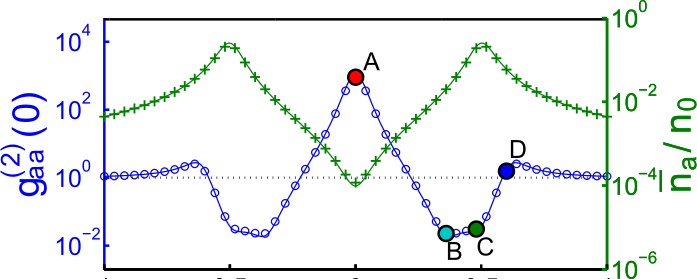
\includegraphics[width=0.45\textwidth]{./figs_Komar2013/fig2a.pdf}\quad
%   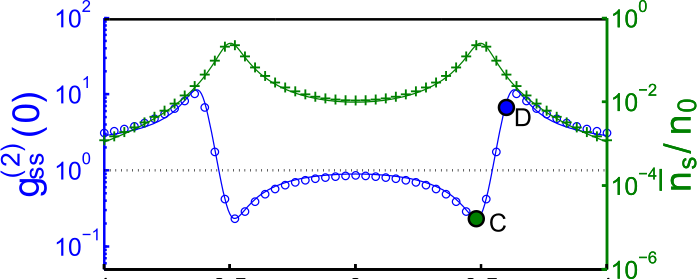
\includegraphics[width=0.45\textwidth]{./figs_Komar2013/fig2b.pdf}\\
%   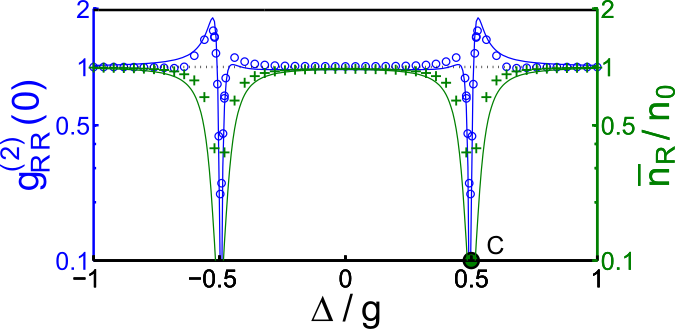
\includegraphics[width=0.45\textwidth]{./figs_Komar2013/fig2c.pdf}\quad
%   \includegraphics[width=0.45\textwidth]{./figs_Komar2013/fig2d.pdf}
%   \caption{
%   \label{fig:spectrum}(Color online)
%   (a) Normalized average photon number (green ``$+$")
%   and photon-photon correlation function (blue ``$\circ$")
%   for driven mode $c_a$
%   as a function of laser detuning at zero temperature.
%   Solid lines are calculated from analytic model
%   (see Eqs.~(\ref{eq:na}-\ref{eq:g2AA}))
%   and points show full numerical calculation.
%   The average photon number is
%   normalized by $n_0 = (\Omega/\kappa)^2$.
%   (b) Same as in (a) for the undriven mode $c_s$,
%   and
%   (c) for the reflected field $c_R$.
%   In all plots we took
%    $g/\kappa = 20$ and $\gamma/\kappa$ = 0.2.
%   Dots mark features seen at values of
%   detuning $\Delta/g = 0 \mathrm{ (A)}, \frac{1}{\sqrt{8}} \mathrm{ (B)},
%   \frac{1}{2} \mathrm{ (C)}$ and  $\frac{\sqrt{6}}{4} \mathrm{ (D)}$. 
%   The
%   small discrepancy between the analytic and numerical results
%   in (c) is due to the approximation
%   $g/\kappa \gg 1$   to  
%   simplify the expressions in Eqs.~(\ref{eq:na}-\ref{eq:g2AA}).
%   Bottom panels A-D illustrate the origin of these features as explained in the text.
%   Suppression  (enhancement) of the
%   steady state population of a specific level is
%   indicated by a red X (green circle).
%   }
% \end{figure}
% ==================================

\begin{figure}
\centering
  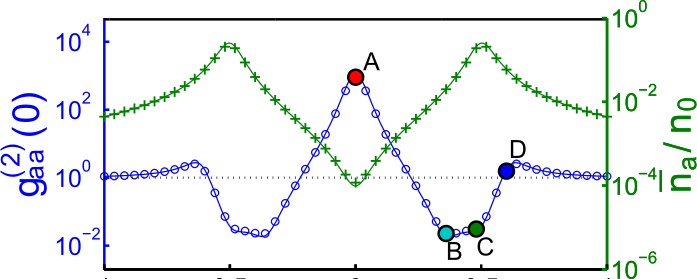
\includegraphics[width=0.8\textwidth]{./figs_Komar2013/fig2a.pdf}
  
  \caption
  [Photon statistics in anti-symmetric mode, $a$]
  {
  \label{fig:spectrum_a}
  Normalized average photon number (green ``$+$")
  and photon-photon correlation function (blue ``$\circ$")
  for driven mode $c_a$
  as a function of laser detuning at zero temperature.
  Solid lines are calculated from analytic model
  (see Eqs.~(\ref{eq:na}-\ref{eq:g2AA}))
  and points show full numerical calculation.
  The average photon number is
  normalized by $n_0 = (\Omega/\kappa)^2$. ($g/\kappa = 20$ and $\gamma/\kappa$
  = 0.2)
  }
\end{figure}

\begin{figure}
\centering
  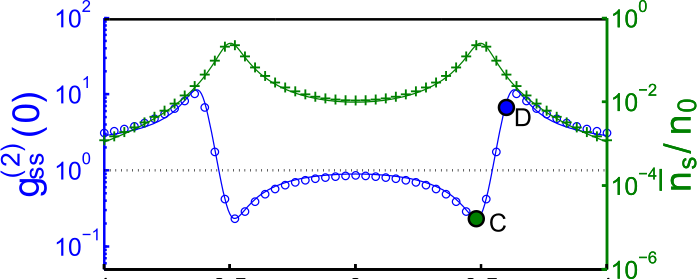
\includegraphics[width=0.8\textwidth]{./figs_Komar2013/fig2b.pdf}
  \caption
  [Photon statistics in symmetric mode, $s$]
  {
  \label{fig:spectrum_b}
  Normalized average photon number (green ``$+$")
  and photon-photon correlation function (blue ``$\circ$")
  for the undriven mode $c_s$
  as a function of laser detuning at zero temperature.
  Solid lines are calculated from analytic model
  (see Eqs.~(\ref{eq:na}-\ref{eq:g2AA}))
  and points show full numerical calculation.
  The average photon number is
  normalized by $n_0 = (\Omega/\kappa)^2$. ($g/\kappa = 20$ and $\gamma/\kappa$
  = 0.2)
  }
\end{figure}
 
\begin{figure}
\centering
  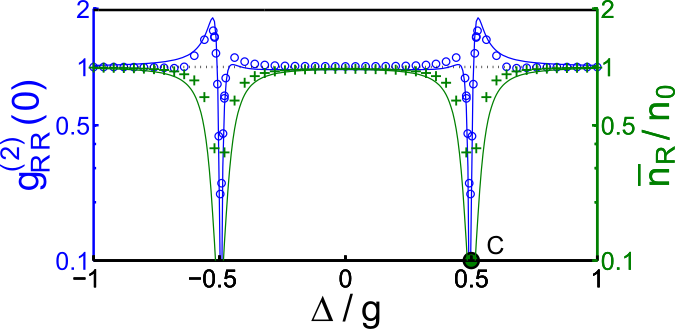
\includegraphics[width=0.8\textwidth]{./figs_Komar2013/fig2c.pdf}
  \caption
  [Photon statistics in reflected mode, $R$]
  {
  \label{fig:spectrum_c}
  Normalized average photon number (green ``$+$")
  and photon-photon correlation function (blue ``$\circ$")
  for the reflected field $c_R$,
  as a function of laser detuning at zero temperature.
  Solid lines are calculated from analytic model
  (see Eqs.~(\ref{eq:na}-\ref{eq:g2AA}))
  and points show full numerical calculation.
  The average photon number is
  normalized by $n_0 = (\Omega/\kappa)^2$.
  The
  small discrepancy between the analytic and numerical results is due to the
  approximation $g/\kappa \gg 1$   to  
  simplify the expressions in Eqs.~(\ref{eq:na}-\ref{eq:g2AA})
  ($g/\kappa = 20$ and $\gamma/\kappa$ = 0.2)
  }
\end{figure}
 


In addition to the transmission,
we plot the mean reflected photon number
in  \reffig{fig:spectrum_c}.
As discussed below, the reflected 
photon statistics
can also exhibit signatures of
nonlinearity.
We  calculate properties of the reflected light
using the
annihilation operator 
$c_R = c_a + i\frac{\Omega}{\kappa}$, obtained from standard input-output relations
for a symmetric two-sided cavity (see Appendix
\ref{App: Reflection}).
%$c_R = c_a + i\frac{\Omega}{\kappa}$.
The mean reflected photon number
$\bar n_R = \ev{c_R\+ c_R}$
is plotted in \reffig{fig:spectrum_c}.
%shows the reflected photon number, 
%$\bar n_R = \ev{c_R\+ c_R}$. 
At $\Delta/g = \pm \frac{1}{2}$, 
the average reflection has a minimum where the
average transmission has a maximum. 
Note that in contrast to a single cavity, 
even on resonance the transmission probability
is less than unity and the reflection probability
remains finite.



\subsection{Intensity correlations}
\label{sec:onetime_correlation}

To  characterize nonclassical 
photon statistics in the light transmitted through the OMS,
we study the equal-time photon-photon correlation
functions,
\bel
	\label{eq:g2(0)}
	g^{(2)}_{ii}(0)
	= \frac{\ev{c_i\+ c_i\+
	c_i  c_i }}{\ev{c_i\+ c_i}^2} ,
\eel
where all operators are evaluated at the same time and $i = a,s, R$. 
A normalized correlation of
$g^{(2)}_{ii}(0)< 1$ indicates photon anti-bunching, and the limit
$g^{(2)}_{ii}(0)\rightarrow 0$ corresponds to the 
complete photon blockade regime
in which two photons never occupy the cavity
at the same time.
The solid curves show $g^{(2)}_{aa}(0)$ in \reffig{fig:spectrum_a},
$g^{(2)}_{ss}(0)$ in \reffig{fig:spectrum_b} and $g^{(2)}_{RR}(0)$ 
\reffig{fig:spectrum_c} as a function of the laser  detuning and in the limit of
weak driving $\Omega/\kappa \ll1 $.
%for modes $c_a$, $c_s$ and the reflected
%mode $c_R$, respectively.
The most pronounced features of these correlation functions occur at 
$|\Delta|/g = 0, \frac{1}{\sqrt{8}}, \frac{1}{2} \mathrm{ and }\frac{\sqrt{6}}{4}$, 
as marked by
dots A, B, C and D, respectively. 
As we explain in detail in the following analysis, 
%Fig.~\ref{fig:spectrum}, 
we find that the photon bunching at A and
anti-bunching at B are the result of destructive 
quantum interference, while the 
features at points C and D arise from 
one- and two-photon resonances. 

%As illustrated in the bottom panel of
%Fig.~\ref{fig:spectrum}, 
%the photon bunching at A and
%anti-bunching at B arise from the suppression 
%of populations in states
%$|100\rangle$ and $|200\rangle$ respectively,
%due to destructive quantum interference
%(depicted by a red X).
%In contrast, the features at points C and D arise from 
%one- and two-photon
%resonances of the coupled system (indicated by a green O).
%These features can be understood
%in terms of a simple analytic model as we now discuss.

To gain insight into the two photon correlation functions shown in 
%We can capture the 
%features in  
\reffig{fig:spectrum_a}, \ref{fig:spectrum_b} and \ref{fig:spectrum_c},
we develop  an approximate analytic model 
for the system 
by considering only the
six levels shown in \reffig{fig:cartoon_b}.
Assuming that the system is initially prepared in $|000\rangle$, these are
the only levels significantly populated by weakly driving the
$c_a$ mode. We make the ansatz \cite{Carmichael1991}
\bel
\label{eq:psi}
\begin{split}
	\ket{\psi} =&\quad A_{000}\ket{000} + A_{100}\ket{100} + A_{011}\ket{011}\\
	&+ A_{200} \ket{200} + A_{111} \ket{111} + A_{022} \ket{022},
\end{split}
\eel
and describe the dynamics by evolving $|\psi\rangle$ under the action of the
non-Hermitian Hamiltonian, $\tilde{H} = H -i\left[\kappa c_a\+ c_a + \kappa
c_s\+ c_s + \frac{\gamma}{2} b\+ b\right]$. 
This approach allows us to evaluate
intensities up to order $\Omega^2$ and two-point correlation up to order
$\Omega^4$, since the neglected quantum jumps
lead to higher order corrections.
By neglecting the typically small mechanical decay rate
$\gamma \ll \kappa$,
the amplitudes in \refeq{eq:psi} then satisfy
\bal
	\label{eq:c000}\dot A_{000} &=& 0,\\[0.2cm]
	\dot A_{100} &=& -i\frac{g}{2} A_{011} -i\Omega A_{000} -
	\tilde\kappa A_{100},\\
	\label{eq:c011}
	\dot A_{011} &=& -i\frac{g}{2} A_{100} - \tilde\kappa A_{011},\\[0.2cm]
	\dot A_{200} &=& -i\frac{g}{\sqrt{2}} A_{111} -i\sqrt{2}\Omega A_{100}
	-2\tilde\kappa A_{200},\\
	\dot A_{111} &=& -i\frac{g}{\sqrt{2}} A_{200} -ig A_{022} - i\Omega A_{011} -
	2\tilde\kappa A_{111},\\
	\label{eq:c022}
	\dot A_{022} &=& -ig A_{111} -2\tilde\kappa A_{022},
\eal
where $\tilde \kappa = \kappa -i\Delta$. 
It is straightforward to solve
Eqs. (\ref{eq:c000}--\ref{eq:c022}) for the steady state amplitudes 
(see Appendix \ref{sect:App:steady_state}).
%\ref{sect:App:steady_state}
To lowest order in $\Omega/\kappa$  the mean
occupation numbers are $\bar n_a=|\bar A_{100}|^2$, $\bar n_s=|\bar A_{011}|^2$
and $\bar n_R=|\bar A_{100}+i\Omega/\kappa|^2$, where $\bar A$ denote
steady state amplitudes. We obtain
\bal
	\label{eq:na}
	\frac{\bar n_a}{n_0} &=&
		\frac{
			\kappa^2\left[R_\kappa(0)\right]^{1/2}
		}
		{
			R_\kappa\left(\frac{g}{2}\right)
		},\\
	\frac{\bar n_s}{n_0} &=&
		\frac{
			g^2\kappa^2
		}
		{
			4R_\kappa\left(\frac{g}{2}\right)
		},\\
	\frac{\bar n_R}{n_0} &\approx &
		\frac{
			\left[R_{\kappa/2}\left(\frac{g}{2}\right)\right]^2
		}
		{
			\left[R_\kappa\left(\frac{g}{2}\right)\right]^2
		},
\eal
where 
$R_K(\omega) = \left[K^2 +
(\Delta-\omega)^2\right]\left[K^2 + (\Delta+\omega)^2\right]$
and
$n_0 = (\Omega/\kappa)^2$.
%and $R_K(\omega) = \left[K^2 +
%(\Delta-\omega)^2\right]\left[K^2 + (\Delta+\omega)^2\right]$. 
From the 
factors $R_K(\omega)$ in the denominators  (numerators)
in these expressions, we obtain the positions
of the resonances  (antiresonances) in the 
average intracavity photon numbers, in excellent
agreement with the numerical results
shown in \reffig{fig:spectrum_a}, \ref{fig:spectrum_b} and
\ref{fig:spectrum_c}.
%We discuss these features in  detail below.
Our six-level model also provides the
equal-time correlations
(see Appendix \ref{sect:App:steady_state}),
%for
%which we find (see Appendix)
%\ref{sect:App:steady_state})
\bal
	g^{(2)}_{aa}(0) &=&
		\frac{
			R_\kappa\left(\frac{g}{\sqrt{8}}\right)
			R_\kappa\left(\frac{g}{2}\right)
		}
		{
			R_\kappa(0)
			R_\kappa\left(\frac{\sqrt{6}}{4}g\right)
		},
		\label{eq:g2aa}
		\\
	g^{(2)}_{ss}(0) &=&
		\frac{ 2
			R_\kappa\left(\frac{g}{2}\right)
		}
		{
			R_\kappa\left(\frac{\sqrt{6}}{4}g\right)
		},\\
	g^{(2)}_{RR}(0) &\approx &
		\frac{
			R_\kappa\left(\frac{g}{2}\right)
			R_{16\kappa^3/g^2}\left(\frac{g}{2}-\frac{2\kappa^2}{g}\right)
		}
		{
			\left[R_{\kappa/2}\left(\frac{g}{2}\right)\right]^2
		}.
		\label{eq:g2AA}
\eal
Again, these expressions are in agreement with
the features seen in the numerical results in \reffig{fig:spectrum_a},
\ref{fig:spectrum_b} and \ref{fig:spectrum_c}.
The positions of maxima and minima are
seen directly by the arguments of
the factors $R_K(\omega)$. 
Note that we assumed $g/\kappa \gg 1$ to
obtain the simplified
expressions in Eqs.~(\ref{eq:g2aa}-\ref{eq:g2AA}),
but we retained the 
shift of order $g (\kappa / g)^2$ in
the argument in \refeq{eq:g2AA}
%in the argument of the second $R$ symbol,
because this shift is larger than the width of 
the antiresonance.

%we approximated
%\refeq{eq:g2AA}, 


%To gain further insight on the positions of 
%the features seen in \reffig{fig:spectrum}
%and described by Eqs.~(\ref{eq:na}--\ref{eq:g2AA}), we 
%diagonalize $H$ in \refeq{eq:Hamiltonian_0} in the
%six-level subspace of \refeq{eq:psi}.
%This yields the following eigenstates (see
%\reffig{fig:cartoon}(b)):
%\bal
%	\label{eq:ket 0}\ket{0} &=& \ket{000},
%	\\
%	\label{eq:ket 1pm}\ket{1_\pm} &=& \frac{1}{\sqrt{2}}\left(\ket{100} \pm
%	\ket{011}\right),
%	\\
%	\label{eq:ket 2pm}\ket{2_\pm} &=& \frac{1}{\sqrt{6}}\left(\ket{200}\pm
%	\sqrt{3}\ket{111} + \sqrt{2}\ket{022}\right), 
%	\\
%	\label{eq:ket 2 0}\ket{2_0} &=& \frac{1}{\sqrt{3}}\left(\sqrt{2}\ket{200} -
%	\ket{022}\right).
%\eal
%In the diagonal basis, the weak drive couples all levels with total photon
%number $n$ to all levels with $n\pm 1$ photons.
%Some of the features arise simply from detuning
%the drive through one- or two-photon resonance
%with these eigenstates of the coupled OM system.

\begin{figure}
\centering
  \includegraphics[width=0.9\textwidth]{./figs_Komar2013/fig2d.pdf}
  \caption
  [Illustration of dominant processes]
  {
  \label{fig:spectrum_d}
  Illustration of the origin of the features marked with A,B,C and D on
  \reffig{fig:spectrum_a}, \ref{fig:spectrum_b} and \ref{fig:spectrum_c} as
  explained in the text.
  Suppression  (enhancement) of the
  steady state population of a specific level is
  indicated by a red X (green circle).
  }
\end{figure}
We now discuss each feature
in \reffig{fig:spectrum_a}, \ref{fig:spectrum_b} and \ref{fig:spectrum_c} in
terms of our six-level model together with the diagonal basis
in Eqs.~(\ref{eq:ket0}-\ref{eq:ket20}).
First, at 
detuning $\Delta = 0$ (point A in \reffig{fig:spectrum_a})
we see $g^{(2)}_{aa}(0)>1$, indicating bunching.  
This is due to destructive interference that
suppresses
the population in  $\ket{100}$ 
(panel A in \reffig{fig:spectrum_d}), and
can be understood as the system being
driven into a dark state,
$\ket{d} \propto g \ket{000} - \Omega \ket{011}$, similar to
electromagnetically induced 
transparency (EIT) \cite{Lukin2003, Weis2010}.
In the dark state, $\ket{011}$ remains populated,
% KS: I changed 110 -> 100 here
% SB: both incorrect, should be 011 
%by the weak drive, 
allowing transitions to $\ket{111}$
which in turn is strongly coupled to
$\ket{200}$.
The net result is a relative 
suppression of the probability to have one photon
compared to two photons
in the driven mode, 
leading to bunching at $\Delta = 0$.
Second, at detuning $\Delta = g/\sqrt{8}$ 
(point B), 
mode $c_a$ shows anti-bunching
due to a suppressed two-photon probability.
Again, this is due to destructive interference, or
the presence of a dark state in which
$\ket{200}$ remains unpopulated
(panel B).
Third, at detuning $\Delta = \frac{g}{2}$ 
(point C), 
all  modes show anti-bunching.
This is due to
a one-photon  resonant transition
$\ket{0} \rightarrow \ket{1_+}$ 
(panel C).
Finally, at detuning $\Delta = \frac{\sqrt{6}}{4}g$ 
(point D), 
both $c_a$ and $c_s$ show bunching due
to a two-photon resonant transition
$\ket{0} \rightarrow \ket{2_+}$
(panel D).
% KS: I replaced cartoon -> inset
% SB: inset -> panel



\subsection{Absence of two-photon resonance at $\Delta = 0$}

At first glance,
the level diagram in \reffig{fig:cartoon_b} together with
bunching 
in \reffig{fig:spectrum_a} 
suggest a two-photon resonance
at zero detuning $\Delta = 0$,
where the energy of the
eigenstate $\ket{2_0}$ is equal to the energy of two drive photons.
However, 
as discussed above,
the bunching at $\Delta = 0$ arises 
entirely from
the suppression of a one-photon population;
further, we 
find that the expected two-photon resonance is 
cancelled by  interference.
This can be seen from a second order perturbative 
calculation of the two-photon Rabi frequency $\Omega_{0,2_0}^{(2)}$ for the transition 
$|0\rangle\rightarrow |2_0\rangle$.  
The two-photon state $\ket{2_0}$ can be
populated by the drive 
$H_{\rm dr} = \Omega (c_a^\dag + c_a)$ 
from state $\ket{0}$ 
via two intermediate one-photon
eigenstates, $\ket{1_\pm}$ given by \refeq{eq:ket1pm},
with energies $\omega_{1_\pm} = -\Delta \pm \frac{g}{2}$
in the rotating frame.
The resulting Rabi frequency is
\bel
\label{eq:fgr}
	\Omega_{0,2_0}^{(2)} = \sum_{n=1_-, 1_+}
\frac{\ev{2_0| H_{\rm dr} |n}\ev{n| H_{\rm dr} |0}}{\omega_n},
\eel
which vanishes at $\Delta=0$ 
%the two-photon Rabi frequency vanishes
as a consequence of destructive interference between the two amplitudes. 
The exact cancellation is lifted
by including finite dissipation and the full spectrum;
%leading to finite population in $\ket{2_0}$;
nonetheless this simple argument shows that
the expected two-photon resonance at $\Delta = 0$
is strongly 
suppressed.


%$\kappa$ or $\gamma$ the exact cancellation is lifted, 
%and
%the resulting small, but finite population in $|2_0\rangle$ is responsible for
%the antibunching in point A.


%This can be seen from a second order 
%Fermi's golden rule calculation.
%The two-photon state $\ket{2_0}$ can be
%populated by the driving field from state $\ket{0}$ 
%via  two intermediate one-photon
%eigenstates, $\ket{1_+}$ and $\ket{1_-}$. 
%The total transition rate is
%$\Gamma_{\ket{0}\rightarrow \ket{2_0}} = 2\pi \left| M \right|^2
%\delta\left(\omega_0 - \omega_{2_0} \right)$,
%where in the rotating frame
%$\omega_0 = \omega_{2_0} = 0$, $\omega_{1_\pm} = -\Delta \pm \frac{g}{2}$,
%and 
%\bel
%\label{eq:fgr}
%	M = \sum_{n=1_-, 1_+}
%\frac{\ev{2_0| H_{\rm dr} |n}\ev{n| H_{\rm dr} |0}}{\omega_n} = 0.
%\eel
%We see that on resonance,
%$\Delta = 0$, the total rate vanishes
%%$\Gamma_{\ket{0}\rightarrow \ket{2_0}}=0$.
%%This is a consequence of 
%due to
%destructive interference of
%the two-photon
%amplitudes that would allow the transition.
%\sdb{Fix this.}
%Of course, for non-zero $\kappa$ or $\gamma$ this exact interference is lifted, and the resulting small, but finite population in $|2_0\rangle$ is responsible for the antibunching in point A.  



%This can be seen from a second order perturbative calculation of the two photon Rabi frequency $\Omega_{0,2_0}^{(2)}$ for the transition 
%$|0\rangle\rightarrow |2_0\rangle$.  The two-photon state $\ket{2_0}$ can be
%populated by the driving field from state $\ket{0}$ 
%via  two intermediate one-photon
%eigenstates, $\ket{1_+}$ and $\ket{1_-}$, which in the rotating frame
%have energies $\omega_{1_\pm} = -\Delta \pm \frac{g}{2}$, respectively. 
%Therefore, 
%\bel
%\label{eq:fgr}
%	\Omega_{0,2_0}^{(2)} = \sum_{n=1_-, 1_+}
%\frac{\ev{2_0| H_{\rm dr} |n}\ev{n| H_{\rm dr} |0}}{\omega_n},
%\eel
%and we see that on resonance $\Delta=0$ the two-photon Rabi-frequency vanishes as a consequence of destructive interference between the two amplitudes. Of course, for non-zero $\kappa$ or $\gamma$ this exact interference is lifted, and the resulting small, but finite population in $|2_0\rangle$ is responsible for the antibunching in point A.  



Further evidence of the absence of a
two-photon resonance at $\Delta=0$ is
the lack of bunching in the undriven mode in  
\reffig{fig:spectrum_b}.
If there were a two-photon resonance,
one would expect that bunching
should also occur in the undriven mode,
since the state $\ket{2_0}$ involves both $c_a$
and $c_s$ modes. 
This is indeed the case
at detuning $\Delta = \frac{\sqrt{6}}{4} g$
(see point D in \reffig{fig:spectrum_b}),
where
both modes show bunching as a result of
two-photon resonance.
In contrast, we see  no bunching in
the undriven mode at $\Delta = 0$. 
%due to the
%cancellation of two-photon resonance by interference.
This supports our conclusion that the observed
bunching at $\Delta=0$ arises 
from suppression of 
population in $\ket{100}$ due to interference,
as discussed in Section \ref{sec:onetime_correlation},
and not from two-photon resonance.
%Instead, this bunching arises
%from a suppression of the one-photon amplitude
%$A_{100}$
%as discussed in Section \ref{sec:onetime_correlation}.
As discussed above, this interference
does not suppress population in 
$\ket{011}$,
so we do not expect
bunching in the $c_s$ mode from this effect.
% ==================================
\begin{figure} 
\centering
  \includegraphics[width=0.8\textwidth]{./figs_Komar2013/fig3.pdf}
  \caption
  [Aggregate photon statistics]
  {
  \label{fig:populations}
  Average number (green dashed) and intensity correlation
  (blue solid)
  of total photon number in the coupled OM system.
  Parameters are the same as in \reffig{fig:spectrum_a},
  and dots mark the same detunings.
  One- and two-photon resonances are
  seen at C and D,
  but we see no bunching in the
  total photon number at 
  $\Delta = 0$ (point A).
%  is where a two-photon transition
%  $\ket{0}\rightarrow\ket{2_0}$ is naively expected.
  This reflects the lack
  of two-photon resonance due to 
  destructive interference (see \refeq{eq:fgr}).  } 
\end{figure}
% ==================================

Finally, to confirm our intuitive picture we plot the
intensity correlation function, 
$g^{(2)}_{\mathrm{tot}}(0) =
\ev{n_{\mathrm{tot}}(n_{\mathrm{tot}}-1)}/\ev{n_{\mathrm{tot}}}^2$,
of the total photon number, $n_{\mathrm{tot}} = n_a +
n_s$,
in the coupled OM system in
\reffig{fig:populations}. 
The probability to find one photon in the combined
cavity is maximal at $\Delta/g=\pm \frac{1}{2}$ 
due to one-photon resonance.
Similarly, we  
observe antibunching at point C
and bunching at point D,
due  to interference and two-photon resonance
respectively,
as discussed 
in Section \ref{sec:onetime_correlation}.
%The two-photon probability also has a peak at $\Delta/g=\pm \frac{1}{2}$, since
%a second photon can enter the cavity off-resonantly.
%In addition, the two-photon probability has peaks at 
%$\Delta / g  = \pm \sqrt{6} /4$ due to two-photon resonances.  
However, we find neither bunching nor antibunching
at $\Delta = 0$, 
demonstrating the absence of a two-photon resonance
despite the fact that $\ket{2_0}$ lies at twice the
drive frequency.



%Finally, to confirm our intuitive picture we plot the
%total photon number and $g^{(2)}(0)$ in steady state in
%\reffig{fig:populations}.
%The number of photons ($n_\mathrm{tot} = n_a + n_s$) in the combined
%cavity is maximal and $g^{(2)}_\mathrm{tot}(0) =
%\ev{n_\mathrm{tot}(n_\mathrm{tot}-1)}/\ev{n_\mathrm{tot}}^2$
%is minimal at $\Delta/g=\pm \frac{1}{2}$ due to one-photon resonance causing anti-bunching.
%The $g^{(2)}_\mathrm{tot}(0)$ has peaks at 
%$\Delta / g  = \pm \sqrt{6} /4$ due to two-photon resonances.  
%However, there
%is no peak ($g^{(2)}_\mathrm{tot}(0) \approx 1$) at $\Delta = 0$, 
%demonstrating the absence of a two-photon resonance
%despite the fact that $\ket{2_0}$ lies at the twice the
%drive frequency.

 


\subsection{Finite temperature}

\begin{figure}
\centering
  \includegraphics[width=0.8\textwidth]{./figs_Komar2013/fig4a.pdf}
  \caption
  [Temperature dependence of the relevant levels]
  {
  \label{fig:thermal_g2_a}
  Level diagram showing the
  six states populated by the drive from level $|0,0,n\rangle$ (left), 
  and the associated
  eigenmodes (right) with $n$-dependent splittings.
}
\end{figure} 

\begin{figure}
\centering
  \includegraphics[width=0.8\textwidth]{./figs_Komar2013/fig4b.pdf}
  \caption
  [Effect of non-zero temperature on photon statistics of mode $a$]
  {
  \label{fig:thermal_g2_b}
  Driven mode correlation function $g^{(2)}_{aa}(0)$
  for thermal mechanical occupation $N_{\rm th} = 0,1,2$.
  Solid lines show the analytic calculation with $\gamma \rightarrow 0$,
   and  dots show the full numerical results for $N_{\rm th} = 2$ only.
  The inset shows the minimal $g^{(2)}_{aa}(0)$ as a function of $N_{\rm th}$ 
  for several
  coupling strengths. 
  Parameters are $g/\kappa=20$, and (for numerics) $\gamma/\kappa =  10^{-3}$.
}
\end{figure} 

\begin{figure}
\centering
  \includegraphics[width=0.8\textwidth]{./figs_Komar2013/fig4c.pdf}
  \caption
  [Effect of non-zero temperature on photon statistics of mode $s$]
  {
  \label{fig:thermal_g2_c}
  Undriven mode correlation function $g^{(2)}_{ss}(0)$
  for thermal mechanical occupation $N_{\rm th} = 0,1,2$.
  Solid lines show the analytic calculation with $\gamma \rightarrow 0$,
   and  dots show the full numerical results for $N_{\rm th} = 2$ only.
  The inset shows the minimal $g^{(2)}_{ss}(0)$ as a function of $N_{\rm th}$ 
  for several
  coupling strengths. 
  Parameters are $g/\kappa=20$, and (for numerics) $\gamma/\kappa =  10^{-3}$.
}
\end{figure} 


So far in our analysis
we have focused on the case where the mechanical
system is prepared in its vibrational 
ground state, $|0_m\rangle$. 
This
condition can be achieved using high frequency resonators 
operated at cryogenic
temperatures \cite{O'Connell2010}, 
and in the limit of weak driving $\Omega/\kappa\ll1$ such
that optical
heating of the mechanical mode can be neglected. 
The mechanical ground state  could also be 
prepared using OM cooling \cite{Metzger2004, Gigan2006, 
Arcizet2006, Kleckner2006, Corbitt2007, 
Schliesser2008,Thompson2008,Wilson2009,
O'Connell2010,Teufel2011,Chan2011},
using an optical mode far-detuned
from the ones we consider  here for 
nonlinear interactions
\cite{Stannigel2012}.
Nonetheless,
in the
following we extend our analytic treatment to the case of finite temperature, 
and show that many of the
nonclassical features are robust even
in the presence of small
but finite thermal occupation of the mechanical mode.


To generalize our previous results we now consider
a finite equilibrium occupation number $N_{\rm th} >0$ of 
the mechanical mode,
but still assume that $\gamma(N_{\rm th}+1) \ll\kappa,g$. 
Within this approximation we proceed
as above, and
make a similar six-level ansatz as in Eq.~\eqref{eq:psi}
for each phonon number $n$,
%\bel
%\label{eq:psi_thermal}
%\begin{split}
%	&\ket{\psi_n} =\\
%	&\quad A_{0,0,n}\ket{0,0,n} + A_{1,0,n}\ket{1,0,n} +
%	A_{0,1,n+1}\ket{0,1,n+1}\\
%	&+ A_{2,0,n} \ket{2,0,n} + A_{1,1,n+1} \ket{1,1,n+1} \\
%	&+ A_{0,2,n+2}\ket{0,2,n+2},
%\end{split}
%\eel
\bel
\label{eq:psi_thermal}
\begin{split}
	\ket{\psi_n} &=
	 A_{0,0,n}\ket{0,0,n} + A_{1,0,n}\ket{1,0,n} \\
	&+ A_{0,1,n+1}\ket{0,1,n+1} + A_{2,0,n} \ket{2,0,n} \\
	&+ A_{1,1,n+1} \ket{1,1,n+1} 
	+ A_{0,2,n+2}\ket{0,2,n+2},
\end{split}
\eel
 where $\ket{\psi_n}$ includes states up
 to two photons that are connected 
 by the weak drive and coupling $g$,
 starting from the state $|0 0 n\rangle$. 
 As
 shown in Fig.~\ref{fig:thermal_g2_a} the coupling between the states
 within each six-level subspace
 depends explicitly on the phonon number $n$. 
Following the same approach as above,
the amplitudes in Eq.~\eqref{eq:psi_thermal} evolve according to
\bal
       \dot A_{0,0,n} &=& 0,\\
\dot A_{1,0,n} &=& -i \frac{g}{2} \sqrt{n+1} A_{0,1, n+1} -i\Omega A_{,00,n}
-\tilde\kappa A_{1,0,n},\\
\dot A_{0,1,n+1} &=& -i\frac{g}{2} \sqrt{n+1} A_{1,0,n} - \tilde\kappa
A_{0,1,n+1},\\
\dot A_{2,0,0} &=& -i g\sqrt{\frac{n+1}{2}} A_{1,1,n+1} -i\sqrt{2}\Omega
A_{1,0,n}
-2 \tilde\kappa A_{2,0,n},\\
\dot A_{1,1,n+1} &=& -ig\sqrt{\frac{n+1}{2}}  A_{2,0,n} -i
g\sqrt{\frac{n+2}{2}}A_{0,2,n+2} - i\Omega A_{0,1,n+1} - 2\tilde\kappa
A_{1,1,n+1},\qquad \\
\dot A_{0,2,n+2} &=& -ig\sqrt{\frac{n+2}{2}} A_{1,1,n+1} -2\tilde\kappa
A_{0,2,n+2}.
\eal
We solve for the steady state amplitudes within each 
subspace  $n$ and average
the result over the initial thermal phonon distribution,
assuming no coupling between subspaces due to
the small phonon relaxation rate.
We obtain the
average photon numbers
\begin{align}
	\bar n_a=\sum_n \zeta_n |\bar A_{1,0,n}|^2,
	\qquad
	\bar n_s=\sum_n \zeta_n |\bar A_{0,1,n+1}|^2,
\end{align}
where $\zeta_n=e^{-\beta \hbar\omega_m n}(1-e^{-\beta \hbar\omega_m })$ and
$\beta^{-1}=k_B T$.
Similarly, the $g^{(2)}_{ii}(0)$ functions are given by 
\begin{align}
	g^{(2)}_{aa}(0)=&2\sum_n\zeta_n |\bar A_{2,0,n}|^2 / \bar n_a^2,\\
	g^{(2)}_{ss}(0)=&2\sum_n\zeta_n |\bar A_{0,2,n+2}|^2 / \bar n_s^2.
\end{align} 
We provide the expressions for the steady state amplitudes
$\bar A_{2,0,n}$ and $\bar A_{0,2,n+2}$ in the
 Appendix \ref{sect:App:steady_state}.

 





We plot the correlation functions,
$g^{(2)}_{aa}(0)$ in \reffig{fig:thermal_g2_b} and $g^{(2)}_{ss}(0)$ in
\reffig{fig:thermal_g2_c} for different thermal phonon numbers, $N_{\rm th}$. 
Solid lines were calculated from the above
analytic approach with $\gamma \rightarrow 0$, 
and we find excellent agreement with
the full numerical results including small but finite
$\gamma$ (dots, shown only for
thermal occupation $N_{\rm th} = 2$).
We see that the zero temperature
features such as antibunching
survive at finite temperature for sufficiently strong coupling~\cite{Stannigel2012}.
In the insets we plot the minimum antibunching
as a function of thermal occupation number for
several ratios $g / \kappa$. 
Antibunching remains visible up
to a critical thermal phonon number, 
set by $g/\kappa$, 
beyond which the contributions from 
different phonon numbers smear out the effect
and antibunching vanishes.
%\pk{This antibunching vanishes for $N_\mathrm{th}
%\sim g^2/\kappa^2$, which we can understand from estimating $\bar{n}_a
%\sim\frac{\Omega^2}{g^2}\left(\frac{g^2}{\kappa^2N_\mathrm{th}}+1\right)$, and the
%two photon probability $\sim\frac{\Omega^2}{g^2}\bar{n}_a$ at $\Delta = g/2$,
%for $g\gg \kappa$.} 
In addition, for detunings $|\Delta|>g/2$, a series of new
resonances appear in the correlation functions, 
and for small but finite occupation numbers we  find
new antibunching features that are absent for $N_{\rm th}=0$.
These new features  can be understood from the $n$-dependent splitting of the
one- and two-photon manifolds as indicated in \reffig{fig:thermal_g2_a}.
For higher temperatures the individual resonances start to overlap, and we
observe an overall increase over a broad region of large positive and negative
detunings due to the cumulative effect of different phonon numbers.
% % ==================================
% \begin{figure}
% \centering
%   \includegraphics[width=0.7\textwidth]{./figs_Komar2013/fig4a.pdf}\\
%   \includegraphics[width=0.7\textwidth]{./figs_Komar2013/fig4b.pdf}\\
%   \includegraphics[width=0.7\textwidth]{./figs_Komar2013/fig4c.pdf}
%   \caption{
%   \label{fig:thermal_g2}(Color online)
%   Correlation functions for finite temperature. (a) Level diagram showing the
%   six states populated by the drive from level $|0,0,n\rangle$ (left), 
%   and the associated
%   eigenmodes (right) with $n$-dependent splittings.
%   (b) Driven mode correlation function $g^{(2)}_{aa}(0)$
%   for thermal mechanical occupation $N_{\rm th} = 0,1,2$.
%   Solid lines show the analytic calculation with $\gamma \rightarrow 0$,
%    and  dots show the full numerical results for $N_{\rm th} = 2$ only.
%   The inset shows the minimal $g^{(2)}_{aa}(0)$ as a function of $N_{\rm th}$ 
%   for several
%   coupling strengths. 
%   (c) Same as (b) for the undriven mode correlation function $g^{(2)}_{ss}(0)$. 
%   Parameters are $g/\kappa=20$, and (for numerics) $\gamma/\kappa =  10^{-3}$.
% }
% \end{figure} 
% % ================================== 



%%%%%%%%%%%%%%%%%%%%%%%%%%%%%%%%%%%%%%%%
%%%%%%%%%%%%%%%%%%%%%%%%%%%%%%%%%%%%%%%%
\section{Delayed coincidence and single phonon states}
\label{sect:Delayed_coincidence}


In addition to the equal-time correlations discussed above,
quantum signatures can also be manifested in photon
intensity correlations with a finite time delay.
We now turn to a discussion of  delayed coincidence
characterized by the 
two-time
intensity correlations functions,
\bel
\label{eq:g2_tau}
	g^{(2)}_{ii}(\tau) = \frac{\ev{c_i\+(0) c_i\+ (\tau) c _i(\tau)
	c_i(0)}}{\ev{c_i\+ c_i}^2},
\eel
for both driven and undriven modes, $i = a,s$.
Expressing this correlation in terms of a classical
light intensity $I$,
$g^{(2)}(\tau) = \ev{ I(\tau) I(0) } / \ev{ I }^2$,
and
using the Schwarz inequality, we
obtain the inequalities \cite{Carmichael1991, Brecha1999},
\begin{align}
  \label{eq:classical_criterium}
 	g^{(2)}(\tau) &\leq g^{(2)}(0),	%\quad &(\mathrm{classical}),
	\\
	 |g^{(2)}(\tau)-1| & \leq |g^{(2)}(0)-1| .%\quad &(\mathrm{classical}),
\end{align}
Similar to the classical inequality
$g^{(2)}(0) > 1$ at zero delay, 
violation of either of these inequalities
at finite delay is
a signature of quantum light. 
We calculate the delayed coincidence correlation
functions
for both the driven and undriven modes.


\subsection{Driven mode}
The
correlation function $g^{(2)}_{aa}(\tau)$ is shown in \reffig{fig:g2aatau}(a)
for two values of the detuning $\Delta$.
The most striking feature
is the apparent vanishing of  $g^{(2)}_{aa}(\tau)$
at several values of $\tau$ when the
detuning is $\Delta = 0$ (curve A in \reffig{fig:g2aatau}(a)).
These are due to Rabi oscillations at frequency
$g/2$ following the detection of a photon.
This vanishing of the finite delay correlation function
is reminiscent of  wavefunction collapse that
occurs in a cavity containing an 
atomic ensemble \cite{Carmichael1991},
and while its origins are similar, there are important
differences as we now discuss.




We can understand the finite delay intensity
correlations
in terms of the simple six-level model discussed
in the previous section.
We extend
this model to describe finite delay correlations
by considering the effect of photodetection on
the steady state of the system.
Detection of a photon in the driven mode projects
the system onto the conditional state \cite{QuantumNoise},
\bel
	\label{eq:psi^a}
	\ket{\psi^a} = \frac{c_a \ket{\psi}}{||c_a \ket{\psi} ||},
\eel
where $\ket{\psi}$ is given by \refeq{eq:psi} with steady state amplitudes
and $|| \cdot ||$ denotes normalization after the jump.
The conditional state $\ket{\psi^a}$ has an {\it increased}
amplitude $A_{100}$ after the jump
(see jump at $\tau = 0$ in \reffig{fig:g2aatau} (b)).
Following this initial photodetection, the amplitude 
$A_{100}$
subsequently undergoes Rabi oscillations with frequency $g/2$,
and decays back to its steady state at rate $2\kappa$. 
For sufficiently large bunching at zero delay and
strong coupling $g > \kappa$, the  Rabi oscillations of the amplitude
$A_{100}(\tau)$ can cause it to cross zero 
several times before it decays back
to steady state.
As the probability to detect a second photon is dominated by $A_{100}$,
its zeros are responsible for the zeros in the correlation
function $g^{(2)}_{aa}(\tau)$ zero at these delay times.





The zeros in $g^{(2)}(\tau)$ appear similar
to those exhibited  in
a cavity strongly coupled to
an atomic ensemble \cite{Carmichael1991, Rice1988, Brecha1999} or a single atom
\cite{Chang2007}. 
However, in stark contrast to the atomic case,
the zeros in \reffig{fig:g2aatau}(a)
are the result of Rabi oscillations  following
the initial quantum jump.
This is qualitatively different from
the atomic case, where the change in
sign of the relevant amplitude (the analogy of $A_{100}$)
occurs {\it immediately} after the jump itself, and the amplitude
is damped back to steady state at the atomic
decay rate $\Gamma$, without Rabi oscillation. 
As a consequence, the vanishing correlation
function in the atomic case occurs
at a delay set by $\tau_0 \sim \gamma^{-1}\ln C$, 
requiring only strong cooperativity $C = g^2/ \kappa \gamma > 1$
to be visible.
On the other hand,
the zeros in \reffig{fig:g2aatau}(a)
occur at delay times set by  $\tau \sim 1/g$,
requiring strictly strong coupling $g > \kappa$.








Before moving on to correlations of the undriven mode,
we briefly discuss the correlations of the driven mode at the
 other value of  detuning shown in 
\reffig{fig:g2aatau}(a).
 At detuning
$\Delta = \frac{g}{\sqrt{2}}$ (curve E),
which shows bunching at zero time,
$g^{(2)}_{aa}(0) \gtrsim 1$, 
increases  above its initial value at
finite delay.
This is a violation of the classical inequality in
\refeq{eq:classical_criterium}, 
and is an example of ``delayed bunching,"
or an increased probability to detect a second
photon at a finite delay time.
A similar effect was recently studied
in a single mode OMS \cite{Kronwald2012}.
However, like the Rabi oscillations,
the increased correlation function decays back to its steady state
value of 1 on
the timescale of $\kappa^{-1}$.
%%%%%%%%%%%%%%%%%%%%%%%%%%%%%
%%%%%%%%%%%%%%%%%%%%%%%%%%%%%
\begin{figure} 
\centering
  \includegraphics[width=0.9\textwidth]{./figs_Komar2013/fig5a.pdf}\\[-0.5cm]
  \includegraphics[width=0.9\textwidth]{./figs_Komar2013/fig5b.pdf}
  \caption
  [Autocorrelation of mode $a$]
  {
  \label{fig:g2aatau}
  (a) Finite time delay intensity
  correlation function $g^{(2)}_{aa}(\tau)$  for detunings
  $\Delta/g = 0 \mathrm{ (A)}$ and $\frac{1}{\sqrt{2}}
  \mathrm{ (E)}$.
  Detuning for curve A is the same as marked in \reffig{fig:spectrum_a},
  while E shows a new effect not seen at equal times.
  Thin dashed line indicates the classical bound 
  (see \refeq{eq:classical_criterium}) for curve E. 
  (b) Evolution of amplitude $A_{100}$ (normalized by its
  steady state value)
  at detuning A, $\Delta/g = 0$,
  after detecting a driven $c_a$ photon at $\tau = 0$. 
  Vertical dash-dotted lines mark delay times ($\tau_1, \tau_2$) where this amplitude
  vanishes resulting in the vanishing of $g^{(2)}_{aa}(\tau)$
  in (a).
  Parameters are $g/\kappa = 8$ and $\gamma/\kappa$ = 0.02. 
  } 
\end{figure}
%%%%%%%%%%%%%%%%%%%%%%%%%%%%%
%%%%%%%%%%%%%%%%%%%%%%%%%%%%%




\subsection{Heralded single phonon states}

We now turn to a discussion of the delayed coincidence
correlations of the undriven mode $c_s$.
We note that correlations of the driven
and undriven modes can be measured separately
provided sufficient frequency resolution, smaller than
  the mechanical frequency.
The correlation function
$g^{(2)}_{ss}(\tau)$
of the undriven mode
is shown in \reffig{fig:g2sstau} for several
values of detuning.
Similar to the driven mode, the
correlation function of the undriven mode
exhibits Rabi oscillations 
that decay on the short optical
timescale
$1/\kappa$.
For detuning $\Delta = 0$ and 
$\Delta/g = \frac{\sqrt{6}}{4}$
(curves A and D in \reffig{fig:g2sstau}),
the correlation $g^{(2)}_{ss}(\tau)$
is described by
our previous six-level 
model of Eqs. (\ref{eq:c000}--\ref{eq:c022}).
However,  at detuning $\Delta = \frac{g}{\sqrt{2}}$
(curve E), we see that
$g^{(2)}_{ss}(\tau)$ has a long
tail that decays
on the much longer mechanical timescale $1/\gamma$.
This is due to the heralded preparation
of a single phonon by detection of a photon in the
undriven mode, as we now discuss.
%and can be understood
%by a simple extension of the six-level model
%discussed above.
%%%%%%%%%%%%%%%%%%%%%%%%%%%%%
%%%%%%%%%%%%%%%%%%%%%%%%%%%%% 
\begin{figure}[htb] \centering
  \includegraphics[width=0.8\textwidth]{./figs_Komar2013/fig6.pdf}
  \caption[Autocorrelation of mode $s$]
  { 
  \label{fig:g2sstau}
  Finite time delay intensity correlation function $g^{(2)}_{ss}(\tau)$
  for detunings $\Delta/g = 0 \mathrm{ (A)}, \sqrt{6}/4 \mathrm{ (D)}$
  and
  $\frac{1}{\sqrt{2}} \mathrm{ (E)}$.
  Thin dashed lines indicate the classical bounds
  (see  \refeq{eq:classical_criterium}).
  Labels A, D, E correspond to the same detunings
  marked in 
  \reffig{fig:spectrum_a}
  and
  \reffig{fig:g2aatau}.
  Parameters are $g/\kappa = 8$, and $\gamma/\kappa$ = 0.02.
  }
\end{figure}
%%%%%%%%%%%%%%%%%%%%%%%%%%%%%
%%%%%%%%%%%%%%%%%%%%%%%%%%%%%



The increase in delayed coincidence can be understood
by extending the above analytic six-level model to account
for the conditional state of the system after detection
of a photon in the undriven mode.
To do this,
we simply add three additional states to
the six-level ansatz in  \refeq{eq:psi},
\bel
\label{eq:psi9}
	\ket{\psi} = \dots + A_{001}\ket{001} + A_{101}\ket{101} + A_{012}\ket{012},
\eel
since these are the states populated by detection
of a $c_s$ photon from the original six states (see \reffig{fig:levels_jumps}).
Using the same 
%non-Hermitian dynamics
approach as before, we obtain the following equations for the
amplitudes,
\bal
	\label{eq:c001}
	\dot A_{001} &\approx& -\frac{\gamma}{2}A_{001},\\[0.2cm]
	\dot A_{101} &=& -i\frac{g}{\sqrt{2}} A_{012} -i\Omega A_{001} -
	\tilde\kappa A_{101},\\
	\label{eq:c012}
	\dot A_{012} &=& -i\frac{g}{\sqrt{2}} A_{101} - \tilde\kappa A_{012},
\eal
where we used $\gamma \ll \kappa$ and
kept the leading term in \refeq{eq:c001}.
We obtain $g^{(2)}_{ss}(\tau)$
by solving these equations for initial
conditions determined by the conditional state $\ket{\psi^s}$
after a quantum jump, 
\bel
	\label{eq:psi^s}
	\ket{\psi^s} = \frac{c_s \ket{\psi}}{||c_s \ket{\psi}||},
\eel
which is a superposition of states $\ket{001}, \ket{101}, \ket{012}$
(see Appendix \ref{sect:App:steady_state} 
%\ref{sect:two-time_analytic} 
for details), but in the limit of weak driving consist mainly of $|001\rangle$. 


Detection of a photon in the undriven mode
implies that the three-wave mixing interaction
converted a photon from the driven mode into
the undriven mode by simultaneously adding a phonon.
The relevant three-level subspace after the jump 
(see \reffig{fig:levels_jumps}) has a similar structure as in the steady state, 
but the presence of an extra phonon
modifies the splitting of the one-photon 
states $|1^\prime_{\pm}\rangle=(|101\rangle \pm |012\rangle)/\sqrt{2}$  to
$\frac{g}{\sqrt{2}}$ 
(instead of $g/2$ without a phonon).
%
%The increase in delayed coincidence
%at specific laser detuning is a direct consequence
%of this conversion,
%as illustrated in \reffig{fig:levels_jumps}.
%In steady state, the system occupies the
%six levels of \refeq{eq:psi}, shown 
%on the left in \reffig{fig:levels_jumps}.
%After detection of an undriven $c_s$ photon,
%the 
%emitted  phonon slowly decays back
%to its ground state at rate $\gamma$, 
%during which time the system is in the conditional
%subspace shown on the
%right in \reffig{fig:levels_jumps}.
%%%%%%%%%%%%%%%%%%%%%%%%%%%%%
%%%%%%%%%%%%%%%%%%%%%%%%%%%%% 
\begin{figure}[htb]
\centering  
  \includegraphics[width=0.85\textwidth]{./figs_Komar2013/fig7.pdf}\\
  \caption[Diagram of the metastable subspace]
  {
  \label{fig:levels_jumps}
  Effect of detection of a $c_s$ photon
  at detuning E ($\Delta/g = \frac{1}{\sqrt{2}}$).
  In steady state (gray region on left), 
  the drive is far off-resonant.
  However, after detection of a $c_s$ photon the system
  jumps into the conditional subspace (pink region on right).
  Due to the presence of an extra phonon in this subspace,
  the drive is resonant and the probability to detect a second
  photon is much higher than in steady state.
  This increased probability persists
  as long as the extra phonon,
  which decays slowly at rate $\gamma$.
  }
\end{figure}
%%%%%%%%%%%%%%%%%%%%%%%%%%%%%
%%%%%%%%%%%%%%%%%%%%%%%%%%%%%
This changes
the one-photon resonance condition
for the drive to $\Delta = \frac{g}{\sqrt{2}}$.
Therefore, at this value of the detuning,
the process of
exciting the system and emitting a single $c_s$ photon
is off-resonant;
while after the detection of a first $c_s$ photon
the system is prepared in $|001\rangle$, bringing
it into resonance with the drive.
%brings the system into resonance with the drive,
This {\it enhances}
the probability for subsequent excitation and emission
of a second $c_s$ photon, increasing
the correlation function at finite delay.
%successive excitation of the second photon 
%occurs exactly on resonance. 
%while 
%resonant in the presence of an extra phonon,
%such that 
%the probability to detect a second 
%photon 
%This process {\it enhances} the probability 
%of photon coincidences in the undriven mode, 
The maximum delayed coincidence
occurs after a delay of $\tau \sim 1/\kappa$,
when the photons have reached the
metastable steady state
in the conditional  subspace with one 
extra phonon.
Eventually, the delayed coincidence
returns to its true steady state value
of one
%of $g^{(2)}_{ss}(\tau) \rightarrow 1$
on the timescale
$\tau \sim 1/\gamma$, which is the mechanical decay time of the
state $|001\rangle$. 
%\pk{Detuning $\Delta/g = 1/\sqrt{2}$ is chosen in order
%to optimize the visibility of the long tail of $g^{(2)}_{ss}$. 
The long tails
observed for other values of detuning (curves A and D) are
also
due to the presence of an extra phonon,
but in these cases the system remains off-resonant
after the initial $c_s$ photon and the effect is less
 pronounced.
Note that the
probability  to detect a photon from the {\it driven} mode also increases in 
the conditional state, so a similar effect is seen in the delayed 
cross-correlation function $g^{(2)}_{as}(\tau)$, where the photon in the 
undriven mode is detected first.

%Detection of a photon in the undriven mode
%implies that the three-wave mixing interaction
%converted a photon in the driven mode into
%one in the undriven mode by generating a phonon.
%After this first detection, the 
%emitted single phonon slowly decays back
%to its ground state at rate $\gamma$.
%During this slow decay, the presence
%of the extra phonon modifies the resonance
%condition of the coupled OM system, 
%changing the probability to detect a second photon.
%Specifically, if the drive detuning is chosen so that the
%system is off-resonant in steady state
%(at zero temperature), but
%resonant in the presence of an extra phonon,
%then 
%the probability to detect a second 
%photon {\it increases}
%after detection of a photon in the undriven mode.
%This increase in the  coincidence correlation
%at finite delay seen in 
%$g^{(2)}_{ss}(\tau)$
%violates the classical inequality in
%\refeq{eq:classical_criterium}.



%%%%%%%%%%%%%%%%%%%%%%%%%%%%%%%%%%%%%%%%
%%%%%%%%%%%%%%%%%%%%%%%%%%%%%%%%%%%%%%%%
\section{Reaching strong coupling}
\label{sect:Experimental values}


The nonclassical correlations predicted in this chapter 
require  strong optomechanical coupling, $g > \kappa$, 
as well as sideband resolution, $\omega_m \gg \kappa,\gamma$. 
While the combination of these conditions has not 
yet been demonstrated, 
several experimental efforts 
%in OMSs 
are currently 
directed at reaching this regime. 
By using micro- and nano-fabricated OMSs such 
as microtoroids or photonic crystal beams, 
high frequency mechanical systems  with 
$\omega_m\approx 50$ MHz - 5 GHz can be combined 
with low loss optical modes, such that the 
condition $\omega_m \gg \kappa \gg \gamma$ is satisfied
\cite{Safavi-Naeini2011a, Schliesser2008, Eichenfield2009}.
At the same time the mechanical system can already 
be prepared close to the quantum ground state by working at cryogenic temperatures. 
In micro-fabricated OMSs, single-photon couplings of 
about $g/\kappa \approx 0.001$ have been demonstrated 
\cite{Eichenfield2009, Ding2011,Verhagen2011}
%\cite{Teufel2011,Teufel2011a}.
The largest value to date of $g/\kappa \approx 0.007$ 
has been reached in photonic crystal beam
resonators \cite{Chan2012}, where
colocalized optical and vibrational resonances are
highly confined to maximize coupling
while the surrounding structure is engineered  
to minimize loss.
Conversely, in cold atomic experiments
the effective strong OM coupling regime has been
reached \cite{Purdy2010}, while sideband resolution remains
a challenge \cite{Stamper-kurn}. 


%In experiments with a 
%micromechanical membrane capacitively coupled to
%a superconducting resonant microwave circuit,
%a ratio of $g/\kappa \approx 0.001$
%has been achieved \cite{Teufel2011,Teufel2011a}.
%The strongest
%ratio to date of ($g/\kappa \approx 0.005$) were 
%reached in photonic crystal beam
%resonators \cite{Chan2012}, where
%colocalized optical and vibrational resonances are
%highly confined to maximize coupling
%while the surrounding structure is engineered
%to minimize loss.
%However in systems with the highest achieved
%ratio of $g/\kappa$, two orders of magnitude
%improvement is required to reach
%the strong coupling
%regime. 


There are several existing
proposals for how to meet the challenge
of $g/\kappa > 1$ 
in the photonic crystal beam setup.
First, 
the single-photon optomechanical coupling can 
be increased by making use of
nanoslots in the structure \cite{Robinson2005, Davanc2012} 
to further localize the electric field at 
the position of the mechanical mode.
This could improve $g$ by a factor of 10
\cite{Ludwig2012}.
Second, numerical studies 
suggest that $\kappa$ can be further decreased
by fine tuning the size and position of the slots in
the photonic crystals \cite{Notomi2008,Tanaka2008}. 
Finally, new materials are currently being tested for an 
overall improvement of the OM properties of nano-fabricated devices
\cite{Xiong2012}.
Thus by using these ultrahigh $Q$ photonic crystals or 
similar designs, an increase of $g/\kappa$ by a factor of $\sim 100$ 
is realistic. 
Note that once the strong coupling condition has been achieved, 
the implementation of two or multimode OMSs 
with adjustable tunneling $2J\sim \omega_m$ can be realized via evanescent field
coupling, as has already been demonstrated in the weak coupling regime
\cite{Safavi-Naeini2011a, Eichenfield2009, Grudinin2010}.


%Implementing these
%proposals in experiment will clearly be challenging;
%however, we stress that 
%a two-mode approach can remove dependence upon the much larger
%mechanical frequency $\omega_m \gg \kappa$, making the realization of these
%feasible.




%%%%%%%%%%%%%%%%%%%%%%%%%%%%%%%%%%%%%%%%
%%%%%%%%%%%%%%%%%%%%%%%%%%%%%%%%%%%%%%%%
\section{Conclusions}
\label{sect:Conclusion}

We have studied  nonclassical intensity correlations in a
driven, near-resonant 
optomechanical system with  one mechanical and two optical modes.
In the regime of strong coupling $g > \kappa$, this system
allows for nonlinear quantum optics through a resonant three-mode 
interaction in which the exchange of two photons is mediated by a phonon.
We have identified several different processes
that can lead to nonclassical antibunching and delayed bunching, 
and we have  
derived a simple analytic model that allows us to 
describe and interpret photon-photon correlations in this 
system both at zero and at finite temperature. 
Our findings will be important as experiments
approach the regime of strong 
OM coupling, and for potential applications of 
OMSs for quantum information processing. 
%
%The requirement of strict strong coupling
%is in contrast to analogous atom-cavity
%systems, in which nonclassical correlations 
%persist in the less stringent regime of 
%strong cooperativity $g^2 > \kappa\gamma$.
%This is not surprising, since all states with appreciable population
%in steady state involve photons, which decay at rate $\kappa$.
%Nonetheless, 
In particular, the long-lived
correlation found for the undriven mode 
raises the intriguing possibility to
exploit such a setup as a quantum memory.
The generation of
heralded single phonons on detection
of a photon from the undriven mode may have implications
for building OM quantum 
repeaters and quantum communication devices.


%%%%%%%%%%%%%%%%%%%%%%%%%%%%%%%%%%%%%%%%
%%%%%%%%%%%%%%%%%%%%%%%%%%%%%%%%%%%%%%%%




\chapter{Optomechanical quantum information processing with photons and phonons}
\label{ch:Stannigel2012}
%%%%%%%%%%%%%%%%%%%%%%%%%%%%%%%%%%%%%%%%%%%%%%%%

\section{Introduction}
From \cite{Stannigel2012} 
\chapter{Heralded Quantum Gates with Integrated Error Detection}
\label{ch:Borregaard_PRL2015}
%%%%%%%%%%%%%%%%%%%%%%%%%%%%%%%%%%%%%%%%%%%%%%%%

\section{Introduction}
%From \cite{Borregaard2015a}

Exploiting quantum systems for information processing offers many potential
advantages over classical information processing like highly secure quantum
networks~\cite{cirac,kimble, duan3} and powerful quantum
computers~\cite{ladd,shor,feynman}. One of the main challenges for the
realization of functional quantum computers is to perform gates with
sufficiently high quality so that the remaining errors can be suppressed by
error correction codes, which makes the computation fault tolerant
\cite{knill2}. At the same time, applications to long distance quantum
communication can be enabled by quantum repeaters, which combine probabilistic
entanglement generation over short distances with subsequent entanglement
connection steps \cite{duan3}. For these protocols, the probabilistic nature of
the entanglement generation is acceptable, but it is essential that high
fidelity entanglement is achieved conditioned on a heralding measurement.
Experimentally, such high fidelity entanglement is often much easier to
implement and may be realized in situations where it is impossible to perform
any quantum operations deterministically. Here we introduce a similar concept
for gate operations and develop the concept of  heralded quantum gates  with
integrated error detection. In the resulting gate, the infidelity, which would
be present for a deterministic gate is converted into a failure probability,
which is heralded by an auxiliary atom. Once successful, the resulting gate can
have an arbitrarily small error. Such heralded gates could facilitate fault
tolerant quantum computation since detectable errors may be easier to correct
than undetectable errors~\cite{grassi,ralph05,varnava}.  Alternatively it can be
directly incorporated into quantum repeater architectures for long distance
quantum communication.

Optical cavities are ideal for conversion between the stationary gate qubits and
flying qubits (photons), which is fundamental for quantum networks \cite{ritter,
Komar2014, acin}. Quantum gates can, in principle, also be directly implemented in
optical cavities \cite{pellizari}, but the experimental requirements for this
are very challenging due to spontaneous emission and cavity loss. The essential
parameter quantifying this is the cooperativity of the atom-cavity system, $C$.
It has been argued that directly implementing gates in optical cavities leads to
a poor error scaling $1-F\propto1/\sqrt{C}$, where $F$ is the fidelity of the
gate \cite{kastoryano, Anders2prl}. However, as a result of the integrated error
detection, the heralded gates that we propose exhibit high fidelities when
successful. This enables efficient entanglement swapping and removes the
necessity of intermediate entanglement purification in quantum repeaters thus
increasing the distribution rate significantly. Compared to using other
deterministic, cavity based gates, an increase in the rate of up to two orders
of magnitude can be achieved for modest cooperativities ($<100$) and a distance
of 1000 km \cite{Borregaard2015b}.

\section{Heralding gate}

The basic idea is to use a heralding auxiliary atom in addition to qubit atoms
in the same cavity. One of the atomic qubit states, e.g., state $\ket{1}$
couples to the cavity mode while $\ket{0}$ is completely uncoupled (see
\reffig{fig:levels}(a)). Such a system has previously been considered for two-qubit
gates~\cite{duan1, DuanPRL2004, Anders1prl, Anders2prl,ritter2014}, multi-qubit
gates~\cite{duan1,zheng} and photon routing~\cite{Tiecke}.
If any of the qubit atoms is in state $\ket{1}$ the cavity resonance is shifted
compared to the bare cavity mode, which can be exploited to make a gate between
two or more qubits by reflecting single photons off the cavity \cite{duan1}. The
efficiency of such schemes, however, is limited by photon losses, inefficient
detectors and non-ideal single photon sources \cite{Tiecke,ritter2014}. We
circumvent these problems by introducing an auxiliary atom in the cavity to
serve as both an intra-cavity photon source and a detector. As opposed to
previous heralded gates in optical cavities, which relied on the null detection
of photons leaving the cavity \cite{pachos,beige, vitali}, the final heralding
measurement on the atom can then be performed very efficiently.

In our approach, the auxiliary atom has two metastable states $\ket{g},\ket{f}$
which can be coupled through an excited state $\ket{E}$ (see
\reffig{fig:levels}(a)). We assume the $\ket{E}\leftrightarrow\ket{f}$ transition
to be energetically close to the cavity frequency and to be a nearly closed
transition,  so that we need to drive the $\ket{g}\to \ket{E}$ transition, e.g
with a two-photon process, (see below).
The gate can be understood through the phase evolution imposed on the atoms. We
consider adiabatic excitation of the auxiliary control atom via Stimulated Raman
Adiabatic Passage~\cite{stirap,stirap2}, driven by an external driving pulse
with Rabi frequency $\Omega(t)$ and a coupling to the cavity photon $g_{f}$. In
the case when all the qubit atoms are in the non-coupled states $|00..0\rangle$,
an adiabatic excitation will result in a dark state $\sim g_{f} \ket{0,g}
-\Omega \ket{1,f}$ with zero energy and vanishing phase. Here the number refers
to the number of cavity photons.  However, the qubit states $\Psi$ with at least
one of the qubit atoms in the coupled state, results in a cavity-induced shift
of the state $|1,f, \Psi\rangle$, which in turn, causes an AC Stark shift and
dynamical phase to be imprinted into the $|g,\Psi\rangle$ state after the
driving pulse is turned off. All states but the completely uncoupled qubit state
$|00...0\rangle$ will thus acquire a phase, the magnitude of which depends on
the length of the driving pulse. With an appropriate pulse length and simple
single qubit rotations, we can use this to realize a general $N$-qubit Toffoli
gate or a control-phase (CZ) gate.

Naively, the gates will be limited by errors originating from cavity decay and
spontaneous emission from the atoms, which carry away information about the
qubit state. These errors are, however, detectable since the auxiliary atom will
be trapped in state $\ket{f}$ if either a cavity excitation or an atomic
excitation is lost. Conditioning on detecting the auxiliary atom in state
$\ket{g}$ at the end of the gate thus rules out the possibility of any
dissipative quantum jumps having occurred during the gate. As a result, the
conditional fidelity of the gate is greatly enhanced at the modest cost of a
finite but potentially low failure probability.
\begin{figure}
\centering
\includegraphics[width=0.35\textwidth]{./figs_Borregaard_PRL2015/figure1a} 
\includegraphics[width=0.35\textwidth]{./figs_Borregaard_PRL2015/figure1b}
\caption
[Level structures of qubit and control atoms]
{(a) Level structure of the qubit atoms. Only state $\ket{1}$ couples to
the cavity and we assume that the excited level decays to some level
$\ket{\tilde{o}}$, possible identical to $\ket{f}$ or $\ket{0}$. (b) Level
structure of the auxiliary atom and the transitions driven by the weak laser
($\Omega$) and the cavity ($g_{f}$). We assume that
$\ket{E}\leftrightarrow\ket{f}$ is a closed transition, i.e. $\gamma_{g}=0$.  }
\label{fig:levels}
\end{figure}

\section{Performance}

\subsection{Model}
We now analyze the performance of the gates and derive the success
probabilities, gate times and gate errors (see Tab. \ref{tab:table1} in Appendix
\ref{app:Borregaard_PRL2015}) The Hamiltonian in a proper rotating frame is (see
\reffig{fig:levels})
\begin{eqnarray} 
\hat{H}&=&
\Delta_{E}\ket{E}
\bra{E}+g_{f}(\hat{a}\ket{E}\bra{f}+H.c)+\hat{V}+\hat{V}^{\dagger} \nonumber \\
&&+\sum_{k}\Delta_{e}\ket{e}_{k}\bra{e}+g(\hat{a}\ket{e}_{k}\bra{1}+H.c),
\end{eqnarray}          
where $k$ labels the qubit atoms ($\hbar=1$), $2\hat{V}=\Omega\ket{E}\bra{g}$
and we have assumed that all couplings ($g,\Omega$) are real. We have defined
$\Delta_{E}=\omega_{E}-\omega_{g}-\omega_{L}$, and
$\Delta_{e}=\omega_{e}-\omega_{g}-\omega_{L}+\omega_{f}-\omega_{1}$, where
$\omega_{L}$ is the laser frequency and otherwise $\omega_{x}$ is the frequency
associated with level $x$. We describe the cavity decay and atomic spontaneous
emission with Lindblad operators so that $\hat{L}_{0}=\sqrt{\kappa}\hat{a}$
corresponds to the cavity decay,  $\hat{L}_{f}=\sqrt{\gamma_{f}}\ket{f}\bra{E}$
to the decay of the excited state of the auxiliary atom and
$\hat{L}_{k}=\sqrt{\gamma}\ket{\tilde{o}}_{k}\bra{e}$ describes the decay of the
excited qubit states to some arbitrary ground state $\ket{\tilde{o}}$. The
nature of $\ket{\tilde{o}}$ is not important for the dynamics of the gates and
it may or may not coincide with $\ket{0}$ or $\ket{1}$.

\subsection{Effective Hamiltonian}

We assume a weak driving pulse justifying for a perturbative treatment of
$\hat{V}$ using the formalism of Ref.~\cite{Florentin}. In the perturbative
description we adiabatically eliminate the coupled excited states of the atoms
and the cavity (assuming $\Omega^{2}/\Delta_{E}\!\ll\!\Delta_{E}$ and
$\Omega\!\ll\!g$), which leads to an energy shift of the ground states but
otherwise conserves them since the Hamiltonian cannot connect different
unexcited states without decay. The dynamics are therefore described by an
effective Hamiltonian,
$\hat{H}_{\text{eff}}=\ket{g}\bra{g}\sum_{n}\Delta_{n}\hat{P}_{n}$ where
\begin{equation}
\Delta_{n}=
\mathrm{Re}\left\{\frac{-\frac{\Omega^{2}}{4\gamma}
((\frac{\Delta_{e}}{\gamma}\!\!-\!\!i/2)i\!\!+\!\!2nC)}
{(2\frac{\Delta_{e}}{\gamma}\!\!-\!\!i)((2\frac{\Delta_{E}}{\gamma}
\!\!-\!\!i)i/4\!\!+\!\!C)\!\!+\!\!(2\frac{\Delta_{E}}{\gamma}\!\!-\!\!i)
nC}\right\}\label{eq:detunings}
\end{equation} 
and $\hat{P}_{n}$ projects on the states with $n$ qubits in state $\ket{1}$. For
simplicity, we have assumed that the auxiliary atom is identical to the qubit
atoms such that $g_{f}=g$ and $\gamma_{f}=\gamma$ (see Appendix
\ref{app:Borregaard_PRL2015} for a more general treatment) and we have defined
the cooperativity $C=g^{2}/\gamma\kappa$.
We consider the limit $C\gg1$ and from Eq.~\eqref{eq:detunings} we find that the
energy shift, in the case when all qubit atoms are in $\ket{0}$, becomes very
small $\Delta_{0}\sim\Delta_{E}\Omega^{2}/(16\gamma^{2} C^{2})\rightarrow 0$,
i.e., we drive into a zero energy dark state as mentioned in the description
above.
On the contrary, for $n>0$, the $C$ in the nominator of $\Delta_{n}$ reflects
that the coupling of the qubit atoms shifts the cavity resonance and as a result
an AC stark shift of $\sim\Omega^{2}/\Delta_{E}$ is introduced.
Furthermore, we find that in the effective evolution, errors caused by
spontaneous emission or cavity decay ($\hat{L}_{0},\hat{L}_{f},\hat{L}_{k}$)
project the system out of the effective space into orthogonal subspaces, which
allows for an efficient error detection by measuring the ancilla atom.

\subsection{Success probability}

The dynamics described by $\hat{H}_{\text{eff}}$ can be used to implement a
Toffoli gate. Assuming the qubit atoms to be on resonance $(\Delta_{e}=0)$ and
having $\Delta_{E}\sim\gamma\sqrt{C}$ gives energy shifts
$\Delta_{n>0}\sim\Omega^{2}/(4\gamma\sqrt{C})$ while
$\Delta_{0}\sim\mathcal{O}(\Omega^{2}/C^{3/2})$. Hence, $\ket{00...0}$ is the
only state, which remains unshifted and we can choose a gate time of
$t_{\text{T}}\sim4\pi\sqrt{C}\gamma/\Omega^{2}$ to make a Toffoli gate. By
conditioning on measuring the auxiliary atom in state $\ket{g}$ at the end of
the gate, the detectable errors from cavity decay and spontaneous emission only
reduce the success probability instead of reducing the fidelity. Consequently,
the fidelity becomes limited by more subtle, undetectable errors (see
Appendix \ref{app:Borregaard_PRL2015}). The dominant error originates from the
qubit dependent decay rate, $\Gamma_{n}$, of $\ket{g}\to\ket{f}$. As we
demonstrate in Appendix \ref{app:Borregaard_PRL2015}), this leads to a fidelity lower bounded by $1-F
\lesssim 0.3/C$, with a success probability of $P_{\text{s}} \sim 1 -
3/\sqrt{C}$. Thus is a substantial improvement over the leading error in the
case of deterministic cavity-assisted gates. For generic states, the fidelity
can even be markedly higher, and improving with increasing particle number $N$,
see Appendix \ref{app:Borregaard_PRL2015}.

In the special case of only two qubits, the Toffoli gate is referred to as a
CZ-gate, and in this case, we can even improve the gate to have an arbitrarily
small error by combining it with single qubit rotations. For the general Toffoli
gate discussed above, we needed $\Delta_e=0$ to ensure the correct phase
evolution, but making the single qubit transformations $\ket{0}\to
e^{-i\Delta_{0}t/2}\ket{0}$ and $\ket{1}\to
e^{-i(\Delta_{1}-\Delta_{0})t/2}\ket{0}$, at the end of a driving pulse of
length $t_{\text{CZ}}=\abs{\pi/(\Delta_{2}-2\Delta_{1}+\Delta_{0})}$, ensures
the right phase evolution of the CZ-gate without any constraints on
$\Delta_{e}$. Hence, it is possible to tune $\Delta_{e}$ to eliminate the
detrimental effect of having a qubit dependent decay rate. Choosing
$\Delta_{E}=\frac{\gamma}{2}\sqrt{4C+1}$ and
$\Delta_{e}=\frac{1}{2}C\gamma^{2}/\Delta_{E}$ ensures
$\Gamma_0=\Gamma_1=\Gamma_2$, and thus removes all dissipative errors from the
heralded gate. The conditional error is then limited only by non-adiabatic
effects, that can in principle be made arbitrarily small by reducing the driving
strength. The success probability is $1-P_{\text{s}}\sim 6/\sqrt{C}$ in the
limit $C\gg1$ (see \reffig{fig:prob}).
We thus have a heralded two qubit gate with arbitrarily small error with a
success probability that can approach 1 (it is possible to decrease the scaling
factor of the probability from $\sim6$ to $\sim3.4$ at the expense of an error
scaling as $1/C$ by tuning $\Delta_{E},\Delta_{e}$).

\subsection{Gate time}

We now consider the gate time. The gate time of the Toffoli gate is
$t_{\text{T}}\sim4\pi\sqrt{C}\gamma/\Omega^{2}$ and for the CZ-gate we have
$t_{\text{CZ}}\sim15\pi\sqrt{C}\gamma/(2\Omega^{2})$ for $C\gg1$. Since
$t_{\text{CZ}}>t_{\text{T}}$ we focus on $t_{\text{CZ}}$. The gate time is set
by the strength ($\Omega$) of the driving pulse, which is limited by
non-adiabatic errors. This is investigated and we also verify our analytical
results numerically in Appendix \ref{app:Borregaard_PRL2015}.
Assuming realistic parameters of $\kappa=100\gamma$ \cite{thompson,Tiecke}, we
find that a driving of $\Omega=\sqrt{C}\gamma/4$ keeps the non-adiabatic error of the gate below
$4\times 10^{-5}$ for $C\leq1000$. The gate times decreases as $1/\sqrt{C}$ as
shown in \reffig{fig:prob}. For a cooperativity of $100$ the gate time is
$\approx1$ $\mu$s  for typical atomic decay rates.
\begin{figure}  
\centering
$\vcenter{\hbox{\includegraphics[width=0.45\textwidth]{./figs_Borregaard_PRL2015/figure3a}}}$
\quad\quad
$\vcenter{\hbox{\includegraphics[width=0.45\textwidth]{./figs_Borregaard_PRL2015/figure3b2}}}$
\caption
[Success probability]
{(a) Failure probability ($1-P_{s}$ - left axis) and gate time ($t_{\text{CZ}}$
-right axis) as a function of the cooperativity ($C$) for the CZ gate. The gate
time is in units of the inverse linewidth $1/\gamma$ of the qubit atoms. We have
assumed a driving of $\Omega=\sqrt{C}\gamma/4$. (b) Gate error as a function of
the detuning $\Delta_{E2}$ in the two-photon-driven CZ-gate for $C=10,20,50$,
and $100$. We have assumed that $\Omega_{\text{\text{MW}}}=4\gamma C^{1/4}$ and
that $\gamma_{g}=\gamma$. The gate error decreases as
$\gamma^{2}/\Delta_{E2}^{2}$ and is independent of $C$.  We have assumed
$\Omega\sim\Delta_{E2}/8$ resulting in a gate time $\sim400/\gamma$.
Solid/dashed lines are analytical results and symbols are numerical simulations
(see Appendix \ref{app:Borregaard_PRL2015}). For both plots, we have assumed
$\kappa=100\gamma$.}
\label{fig:prob}
\end{figure} 

\section{Additional errors}

So far, we have assumed a model where there is no decay from
$\ket{E}\to\ket{g}$. In real atoms, there will, however, always be some decay
$\ket{E}\to\ket{g}$ with a decay rate $\gamma_{g}>0$. The result of such an
undetectable decay is that both the CZ-gate and the Toffoli gate will have an
error $\sim \gamma_{g}/(\gamma\sqrt{C})$. To make this error small, it is thus essential to suppress the
branching ratio $\gamma_{g}/\gamma$. Below, we show how to suppress $\gamma_{g}$
by driving the $\ket{g}\to\ket{E}$ transition with a two photon process. As a result, we realize a CZ gate with an
error arbitrary close to zero and a Toffoli gate with an error scaling  as $1/C$
even for a realistic atomic system.

Specifically, we think of a level structure for the auxiliary atom, shown in
\reffig{fig:control},
\begin{figure} 
\centering
\includegraphics[width=0.75\textwidth]{./figs_Borregaard_PRL2015/figure4}
\caption
[Level structure of auxiliary atom]
{(a) Level
structure of the auxiliary atom and the transitions driven by a weak laser ($\Omega$), a microwave field ($\Omega_{\text{MW}}$) and the cavity ($g_{f}$). We assume that
$\ket{E}\leftrightarrow\ket{f}$ is a closed transition and, for simplicity, we
also assume that $\ket{E_{2}}\leftrightarrow\ket{g}$ is a closed transition but
this is not a necessity. Here $\ket{r^{(e)},r^{(e)}}$ with $r=1,2,3$ refers to
how the atom may be realized in the $(5^{2}P_{3/2})$ states
$\ket{F^{(e)}=r,m^{(e)}=r}$ $5^{2}S_{1/2}$ of Rb${}^{87}$. (b) Effective
three-level atom realized by mapping the two-photon drive to give an effective
decay rate $\tilde{\gamma}_{g}$ and an effective drive $\tilde{\Omega}$. }
\label{fig:control}
\end{figure} 
where we still assume $\ket{E}\leftrightarrow\ket{f}$ to be a closed transition.
For simplicity, we have also assumed $\ket{E_{2}}\leftrightarrow\ket{g}$ to be a
closed transition. Such a level structure could,
e.g. be realized in  ${}^{87}$Rb  as shown in \reffig{fig:control}.  We assume
that a microwave field couples the two excited states such that we can have a
two photon transition from $\ket{g}\to\ket{E}$ and that $\Omega$ is small,
allowing for a perturbative treatment of the coupling. Thus we can map
the system to a simple three-level atom with levels $\ket{g},\ket{E}$ and
$\ket{f}$ and a decay rate $\tilde{\gamma}_{g}$ and drive $\tilde{\Omega}$
between $\ket{g}$ and $\ket{E}$, determined by the two photon driving process as
shown in \reffig{fig:control}. The dynamics are thus similar to what we have
already described for the simple three level atom except that we have the extra
decay $\tilde{\gamma}_{g}$ that introduces an error in the gates
$\sim(\tilde{\gamma}_{g}/\gamma)/\sqrt{C}$, as previously described. In the
limit $C\gg1$, we find
$\tilde{\gamma}_{g}/\gamma\sim\frac{\gamma_{g}\Omega_{\text{MW}}^{2}}{4\gamma\Delta_{E2}^{2}}$.
Thus by increasing $\Delta_{E2}$, we can in principle make these errors
arbitrarily small. The error of the CZ-gate for different $\Delta_{E2}$ is shown
in \reffig{fig:prob}, assuming an initial state of
$(\ket{0}+\ket{1})^{\otimes 2}$. Note that in order to prevent an increasing
scattering probability of level $\ket{E2}$, we need to have $\Omega_{MW}\propto
C^{1/4}$ resulting in a gate error that is independent of the cooperativity, see
Appendix \ref{app:Borregaard_PRL2015}.
The success probability and time of the gates are the same as before with
$\Omega\to\tilde{\Omega}\sim\frac{\Omega_{\text{MW}}\Omega}{2\Delta_{E2}}$. With
similar considerations about the validity of our perturbation as
before, we find that for realistic parameters, we can use $\Omega=\Delta_{E2}/8,
\Omega_{\text{MW}}\sim4\gamma C^{1/4}$ resulting in a gate time of $\sim10$
$\mu$s for typical atomic decay rates and $C\lesssim1000$, see Appendix
\ref{app:Borregaard_PRL2015}.

\section{Possible implementation}

As an example implementation, we consider ultra-cold ${}^{87}$Rb atoms coupled
to nanophotonic cavities~\cite{thompson,Tiecke}. There are some additional
errors originating from the extra states in the ${}^{87}$Rb atoms in this case.
In Appendix \ref{app:Borregaard_PRL2015}, we treat these errors and find that with a detuning of
$\Delta_{E2}=100\gamma$ and a cooperativity of $C\approx100$, a heralded CZ gate
with $\sim67\%$ success probability and a heralded error of $\approx 10^{-3}$
can be realized in $\approx10$ $\mu$s time. This justifies neglecting atomic
decoherence which is typically much slower.
Alternatively the gate can be implemented with atom-like solid-state qubits such
as NV and SiV centers in diamond~\cite{phystoday}. These systems can exhibit
closed transitions and long-lived electronic spin states which are the essential
requirement for the gate~\cite{togan}, while high cooperativities are possible
in  diamond nanocavities~\cite{burek}. A particular advantage of such system is
the long-lived nuclear spin degrees of freedom, which allows each of the color
centers  to act as a multi-qubit quantum network node~\cite{maurer}.   By
entangling electronic spins via the heralded gate, a high-fidelity, fully
deterministic gate can subsequently be performed on qubits stored in nuclear
spins~\cite{Anders2prl}.

\section{Application}

As a particular application, we consider a quantum repeater where entanglement
is first created in small segments (links), which are subsequently connected
using entanglement swapping~\cite{briegel}. By organizing the repeater in a tree
structure, the probabilistic nature of the gate can be efficiently circumvented.
The success rate of distributing entanglement across the total distance L,
scales as $\sim (L/L_{0})^{1-\log_{2}(3/p)}$, where $p<1$ is the success
probability of the swap, $L$ is the total distribution distance and $L_{0}$ is
the length between the links~\cite{Borregaard2015b} (note that in the limit $p\to1$,
the above expression underestimates the rate, e.g., for $p=1$ the actual rate is
$\sim3$ times faster for 128 links). This is a substantial improvement over
direct transmission where the success rate scales exponentially with $L$. For a
realization with nuclear spin memories where the swap can be performed
deterministically the rate can scale even better as
$\sim\log_{2}(L/L_{0})^{-1}$. In order to maintain the favorable scaling without
resorting to time consuming purification, the total number of links,
$N_{\text{max}}$ should be kept below
$N_{\text{max}}\sim-\ln(F_{\text{final}})/(\epsilon_{0}+\epsilon_{g})$, where
$F_{\text{final}}$ is the required fidelity of the final distributed pair and
$\epsilon_{0},\epsilon_{g}\ll1$ are the errors of the initial entanglement
generation and the entanglement swapping respectively. Thus, it is essential
that the errors are kept small, which can be obtained with the heralded gate.

\section{Conclusion}

In conclusion, we have introduced a heralded two-qubit quantum
gate with a conditional fidelity arbitrarily close to unity and an $N$-qubit Toffoli gate
with an error scaling as $1/C$. The gates have a
built-in error detection process, which removes the necessity of extracting the
error by the more complicated process of entanglement purification or quantum
error correction. Our gate is designed for the specific case of optical
cavities, and allows exploiting realistic systems for quantum communication, even though the error rate would inhibit this with deterministic gates. Similar
advantages can be realized in other systems such as those based on circuit QED,
where certain errors could be heralded and thus alleviate the daunting requirements of fault tolerant
computation. 
          
\chapter{Long-distance entanglement distribution using individual atoms in
optical cavities}
\label{ch:Borregaard_PRA2015}
%%%%%%%%%%%%%%%%%%%%%%%%%%%%%%%%%%%%%%%%%%%%%%%%
 
\section{Introduction}
From \cite{Borregaard2015b}  
\chapter{Heisenberg-Limited Atom Clocks Based on Entangled Qubits}
\label{ch:Kessler2014}
% From \cite{Kessler2014}
%%%%%%%%%%%%%%%%%%%%%%%%%%%%%%%%%%%%%%%%%%%%%%%%

%%%%%%%%%%%%%%%%%%%%%%%%%%%%%%%%%%%%%%%%%%%%%%%%%%%%%%%%%%%%%%%%%%%%%%%%%%%%%%%%%%5
%%%%%%%%%%%%%%%%%%%%%%%%%%%%%%%%%%%%%%%%%%%%%%%%%%%%%%%%%%%%%%%%%%%%%%%%%%%%%%%%%%5
\section{Introduction}
%%%%%%%%%%%%%%%%%%%%%%%%%%%%%%%%%%%%%%%%%%%%%%%%%%%%%%%%%%%%%%%%%%%%%%%%%%%%%%%%%%5
%%%%%%%%%%%%%%%%%%%%%%%%%%%%%%%%%%%%%%%%%%%%%%%%%%%%%%%%%%%%%%%%%%%%%%%%%%%%%%%%%%5
Currently, atomic clocks based on optical transitions achieve the most
precise \cite{Nicholson2012, Bloom2013, Lemke2009} and accurate \cite{Chou2010,
Bloom2013} frequency references.
Additionally, the development of optical frequency combs
\cite{Eckstein1978, Reichert2000, Jones2000, Ye2003} -- establishing a coherent
link between the optical and radio frequencies -- enabled the application
of optical frequency standards to a wide range of scientific and technological
fields including astronomy, molecular spectroscopy and global
positioning systems.

% The improvement of frequency standards using quantum resources, such as
% entanglement, has attracted wide attention in recent years \cite{Buzek1999,
% Andre2004, Rosenband2012, Rosenband2012_numerical}.

The improvement of frequency standards using quantum resources, such as
entanglement \cite{Buzek1999, Andre2004,LouchetChauvet:2010fs,Rosenband2012_numerical,
Borregaard2013_nearHeisenberg},
%, as well as
%schemes consiting of multi-layered interrogation and feedback
%\cite{Rosenband2013, Borregaard2013} 
has been actively explored in recent years. While clock protocols
based on uncorrelated atoms at best achieve a stability scaling
$\propto1/\sqrt{N}$, where $N$ is the number of atoms -- a
scaling commonly known as the standard quantum limit (SQL) \cite{Caves1980} --
the use of entangled resources, in principle, allows one to surpass this limit.
However, a characterization of the improvement obtainable by using entanglement
 requires a detailed investigation of the decoherence present in the system.
 Previous studies have focused on two kind of noise sources: i) single particle
 decoherence resulting from the interaction of the atoms with the environment
 and ii) frequency fluctuations in the laser used to excite the clock transition
 [in the following also referred to as local oscillator (LO)].
  It is well known that fully entangled states (e.g.,
  Greenberger-Horne-Zeilinger (GHZ) states) allow for improved spectroscopic sensitivity, but in the same way
 that these states benefit from their increased sensitivity in the laser
 interrogation, they are generally prone to various types of noise sources
 canceling any quantum gain. It has therefore been long believed that such
 states fail to increase clock stability regardless of the noise model being used
 \cite{Bollinger1996, Wineland1998, Rosenband2012_numerical,Huelga1997}. On the other hand, it has been shown that
for clocks with local oscillator noise limited stability, the use of
moderately squeezed atomic states can yield a modest improvement over the SQL
\cite{Andre2004,LouchetChauvet:2010fs}.
 A recent study demonstrated further that, in principle, highly squeezed states
could achieve Heisenberg-limited stability (i.e., a $1/N$ scaling
with the available resources representing the ultimate limit allowed by the laws
of quantum mechanics \cite{Giovanetti2011}) using a complex adaptive
measurement scheme \cite{Borregaard2013_nearHeisenberg}.
 At the same time, it has been shown that the single particle
 decoherence-limited regime can be reached for long averaging time at
a logarithmic cost in $N$ by interrogating uncorrelated atomic
ensembles for suitably chosen times \cite{Rosenband2013, Borregaard2013}.

In this chapter, we  introduce a protocol involving groups of sequentially
larger GHZ states to estimate local oscillator deviations from the atomic reference in
a manner reminiscent of the phase estimation algorithm \cite{Nielsen_Chuang}.
Furthermore, we unify previous treatments of decoherence for atomic clocks 
and incorporate previous proposals involving uncorrelated atoms to
effectively narrow the LO linewidth \cite{Rosenband2013, Borregaard2013} and thereby identify
 ultimate limits to the stability of atomic clocks based on entangled atoms. We find that for LO-noise limited clocks, the
proposed quantum protocol is found to be nearly optimal, realizing the
Heisenberg limit of clock stability up to a logarithmic correction in the
particle number.
Importantly, it reaches the fundamental noise floor  resulting from
individual dephasing of the clock qubits $N$ times faster than the best known
classical schemes, where $N$ is the total number of particles employed.

%In this Letter, we demonstrate that if the dominating noise is LO noise -- as it is the case in modern atomic clocks -- this limitation can be overcome.  
%As the LO fluctuations affect all clock atoms alike, this perfectly correlated noise does not represent a fundamental limitation in the interrogation process, and can be corrected for in a non-adaptive protocol based on multiple GHZ states of varying size, reminiscent of the phase estimation algorithm  \cite{Nielsen_Chuang}. 
%% The procedure is based on the
%% division of the available clock atoms into successively smaller GHZ groups
%% evolving at different phase velocities during the laser interrogation time. Each
%% GHZ group hereby keeps track of the accumulated phase slips of the next
%% ensemble, thus largely eliminating the problem of uncontrolled slips of the
%% laser phase. This allows us to operate a large part of the available resources
%% in a fully entangled state, reaching near-Heisenberg-limited spectroscopy for
%% LO-noise-limited optical clocks,  with an $\mathcal O(\sqrt N/ \mathrmrm{log}(N))$
%% stability improvement over the SQL. 
%We provide the full quantum mechanical
%derivation of this result, 
%% in a feedback analysis, 
%taking into account all relevant noise sources and optimizing over all free
%parameters of the scheme.
%We investigate the limiting factors of atomic clock stability over different
%time scales, and provide a detailed comparison with classical clock protocols.
%The proposed quantum protocol is found to be optimal, realizing the Heisenberg limit of laser stability up to a logarithmic correction in the particle number. It reaches the fundamental noise floor resulting from individual dephasing of the clock qubits $\sim N$ times (with $N$ being the total number of particles employed) faster than the best classical schemes.

The central idea of our approach can be understood as follows.
In modern atomic clocks, the frequency of a LO is locked to an ultra-narrow
 transition of the clock atoms serving as the
frequency reference.
The long-term stability  of such a clock after a given total averaging time
$\tau$ is directly related to the precision by which the accumulated laser phase
relative to the atoms can be determined. To this end, the phase is repeatedly
measured in a standard Ramsey protocol \cite{Ramsey1950}:
Using the LO, the clock qubits are prepared in a superposition of $\ket 1$ and
$\ket 0$, denoting the levels of the clock transition. After the qubits evolve
freely for a time $T$ (Ramsey interrogation time), they are subsequently
measured in an orthogonal basis ($\ket \pm \equiv \ket 1 \pm\ket 0$), which
yields an estimate of the accumulated phase difference between the LO and the
atomic frequency reference.
It is known, that since each of these Ramsey sequences introduces measurement
noise, it is optimal to extend the Ramsey time $T$ 
to its maximum value $T\rightarrow\tau$ \cite{Braunstein:1992bx}.

A single GHZ state consisting of $N$ entangled atoms -- whose state after the
interrogation is $\ket{\mathrm{GHZ}}_T \propto \ket{0}^{\otimes N} + \mathrm{exp}(-i
N\Phi_{\mathrm{LO}}) \ket{1}^{\otimes N}$ -- accumulates the laser phase (denoted
by $\Phi_{LO}$) $N$ times faster than an uncorrelated state, allowing a more
precise phase measurement \cite{Giovanetti2011}. However, fluctuations in the
laser frequency renders the laser phase a
random variable with a probability distribution that grows in width as we
increase  the Ramsey time $T$.
Whenever the laser phase realized in a particular Ramsey cycle induces a full
phase wrap on the state [i.e., the atomic phase $N \Phi_{LO}\notin[-\pi,\pi)$],
a subsequent measurement yields a $2\pi$ error in the estimation. For a single GHZ
state, this accounts for a strict limitation on the maximally allowed Ramsey
time in order  to limit the initial variance of $\Phi_\mathrm{LO}$, and the resulting
laser stability is found to yield no improvement over classical protocols 
\cite{Wineland1998}.

% cause large variations of the phase picked up by the interrogating state in
% the different cycles. Whenever these fluctuations induce a full phase wrap on
% the state [i.e., the atomic phase $N \Phi_{LO}\notin[-\pi,\pi)$] a subsequent
% measurement yields no useful information on the true laser phase due to the
% periodicity of the exponential. For a single GHZ state this accounts for a
% strict limitation on the maximally allowed Ramsey time in order  to limit the
% initial variance of the distribution of $\Phi_\mathrm{LO}$, and thus a resulting
% laser stability that is found to yield no improvement over classical protocols
%  \cite{Wineland1998}.


To address this problem, we use a protocol involving an incoherent version of
the \textit{phase estimation algorithm} \cite{Nielsen_Chuang}, similar to the
one outlined in \cite{Giovannetti2006} but adapted to be applicable also when
the frequency fluctuates and phases exceed $2\pi$. The
phase estimation algorithm has recently been successfully applied experimentally
for global interferometric phase estimation \cite{Higgins2007,Mitchell2005}, and
its use in clock synchronization protocols has been discussed \cite{Burgh2005}.
Here, we demonstrate how the same techniques can be applied to
guarantee optimal laser stability by allowing the Ramsey interrogation
time to be extended to its maximum value.

\begin{figure}
\centering
\includegraphics[width=0.8\textwidth]{./figs_Kessler2014/fig2.pdf}
\caption
[GHZ cascade]
{
\label{fig:phase_estimation}
The proposed clock operation scheme employs $M$ different groups of clock atoms
prepared in correlated states of varying size to interrogate the relative phase
$\Phi_\mathrm{LO}$ of the LO field.
A single group $j$ contains $n_0$ independent instances of GHZ-like states, each
entangling $2^j$ qubits, and therefore accumulating a phase $\Phi_j = 2^j
\Phi_\mathrm{LO} \mod [-\pi,\pi]$ during a single cycle. Each group is then used
to measure this phase, which gives a direct estimate on the digit $Z_{j+1}$ in a
binary representation of the LO phase
$(\Phi_\mathrm{LO}+\pi)/2\pi=(0.Z_1Z_2Z_3\hdots)$,
subsequently used to feedback the LO frequency.
}
\end{figure}

Let us assume, for the moment, that the accumulated laser phase after the
interrogation time $T$ lies in the interval $\Phi_\mathrm{LO}\in[-\pi,\pi)$, and
has an exact binary representation $(\Phi_\mathrm{LO}+\pi)/2\pi= \sum_{j=1}^M Z_j/
2^{j}$, with digits $Z_j\in \{0,1\}$ (both conditions will be relaxed below).
One can then readily show that a GHZ state consisting of $2^{M-1}$ atoms picks
up the phase $\Phi_{M-1} = 2^{M-1} \Phi_\mathrm{LO}  ~\mathrm{mod}~ [-\pi,\pi) = \pi
(Z_M-1)$. Thus, by measuring if the phase is $0$ or $\pi$, the last digit of the
laser phase can be determined. However, without
the remaining digits this information is
useless.
In our protocol, these digits are found by an additional, simultaneous
interrogation with successively smaller GHZ states of $2^{M-2},2^{M-3},\hdots$
entangled atoms (see \reffig{fig:phase_estimation}). Each of these states
picks up a phase proportional to its size,  $\Phi_{j} = 2^{j}
\Phi_\mathrm{LO}~\mathrm{mod}~ [-\pi,\pi)$, and this
phase gets a contribution of $\pi (Z_j-1)$.
By distinguishing whether the phase is shifted by $\pi$ or not, we can 
determine the value of the bit $Z_j$.
The combined information provides an estimate with an accuracy given by the
largest GHZ state, while the cascade increases the total number of atoms
employed only by a factor of two: $\sum_{j=0}^{M-1} 2^j \approx
2^{M}=2\times2^{M-1}$.

However, in the limit of large averaging times, the assumption
$\Phi_\mathrm{LO}\in [-\pi,\pi)$ is not justified anymore. Here, the optimal
Ramsey time $T\sim\tau$ can attain values that induce phase wraps of the laser
itself, causing the binary representation of the laser phase to contain digits
$Z_j\neq0$ for $j\leq0$, which are inaccessible to the technique discussed
above.
To overcome this, we extend the cascade to
the classical domain, and employ additional groups of {\it uncorrelated}
atoms that interrogate the laser with successively decreasing interrogation times, or
alternatively, using dynamical decoupling techniques \cite{Rosenband2013,
Borregaard2013,ddc}. Each of these ensembles acquires a phase that is
reduced by multiples of two from the laser phase, and thus, following the
arguments from above, allows one to gain information on the digits
$Z_j$ with $j\leq0$.
The information of all digits combined provides the total number of phase wraps,
which in turn yields a Heisenberg-limited estimate of the laser phase.
By this, the protocol effectively eliminates all limitations
arising from the LO noise, and allows the Ramsey time to extend to its optimal
value.

 
% This paper is organized as follows. In Section~\ref{sec:EC} we provide an
% executive summary of the proposed clock operation scheme and the main results of
% our feedback analysis. This Section is self-contained, and can be read without
% consulting the following part of the paper.
% For the interested reader, the subsequent Sections provide the full details of
% our analysis. In Section $\hdots$

% It is a long standing view that GHZ-states cannot increase clock stability due
% to their increased susceptibility to phase slips in the presence of $1/f$-type
% local oscillator noise. \cite{Wineland1998}



%%%%%%%%%%%%%%%%%%%%%%%%%%%%%%%%%%%%%%%%%%%%%%%%%%%%%%%%%%%%%%%%%%%%%%%%%%%%%%%%%%5
%%%%%%%%%%%%%%%%%%%%%%%%%%%%%%%%%%%%%%%%%%%%%%%%%%%%%%%%%%%%%%%%%%%%%%%%%%%%%%%%%%5
\section{Feedback loop}
%%%%%%%%%%%%%%%%%%%%%%%%%%%%%%%%%%%%%%%%%%%%%%%%%%%%%%%%%%%%%%%%%%%%%%%%%%%%%%%%%%5
%%%%%%%%%%%%%%%%%%%%%%%%%%%%%%%%%%%%%%%%%%%%%%%%%%%%%%%%%%%%%%%%%%%%%%%%%%%%%%%%%%5
In the following, we provide a derivation of the above results
combined with feedback analysis that allows us to characterize
the achievable stability of a clock using our protocol. Modern
clocks periodically measure the fluctuating LO frequency $\omega(t)$ against the
frequency standard $\omega_0$ of the clock atoms to
obtain an error signal.
After each Ramsey cycle of duration $T$ [i.e., at times $t_k=kT$
($k=1,2\hdots$)], the measurement data yield
 an estimate of the relative phase, $\Phi_\mathrm{LO}(t_k) =
\int_{t_k-T}^{t_k}\d{t}[\omega(t) - \omega_0]$, accumulated by the LO.
This estimate in turn is used to readjust the frequency of the LO:  $\omega(t_k)
\rightarrow \omega(t_k) - \alpha\Phi^\mathrm{est}_\mathrm{LO}(t_k)/T$, where
$\Phi^\mathrm{est}_\mathrm{LO}(t_k)$ represents a suited estimator of the phase
$\Phi_\mathrm{LO}(t_k)$ \footnote{Alternatively, it is also possible to perform direct phase
feedback.}, and $\alpha < 1$ is a suitably chosen
gain.
%Phase feedback
%is chosen since it performs better in the presence of white noise
%\cite{Bollinger1996}, but one can use frequency
%feedback and achieve the same stability up to a constant factor.

The stability of the actively stabilized LO, after a total averaging time
$\tau$, is characterized by the Allan deviation (ADEV) which is directly
proportional to the measurement uncertainty $\Delta\Phi_\mathrm{LO}(t_k)$ after
each Ramsey cycle (see Appendix \ref{app:Kessler2014}),
\bel
	\label{eq:Allan-variance}
	\sigma_y(\tau) \equiv \frac{1}{\omega_0 \tau}
	\sqrt{\sum_{k = 1}^{\tau/T}\sum_{l = 1}^{\tau/T}
	T^2\ev{\delta\bar\omega_k\delta\bar\omega_l} }
	\approx
	 \frac{1}{\omega_0\sqrt{\tau T}} \Delta\Phi_\mathrm{LO}(T).
%  	 =
% 	\frac{1}{\omega_0^2\tau T} \frac{(\Delta\Phi_{M-1})^2}{D^{2M-2}}
% 	=:
% 	\frac{\gamma}{\omega_0^2 \tau} S^2(\gamma T,D,M,N)  ,
\eel
Here, $\delta\bar\omega_k = \Phi_\mathrm{LO}(t_k)/T$ is the average detuning of the
(stabilized) LO during the $k$th cycle. {%
 To obtain \refeq{eq:Allan-variance}, we use the fact that after the frequency
 feedback the detuning averages become approximately uncorrelated for realistic
 laser spectra, $\ev{\delta\bar\omega_k \delta\bar\omega_l} \approx
 \ev{\delta\bar\omega^2}\delta_{kl}$ \cite{Borregaard2013,
 Andre2005,Bloom2013}}.
%It has been shown that, if the frequency noise spectrum of the free running LO,
%$S_\omega(f)$, is less divergent than $\mathcal{O}(1/f^2)$ as  $f\rightarrow 0$,
%then the low-frequency part of the frequency noise spectrum of the actively
%stabilized LO $S^\mathrm{st}_\omega(f)$ is dominated by white noise originating
%entirely from measurement uncertainties \cite{Borregaard2013, Andre2005}.
%Since realistic laser noise spectra -- being dominated by white and $1/f$-noise
%(electronic flicker noise) \cite{Bishof2013} -- fulfill this condition,
%different Ramsey cycles are independent, and write the covariance as
%$\ev{\delta\bar\omega_k \delta\bar\omega_l} = \ev{\delta\bar\omega^2}\delta_{kl}
%= (\Delta \Phi_\mathrm{LO})^2\delta_{kl}/T^2$, which results in the right hand
 %side of \refeq{eq:Allan-variance}.
Other noise sources (such as the bias of the linear estimator, the Dick effect,
or a sub-optimal gain $\alpha$ \cite{Santarelli1998}) are not fundamental, and
neglected in the following.


%%%%%%%%%%%%%%%%%%%%%%%%%%%%%%%%%%%%%%%%%%%%%%%%%%%%%%%%%%%%%%%%%%%%%%%%%%%%%%%%%%5
%%%%%%%%%%%%%%%%%%%%%%%%%%%%%%%%%%%%%%%%%%%%%%%%%%%%%%%%%%%%%%%%%%%%%%%%%%%%%%%%%%5
\section{Spectroscopic noises}
%%%%%%%%%%%%%%%%%%%%%%%%%%%%%%%%%%%%%%%%%%%%%%%%%%%%%%%%%%%%%%%%%%%%%%%%%%%%%%%%%%5
%%%%%%%%%%%%%%%%%%%%%%%%%%%%%%%%%%%%%%%%%%%%%%%%%%%%%%%%%%%%%%%%%%%%%%%%%%%%%%%%%%5

For small values of the accumulated Ramsey phase, the ultimate precision by
which this phase can be estimated is determined by the Cram\'{e}r-Rao bound
\cite{Rao1945,Giovanetti2011} which 
links the estimation error to the quantum Fisher information (QFI)
$\Delta\Phi_\mathrm{LO} \sim 1/\sqrt{\mathcal F}$ (for a review, see
\cite{Giovanetti2011}). The QFI, $\mathcal F$, is maximized, e.g., by the use of
GHZ states for which $\mathcal F \sim N^2$.
In clock stabilization, however, the LO frequency fluctuations account for the
fact that the accumulated Ramsey phase is a random variable which can obtain
large values, inherently violating the small phase assumption of the
Cram\'{e}r-Rao bound.
% A phase wrap error occurs whenever $\Phi(t_k)$ falls outside the interval
% $[-\pi,\pi)$ at the end of the $k$th cycle which can not be detected in a
% standard Ramsey measurement.
In particular for a single GHZ states, phase wraps of the atomic phase,
$\Phi(t_k)=N \Phi_\mathrm{LO}(t_k)\notin[-\pi,\pi)$, cannot be detected.
Consequently, the cycle time $T$ has to be
chosen such that the prior distribution of $\Phi(t_k)$ is well localized
within $[-\pi,\pi)$.
This limits the maximally allowed Ramsey time to a value $T_\mathrm{max}
\sim\gamma_\mathrm{LO}^{-1}/N^2$ (see 
Appendix \ref{app:Kessler2014}), where we assumed a white frequency noise
spectrum of the LO, $S_\omega(f) = \gamma_\mathrm{LO}$ (for $1/f$-noise one finds the less stringent
condition $T_\mathrm{max} \sim\gamma_\mathrm{LO}^{-1}/N$). In most cases, this value
lies below the optimal (i.e., maximal) value implied by
\refeq{eq:Allan-variance} $T\sim\tau$, resulting in a laser stability for GHZ
states which shows no improvement over the stability achieved with uncorrelated
atoms \cite{Wineland1998, Rosenband2012_numerical}.

However, unlike the individual particle noise resulting in the finite atom
linewidth $\gamma_\mathrm{ind}$, the LO frequency fluctuations affect all clock
atoms alike, and this \textit{collective noise} does not represent a fundamental
metrological limitation.
We can use a cascade of GHZ states of varying size to measure the
$\Phi_\mathrm{LO}$ in a binary representation, as discussed above.
In general, the phase does not have an exact binary representation ending at the
digit $Z_{M}$. We therefore employ $n_0$ duplicates  at each level of the
cascade (as opposed to sequential procedure suggested in \cite{Giovannetti2006})
($n_0 =N/\sum_{j=0}^{M-1} 2^j \approx N/2^M$) to improve the precision.
 In the case where all digits $Z_j$ ($j=1\dots, M-1$) are determined correctly
 according to the relation
\bel
Z_j =
[2(\Phi_{j-1}+\pi) - (\Phi_j + \pi)]/2\pi,
\eel
the last group ($j=M-1$) then yields a Heisenberg-limited estimate of
the LO phase with accuracy $(\Delta\Phi_\mathrm{LO})_\mathrm{pr} =
1/(2^{M-1} \sqrt{n_0}) = 2\sqrt{n_0}/N$.

%%%%%%%%%%%%%%%%%%%%%%%%%%%%%%%%%%%%%%%%%%%%%%%%%%%%%%%%%%%%%%%%%%%%%%%%%%%%%%%%%%5
%%%%%%%%%%%%%%%%%%%%%%%%%%%%%%%%%%%%%%%%%%%%%%%%%%%%%%%%%%%%%%%%%%%%%%%%%%%%%%%%%%5
\subsection{Phase estimation with multiple GHZ groups}
%%%%%%%%%%%%%%%%%%%%%%%%%%%%%%%%%%%%%%%%%%%%%%%%%%%%%%%%%%%%%%%%%%%%%%%%%%%%%%%%%%5
%%%%%%%%%%%%%%%%%%%%%%%%%%%%%%%%%%%%%%%%%%%%%%%%%%%%%%%%%%%%%%%%%%%%%%%%%%%%%%%%%%5
%{\it Cascaded GHZ.}---

%Let us assume for the moment that the prior distribution of the LO phase $\Phi_\mathrm{LO}$ after the
%Ramsey time is localized in $[-\pi,\pi)$ (we will relax this condition below), such that we can write $(\Phi_\mathrm{LO}+\pi)/
%2\pi= \sum_{j=1}^\infty Z_j/ 2^{j}\equiv0.Z_1Z_2Z_3\hdots$

%0.Z_1Z_2Z_3\hdots$. 
%Then we can
%represent the  phase we want to estimate as a binary fraction
%$(\Phi_\mathrm{LO}+\pi)/2\pi= \sum_{j=1}^\infty Z_j/ 2^{j}\equiv
%0.Z_1Z_2Z_3\hdots$, with digits $Z_j\in\{0,1\}$.


%We imagine dividing the $N$ qubits available into $M$ groups
%($j=0,1\dots M-1$), each containing $n_0$ independent instances of  $2^j$ number of
%qubits entangled in a GHZ state, $\ket{\mathbf{1}}_j + i \ket{\mathbf{0}}_j
%\equiv\ket{0}^{\otimes{2^j}} + i\ket{1}^{\otimes{2^j}}$ ($n_0 =
%N/\sum_{j=0}^{M-1} 2^j \approx N/2^M$), as shown in \reffig{fig:phase_estimation}.
 %Subsequently, the LO field is
% (with average detuning $\delta\bar\omega$)
%interrogated by all entangled states simultaneously  in a Ramsey cycle of length
%$T$, using the technique described in \cite{Bollinger1996}.
%After this interrogation the respective GHZ states are given as
%$\ket{\mathbf{1}}_j + i e^{i\Phi_j} \ket{\mathbf{0}}_j $ having accumulated the
%phase 
%\begin{align} \label{eq:EK1}
%\Phi_j =& 2^j \Phi_\mathrm{LO}  ~\mathrm{mod}~ [-\pi,\pi) \\ 
%=&2\pi 
%(0.Z_{j+1} Z_{j+2} Z_{j+3}\hdots)-\pi.
%\end{align}
%The largest group
%$j=M-1$ (i.e., the group with the fastest evolving GHZ states) consequently 
%can estimate $\Phi_{M-1} =2\pi  (0.Z_{M} Z_{M+1} \hdots)-\pi $ with accuracy
%$\Delta\Phi_{M-1} = 1/\sqrt{n_0} $ \cite{Itano1993,fn2}.
%The number of phase slips  $Z_1\hdots Z_{M-1}$ -- necessary to derive an estimate of the laser phase $\Phi_{LO}$ --  subsequently can be measured directly digit by digit from the groups of
%successively smaller GHZ states according to the relation 
%\bel
%Z_j =
%[2(\Phi_{j-1}+\pi) - (\Phi_j + \pi)]/2\pi
%.
%\eel If all digits $Z_j$ are determined correctly this yields a Heisenberg-limited estimate of
%the LO phase with accuracy $(\Delta\Phi_\mathrm{LO})_\mathrm{pr} =
%1/(2^{M-1} \sqrt{n_0}) = 2\sqrt{n_0}/N$, and with a Ramsey time that 
%can exceed the laser noise limit $T_\mathrm{max}$.

However, in general the estimation of the binary digits $Z_j$ is not perfect.
A rounding error occurs whenever $|\Phi_{j-1}^\mathrm{est} - \Phi_{j-1}| > \pi/2$
(where $\Phi_j^\mathrm{est}$ represents a suitable estimator derived from the $n_0$
measurement outcomes), leading to the wrong $Z_j$, and a variance contribution
of $(2\pi 2^{-j})^2$ for $\Phi_\mathrm{LO}$.
We can approximate their total
variance contribution with the sum
 $ 	(\Delta\Phi_\mathrm{LO})^2_\mathrm{re} = P_\mathrm{re}\sum_{j=1}^{M-1}
 	(2\pi 2^{-j})^2
%  	\frac{D}{\pi}\exp\left[-\frac{\pi^2}{D^2}n_0\right] 
%  	\approx 4\pi D^{2M-3}
%  	\exp\left[-\frac{\pi^2}{D^2}n_0\right].
 $, where 
$P_\mathrm{re} = 2\intop_{\pi/2}^{\infty}\d{\phi}
\rho(\phi)$, 
% \bel
% 	\label{eq:p_re}
% 	p_\mathrm{rounding error} = 2\intop_{\pi/2}^{\infty}\d{y} \rho(y) <
% 	2\intop_{\pi/2}^{\infty}\d{y} n_0 e^{-n_0y^2} 
% 	=
% 	\frac{2}{\pi}\exp\left[-\frac{\pi^2}{2^2}n_0\right] \left(1 +
% 	\mathcal{O}\left(\frac{2}{\pi}\right)\right), \qquad \forall j,
% \eel
and $\rho(\phi)$ is the Gaussian probability distribution of the error
$\Phi_j^\mathrm{est} - \Phi_j$ with a width proportional to $1/\sqrt n_0$  
(see Appendix \ref{app:Kessler2014}).
Consequently, rounding errors can be exponentially suppressed by choosing a
sufficiently large value for $n_0$. The total
measurement uncertainty of this estimation scheme is thus
$(\Delta\Phi_\mathrm{LO})^2 = (\Delta\Phi_\mathrm{LO})_\mathrm{pr}^2
+(\Delta\Phi_\mathrm{LO})_\mathrm{re}^2$.
In Appendix \ref{app:Kessler2014}, we show that the optimal allocation of
resources is achieved for the choice $n_{0}^{\mathrm{opt}} \sim
\frac{16}{\pi^2}\log\left(N\right)$, for which rounding errors are negligible,
yielding the total measurement accuracy
 \bel
 \label{eq:M}
\Delta\Phi_\mathrm{LO} \approx (\Delta\Phi_\mathrm{LO})_\mathrm{pr} =
\frac{8}{\pi}\sqrt{\mathrm{log}(N)}/N.
\eel This measurement precision obtains the Heisenberg limit (up to a
logarithmic correction resulting from the cost to suppress rounding errors)
despite it being applicable to a general (typically large) phase.

% \bel
% \tilde\Phi_j = (\Phi_j \mod [-\pi,\pi])= (D^j T\delta\bar\omega \mod
% [-\pi,\pi]),\qquad\qquad \Delta\tilde\Phi_j =
% \frac{1}{\sqrt{n_0}} \quad \forall j\qquad\mathrm{(from MLE)}
% \eel
% where $T$ is the free evolution time (See \reffig{fig:phase_estimation}).
% Its
% uncertainty is a good approximation
% % (strictly speaking, an upper bound) 
% of the uncertainty of $\Phi_\mathrm{LO}$, $\Delta\Phi_\mathrm{LO} =
% \Delta\Phi_{M-1}/D^{M-1}$.
% % \bel
% % 	\Delta\Phi_\mathrm{LO} = \frac{\Delta\Phi_{M-1}}{D^{M-1}}.
% % \eel
% Unfortunately, 

%Note, that this estimation protocol can be understood as an incoherent
%version of the phase estimation algorithm. However, as compared to previous versions of the latter \cite{Geza} the measurement uncertainty is
%reduced by a factor $ \propto 2^{M/2}/\sqrt{\mathrm{log}(N)}$ enabling the full
%quantum gain of our protocol.

So far we have assumed that $\Phi_\mathrm{LO}\in[-\pi,\pi)$ in each cycle.
However, for realistic laser noise spectra there is always a finite probability
that the LO phase $\Phi_\mathrm{LO}$ lies outside the interval $[-\pi,\pi)$ after
the interrogation time. Such phase wraps of the laser phase itself add to the
final measurement uncertainty in \refeq{eq:M} by the amount
$
	(\Delta\Phi_\mathrm{LO})^2_\mathrm{slip} =  (2\pi)^2P_\mathrm{slip}
$,
where 
$P_\mathrm{slip} = 2\intop_\pi^\infty \d{\phi} \rho_\mathrm{LO}(\phi)$,
% \bel
% 	\label{eq:p_slip}
% 	p_\mathrm{slip} = 2\intop_\pi^\infty \d{y} \rho_\mathrm{LO}(y) = 2\intop_\pi^\infty
% 	\d{y} \frac{1}{\sqrt{2\pi (\gamma T)^2}}
% 	\exp\left[-\frac{y^2}{2(\gamma T)^2}\right] = \sqrt{\frac{2}{\pi}}
% 	\frac{\gamma T}{\pi}\exp\left[-\frac{\pi^2}{2(\gamma T)^2}\right] \left(1
% 	+ \mathcal{O}\left(\frac{\gamma T}{\pi}\right)\right),
% \eel
and $\rho_\mathrm{LO}$ is the Gaussian prior distribution of $\Phi_\mathrm{LO}$.
Its width grows with $ \gamma_\mathrm{LO} T$, which puts a constraint on the
maximally allowed Ramsey time $T
\leq\frac{\pi^2}{4}\gamma_\mathrm{LO}^{-1}[\log(\gamma_\mathrm{LO}\tau N)]^{-1}$,
and thus the achievable ADEV $\sigma_y~(\propto 1/\sqrt T)$
 as we demonstrate in Appendix \ref{app:Kessler2014}.

This, however, does not represent a fundamental limitation as we can
extend the scheme by adding additional classical measurements with a shorter
Ramsey periods to assess the number of phase slips of
the laser phase itself $\hdots Z_{-3}Z_{-2}Z_{-1}Z_0$. As demonstrated in
Appendix \ref{app:Kessler2014}, this allows  extending the Ramsey time by a
factor $k$ adding only a negligible number of atoms $N^{*}\approx
\frac{8}{\pi^2} \log\left(k N^2\right)\log_2(k)\ll N$.
% This procedure can be understood as a classical pre-narrowing of the laser
% linewidth before the application of the quantum protocol.

% Using classical techniques the effective laser linewidth can be pre-narrowed
% before application of the proposed quantum protocol. This is achieved in a
% parallel interrogation with classical ensembles that measure the laser phase
% using varying Ramsey times, or alternatively, by employing dynamical
% decoupling techniques \cite{Rosenband2013, Borregaard2013,ddc}.
 % It allows the extension of the Ramsey time by a factor $k$ at negligible cost
 % in total resources $N^{*}\approx \frac{2}{\pi^2} D^2 \log\left(k
 % N^2\right)\log_D(k)\ll N$.
 % As we demonstrate in the SI, this can be understood as an extension of the
 % cascaded interrogation scheme to the classical domain to assess the binary
 % digits left of the point, $Z_j$ ($j<0$), eliminating the threat of
 % unaccounted phase slips of the laser phase.
 
% The Ramsey time is then only limited by individual noise processes resulting
% in the finite linewidth of the clock atoms $\gamma_\mathrm{ind}$ which put a
% fundamental limit on the allowed Ramsey time
% $T\leq\gamma_\mathrm{ind}^{-1}/2^{M-1}$, inversely proportional to the size of
% the GHZ states in group $M-1$.




%However, also here rounding errors do not represent a fundamental limitation. The necessity of using multiple copies $n_0$ can in principle be avoided by a quantum processing step of the clock atom state prior to the measurement. After the the interrogation time T the total state of the system is given as
%\begin{align}
%\Ket{\Psi} =\frac{1}{2^{M/2}}& \left( \Ket{\mathbf0}_0 + e^{i2^0\Phi_\mathrm{LO}}\Ket{\mathbf{1}}_0\right)\left( \Ket{\mathbf0}_1 + e^{i2^1\Phi_\mathrm{LO}}\Ket{\mathbf{1}}_1\right)\hdots\\
%&\left( \Ket{\mathbf0}_{M-1} + e^{i2^{M-1}\Phi_\mathrm{LO}}\Ket{\mathbf{1}}_{M-1}\right),
%\end{align}
%where we defined the logical qubits $\Ket{\mathbf0}_j = \Ket{0}^{\otimes 2^j}$ ($\Ket{\mathbf1}_j = \Ket{1}^{\otimes 2^j}$), according to the different GHZ groups. In the pathological case that $\phi_\mathrm{LO}$ has an exact $M$ bit binary representation, one readily shows that application of the inverse quantum Fourier transformation $U_\mathrm{QFT}^{-1}$ on the logical qubit state yields
%\bel
%U_\mathrm{QFT}^{-1} \Ket \Psi =\Ket{Z_1Z_2...Z_M},
%\eel
%such that a measurement of the logical qubits directly gives perfect information on $\phi_\mathrm{LO}$. Also in the general case of an arbitrary value of $\phi_\mathrm{LO}$, the measurement of the logical qubits in the computational basis yields an accurate estimate of the LO phase with uncertainty $(\Delta \Phi_\mathrm{LO})^2 \approx 2^{-2(M-1)}$. 

% Here, we note that the exponential dependence with $M$ translates to a
% polynomial dependence of $N$ after optimizing the value of $M$, which is
% then outweighed by the exponential scaling of $P_\mathrm{re}$. As a result, the
% noise from rounding errors is negligible compared to the projection noise at the
% optimal working point. 


%Although, individual atom dephasing affects negligibly the stability in the case
%of uncorrelated atoms, it
%contributes significantly for GHZ states with sufficiently large number of
%entangled atoms. This effect of this dephasing is increased by a factor of
%$2^{M-1}$  on the $j=M-1$ group, compared to the uncorrelated group ($j=0$),
%yielding the variance contribution
%\bel
%	(\Delta\Phi_{M-1})^2_\mathrm{ind} = 2^{M-1}\frac{\gamma_\mathrm{ind}T}{n_0},
%\eel
%where $\gamma_\mathrm{ind}$ is the atomic linewidth. 
% 	\sqrt{\frac{2}{\pi}} \frac{\gamma T}{\pi}\exp\left[-\frac{\pi^2}{2(\gamma
% T)^2}\right].
%The full variance of  $\Phi_{M-1}$ is given as the
%sum, $(\Delta\Phi_{M-1})^2 = (\Delta\Phi_{M-1})^2_\mathrm{pr} +
%(\Delta\Phi_{M-1})^2_\mathrm{re} + (\Delta\Phi_{M-1})^2_\mathrm{slip} +
%(\Delta\Phi_{M-1})^2_\mathrm{ind}$, assuming $P_\mathrm{re}, P_\mathrm{slip} \ll 1$. 
% Finally
% $\mathrm{Var}(\Phi_\mathrm{LO}) = \frac{(\Delta\Phi_{M-1})^2}{D^{2M-2}}$.
% \bel
% 	(\Delta\Phi_{M-1})^2 = ([\Delta\Phi_{M-1}]_\mathrm{pr})^2 +
% 	([\Delta\Phi_{M-1}]_\mathrm{re})^2 + ([\Delta\Phi_{M-1}]_\mathrm{slip})^2.
% \eel


%%%%%%%%%%%%%%%%%%%%%%%%%%%%%%%%%%%%%%%%%%%%%%%%%%%%%%%%%%%%%%%%%%%%%%%%%%%%%%%%%%5
%%%%%%%%%%%%%%%%%%%%%%%%%%%%%%%%%%%%%%%%%%%%%%%%%%%%%%%%%%%%%%%%%%%%%%%%%%%%%%%%%%5
\subsection{Optimization}
%%%%%%%%%%%%%%%%%%%%%%%%%%%%%%%%%%%%%%%%%%%%%%%%%%%%%%%%%%%%%%%%%%%%%%%%%%%%%%%%%%5
%%%%%%%%%%%%%%%%%%%%%%%%%%%%%%%%%%%%%%%%%%%%%%%%%%%%%%%%%%%%%%%%%%%%%%%%%%%%%%%%%%5
With all phase wraps counted correctly, the Ramsey time is only limited by
individual noise processes. The finite linewidth of the atomic clock transition
$\gamma_\mathrm{ind}$ gives rise to the fundamental constraint
$T\leq\gamma_\mathrm{ind}^{-1}/2^{M-1}$.
For averaging times
$\tau\leq\gamma_\mathrm{ind}^{-1}/2^{M-1}$, we can choose $T \approx \tau$, and
using the optimized value for $n_0$ found above the resulting clock stability is
obtained from \refeq{eq:Allan-variance}
\bel
	\label{eq:sigma(1)}
	\sigma_y(\tau)^{(1)} \approx	
	%\frac{1}{\omega_0\tau}
	%\frac{1}{\sqrt{n_{0,\mathrm{opt}}} 2^{M-1}}=
	\frac{2}{\omega_0\tau}
	\frac{\sqrt{n_{0}^{\mathrm{opt}}}}{N} \approx	\frac{8}{\pi\omega_0\tau}
	\frac{\sqrt{\mathrm{log}(N)}}{N}.
\eel
It scales linearly with the averaging time $\tau$, and realizes the Heisenberg
bound of laser stability up to a logarithmic correction. In contrast, in the regime $\tau\geq\gamma_\mathrm{ind}^{-1}/2^{M-1}$, $T$ is limited
by the presence of individual particle noise to a value $T\approx \gamma_\mathrm{ind}^{-1}/2^{M-1}= 2 \gamma_\mathrm{ind}^{-1}n_0/N$, and we find
\bel
	\label{eq:sigma(2)}
	\sigma_y(\tau)^{(2)} \approx
	\frac{1}{\omega_0}  \sqrt{\frac{\gamma_\mathrm{ind}}{\tau N}}.
\eel
\refeq{eq:sigma(2)} represents the fundamental noise floor for laser stability
resulting from quantum metrological bounds in the presence of individual
particle noise \cite{Escher:2011fn}. As we have seen, the proposed protocol
reaches this optimal value rapidly after the averaging time $\tau_0 \sim  
\gamma_\mathrm{ind}^{-1} \mathrm{log}(N)/N$ (cf. \reffig{fig:sigma_tau}),
$N/\mathrm{log}(N)$ times faster than any classical scheme.
In Appendix \ref{app:Kessler2014} we derive the necessary threshold fidelities in
the GHZ state preparation our scheme can tolerate without compromising the stability
in Eqs.~(\ref{eq:sigma(1)}) \& (\ref{eq:sigma(2)}).

\begin{figure}
\centering  
\includegraphics[width=0.9\textwidth]{./figs_Kessler2014/fig1.pdf}
\caption
[Comparison of clock protocols] 
{
\label{fig:sigma_tau}
Allan deviation $\sigma_y$ for different protocols as a function of averaging
time $\tau$, normalized to the standard quantum limit, for $\gamma_\mathrm{LO} /
\gamma_\mathrm{ind} = 10^3$. The solid black line corresponds to the standard scheme using
a single uncorrelated ensemble. It fails to reach the fundamental noise floor
set by the atomic transition linewidth (cf. \refeq{eq:sigma(2)}, broken line).
A more sophisticated classical scheme which uses exponentially increasing Ramsey
times in each cycle \cite{Rosenband2013, Borregaard2013} allows to extend the
regime of linear scaling with $1/\tau$ up to the point where the bound
(\ref{eq:sigma(2)}) is met. In comparison, the proposed cascaded GHZ protocol
(blue solid curves) enables an $\sim N$ times faster convergence. For short
averaging times the stability is enhanced by a factor $\sqrt{N}$ as compared to
classical protocols.
}
\end{figure} 


% 
% , where
% \bel
% 	\label{eq:S^2}
% 	S^2(\gamma T,C) = \frac{1}{\gamma T} C 
% 	+ \sqrt{32\pi}	\exp\left[-\frac{\pi^2}{2(\gamma T)^2}\right],
% \eel
% and
% \bel
% 	\label{eq:C}
% 	C(D,M,N) = \frac{1}{N D^{M-1}} +
% 	\frac{8\pi
% 	N^{1/2}}{D^{\frac{M+1}{2}}}\exp\left[-\frac{\pi^2 N}{2D^{M+1}}\right],
% \eel
% which can be obtain by approximating the
% integrals of the Gaussians with the first term of the asymptotic series,
%  $\int_x^\infty \d{\xi}\exp[-\xi^2/2] = \exp[-x^2/2]\left(1/x +
% \mathcal{O}(x^{-2})\right)$, and assuming $\sum_{j=0}^{M-1}D^j \approx D^{M-1}$.
% % Appendix \ref{sec:Optimization} contains the details of carrying out the
% % optimization.
% 
% The highest stability is achieved for the minimal $S^2$, which can be found by
% direct optimization, which we carry out in three steps.
% First, we find $\gamma T_\mathrm{opt}$ in terms of $C$, by finding the global
% minimum of \refeq{eq:S^2} analytically, in the limit $\gamma T \ll 1$, using the
% general solution of the transcendental equation $x^n = A\exp[-1/x]$ in the case
% of $A\gg 1$ (see Supplementary Materials).
% This yields $\gamma T_\mathrm{opt} =
% \frac{\pi}{\sqrt{2}}\left[\log\frac{8\pi^{3/2}}{C}\right]^{-1/2}$.
% The resulting function $S^2( \gamma T_\mathrm{opt}(C), C)$ is monotonically
% decreasing for $C \ll 1$, which is the relevant region for us.
% In the second step, we find $D_\mathrm{opt}$ in terms of $M$ and $N$ by finding
% the global minimum of \refeq{eq:C} analytically in the limit $N/D^{M+1} \gg 1$,
% using the same technique.
%%%%%%%%%%%%%%%%%%%%%%%%%%%%%%%%%%%%%%%%%%%%%%%%%%%%%%%%%%%%%%%%%%%%%%%%%%%%%%%%%%5
%%%%%%%%%%%%%%%%%%%%%%%%%%%%%%%%%%%%%%%%%%%%%%%%%%%%%%%%%%%%%%%%%%%%%%%%%%%%%%%%%%5
%\section{Different timescales}
\section{Comparison with other schemes}
%%%%%%%%%%%%%%%%%%%%%%%%%%%%%%%%%%%%%%%%%%%%%%%%%%%%%%%%%%%%%%%%%%%%%%%%%%%%%%%%%%5
%%%%%%%%%%%%%%%%%%%%%%%%%%%%%%%%%%%%%%%%%%%%%%%%%%%%%%%%%%%%%%%%%%%%%%%%%%%%%%%%%%5
%{\it Comparison with other schemes.}---
In the following, we benchmark the stability of our protocol against different approaches by
comparing the lowest achievable ADEV as a function of averaging
time $\tau$ (cf. \reffig{fig:sigma_tau}). 
First, we consider the standard procedure in which all atoms are interrogated
in an uncorrelated fashion. The scheme is identical to $N$
independent measurements of $\Phi_\mathrm{LO}$, and therefore the  ADEV
is limited by the standard quantum limit: $\sigma_y \sim \frac{1}{\omega_0
\tau\sqrt{N}}$ for $\tau < \gamma_\mathrm{LO}^{-1}$.
Since the Ramsey time is limited, by the LO noise, to $T<\gamma_\mathrm{LO}^{-1}$
due to uncorrected phase wraps, this fails to achieve the
fundamental bound, \refeq{eq:sigma(2)}, giving suboptimal ADEV,
  $\sigma_y(\tau) \sim
\frac{1}{\omega_0}\sqrt{\frac{\gamma_\mathrm{LO}}{\tau N}}$, in the long time
limit $ \tau > \gamma_\mathrm{LO}^{-1}$.
Second, we discuss the recently published classical protocol which
interrogates the LO with uncorrelated atoms for exponentially increasing Ramsey
times in each cycle \cite{Borregaard2013, Rosenband2013}. This protocol can be
understood as the classical part ($j\leq0$) of the cascaded interrogation
proposed here .
It eliminates the constraint of the LO linewidth, and allows to extend the interrogation time $T$ to its maximum value, enabling a linear scaling with $\tau$ up to the point where the fundamental bound
(\ref{eq:sigma(2)}) is reached.
However, using an uncorrelated interrogation, the scheme displays a standard-quantum-limited scaling (i.e.
$\propto1/\sqrt{N}$), for short averaging times. 
 
The above analysis illustrates the quantum gain of the proposed clock
operation protocol using cascaded GHZ states. As compared to the best known
classical scheme, our scheme provides a $\sqrt{N/\mathrm{log}(N)}$ enhancement for
short averaging times. As a result it reaches the fundamental noise floor for
laser stability in the presence of single particle decoherence
[\refeq{eq:sigma(2)}] $\sim N/{\mathrm{log}(N)}$ times faster.
This results identifies the possible advantage of using entanglement
previously debated in the literature
\cite{Wineland1998,Huelga1997,LouchetChauvet:2010fs,Rosenband2012_numerical,Borregaard2013_nearHeisenberg,Andre2004,Buzek1999,Meiser:2008fo}:
While the long term limitation is set by atomic decoherence, entangled atoms
reaches this limit faster thus improving the bandwidth of the stable oscillator.
Our results motivate the development of quantum enhanced atomic clocks based on entangled ions
and neutral atoms. Furthermore, it lays the foundations for the recently proposed network of quantum clocks \cite{Komar2014}
which achieves the optimal use of resources in a global network through
network-wide entangled states.

 
\chapter{A quantum network of clocks}
\label{ch:Komar2014}
%From \cite{Komar2014}
%%%%%%%%%%%%%%%%%%%%%%%%%%%%%%%%%%%%%%%%%%%%%%%%

\section{Introduction}

The development of precise atomic clocks 
% has led to many scientific and
% technological advances that 
plays an  increasingly important role in  modern
society. Shared timing information constitutes a key resource for  
% positioning and 
navigation with a direct correspondence between timing accuracy and
precision in applications such as the Global Positioning System (GPS).
By combining  precision metrology and quantum networks, we propose 
% here 
a
quantum, cooperative protocol for operating a network of
geographically remote optical atomic clocks. Using non-local entangled states,
we demonstrate an optimal utilization of 
% the 
global 
% network 
resources, and show
that such a network can be operated near the fundamental precision limit set by
quantum theory.
Furthermore, the internal structure of the network, combined with 
% basic
quantum communication techniques, guarantees security both from internal
and external threats. Realization of such a global quantum network of clocks may
allow construction of a real-time single international time scale (world clock)
with unprecedented stability and accuracy.

 
With the advances of highly phase coherent lasers, optical atomic clocks
containing multiple atoms have demonstrated stability that reaches the standard
quantum limit (SQL) set by the available atom number 
% within a clock 
and interrogation time
\cite{Bloom2013, Hinkley2013, Nicholson2012}.
Reaching beyond the SQL, we stand to gain a significant improvement of clock
performance by preparing atoms in quantum correlated states (e.g., spin squeezed
states \cite{Leroux2010, Buzek1999}). Here we describe a new
approach to maximize the performance of a network composed of multiple clocks allowing one to gain the
advantage of all resources available at each node.
Several recent advances in precision metrology and quantum science,
along with future improvements in quantum control,  
may put this
approach within reach.  On the
 one hand, 
%  capabilities to maintain 
 phase coherent
optical links spanning the entire visible spectrum 
% and over macroscopic distances 
have been demonstrated, with the capability of delivering the most
stable optical oscillator from one color or location to another \cite{Ye2003,
Droste2013}.
On the other hand, quantum communication and entanglement techniques are
enabling distant quantum objects to be connected in a quantum network
\cite{cirac, kimble, acin}.
% , that can enable novel,
% extraordinary capabilities.
Combining these two technological frontiers, we show here that  a distributed
network composed of quantum-limited clocks separated by large distances -- as
appropriate, e.g., for satellite-based clocks possibly operated by different
nations -- can be operated  as an ultimate ``world clock'', where all members
combine their individual resources in a quantum coherent way  to achieve greater
clock stability and distribute this international time scale in real time for
all. 

The distributed architecture allows each participant of the network to profit
from a stability of the local clock signal that is enhanced by a factor
proportional to the total number of parties (as compared to an independent
operation of the individual clocks) without losing sovereignty or compromising
security. This cooperative gain strongly incentivizes joining the collaborative
network while retaining robustness against
 disruptions of communication channels.
%  by allowing the parties to fall back to
%  individual clock operation.
% Our scheme can be superior to an alternative approach of disseminating the time
% signal from a single location containing all qubits. 
On the one hand,
the local clocks can be used to identify and correct systematic errors
originating from the phase links. On the other hand, the nodes can fall
back to relying on the locally stabilized clocks if the phase links fail.
% since errors arising from imperfect phase links can be largely reduced by
% relying on the stabilized and locally available local oscillators.
% Our scheme is superior to an alternative approach of disseminating the time
% signal from a single location containing all qubits since, for short times,
% unavoidable fluctuations of the required phase stabilized links cancel the
% quantum gain. 
We demonstrate that by preparing quantum-correlated states of
remote clocks, the network can yield the best possible clock signal allowed by
quantum theory for the combined resources.
Furthermore, enabled through the use of quantum communication techniques,  such
a network can be made secure, such that only parties contributing to its
operation may enjoy the benefit of an ultra-precise clock signal. Besides
serving as a real-time clock for the international time scale,  the proposed
quantum network also represents a large-scale quantum sensor that can be used to
probe the fundamental laws of physics, including relativity and connections between space-time and quantum physics.

  










\section{The concept of quantum clock network}
\label{sec:QCN}

\reffig{fig:1} illustrates the basic concept for the proposed quantum
clock network.
We consider a set of $K$ atomic clocks (constituting the nodes of the network), each based on a large number of atoms (clock
qubits) serving as the frequency reference $\omega_0$ at different geographical
locations. In our approach,  each clock has its own independently operated local
oscillator (LO), $\mathcal{E}_j(t)\propto e^{i\nu_j t}$, with detuning $\delta_j
= \nu_j - \omega_0$, $(j=1,2\dots K)$. It keeps the time by interrogating its
qubits periodically, and uses the measurement data to stabilize the LO frequency
at the reference frequency of the atomic transition. However, as opposed to the
conventional approach, 
% in which each LO interrogates its own independent qubits,
we consider the situation in which each network node  allocates some of its
qubits to form entangled states stretching across all nodes. When interrogated
within a properly designed measurement scheme, such entangled network states
provide ultra-precise information about the deviation of the center-of-mass
(COM) frequency $\nu_\textrm{COM} = \sum_j \nu_j/K$ of all local oscillators
from the atomic resonance.  
\begin{figure}
\centering
\includegraphics[width=0.8\textwidth]{./figs_Komar2014/fig1.pdf}
\caption
[The concept of world-wide quantum clock network]
{
\label{fig:1} The concept of world-wide quantum clock network.
a) Illustration of a cooperative clock operation protocol in which individual parties (e.g., satellite based atomic clocks from different countries) jointly allocate
their respective resources in a global network involving entangled quantum states. This guarantees an
optimal use of the global resources, achieving an ultra-precise clock signal
limited only by the fundamental bounds of quantum metrology and,
in addition, guaranteeing secure distribution of the clock signal.
 b) In addition to locally operating the individual clocks, the different nodes
 (i.e., satellites) employ network-wide entangled states to interrogate their
 respective local oscillators (LOs). The acquired information is sent to a particular node serving as
 a center where it is used to stabilize a center of mass mode of the different
 LOs. This yields an ultra-precise clock signal accessible to all network
 members.}
\end{figure}




% In the following, we describe the general working
% principle of  the proposed quantum clock network.



Each clock cycle consists of three stages: preparation of the clock atom state
(initialization), interrogation by the LOs (measurement) and correction of the
laser frequency according to the measurement outcome (feedback).
In the further analysis, we assume, for convenience, that in each interrogation
cycle one of the nodes plays the role of the center, which initiates
each Ramsey cycle and collects the measurement data from the other nodes via
classical channels [\reffig{fig:1}~b)], as well as LO signals via optical links,
 to feedback the COM signal.
(The role of the center can alternate to provide extra security, see
 Supplementary Information). This information, in turn, can be utilized in a feedback cycle to yield a Heisenberg-limited
stability of the COM clock signal generated by the network, which is 
subsequently distributed to the individual nodes in a secure fashion.  As a
result, after a few cycles, the LOs corresponding to each individual node
achieve an accuracy and stability effectively resulting from interrogating atoms
in the entire network.



\section{Preparation of network-wide entangled states}
\label{sec:NWES}

In the initialization stage of each clock cycle, entangled states spanning
across the nodes at different geographical positions of the network are
prepared. In the following, we describe exemplarily how a single network-wide
GHZ state can be prepared. 
The entangled states employed in the proposed quantum network protocol -- which
is described in the following section -- consist of products of GHZ states of
different sizes. They can be prepared by repetition of the protocol that
we now describe.

For simplicity, we assume that each node $j$ ($j=1,\dots K$) contains an
identical number $n$ of clock qubits which we label as $1_j, 2_j,\dots n_j$ (in
the Supplementary Information we discuss the case where the nodes contain
different amounts of clock qubits).
Further, we assume, for convenience, that the center node ($j=1$) has access to
additional $2(K-1)$ ancilla qubits $a_2,\dots, a_K,b_2,\dots,b_K$ besides the
$n$ clock atoms (a slightly more complicated procedure allows to refrain from
the use of ancilla qubits, see Supplementary Information).
The entangling procedure starts at the center with the creation of a fully
entangled state of one half of the ancilla qubits $\{b_j\}$, and its first clock
qubit $1_1$. 
This can be realized, e.g.  with a single qubit $\pi/2$-rotation
(on qubit $1_1$)
and a collective entangling operation, which is equivalent to a series of
CNOT gates \cite{Nielsen_Chuang} (between $1_1$ and each $b_j$).
The result is a GHZ state, $[\ket{00\dots 0}_{1_1,b_2,b_3,\dots b_K} +
i\ket{11\dots 1}_{1_1,b_2,b_3,\dots b_K}]/\sqrt{2}$.
%performed with the local oscillator field at the center, $\mathcal{E}_1$. 
% \bel
% 	\ket{00\dots 0}_{c_1,c_2\dots c_K} \quad\rightarrow\quad \frac{\ket{0}_1 +
% 	i\ket{1}_1}{\sqrt{2}} \ket{0\dots 0}_{2\dots M} \quad\rightarrow\quad
% 	\frac{\ket{00\dots 0}_{1,2\dots M} + i\ket{11\dots 1}_{1,2\dots M}}{\sqrt{2}},
% \eel
In parallel, the center uses the other half of the ancillas $\{a_j\}$ to create single EPR pairs with each node $j\neq1$,
either by directly sending flying qubits and converting them to stationary
qubits, or by using quantum repeater techniques to prepare high-fidelity entanglement \cite{duan3}. As a result of this procedure, 
one part of the pair is stored at the center node (qubit $a_j$), while the other one
is stored at the $j$th  node (qubit $1_j$), forming the states $[\ket{00}_{a_j,1_j} +
\ket{11}_{a_j,1_j}]/\sqrt{2}$ for every $j$ (see \reffig{fig:entangling}).
\begin{figure}
\centering
\includegraphics[width=0.7\textwidth]{./figs_Komar2014/fig2.pdf}
\caption
[Entangled state preparation between distant nodes]
{
\label{fig:entangling}
Entangled state preparation between distant nodes.
a) The center node $(j=1)$ initiates the initialization sequence by preparing a
local GHZ state across the qubits $\{b_j\}_{j=2}^K$ and $1_1$, as well as $(K-1)$ EPR pairs on
the qubit pairs $\{(a_j,1_j)\}_{j=2}^K$.
Quantum teleportation expands this GHZ state to the first qubit within each of
the individual nodes.
b) Originating from the teleported qubits, the nodes grow the GHZ state to
involve all the desired local qubits by employing local entangling
operations.
The procedure results in a common GHZ states over all atoms of the nodes.
 }
\end{figure}


%\subsection{Entangling}
% based on the existence of a secure central
% station,
Next, the center performs $K-1$ separate Bell measurements on
 its ancilla qubit pairs $\{(b_j, a_j)\}$. This teleports the state of qubit $b_j$ to
 qubit $1_j$
($j=2,\dots K$), up to a local single-qubit rotation, which is performed
after the measurement outcomes are sent to the node via classical channels.
The result of the  teleportations is a collective GHZ state
$\frac{1}{\sqrt{2}}\ket{00\dots 0}_{1_1,1_2,\dots 1_K} + i \ket{11\dots
1}_{1_1,1_2,\dots 1_K}$, stretching across the first qubits of all $K$ nodes.

In the final step of entangling, all nodes (including the center) extend the
entanglement to all of their remaining clock qubits. To do this, each node $j$
performs the collective entangling operation mentioned before based on
$1_j$ and targeting qubits $2_j, 3_j, \dots n_j$.  At the end of the protocol the different nodes share a common
GHZ state $[\ket{\mathbf{0}} + i\ket{\mathbf{1}}]/\sqrt{2}$, where
$\ket{\mathbf{0}}$ and $\ket{\mathbf{1}}$ are product states of all qubits
$\{i_j\;:\; i=1,2,\dots n,\; j=1,2,\dots K\}$ being in $\ket{0}$ or $\ket{1}$,
respectively. As discussed below, in practice the entanglement distribution can
be done  either via polarization- or frequency-entangled photons with frequency
difference in the microwave domain, in which case the ancillary qubits involved
in the entanglement distribution will be different from the clock qubits.
Typically, as part of the preparation process, time delays arise between the
initialization of different clock qubits. Its detrimental effects can be
entirely avoided by proper local timing or prior preparation of entanglement, as
discussed in the Supplementary Information.

\section{Interrogation}
\label{sec:SA}


The use of entangled resources 
% (in form of network-wide GHZ-like states) 
during
the interrogation phase enables an optimal use of the available resources via
the following procedure.  Assume we have a total of $\tilde N$ 
%($M$ being a positive integer)
qubits at
our disposal which are equally distributed between the $K$ nodes (indexed
$j=1,\hdots K$) and prepared in a non-local GHZ state $[\ket{\mathbf{0}} +
i\ket{\mathbf{1}}]/\sqrt{2}$, where $\ket{\mathbf{0 (1)}}\equiv\ket{0(1)}^{\otimes
\tilde N}$. During the
interrogation time $T$, a clock qubit at node $j$ picks up a relative phase $\phi_j = \delta_j
T$.
Due to the non-local character of the state, these phases accumulate in the total
state of the atoms  $[\ket{\mathbf{0}} + i e^{i\Phi}\ket{\mathbf{1}}]/\sqrt{2}$,
where the collective phase after the interrogation time $T$ is given as
\bel
\label{eq:1}
\Phi = \sum_{j=1}^K \frac{\tilde N}{K} \phi_j =
\tilde N \delta_\mathrm{COM} T,
\eel
where $\delta_\mathrm{COM} = \nu_\mathrm{COM} - \omega_0$.
% \bel
% 	\frac{1}{\sqrt{2}} \big(\ket{\mathbf{0}} + i
% 	e^{i\Phi}\ket{\mathbf{1}}),\qquad \Phi = \sum_{k=1}^M N_k \delta_k T .
% \eel
% This phase, $\Phi$, is sensitive to the weighted average of the detunings, ie.
% the center of mass of the detunings, $\nu_\mathrm{COM}-\omega_0 =
% \delta_\mathrm{COM} = [\sum N_k \delta_k] / [\sum N_k]$. By designing a
% measurement scheme estimating $\Phi$, we can get information on this COM
% detuning.
To extract the phase information picked up by the different GHZ states, 
% after each interrogation phase, 
the individual nodes $j$ measure their respective
qubits in the $x$-basis, and evaluate the parity of all measurement outcomes
$p_j$.
Subsequently, the nodes send this information to the center node via a classical
channel, where the total parity $p = \prod_{j} p_{j}$ is evaluated, and the
phase information is extracted \cite{Bollinger1996, Leibfried2004}. Note, that
only the full set $\{p_j |j=1\hdots K \}$ contains information. 
% This can be
% interpreted as only the center node holding the key,  namely its own measurement
% outcome $p_1$, to decode the phase information sent from the nodes.

The proportionality with $\tilde N$ in \refeq{eq:1} represents the quantum
enhancement in the estimation of $\delta_\mathrm{COM}$. However, for realistic
laser noise spectra, this suggested enhancement is corrupted  by the increase of
uncontrolled phase slips for a single GHZ
state 
%(i.e., undetectable transitions between fringes in a Ramsey
%experiment) 
\cite{Wineland1998}: Whenever, after the Ramsey time $T$, the phase $\Phi$ --
which due to the laser frequency fluctuations constitutes a random variable itself --
falls out of the interval $[-\pi,\pi]$ the estimation fails. This limitation
restricts the maximal Ramsey time to values $T < (\tilde
N\gamma_\mathrm{LO})^{-1}$, preventing any quantum gain in the estimation.


To circumvent this problem, we use entangled states consisting of products of
successively larger GHZ ensembles, see SI and 
\cite{Kessler2014}. In this approach, 
% interrogated network 
atoms are split into
several independent, shared groups.
% enables to correct for laser phase slips and 
%restores the quantum
%enhancement [REF:PRL paper]. 
% In the following, we apply these ideas to the clock network
% described above.
We write the number of the first group of atoms as $\tilde N =2^{M-1} K$, for
some natural number $M$.
Furthermore, the network shares additional groups of atoms, each containing
$2^{j} K$ ($j=0, \hdots M-2$) equally distributed between the nodes and prepared
in GHZ states. 
% \pk{The state of all the qubits can be written as
% $\left(\prod_{j=0}^{M-1} [\ket{0}^{2^jK} +
% i\ket{1}^{2^jK}]/\sqrt{2}\right)^{n_0}$, where $n_0$ is a small integer.}
Additionally, each node has a small number of uncorrelated atoms interrogated by
the LOs. Using a protocol reminiscent of the phase estimation algorithm
\cite{Kessler2014,Nielsen_Chuang, Giedke2006}, measurement results from each
level $j$ allow to directly assess the bits $Z_j \in \{0,1\}$ of the binary
fraction representation of the laser phase $\Phi_\mathrm{LO}=\delta_\mathrm{COM} T
=2\pi [(Z_1-1) 2^{-1} + Z_2 2^{-2} + Z_3 2^{-3} \hdots]$.
(See SI, section I.B for details.)
This
% accounts for all phase slips {\it what does this mean?? up to the uncorrelated
% ensemble}, and
yields an estimate of $\Phi_\mathrm{LO}$ with Heisenberg-limited accuracy, up to a
logarithmic correction, see SI:
\bel 
	\Delta \Phi_\mathrm{LO} =\frac{8}{\pi}\log(N)/N,
	\label{eq2}
\eel 
even for Ramsey times beyond the limits of the laser frequency fluctuations [$T
> (\tilde N\gamma_\mathrm{LO}^{-1})$], where $N$ represent the total number of
clock atoms employed in the scheme. The logarithmic correction arises due to the
number of particles required to realize this (incoherent) version of the phase
estimation algorithm.

\section{Feedback}

The measured value of the phase  $\Phi_\mathrm{LO}$,
gives an estimate on the COM detuning
$\tilde\delta_\mathrm{COM}$ after each Ramsey cycle, which is subsequently used
by the center node to stabilize the COM laser signal.
To this end, the center generates the COM of the frequencies. Every node sends
its local oscillator field $\mathcal{E}_i$ to the center via phase-stable
optical links, and the center synthesizes the COM frequency $\nu_\mathrm{COM}$ by
averaging the $\nu_j$ frequencies with equal weights.
% \footnote{With different
% number of qubits at each node, the weighted average needs to be taken.}
This can be implemented via heterodyne beat of the local oscillator in the
center against each incoming laser signal, resulting in $K$ beat frequencies.
Synthesizing  these beat frequencies allows the
local oscillator of the central node to phase track $\nu_\mathrm{COM}$.
%Subsequently, the center uses the 
%acquired information about $\delta_\mathrm{COM}$ to stabilize $\nu_\mathrm{COM}$ by
%application of digital frequency shifts. 
The center distributes the stabilized clock signal to different members of the network by sending individual error
signals $\tilde \delta_j = \tilde \delta_\mathrm{COM} + (\nu_j - \nu_\mathrm{COM})$
to all nodes $j$, respectively, and corrects its own LO as well, accordingly.
Alternatively, the center can be operated to provide restricted feedback
information to the nodes, see SI.



\section{Stability analysis}
\label{sec:comp}

In this section, we demonstrate that the proposed quantum clock network achieves
the best clock signal, allowed by quantum theory for the available resources, i.e.
the total atom number. 
% Rather than individually operating their respective LOs the
% joint use of resources allows the network to  directly interrogate and stabilize
% the COM mode of the lasers. 
To quantify this cooperative gain, we compare
networks of different types (classical or quantum mechanical interrogation of
the respective LOs) and degrees of cooperation (no cooperation, classical, or
quantum cooperation).


First, we analyze the stability of the proposed quantum clock network,
corresponding to the case of quantum interrogation and cooperation (curve a in
\reffig{fig:comp}). In this case, the analysis resulting in \refeq{eq2}
suggests that near Heisenberg-limited  scaling with a total atom number can be achieved
for the entangled clock network. 
In particular, for a given total particle number $N$ and for averaging times
shorter than the timescale set by individual qubit noise $\tau < 1/(\gamma_i N)$
(where $\gamma_i$ is the atomic linewidth, the factor $N$ results from the
enhanced decoherence of the entangled interrogation state
\cite{Huelga1997}), the network operation achieves a Heisenberg-limited Allan
deviation (ADEV) of the COM laser mode
\begin{align}
\label{eq:ADEV1}
 	\sigma_y(\tau) 
%  	=  \frac{1}{\omega_0 \sqrt{n_0}2^{M}K} \frac{1}{\tau}
	\sim \frac{ \sqrt{\textrm{log}(N)}}{\omega_0 N} \frac{1}{\tau},
\end{align}
up to small numerical corrections [cf. SI].
% Here, the number of GHZ copies per group $n_0\sim \textrm{log}(N)$ ($N\approx n_0
% 2^{M+1} K $) is found after optimization, and
% gives rise to a logarithmic correction in the total particle number.
The $1/\tau$ scaling results from the effective cancellation of the low
frequency part of the laser noise spectrum, achieved
by the cascaded protocol described above, possibly in combination with additional stages of uncorrelated interrogations using varying Ramsey times \cite{Rosenband2013,Borregaard2013}, see \cite{Kessler2014}.
This allows the cycle time $T$ (which is assumed to be equal to
the interrogation time) to be extended to the total available measurement time
$\tau$.
\begin{figure}
\centering
\includegraphics[width=1\textwidth]{./figs_Komar2014/fig3.pdf}
\caption
[Performance of different operation schemes]
{
\label{fig:comp}
Performance of different operation schemes. Comparison of
the achievable (rescaled) Allan deviation $\sqrt{\gamma_\mathrm{LO} \tau} \omega_0 \sigma_y$ using clock networks of different types and degrees of
cooperation. (a) the proposed protocol realizing quantum interrogation and
cooperation, (b) quantum interrogation and classical cooperation, (c) quantum
interrogation and no cooperation, (d) classical interrogation and classical
cooperation, (e) classical interrogation and no cooperation (cf. text). The
dotted base line represents the fundamental bound arising from the finite width
of the clock atoms transition
[compare \refeq{eq:ADEV2}]. This optimal stability can be attained only via cooperation between the
nodes.
The quantum clock network (a) represents the optimal form of cooperation, and reaches this boundary faster than any other
operational mode. Parameters are $N=1000$, $K=10$, $\gamma_i=10^{-4}\gamma_{LO}$.
 }
\end{figure}



Eventually, for large averaging times $\tau > 1/(\gamma_i N)$ the
Ramsey time becomes fundamentally limited by individual
noise processes that determine the atomic linewidth $T\leq 1/(\gamma_i N)$.
As a result, the $1/N$ scaling breaks down, and the ADEV returns to the square
root scaling with both the employed particle number and averaging time,
\begin{align}
\label{eq:ADEV2}
	\sigma_y(\tau) \sim \frac{ 1}{\omega_0 \sqrt N}
	\sqrt{\frac{\gamma_i}{\tau}},
\end{align}
up to constant numerical factors.  \refeq{eq:ADEV2} results from fundamental
quantum metrological bounds \cite{Escher:2011fn} (In the case of
dominating trap losses, the loss rate simply replaces $\gamma_i$ in the above
formula.), and represents the best conceivable clock stability in the presence
of individual particle decoherence which, in a network, can only be achieved via cooperation. Independently operating a clock, in contrast, can only achieve a stability scaling with the local number of atoms, i.e. $\sigma_y(\tau)\propto \sqrt{K/N}$.


 \reffig{fig:comp} illustrates the comparison of entangled clock network with
other approaches.
A network in which the $K$ nodes cooperate classically (curve b in
Fig.~\ref{fig:comp}), by locally measuring the individual phase deviation
$\phi_j$, and combining the outcomes via classical channels, outperforms
individually operated clocks (curve c) by a factor of $\sqrt K$ 
(for both cases, assuming optimal
quantum interrogation for individual nodes
\cite{Kessler2014,Borregaard2013_nearHeisenberg}).
The quantum network protocol (curve a)
increases this cooperative advantage by an additional factor of $\sqrt K$ for
short averaging times, reaching Heisenberg-limit, Furthermore the ADEV
converges to the fundamental bound [\refeq{eq:ADEV2}] $K$ times faster compared
to the case of classical cooperation (curve b).
Although an optimal, classical, local protocol
(e.g. \cite{Rosenband2013, Borregaard2013}), combined with classical
cooperation (curve d), eventually reaches the same
bound [\refeq{eq:ADEV2}],
% in this case, the obtainable stability is always
 % limited by the standard quantum limit with regard to the
% employed resources, $\sigma_y(\tau) \propto 1/\sqrt N$. Therefore,
this approach is atom-shot noise limited, and hence its stability is reduced by
a factor of  $\sqrt N$ for short averaging times [compare \refeq{eq:ADEV1}]
compared to the quantum network protocol.  Hence, the optimal stability
[\refeq{eq:ADEV2}] is reached at averaging times that are $N$ times longer
than for the proposed quantum network. Naturally, all of the above approaches
are superior to a classical scheme without cooperation (curve e).

As a specific example, we first consider ion clocks that can currently achieve a
stability of $2.8\times 10^{-15}$ after $1~\mathrm{s}$ of averaging time
\cite{Chou2010}. The entangled states of up to 14 ions has already been
demonstrated \cite{Monz2011} as was the entanglement of remote ions
\cite{Maunz2007}. We consider a network of ten clocks, each containing ten ions.
Using $\mathrm{Al}^+$ ($\omega_0 = 2\pi \times 1121~\mathrm{THz}$, $\gamma_i = 2\pi
\times 8~\mathrm{mHz}$), we find that the quantum cooperative protocol can reach
$4\times 10^{-17}$ fractional frequency uncertainty after $1~\mathrm{s}$. Larger
improvements could potentially be achieved using e.g. $\mathrm{Yb}^+$ ions, due to the long coherence time ($2.2\times
10^4~\mathrm{s}$) of its octupole clock transition.

The quantum gain could be even more pronounced for neutral atomic clocks. For a
network consisting of ten clocks similar to the one operated in JILA
\cite{Bloom2013}, each containing 1000 neutral atoms with central frequency
$\omega_0 = 2\pi\times 429~\mathrm{THz}$ and linewidth $\gamma_i = 2\pi \times
1~\mathrm{mHz}$,  the quantum cooperative scheme can achieve a stability of $\sim
2\times 10^{-18}$ after 1s averaging, and is an order of magnitude
better than the best classical cooperative scheme.  Future advances,
employing clock transitions with linewidths of a few tens of
$\mu\mathrm{Hz}$ (such as erbium), could possibly allow for further
improvement, achieving fractional frequency uncertainty beyond $10^{-20}$
after $\tau \sim 100~\mathrm{s}$. This level of stability is in the same order of
magnitude as the required sensitivity to successfully use the network as a
gravitational interferometer \cite{Schiller2008}.


So far we have assumed perfect operation and infinitely fast entanglement
distribution rates. In the SI we analyze these assumption and find that the
advantage of our scheme persists provided that fidelity  of the local collective
entangling \cite{MSgate} (which creates a GHZ state of $N/K$ qubits) exceeds the
threshold fidelity $F_\mathrm{th}$, where $1-F_\mathrm{th} \sim 1/(K\log N)$, and
the EPR sharing rate is higher than $R_\mathrm{EPR}\sim (\log N)^2 \gamma_i$.
For the optical clock example presented above, $F_\mathrm{th} \sim 0.99$, and
$R_\mathrm{EPR} \sim 1~\mathrm{Hz}$. While local operations with fidelity
$\sim 0.95$ have been realized for $N\sim 5$ ions \cite{Monz2011}, the errors
in such operations increase with $N$, making this realization more challenging.




\section{Security}
\label{sec:Security}
A network with such precise time-keeping capabilities can be subject to both internal
and external attacks. Effectively countering them is crucial to establish a
reliable ground for cooperation. We consider the network secure if the
implemented countermeasures can prevent external parties from benefiting from
the network (eavesdropping), as well as effectively detect any malicious activities of any of the members (sabotage).

Sabotage describes the situation where one of the nodes -- intended or
unintended -- operates in a damaging manner. For example, one node
% that is blatant enough to not comply with the formal requirements of the
% protocol is easily detected by the center within the time period of a single
% cycle, and then the particular node gets excluded from further cycles. More
% stealthy types of sabotage
could try sending false LO frequencies or wrong measurement bits in the hope of
corrupting the collective measurement outcomes. In order to detect such
malicious participants, the central node can occasionally perform assessment
tests of the different nodes by teleporting an uncorrelated qubit state
$[\ket{0} + e^{i\chi}\ket{1}]/\sqrt{2}$, where $\chi$ is a
 randomly chosen phase known only to the center. By checking for statistical
discrepancies between the measurement results and the detuning of the LO signal
sent by the node under scrutiny, the center can rapidly and reliably determine
whether the particular node is operating properly (See \reffig{fig:security}a
and Supplementary Information),
however this strategy breaks down, if multiple sabotage attacks
happen within a short time.
\begin{figure}
\centering
\includegraphics[width=0.7\textwidth]{./figs_Komar2014/fig4.pdf}
\caption
[Schematics of security countermeasures]
{
\label{fig:security}
Schematics of security countermeasures.
a) The center node can choose to test any node $j$ by teleporting a disentangled
qubit with a certain phase rotation. A properly operating node creates a local
GHZ state $[\ket{\mathbf{0}} + e^{i\chi}\ket{\mathbf{1}}]/\sqrt{2}$ from the
sent qubit,
 measures the parity of the GHZ state, and sends it to the center. The
measured parity holds information on the phase $\phi' = \chi + \phi$, where
$\phi$ is the accumulated phase of the LO at the node. The center verifies
$\phi$ by comparing it with the classically determined  phase of the sent LO
signal with respect to the COM signal.
b) Eavesdropping can be prevented by prescribing that only the non-stabilized LO
signals are sent through  classical channels and encoding the radio frequency
feedback signal with phase  modulation according to a shared secret key.
}
\end{figure}


Eavesdropping, i.e., the unauthorized attempt to access the stabilized
$\nu_\mathrm{COM}$ frequency, can be prevented by encoding the classical channels,
over which the center and the nodes exchange feedback signals, using quantum key
distribution protocols \cite{Gisin2002}. Our protocol can keep the stabilized
signal hidden from outsiders by mixing the feedback signal with the LO signal at each node only
after the non-stabilized LO has been sent to the center (see
\reffig{fig:security}b and SI). As a result, even if  all LO signals are intercepted, the eavesdropper is able to access
only the non-stabilized COM signal. Furthermore, the center exclusively can decode the
measurement results sent by the individual nodes using its own measurement outcomes as mentioned above. 
As a result, the stabilized COM signal remains
accessible exclusively to parties involved in the collaboration.

Finally, we note that a distributed operation offers significant security
advantages over an alternative approach of having all resources combined in one
place from where the signal is distributed. In case of a physical attack of the
network, disabling the center or the communication links, the nodes can fall
back to an independent clock operation using their local resources.

\section{Outlook}

One of the advantages of the proposed quantum clock network involves its ability
to maintain and synchronize the time standards across multiple parties in
real-time. 
% This can be achieved with classical cooperation schemes as well,
% however it arises naturally in the quantum scheme. 
Unlike the current world time standard, where the individual signals from
different clocks are averaged and communicated with a time delay (a so called
paper clock), in our quantum clock network all participants have access to the
ultra-stable signal at any time.
This makes it possible to measure systematic errors of different clocks in
real time, which in turn allows to correct them \cite{Bloom2013}, unlike in the
case of the paper clock which has to rely on the retrospectively averaged time 
signals (see SI). 
The enhanced stability of the network signal hereby allows for longer Ramsey
times in the control measurements used to determine the systematics of the
single clock.
% The longer Ramsey time allows this measurement to be carried
% out with precision limited only by the accuracy of the network.
Furthermore, by having full access to their local clocks the different parties
keep  their full sovereignty and ensure security, as opposed to a joint
operation of a single clock.

Realization of the full-scale network of the type described here will require a
number of technological advances in both metrology and experimental quantum
information science. 
% Practical realization can be based on optical atomic 
% clocks involving either trapped ions \cite{Chou2010} or neutral atoms
% \cite{Nicholson2012}.
% While ions provide a more straightforward implementation of the preparation of entangled qubit states \cite{Cirac2000, Monz2011}, state of the art neutral atom clocks
% feature large atom number resulting in better stability and potentially more
% significant quantum enhancement \cite{Nicholson2012}.
The remote entanglement can be implemented by using recently demonstrated
techniques for individual atom-photon entanglement \cite{Olmschenk2009,
Chou2007, togan, Bernien2013, Riste2013}. Since the teleportation protocol
requires quantum links capable of sharing EPR pairs with sufficiently high
repetition rate and fidelity, entanglement purification \cite{Dur1999} and
quantum repeater techniques \cite{duan3} will likely be required. In
practice, qubits used for entanglement distribution may not be ideal for clocks.
 However, as noted previously  remote entanglement does not need to involve
coherent qubits at optical frequencies (e.g., polarization entanglement can be
used). In such a case,   the use of hybrid approaches, combining  different
systems for entanglement and local clock operations, may be warranted.
Similarly, signals from clocks employing different transition frequencies
can be coherently connected by frequency combs, allowing clocks with different
clock qubits to participate.
% So far we have considered schemes requiring individual qubit addressing, however
It might also be interesting to explore if high-fidelity entangled EPR pairs can
be used to create remote entangled states of spin-squeezed type \cite{Leroux2010,
Sherson2006, Ma2012}, or by following the proposed approach for cat state
preparation in atomic ensembles \cite{McConnell2013}, 
or using collective interactions (such as \cite{MSgate}) and repetitive teleportation 
\cite{Andersen2013}.
% Alternatively, recently demonstrated  individual addressing in optical lattices
% \cite{Bakr2009, Lee2013} could be combined with entanglement swapping techniques
% to directly entangle optical lattice clocks.
% Lastly, the use of a continuous variable approach can be potentially explored to
% create squeezed atomic states across the network \cite{Sherson2006, Ma2012}. The
% use of collective measurements may allow one to reach Heisenberg limited
% stability \cite{Borregaard2013_nearHeisenberg}, while  squeezing can be transferred
% from photons to atomic ensembles \cite{Sherson2006, Hammerer2010}. An important
% open question of sensitivity of these techniques to photon losses needs to be
% addressed. 
In addition, while space-based communication networks will be capable
of maintaining optical phase coherence for the links between clocks, we note
that establishing ground-space coherent optical links remains a technical
challenge and requires an intense research effort which has recently started
\cite{Djerroud2010}.
% Beyond specific implementations, a number of other research directions may be
% explored. These include optimal eavesdropping, error correction and security
% strategies, robust feedback approaches minimizing technical imperfections such
% as Dick effect \cite{Santarelli1998}, as well as novel applications taking
% advantage of enhanced clocks with short averaging time.
Finally, if the entire network is spanned by satellites in space, the on-board
local oscillators can further benefit from the much lower noise level compared
to ground-based clocks.

If realized, such a quantum network of clocks can have important scientific,
technological, and social consequences. Besides creating a world platform for
time and frequency metrology, such a network may find important applications to
a range of technological advances for earth science \cite{Tapley2005},
precise navigation of autonomous vehicles and space probes (requiring high
 refresh rate), and to the test and search for the fundamental laws of
nature, including relativity and the connection between quantum and
gravitational physics \cite{Abramovici1992, Seidel2007, Schiller2008, Wolf2008}.
In order to explore these exciting applications one can either use the excellent
common frequency reference generated by the clock network, or, alternatively,
prepare modified collective states of different nodes that can directly measure
the specific signal under study. 
 







%\chapter{Quantum network of neutral atom clocks}
\label{ch:Komar2015}
%%%%%%%%%%%%%%%%%%%%%%%%%%%%%%%%%%%%%%%%%%%%%%%%

%%%%%%%%%%%%%%%%%%%%%%%%%%%%%%%%%%%%%%%%%%%%%%%%%%%%%%%%%%%%%%%%%%%%%%%%%%%%%%%%%%5
%%%%%%%%%%%%%%%%%%%%%%%%%%%%%%%%%%%%%%%%%%%%%%%%%%%%%%%%%%%%%%%%%%%%%%%%%%%%%%%%%%5
\section{Introduction} 
%%%%%%%%%%%%%%%%%%%%%%%%%%%%%%%%%%%%%%%%%%%%%%%%%%%%%%%%%%%%%%%%%%%%%%%%%%%%%%%%%%5
%%%%%%%%%%%%%%%%%%%%%%%%%%%%%%%%%%%%%%%%%%%%%%%%%%%%%%%%%%%%%%%%%%%%%%%%%%%%%%%%%%5
The current record in clock precision is held by ytterbium and strontium clocks
\cite{Ludlow2015}, capable of reaching $\sim 10^{-18}$ total fractional
frequency uncertainty. Apart from the enormous amount of effort and innovation,
this unprecedented accuracy was attainable due to the large number of clock
atoms ($10^3-10^4$) \cite{Hinkley2013, Bloom2013, Nicholson2015}.
In our recent work \cite{Komar2014}, we showed that a quantum network of atomic
clocks can result in substantial boost of the overall accuracy if multiple
clocks are connected in quantum entanglement. The proposed globally entangled
state, Greenberger-Horne-Zeilinger (GHZ) state, is more sensitive to the global
phase evolution of the clock atoms, and allows for an improved measurement of
the passage of time. If the GHZ state is set up and interrogated in the optimal
way \cite{Kessler2014, Berry2009}, frequency measurements can asymptotically
reach the Heisenberg limit \cite{Hall2012}, associated with the total number of
atoms in the entire network.
 
Imperfections during creation of the GHZ state are the main obstacles for
experimental realizations of a quantum clock network. Errors arising during the
distribution of entanglement add up, and limit the total number of atoms and
clocks with which the fidelity does not drop significantly. Efforts are being
made to make both the non-local \cite{sangouard3} and local entanglement
distribution \cite{Sorensen1999, Saffman2010} faster and more reliable. Of
particular interest are applications of these ideas to neutral atom clocks.

In this Letter, we show how a non-local  GHZ state can be created across
multiple, spatially separated neutral atom clocks with high fidelity. Our
protocol relies on strong Rydberg blockade for enhancing local atom-atom
interaction, collective excitations for enhancing photon-atom interaction, and
single photon quantum channels at telecom frequency for reliable non-local
connections. We propose and analyze a realization using neutral Yb ensembles,
suitable for the current atomic clock technology.

Rydberg blockade is a result of the interaction arising between atoms excited to
Rydberg states in an ensemble. If driven resonantly, the first excited atom
blocks the transition of a second one, thus at most one atom can get coherently
excited to the Rydberg state \cite{Dudin2012, Dudin2010, Ebert2015}, allowing
precise quantum control. Rydberg blockade has been proposed as an efficient tool
to realize quantum gates and perform quantum information processing
\cite{Lukin2001, Muller2009, Saffman2010, Zhao2010, Han2010, Goerz2014}.
Different ways of trapping and manipulating Rydberg states are currently  under
investigation both  experimentally \cite{Chen2010, Bariani2012,
Firstenberg2013, Antezza2014, Weber2015} and theoretically \cite{Topcu2013,
Beterov2013, Topcu2014}.



%%%%%%%%%%%%%%%%%%%%%%%%%%%%%%%%%%%%%%%%%%%%%%%%%%%%%%%%%%%%%%%%%%%%%%%%%%%%%%%%%%5
%%%%%%%%%%%%%%%%%%%%%%%%%%%%%%%%%%%%%%%%%%%%%%%%%%%%%%%%%%%%%%%%%%%%%%%%%%%%%%%%%%5
\section{Description of the protocol}
%%%%%%%%%%%%%%%%%%%%%%%%%%%%%%%%%%%%%%%%%%%%%%%%%%%%%%%%%%%%%%%%%%%%%%%%%%%%%%%%%%5
%%%%%%%%%%%%%%%%%%%%%%%%%%%%%%%%%%%%%%%%%%%%%%%%%%%%%%%%%%%%%%%%%%%%%%%%%%%%%%%%%%5

We describe our protocol for $K$ identical atomic clocks arranged in a sequence,
each connected to its neighbors with optical channels, and each using $n$
identical atoms, trapped in an optical lattice.
We use the atomic levels, shown on \reffig{fig:steps123}(a) for our protocol:
The two levels of the clock transition, $g, f$, a metastable shelving level $s$, an
excited level $e$, which spontaneously decays to $g$, and two strongly
interacting Rydberg levels, $r_1$ and $r_2$.
We further require transitions between levels, marked with arrows, to be driven
independently.

We imagine preparing all atoms in the ground state $g$, after which
our protocol consists of five subsequent steps.
First, using blockade, we create two independent collective excitations in
each ensemble, using two separate atomic levels ($f$ and $s$).
Second, each ensemble emits single photon pulses that are entangled with one of these
collective excitations.
Third, the photons are sent towards the neighboring atomic clocks, and measured
with a linear optics setup in Bell-basis. Fourth, upon success, each clock
performs a local CNOT operation to connect the two collective excitations. The
result is a set of $K$ entangled collective excitations, one in each clock,
which serve as "seeds" for a global GHZ state.
In the fifth, and final, step the clocks locally "grow" a GHZ state out of each
seed, and thus a global GHZ state is obtained. In the following, we provide
detailed description and analysis of these five steps, discuss the specific
realization in Yb atoms and analyze the most important sources of imperfections
and errors.



%%%%%%%%%%%%%%%%%%%%%%%%%%%%%%%%%%%%%%%%%%%%%%%%%%%%%%%%%%%%%%%%%%%%%%%%%%%%%%%%%%5
\subsection{Collective excitations}
%%%%%%%%%%%%%%%%%%%%%%%%%%%%%%%%%%%%%%%%%%%%%%%%%%%%%%%%%%%%%%%%%%%%%%%%%%%%%%%%%%5
In the first step, we make use of the Rydberg blockade to create a superposition
of one and zero excitation in both $f$ and $s$ levels, following the approach of \cite{Lukin2001, Saffman2010,Dudin2012}.
This is done by performing the following sequence of driving pulses:
$[\pi/(2\sqrt{n})]_{g,r1}$, $[\pi]_{f,r1}$, $[\pi]_{f,s}$,
$[(\pi/(2\sqrt{n})]_{g,r1}$, $[\pi]_{f,r1}$, shown
on \reffig{fig:steps123}(a), where $[\phi]_{a,b}$ stands for a
pulse with total, single-atom Rabi phase $\phi$ between level $a$ and $b$.
Starting from the state $\ket{g}^{\otimes n} =: \ket{0}$, this pulse sequence creates the state
\bel
\label{eq:step1}
(1 + f\+) (1 + s\+) \ket{0} =:
\Big(\ket{0_f} + \ket{1_f}\Big) \Big(\ket{0_s} + \ket{1_s}\Big), 
\eel 
where $f\+$
and $s\+$ are creation operators of the two (approximately) independent spin
wave modes, supported by the two levels $f$ and $s$. 

\begin{figure}
\centering
\includegraphics[width=0.8\textwidth]{./figs_Komar2015/steps123_1.pdf}
\caption
[Steps to generate of pairwise entanglement]
{
\label{fig:steps123}
Steps to generate pairwise entanglement. (a) Pulse
sequence used to initialize the spin-waves $f$ and $s$ in an ensemble.
(b) Pulse sequence inducing a conditional photon emission, the emitted photon
becomes entangled with the spin state $s$. 
(c) In three steps, neighboring ensembles generate pairwise entanglement between
their collective excitations. First, they induce $0+1$ superpositions of the two
independent spin waves, $f\+$ and $s\+$. Then applying the conditional photon
emission sequence four times, they emit four pulses, containing two
photons total. Each pair of photons is correlated with a unique spin state.
Finally, photons are measured with a linear optics setup, and 2-photon coincidences
indicate the creation of entanglement between neighboring ensembles.}
\end{figure}


%%%%%%%%%%%%%%%%%%%%%%%%%%%%%%%%%%%%%%%%%%%%%%%%%%%%%%%%%%%%%%%%%%%%%%%%%%%%%%%%%%5
\subsection{Non-local connection}
%%%%%%%%%%%%%%%%%%%%%%%%%%%%%%%%%%%%%%%%%%%%%%%%%%%%%%%%%%%%%%%%%%%%%%%%%%%%%%%%%%5
In the second step, spin-photon entangled states, using the spin wave modes $f$
and $s$, are created, using the an extended version of the scheme described in
\cite{Li2013}. Each spin-photon entangled state is created by the pulse sequence
shown on \reffig{fig:steps123}(b), involving $[\pi]_{s,r2}$,
$[\pi/\sqrt{n}]_{g,r1}$, $[\pi]_{e,r1}$, $[\pi]_{s,r2}$. With additional pulses
applied before and after this sequence flipping the states of $f$ and $s$ waves,
and proper timing, this is repeated four times to produce four time-bin
separated light pulses, which are entangled with the two spin waves,
\bal
	&& \Big(
	\ket{0_f}\ket{t_2} + \ket{1_f}\ket{t_4}
	\Big)
	\Big(
	\ket{0_s}\ket{t_1} + \ket{1_s}\ket{t_3}
	\Big)
\label{eq:step2}
\eal
where $\ket{t_j}\ket{t_k}$ is a two-photon state with photons emitted at times
$t_j$ and $t_k$.


%%%%%%%%%%%%%%%%%%%%%%%%%%%%%%%%%%%%%%%%%%%%%%%%%%%%%%%%%%%%%%%%%%%%%%%%%%%%%%%%%%5
% Photon detection
%%%%%%%%%%%%%%%%%%%%%%%%%%%%%%%%%%%%%%%%%%%%%%%%%%%%%%%%%%%%%%%%%%%%%%%%%%%%%%%%%%5
In the third step, pairs of time-bin encoded photon pulses from two neighboring
ensembles are detected by interfering the two pulses on a beam splitter and
measuring two-photon coincidences \cite{duan3, Honjo2007, Rubenok2013}.
As a result, entangled states between neighboring atomic ensembles, $k$ and
$k+1$, are created \cite{Lukin2003, Shwa2013},
\bel
	\ket{0_s}_k\ket{1_f}_{k+1} \pm \ket{1_s}_k \ket{0_f}_{k+1},
\eel
where the individual kets represent the states of $f$ and $s$ spin waves in the
two ensembles, see \reffig{fig:steps123}(c).



%%%%%%%%%%%%%%%%%%%%%%%%%%%%%%%%%%%%%%%%%%%%%%%%%%%%%%%%%%%%%%%%%%%%%%%%%%%%%%%%%%5
\subsection{Local connection}
%%%%%%%%%%%%%%%%%%%%%%%%%%%%%%%%%%%%%%%%%%%%%%%%%%%%%%%%%%%%%%%%%%%%%%%%%%%%%%%%%%5
In the fourth step, the ensembles perform a local CNOT operation on the two
collective degrees of freedom, $f\+$ and $s\+$. This is done with the
following pulse sequence, $[\pi]_{s,r2}$, $[\pi]_{f,r1}$,
$[\pi/\sqrt{n}]_{g,r1}$, $[\pi]_{f,r1}$, $[\pi]_{s,r2}$, shown on
\reffig{fig:connection}(a), which promotes any population in $s$ to $r_2$, which
then blocks the path through $r_1$. The result is a
conditional flip $\ket{0_f} \leftrightarrow \ket{1_f}$, conditioned on having zero $s\+$ excitations. If we perform
$f\leftrightarrow s$ swaps before and after this process, we get a coherent flip
between $\ket{0_f, 0_s} \leftrightarrow \ket{0_f, 1_s}$. 

To understand the resulting state, let us consider two
entangled links, connecting three neighboring ensembles $k-1,k$ and
$k+1$ as shown on \reffig{fig:connection}(b). The corresponding state, before
the fourth step, is
\bel 
	\big(\ket{0,1} + \ket{1,0}\big)_{s_{k-1},f_k}
	\otimes
	\big( \ket{0,1}  + \ket{1,0}  \big)_{s_k,f_{k+1}},
\eel
where $\ket{n_{s_{k-1}}, n_{f_k}}\otimes\ket{n_{s_k},n_{f_{k+1}}}$ indicate the
number of excitations in the modes $s_{k-1}, f_k, s_k, f_{k+1}$ of the three
ensembles.
After the conditional flip of $s_k$ and measurement of $n_{s_k} \rightarrow m
\in \{0,1\}$, the state becomes $\ket{0,1, 1-m} + \ket{1,0,m}$, where the
remaining kets stand for $\ket{n_{s_{k-1}}, n_{f_k}, n_{f_{k+1}}}$.
Depending on the outcome, either only $f_k$ (if $n_{s_k} \rightarrow 1$) or the
entire right hand side (if $n_{s_k} \rightarrow 0$) needs to be flipped in order
to obtain the desired GHZ state, $\bigotimes_k \ket{0_f}_k + \bigotimes_k
\ket{1_f}_k$, of the $f$ excitations of each ensemble, $k = 1,2,\dots K$.
\begin{figure}
\centering
\includegraphics[width=0.8\textwidth]{./figs_Komar2015/connection_6.pdf}
\caption
[Connecting links into non-local GHZ state]
{
\label{fig:connection} 
Connecting links into non-local GHZ state.
(a) CNOT gate between
the two excitations $f$ and $s$: If level $s$ is occupied, then the coherent
(de)excitation of the $f$ level is blocked by the Rydberg blockade between
the $r_1$ and $r_2$ intermediate levels, otherwise it succeeds. 
(b) Connecting two entanglement links. The local CNOT and measurement
operations on ensemble $k$ entangle the two, initially independent, parts of
the system:
$s_{k-1}, f_k$ and $s_k, f_{k+1}$. Depending on the
outcome of the measurement, either only $f_k$, or the entire
right hand side needs to be flipped, in order to arrive to the proper GHZ
state.}
\end{figure} 


%%%%%%%%%%%%%%%%%%%%%%%%%%%%%%%%%%%%%%%%%%%%%%%%%%%%%%%%%%%%%%%%%%%%%%%%%%%%%%%%%%5
\subsection{Local GHZ growing}
%%%%%%%%%%%%%%%%%%%%%%%%%%%%%%%%%%%%%%%%%%%%%%%%%%%%%%%%%%%%%%%%%%%%%%%%%%%%%%%%%%5
In the fifth step, each ensemble locally expands the entanglement from its $f$
degree of freedom to all atoms using a collective Rydberg gate introduced in
Refs.
\cite{Saffman2009, Weimer2010}.
Since the previous steps have already entangled the $f$ excitations across the
ensembles, a transition that conditionally excites all local atoms will create a
global GHZ state of every atom in the network. The pulse sequence $[\pi]_{f,s}$,
 $[\pi/2]_{g,f}$, $[\pi]_{s,r2}$, $[\pi(\Delta)]_{g,r1}$, $[\pi]_{s,r2}$,
 $[\pi/2]_{g,f}$, shown in \reffig{fig:GHZ}(a),  does exactly that, where
 $[\pi(\Delta)]_{g,r1}$ is an off-resonant dressing pulse, whose Rabi frequency
$\Omega$ and duration is set properly in order to introduce a conditional $\pi$
phase shift on level $g$.
This sequence transfers the atoms from $g$ to $f$ only if $r_2$ is unoccupied,
and gets blocked otherwise. The result is
\bel
\label{eq:step5}
	\bigotimes_{k=1}^K\ket{0_f}_k  + \bigotimes_{k=1}^K\ket{1_f}_k
	\;\rightarrow\; \bigotimes_{k=1}^K \ket{f}^{\otimes n} + \bigotimes_{k=1}^K
	s\+\ket{g}^{\otimes n},
\eel
where $\ket{f}$ and $\ket{g}$ denote the state of a single atom.
Finally, we get rid of
the $s$ excitation with a series of pulses that move it back to $g$:
$[\pi]_{f,s}$, $[\pi]_{f,r1}$, $[\pi]_{f,s}$, $[\pi/\sqrt{n}]_{g,r1}$, and end
up with $\ket{f}^{\otimes Kn} + \ket{g}^{\otimes Kn}$, a fully entangled state
of all $N = Kn$ atoms in the network. 
\begin{figure}
\centering
\includegraphics[width=0.8\textwidth]{./figs_Komar2015/GHZ_2.pdf}
\caption
[Local GHZ creation]
{  
\label{fig:GHZ}
Local GHZ creation.
(a) Conditional,
local GHZ state generation: Any excitation in level $s$ prevents the dressing of
$g$ with $r_1$, which, otherwise introduces a $\pi$ phase shift on $g$. With the
conjugation of $\pi/2$ pulses II and VI, this results in a transfer
from $g$ to $f$ conditioned on the population of $s$. (b) The local entangling
operation extends the GHZ state from the $f$ spin-wave to all atoms. As a result, every atom in the network gets entangled. }
\end{figure}

%%%%%%%%%%%%%%%%%%%%%%%%%%%%%%%%%%%%%%%%%%%%%%%%%%%%%%%%%%%%%%%%%%%%%%%%%%%%%%%%%%5
%%%%%%%%%%%%%%%%%%%%%%%%%%%%%%%%%%%%%%%%%%%%%%%%%%%%%%%%%%%%%%%%%%%%%%%%%%%%%%%%%%5
\section{Implementation}
%%%%%%%%%%%%%%%%%%%%%%%%%%%%%%%%%%%%%%%%%%%%%%%%%%%%%%%%%%%%%%%%%%%%%%%%%%%%%%%%%%5
%%%%%%%%%%%%%%%%%%%%%%%%%%%%%%%%%%%%%%%%%%%%%%%%%%%%%%%%%%%%%%%%%%%%%%%%%%%%%%%%%%5
We next investigate  the robustness of our  protocol  in  light of realistic physical imperfections. 
We assume that all imperfections decrease the coherence between the two
components of the GHZ state, and therefore the fidelity can be written as
$F = [1 + \exp(-\eps_\mathrm{tot})]/2$, where $\eps_\mathrm{tot}$ is the sum of the
errors.
The errors arising during each non-local connection step
$\eps_\mathrm{non-local}$ and the errors arising during a local GHZ creation
in one clock $\eps_\mathrm{local}$ add up to the total error $\eps_\mathrm{tot} =
(K-1)\eps_\mathrm{non-local} + K\eps_\mathrm{local}$, and overall fidelity
\bel
	F \geq \left\{1+ \exp\left[-N\left(\frac{\eps_\mathrm{non-local}}{n}
	+ \frac{\eps_\mathrm{local}}{n}\right)\right]\right\} /2.
\eel
The error, $\eps_\mathrm{tot}$, increases linearly with the total
number of atoms in the network, $N$, and the coefficient,
$(\eps_\mathrm{non-local} + \eps_\mathrm{local})/n$, depends on the number of atoms,
$n$, at a single site. For a certain optimal local atom
number $n_\mathrm{opt}$, the total fidelity is maximal, i.e.
decreases with the slowest rate, as $N$ increases. Evenly distributing
the atoms into $K_\mathrm{opt} = N/n_\mathrm{opt}$ groups is therefore optimal.


To be specific, we focus on a possible implementation of our scheme with
ensembles of neutral ytterbium atoms whose relevant electronic levels are shown on
\reffig{fig:Yb_levels}.
\begin{figure}[h]
\centering
\includegraphics[width=0.45\textwidth]{./figs_Komar2015/Yb_levels.pdf}
\caption
[Implementation with Yb levels]
{ 
\label{fig:Yb_levels}
Implementation of our protocol in the lower level of neutral Yb. We assign
the roles of $g$ and $f$ to the clock levels, the role of $s$ to the metastable
$J=2$ level of $6s6p$, and the role of $e$ to the $J=1$ level of the excited
state $5d6s$, which spontaneously decays to all three levels of $6s6p$ state by
emitting a telecom frequency photon.}
\end{figure}
We identify the  following levels of neutral
Yb  relevant for our protocol:
$\ket{g} =
\ket{6s6p({}^3\!P_0)}$, $\ket{f} = \ket{6s^2({}^1\!S_0)}$, $\ket{s} =
\ket{6s6p({}^3\!P_2)}$ and $\ket{e} = \ket{5d6s({}^3\!D_1)}$, and two Rydberg
levels $\ket{r_1} = \ket{6s\tilde n s({}^1\!S_0)}$ and $\ket{r_2} =
\ket{6s\tilde n p_{m=+1}({}^1\!P_1)}$ with the same principle
quantum number $\tilde n$. 
Although the branching ratio for the $e\rightarrow g$ decay is not unity, the
large population in $g$ collectively enhances this decay channel, and the
transition becomes effectively closed. Due to the different symmetries of these
states, the coherent coupling between $f,e, s$ levels and the Rydberg levels
$r_1, r_2$ need to be created via two-photon transitions. We imagine the atoms
being held in position by a 2D or 3D optical lattice with period $a =
275.75~\mathrm{nm}$, each potential minimum holding a single Yb atom. (The lattice
intensity can be modulated during the Rydberg state excitation
\cite{Tiecke}.)  (We found that the performance difference between the 2D
and 3D lattice is less than a factor of two. See Appendix \ref{app:clock_precision}.)
% The quantization axis is set perpendicular to the plane of
% the lattice, which ensures that the dipole-dipole interaction between
% $\ket{r_1}$ and $\ket{r_2}$ states depends only on spatial separation. 
 
We consider the following errors in our analysis. During
non-local connection, we take into account the finite $r_1$-$r_2$ interaction, which
allows the creation of an $r_1$ excitation with some small probability, even if
$r_2$ is populated, the finite lifetime of the $s$ and $r_2$ levels, the
non-zero branching ratio during the decay of $e$ into states other than $g$, and
the dark-count rate of photo-detectors. For the local GHZ creation step, we account
for the same imperfection of the
$r_1$-$r_2$ blockade as for the non-local entangling step, the finite lifetimes
of the Rydberg levels $r_1$ and $r_2$, and the inhomogeneous broadening of the
single excited Rydberg states due to their coupling to double-excited states,
induced by the driving field.
(See Appendix \ref{app:local_entanging_errors} and
\ref{app:non-local_entangling_errors} for details.) We estimate the effect of these errors, and numerically optimize the free parameters: the Rabi frequency
$\Omega$ and the detuning $\Delta$ of the dressing field, and the
number of local atoms $n$, for principle quantum numbers, $50\leq \tilde n \leq
150$ of the Rydberg levels, in order to find the minimal
error per atom, $E := \eps_\mathrm{tot}/N$.
 
To illustrate, for Rydberg states $\tilde n = 120$, we find the optimum at
$n_\mathrm{opt} \approx 300$, $\Delta = 10.9\times 10^4 \,\gamma$ and $\Omega =
8.33\times 10^4\,\gamma$, where $\gamma \sim 1\,\mathrm{kHz}$ is the natural linewidth of the
Rydberg levels. In this case, the error per atom is $E_\mathrm{min}=
[\eps_\mathrm{tot}/N]_\mathrm{min} = 6.7\times 10^{-5}$ and the fidelity is
$F_\mathrm{max} = [1 + \exp(-6.7\times 10^{-5}\,N)]/2$.
% With this
% choice of parameters, we can also estimate the number of clocks $K_\mathrm{opt}$
% that can be optimally connected if a target fidelity of $F = 0.8$ is set. We
% find $K_\mathrm{opt} \leq -\log(2F - 1) / (E_\mathrm{min} n_\mathrm{opt}) = 5.2$. This
% means that we can entangle five clocks, each containing about 200
% atoms. 
Contributions of the different error sources are shown in Table
\ref{table:errors}. (See Appendix \ref{app:optimization} for more details.)
\begin{table}
\centering
\begin{tabular}{|l|c|c|}
\hline
 & error per atom & ratio in total\\
\hline
imperfect blockade & $1.41 \times 10^{-5}$ & 21\%\\
$r_1$ decay & $2.89 \times 10^{-5}$ & 43\%\\
$r_2$ decay & $6.62 \times 10^{-7}$ & 1\%\\
inhom. broadening & $6.62 \times 10^{-7}$ & 1\%\\
$r_2$ deacy (non-local) & $ \sim 10^{-10}$ & $<0.1$\%\\
photon detection & $ \sim 10^{-9}$ & $<0.1$\%\\
memory error & $ \sim 10^{-8}$ & $<0.1$\%\\
imperfect br. ratios & $2.26 \times 10^{-5}$ & 34\%\\
\hline
total error per atom & $6.70 \times 10^{-5}$ & 100\%\\
\hline
\end{tabular}
\caption
[Error budget]{
\label{table:errors}
The absolute and relative contribution of the different error sources to the
total error per atom $E$, at $\tilde n = 120$, $\Delta =
\Delta_\mathrm{opt} = 10.9\times 10^4\,\gamma$, $\Omega = \Omega_\mathrm{opt} = 
8.33\times 10^4\,\gamma$ and $n = n_\mathrm{opt} = 298$, for the 3D setup. (See
Appendix \ref{app:optimization} for 2D results.)}
\end{table}

%%%%%%%%%%%%%%%%%%%%%%%%%%%%%%%%%%%%%%%%%%%%%%%%%%%%%%%%%%%%%%%%%%%%%%%%%%%%%%%%%%5
%%%%%%%%%%%%%%%%%%%%%%%%%%%%%%%%%%%%%%%%%%%%%%%%%%%%%%%%%%%%%%%%%%%%%%%%%%%%%%%%%%5
\section{Clock network optimization}
%%%%%%%%%%%%%%%%%%%%%%%%%%%%%%%%%%%%%%%%%%%%%%%%%%%%%%%%%%%%%%%%%%%%%%%%%%%%%%%%%%5
%%%%%%%%%%%%%%%%%%%%%%%%%%%%%%%%%%%%%%%%%%%%%%%%%%%%%%%%%%%%%%%%%%%%%%%%%%%%%%%%%%5
With the optimal ensemble size $n_\mathrm{opt}$, determined above, we optimize the
remaining parameters of the clock network, namely the total number of entangled
atoms $N$ and the number of clocks $K$. Although having more atoms always
results in improved clock precision, entangling all available atoms is not
necessarily optimal. To see this, we compare the stability of the entangled
clock network and a non-entangled network, and find an optimal entangled atom
number $N_\mathrm{opt}$ by maximizing the precision gain over the non-entangled
scheme,
\bel
\label{eq:gainKomar2015}
	G = \frac{\sigma_\mathrm{non-ent}}{\sigma_\mathrm{ent}/(2F-1)} =
	e^{-EN}\frac{\pi}{8}\sqrt{\frac{N}{\log N}},
\eel 
where $\sigma_\mathrm{ent} = \frac{1}{\omega_0 \tau}\frac{8}{\pi}\frac{\sqrt{\log
N}}{N}$ (from \cite{Komar2014}, assuming perfect fidelity, and that $\tau$ is
smaller than the reduced atomic coherence time $\gamma_\mathrm{at}^{-1}/N$) and
$\sigma_\mathrm{non-ent} = \frac{1}{\omega_0\tau}\frac{1}{\sqrt{N}}$ (for $N$
independent atoms) are the Allan-deviations of the two schemes, where $\omega_0$
is the central frequency and $\tau$ is the total available measurement time.
The additional factor of $2F-1 = e^{-EN}$ is due to the reduced Fisher
information of a non-pure GHZ state, where $E$ is the error per atom and $F$
is the fidelity of the initial state.
(See Appendix \ref{app:clock_precision} for details.) For $E = E_\mathrm{min} =
6.7\times 10^{-5}$, \refeq{eq:gainKomar2015} is maximal at $N_\mathrm{opt} \approx
1/(2E_\mathrm{min}) \approx 7500$, where $G_\mathrm{max} = 6.9$, and $F =
[1+e^{-N_\mathrm{opt} E_\mathrm{min}}]/2 = 0.82$.

% Given that the optimal number of atoms at each clock is $n_\text{opt} \approx
% 300$, the optimal number of clocks is $K_\text{opt} = N_\text{opt} /
% n_\text{opt} \approx 22$. We can entangle 22 clocks, each consisting of $\sim
% 300$ atoms, and gain about  a factor of $\sim 7$ in terms of clock precision
% over the classical scheme. If multiples of 7500 atoms are available, then the
% best way to utilize them is to create multiple independent GHZ states (either in
% a single clock or in a network), and combine the measurement results
% classically. The overall gain of a factor of $7$ means that we can use $50$
% times less atoms to reach the same precision as any non-entangled clock
% (network).

The above optimum is achieved by 7500 atoms distributed in $K_\mathrm{opt} =
N_\mathrm{opt}/n_\mathrm{opt} \approx 22$ clocks. Since current lattice clocks can
employ $10^3-10^4$ atoms, we can imagine entangling this many atoms in
a single vacuum chamber. With realistic atom densities, the atoms need to be
separated into $\sim 10^2$ ensembles, for efficient Rydberg blockade. We imagine
using an individually addressed ``messenger'' atom, that can be moved to the
vicinity of each ensemble, and can be brought to entanglement with them using
dipole-dipole interaction.
(See Appendix \ref{app:Multiple_local_ensembles} for more details.) Such a
scheme is free from imperfections affecting the photons in the previous scheme,
and thus can reach a higher fidelity for a given number of atoms, or use more atoms to achieve a higher
gain. We find that, at the optimum, the gain over the classical scheme is $\sim
14$, twice the gain of the network scheme.


% Any additional clocks or atoms we are
% better off using to create copies of this construction, running them in
% parallel, and averaging the signals classically.



%%%%%%%%%%%%%%%%%%%%%%%%%%%%%%%%%%%%%%%%%%%%%%%%%%%%%%%%%%%%%%%%%%%%%%%%%%%%%%%%%%5
%%%%%%%%%%%%%%%%%%%%%%%%%%%%%%%%%%%%%%%%%%%%%%%%%%%%%%%%%%%%%%%%%%%%%%%%%%%%%%%%%%5
\section{Conclusion}
%%%%%%%%%%%%%%%%%%%%%%%%%%%%%%%%%%%%%%%%%%%%%%%%%%%%%%%%%%%%%%%%%%%%%%%%%%%%%%%%%%5
%%%%%%%%%%%%%%%%%%%%%%%%%%%%%%%%%%%%%%%%%%%%%%%%%%%%%%%%%%%%%%%%%%%%%%%%%%%%%%%%%%5

We presented and analyzed a protocol, capable of fully entangling ensembles of
neutral atoms located in different atomic clocks. Local interactions are made
robust by utilizing the strong interaction between Rydberg excitations, and
non-local entanglement creation is made reliable with strong atom-light
coupling, suppressed photon propagation errors and long atomic memory lifetimes.
We showed that our scheme, in particular a realization with neutral Yb
ensembles, is feasible and provides significant gain over non-entangled schemes
even in the light of physical imperfections. Our results provide the first
detailed proposal for a network that can serve as a prototype of the
global quantum clock network outlined in \cite{Komar2014}.
 
  
\appendix 
\dsp
\chapter{Appendices for Chapter \ref{ch:Komar2013}}
\label{app:Komar2013}

\section{Derivation of reflected mode operator}
\label{App: Reflection}

We obtain the reflected mode operator $c_R$ using input-output
relations for a two-sided cavity. 
By assuming that the two endmirrors have
the same transmittivity ($\propto\kappa$), we can write the input-output
relation for cavity mode $c_a$ on the driven mirror as
\bel
	c_{a,\text{out}} =
	\sqrt{\kappa}c_a - c_{a,\text{in}},
\eel
where $c_{a,\text{in}} = -i\frac{\Omega}{\sqrt{\kappa}}$ is the incoming field
operator on the mirror and $c_{a,\text{out}}$ is the output field operator.
For direct comparision with $c_a$ we
divide by $\sqrt{\kappa}$ and define the
reflection mode operator as  
$c_R \equiv c_{a,\text{out}}/\sqrt{\kappa} =
c_a +i\frac{\Omega}{\kappa}$.


\section{Analytic model}
\label{sect:App:steady_state}


%\label{sec:analytic_model}


In this appendix we provide the analytic solutions
used to calculate one- and two-time
correlation functions in steady state.
First, one-time correlations are calculated
from  the steady state solutions of
Eqs.~(\ref{eq:c000}--\ref{eq:c022}).
We set the time derivatives to zero and
solve the equations iteratively,
order by order in the weak drive.
This procedure yields
\bal
	\label{eq:alpha000}\bar A_{000} &\approx& 1,\\
	\label{eq:alpha100}\bar A_{100} &=& -i\alpha \frac{1}{1 + 4x^2},\\
	\label{eq:alpha011}\bar A_{011} &=& -\alpha \frac{2x}{1 + 4x^2},\\
	\label{eq:alpha200}\bar A_{200} &=& -\frac{\alpha^2}{\sqrt{2}}\frac{1 + 2x^2}{(1 +
	4x^2)(1 + 6x^2)},\\
	\label{eq:alpha111}\bar A_{111} &=& i\alpha^2\frac{2x}{(1 + 4x^2)(1 + 6x^2)},\\
	\label{eq:alpha022}\bar A_{022} &=& \alpha^2\frac{4x^2}{(1 + 4x^2)(1 + 6x^2)},
\eal
where $\alpha = \Omega/\tilde\kappa$ ($|\alpha|^2 \ll 1$), $x = g/(4\tilde\kappa)$ and
$\tilde \kappa = \kappa -i\Delta$.  
Using these amplitudes, we can express all
equal time averages.
The mean photon numbers are
\bal
	\bar n_a &=& |\bar A_{100}|^2 ,\\
	\bar n_s &=& |\bar A_{011}|^2 ,\\
	\bar n_R &=& \left|\bar A_{100} + i\frac{\Omega}{\kappa}\right|^2,
\eal 
and the photon-photon correlation functions are
\bal
\label{eq:g2aa0}
	g^{(2)}_{aa}(0) &=& \frac{2|\bar A_{200}|^2}{|\bar A_{100}|^4},\\
\label{eq:g2ss0}
	g^{(2)}_{ss}(0) &= & \frac{2|\bar A_{022}|^2}{|\bar A_{011}|^4},\\
\label{eq:g2AA0}
	g^{(2)}_{RR}(0) &= &
	\frac{\left|-\left(\frac{\Omega}{\kappa}\right)^2+
	2i\frac{\Omega}{\kappa}\bar A_{100} +
	\sqrt{2}\bar A_{200}\right|^2}
	{\left|i\frac{\Omega}{\kappa}+\bar A_{100}\right|^4}.
\eal
To
leading order in $\kappa/g$ these
yield Eqs.~(\ref{eq:na}--\ref{eq:g2AA}).


At finite temperature we calculate steady state amplitudes
within each phonon subspace $n$ similarly
in the ansatz of \refeq{eq:psi_thermal}.
Using the  notation $R_\kappa(\omega)$ introduced 
in Section \ref{sec:onetime_correlation},
the steady state amplitudes
within the subspace with $n$ phonons in the optical
groundstate are
\begin{align}
%p_{1,0,n}=
|\bar A_{10n}|^2=&\frac{\Omega^2\sqrt{R_\kappa(0)}}
{R_{\kappa}\left(\frac{g}{2}\sqrt{n+1}\right)},\\
|\bar A_{01n+1}|^2=&\frac{\Omega^2 g^2 (n+1) }{4
R_{\kappa}\left(\frac{g}{2}\sqrt{n+1}\right)},\\
|\bar A_{20n}|^2 =&\frac{ \Omega^4
R_\kappa(g/\sqrt{8})}{R_\kappa\left(g\sqrt{(2n+1)/8}\right)R_\kappa\left(\frac{g}{2}
\sqrt{n+1}\right)},\\
|\bar A_{02n+2}|^2 =&\frac{ \Omega^4 g^4 (n+1) (n+2)}{32
R_\kappa\left(g\sqrt{(2n+1)/8}\right)R_\kappa\left(\frac{g}{2}
\sqrt{n+1}\right)}.
\end{align}


Two-time correlation functions are calculated similarly,
using the conditional state after a jump
(see Eqs.~(\ref{eq:psi^a}) and (\ref{eq:psi^s}))
as the initial condition.
For example the
unnormalized state after detection of a photon in the
$c_a$ mode is $c_a\ket{\psi} =  \bar A_{100}\ket{000} +
	\sqrt{2}\bar A_{200}\ket{100} + \bar A_{111}\ket{011}$. 
We solve
Eqs.~(\ref{eq:c000}--\ref{eq:c011}) for the amplitudes 
with this state as initial
condition.
The finite delay correlation of the driven mode is
\bel
\begin{split}
	&g^{(2)}_{aa}(\tau) = \frac{|A_{100}(\tau)|^2}{|\bar A_{100}|^4}.
\end{split}
\eel
in good agreement with the numerics.
The correlation of the undriven
mode $g^{(2)}_{ss}(\tau)$ is calculated similarly. 
The unnormalized
state after detection in the $c_s$ mode is  $c_s\ket{\psi} = 
\bar A_{011}\ket{001}  + \bar A_{111}\ket{101} +  \sqrt{2}
\bar A_{022}\ket{012}$.
Using this  as the
initial
condition we solve Eqs.~(\ref{eq:c001}--\ref{eq:c012}) for the amplitudes
in the conditional state. 
In the limit of $\gamma \ll \kappa$ we obtain
\bel
	g^{(2)}_{ss}(\tau) 
	=
	\frac{|A_{012}(\tau)|^2}{|\bar A_{011}|^4}.
\eel 


\chapter{Appendices for Chapter \ref{ch:Stannigel2012}}
\label{app:Stannigel2012}


\section{Phonon nonlinearities}

In Eq. (8) in the main text we have derived an effective master equation (ME) to
describe the nonlinear interaction between two phonon modes. In the following we
present an alternative, more rigorous, approach, which illustrates the
individual approximations made in the derivation of the effective phonon
nonlinearity in more detail. We first consider only a single mechanical mode,
e.g. $b\equiv b_1$, which also allows us more easily to compare the results with
exact numerical calculations of the full model.


\subsection{Model}

We start with the full ME for the two optical modes coupled to a single
resonator mode, which in the frame of the driving frequency $\omega_L$ can be
written as
\begin{equation}\label{eq:SM_ME}
\dot \rho = -i[H_0+H_g+ H_\Omega(t),\rho] + \mathcal{L}_{\rm diss} \rho. \\
\end{equation}
Here 
\begin{equation}
H_0=  \omega_m b^\dag b - \Delta_s c_s^\dag c_s - \Delta_a  c_a^\dag c_a, 
\end{equation}
and
\begin{equation}
H_g= \frac{g_0}{2} \left(c_a c_s^\dag b^\dag +    c_a^\dag c_s  b \right),
\end{equation}
are the free evolution and the OM coupling, respectively,  $H_\Omega(t)=
i\Omega_s(t) (c_s^\dag - c_s)$ is the driving field for the symmetric mode with
slowly varying amplitude $\Omega_s(t)$ and
\begin{equation}
\mathcal{L}_{\rm diss} \rho  = \sum_{\eta=s,a} \kappa \mathcal{D}[c_\eta] \rho +
\frac{\gamma}{2} \mathcal{D}_{\rm th}[b]  \rho,
\end{equation}
accounts for dissipation. Here we have defined the superoperator
$\mathcal{D}_{\rm th}[b] = (N_{\rm th}+1)  \mathcal{D}[b] +  N_{\rm th} 
\mathcal{D}[b^\dag]$ to describe the coupling to a thermal bath.



\subsection{Displaced frame}

In contrast to the approach outlined in the main text, we now start our analysis
with a unitary displacement $U(t) c_sU^\dag (t)= c_s +\alpha(t)$ where the
classical cavity field $\alpha(t)$ obeys
\begin{equation}
\dot \alpha(t)= (i\Delta_s - \kappa) \alpha(t)  + \Omega_s(t). 
\end{equation}�
This unitary transformation eliminates the classical driving field and in the
new frame the resulting ME can be written as
\begin{equation}\label{eq:SM_FullME}
\begin{split}
\dot \rho = &-i[H_{\rm lin}+H_g,\rho] + \mathcal{L}_{\rm diss} \rho, \\
\end{split} 
\end{equation}
where $H_\Omega(t)$ has disappeared, but the linear part of the Hamiltonian now
contains an additional coupling between the resonator and the anti-symmetric
cavity mode,
\begin{equation}\label{eq:Hlin}
H_{\rm lin}�=  H_0  + G(t) c_a b^\dag + G^*(t) c_a^\dag b,
\end{equation} 
where $G(t)=g_0 \alpha(t)/2$. Note that ME \eqref{eq:SM_FullME} is still exact
and we will use this equation for our exact numerics below.


\subsection{Hybridized modes}

To proceed, we assume that $\alpha(t)$ is constant or slowly varying on the
timescale set by the detunings $|\Delta_a+\omega_m^i|$. This allows us to write
$H_{\rm lin}$ in its adiabatic eigenbasis
\begin{equation}
H_{\rm lin}�= - \Delta_s c_s^\dag c_s  - \tilde \Delta_a C^\dag C + \tilde
\omega_m B^\dag B,
\end{equation}
where  the $C$ and $B$ are bosonic operators for the hybridized mechanical and
optical modes and $\tilde \Delta_a$ and $\tilde \omega_m$ are the new
eigenfrequencies of $H_{\rm lin}$ for a given $G\equiv G(t)$.   We obtain
\begin{eqnarray}
C&=& \cos(\theta) c_a - \sin(\theta) b,\\
B&=& \cos(\theta) b + \sin(\theta) c_a,
\end{eqnarray}
where $\tan(2\theta)=-2|G|/\delta$ and
$\delta=-(\Delta_a+\omega_m)=2J-\omega_m-\Delta_s$. The shifted frequencies are
given by
\begin{eqnarray}
-\tilde \Delta_a&=& -\Delta_a - \frac{1}{2}\left( \delta - \sqrt{\delta^2+4|G|^2
}\right),\\
\tilde \omega_m &=& \omega_m - \frac{1}{2}\left( \delta +\sqrt{\delta^2+4|G|^2
}\right).
\end{eqnarray}
We see that by slowly increasing the classical control field $\alpha(t)$, the
mechanical mode $b$ is adiabatically converted into a polaronic mode $B$. For
small mixing angles $\theta$ the mode still retains its mechanical character,
while the finite photonic component is responsible for inducing an effective
nonlinearity.

In terms of the hybridized mode operators the dissipative terms can be written
as
\begin{equation}\label{eq:SM_Ldiss}
\begin{split}
\mathcal{L}_{\rm diss}\simeq& \kappa \mathcal{D}[c_s] + \kappa \cos^2(\theta)
\mathcal{D}[C] +   \frac{\gamma}{2}�\sin^2(\theta) \mathcal{D}_{\rm th}[C]  \\
+&  \frac{\gamma}{2}�\cos^2(\theta) \mathcal{D}_{\rm th}[B] + \kappa
\sin^2(\theta) \mathcal{D}[B]�.
\end{split} 
\end{equation}
In particular, we identify an additional optical decay channel with rate
$\gamma'=2 \kappa \sin^2(\theta)$ for the $B$ mode. In the following we define 
as
\begin{equation}
\tilde{\mathcal{L}}_\gamma =   \frac{\gamma}{2}�\cos^2(\theta)
\mathcal{D}_{\rm th}[B] + \frac{\gamma^\prime}{2} \mathcal{D}[B],
\end{equation}
the modified mechanical dissipation Liouvillian.
Note that in Eq.~\eqref{eq:SM_Ldiss} we have already neglected cross-terms
between $C$  and $B^\dag$. This is valid in the parameter regime considered
below, where $\kappa$ is small compared to the splitting of these two modes.
 

Finally, we also express the nonlinear interaction $H_g$ in terms of the
hybridized modes and write the result as
\begin{equation}\label{eq:SM_HgDecomp}
H_g= H_g^{(1)} + H_g^{(2)} + H_g^\prime. 
\end{equation}
Here, the first term is the one of interest 
\begin{equation}
H_g^{(1)} = \frac{g_0}{4}  \sin(2\theta)  \left( c_s + c_s^\dag\right) B^\dag B
,
\end{equation}
and describes the coupling of the $c_s$ mode to the number operator of the $B$
mode.
The second term is given by
\begin{equation}
H_g^{(2)} = -\frac{g_0}{2}  \sin^2(\theta)  \left( B  c_s^\dag C^\dag  + B^\dag 
c_s C \right),
\end{equation}
and leads to additional corrections. However, for small $\theta$ this term is
small compared to $H_g^{(1)}$. It can be further reduced if 
$|\Delta_s-\delta|\gg \Delta_s$.
Finally, the last term contains interactions
\begin{equation}
H_g^{\prime} = \frac{g_0}{2}  \cos^2(\theta)  \left( C c_s^\dag B^\dag  +
C^\dag  c_s B \right)  - \frac{g_0}{4}  \sin(2\theta)  \left( c_s +
c_s^\dag\right) C^\dag C,
\end{equation}
which can be neglected when either the $c_s$ or the $C$ mode are in the vacuum
state.


\subsection{Adiabatic elimination of the cavity mode}

Our goal is now to derive an effective ME for the mechanical degrees of freedom
only. To do so, we write the full ME as
\begin{equation}
\dot \rho = \left(\mathcal{L}_0 + \mathcal{L}_1\right)\rho,
\end{equation}
where 
\begin{equation}
\mathcal{L}_0\rho = -i[H_{\rm lin}+ H_g^\prime,\rho] + \mathcal{L}_{\rm diss}
\rho,
\end{equation}
and
\begin{equation}
\mathcal{L}_1\rho = -i[H_{g}^{(1)}+ H_g^{(2)},\rho].
\end{equation}
The dynamics of $\mathcal{L}_0$ does not excite the cavity modes, and therefore,
in the limit where $\tilde g=g_0\sin(2\theta)/4\rightarrow 0$ (either $g_0$ is
small or the mixing angle $\theta$ is small) the density operator can to a good
approximation be written as $\rho(t)=\rho_m(t) \otimes \rho_c^0$, where
$\rho_c^0$ is the vacuum state of the $c_s$ and the $C$ mode. To account for the
effects of a small $\mathcal{L}_1\sim\tilde g$ up to second order in
perturbation theory we define a projection operator onto this subspace,
\begin{equation}
\mathcal{P}\rho = {\rm Tr}_c\{ \rho \}\otimes \rho_c^0,
\end{equation}
and its complement $\mathcal{Q}=\mathds{1}-\mathcal{P}$. Then
\begin{eqnarray}
\mathcal{P}\dot \rho&=& \mathcal{P}\mathcal{L}_0\mathcal{P} \rho + \mathcal{P}
\mathcal{L}_{1}\mathcal{Q}\rho,\\
\mathcal{Q}\dot \rho&=& \mathcal{Q}(\mathcal{L}_0+\mathcal{L}_{1})\mathcal{Q}
\rho +  \mathcal{Q}\mathcal{L}_{1}\mathcal{P}\rho.
\end{eqnarray}
 Up to second order in $\tilde g$ we can formally integrate the equation for
 $\mathcal{Q}\rho$ and obtain
\begin{equation}
\mathcal{P}\dot{\rho}(t)\simeq\mathcal{P}\mathcal{L}_{0}\mathcal{P}\rho(t)+\mathcal{P}\mathcal{L}_{1}\int_{0}^{\infty}
 d\tau\, \mathcal{Q}
e^{\mathcal{L}_{0}\tau}\mathcal{Q}\mathcal{L}_{1}\mathcal{P}\rho(t).
\end{equation}
We define by $\rho_m(t)={\rm Tr}_c\{\mathcal{P} \rho(t)\}$ the reduced density
operator of the mechanical mode and write the final result as
\begin{equation}\label{eq:SM_Lm}
\dot\rho_m(t)=\left( \mathcal{L}^{(0)}_m+  \mathcal{L}^{(1)}_m   + 
\mathcal{L}^{(2)}_m\right) \rho_m(t).
\end{equation}
The first term describes the linear part of the dynamics  
\begin{equation}
\mathcal{L}^{(0)}_m \rho_m=  -i[ \tilde \omega_m B^\dag B,\rho_m] + 
\tilde{\mathcal{L}}_\gamma \rho_m,
\end{equation} 
with a modified frequency and modified decay rates for the $B$ mode. The other
two terms are given by
\begin{equation}\label{eq:SM_Lm1}
\mathcal{L}^{(1)}_m \rho_m = - \int_{0}^{\infty}  d\tau\, {\rm Tr}_c\{
[H_{g}^{(1)} , e^{\mathcal{L}_{0}\tau}\left([H_{g}^{(1)},\rho_m \otimes 
\rho_c^0] \right) ]\},
\end{equation}
and
\begin{equation}\label{eq:SM_Lm2}
\mathcal{L}^{(2)}_m \rho_m = - \int_{0}^{\infty}  d\tau\, {\rm Tr}_c\{
[H_{g}^{(2)} , e^{\mathcal{L}_{0}\tau}\left([H_{g}^{(2)},\rho_m \otimes 
\rho_c^0] \right) ]\}.
\end{equation}
 

\subsection{Simple perturbation theory}

In deriving Eq.~\eqref{eq:SM_Lm} we have so far only assumed that $\tilde g$ is
small compared to the typical frequency scales of the dynamics of the  $c_s$
mode. For now we will also assume that $g_0$ is small compared to $\delta$
\emph{and} $\Delta_s$. This allows us to neglect the term $H_g^\prime$ in
$\mathcal{L}_0$ and the cavity correlation functions in Eqs.~\eqref{eq:SM_Lm1}
and \eqref{eq:SM_Lm2} can be evaluated in a straight forward manner.  For the
action of $\mathcal{L}^{(1)}_m$ we obtain
\begin{equation}
\mathcal{L}^{(1)}_m \rho_m = -i  [\Lambda (B^\dag B)^2,\rho_m] + \Gamma_\phi
\mathcal{D} [B^\dag B],
\end{equation}
where $\Lambda=  {\rm Im} \{ S^{(1)}_{gg}(0) \}$,  $\Gamma_\phi=  {\rm Re}\{
S^{(1)}_{gg}(0)\}$   and
\begin{equation}
S^{(1)}_{gg} (\omega) = \tilde g^2\int_{0}^{\infty}  d\tau\, {\rm Tr}_c\{  c_s
e^{\mathcal{L}_{0}\tau} \left(c_s^\dag \rho_c^0\right)\}�e^{-i\omega \tau} .
\end{equation} 
We find $ S^{(1)}_{gg}(\omega)= \tilde g^2/(-i(\Delta_s+\omega) + \kappa)$ and
after inserting back the definition of $\tilde g$ in the limit
$|g_0\alpha/\delta| \ll 1$  we recover the expressions for $\Lambda$ and
$\Gamma_\phi$ given in Eq. (9) in the main text.
Similarly we obtain
\begin{equation}
\mathcal{L}^{(2)}_m \rho_m = -i  [ \delta \omega_m^{(2)}  B^\dag B,\rho_m] +
\frac{\gamma^{(2)}}{2} \mathcal{D} [B],
\end{equation}
where  $\delta \omega_m^{(2)}={\rm Im} \{ S^{(2)}_{gg}(\tilde \omega_m) \}$,
$\gamma^{(2)}=  {\rm Re}\{ S^{(2)}_{gg}(\tilde \omega_m)\}$   and
\begin{equation}
S^{(2)}_{gg} (\omega) = \frac{g_0^2 \sin^4(\theta)}{4}  \int_{0}^{\infty} 
d\tau\, {\rm Tr}_c\{  c_s C e^{\mathcal{L}_{0}\tau} \left(c_s^\dag C^\dag
\rho_c^0\right)\} e^{-i\omega \tau}.
\end{equation} 
The small frequency shift $\delta \omega_m^{(2)}$ can be absorbed into the
definition of $\tilde \omega_m$ and, since $\gamma^{(2)}\approx \gamma^\prime
\sin^2(\theta) g_0^2/(4\delta^2)$, for not too large mixing angles $\theta$,
$\gamma^{(2)}$ can always be neglected compared to $\gamma^\prime$. All together
the final effective phonon master equation is
\begin{equation}\label{eq:SM_EffectiveME}
\begin{split}
\dot \rho_m =& -i[\tilde \omega_m B^\dag B + \Lambda ( B^\dag B)^2 �, \rho_m ]
 + \Gamma_\phi \mathcal{D}[B^\dag B]\rho_m \\
&  + \frac{\gamma}{2}\mathcal{D}_{\rm th}[B] \rho_m  +  \frac{\gamma^\prime}{2} 
 \mathcal{D}[B]\rho_m,
\end{split} 
\end{equation}
which is the single resonator version of ME (8) given in the main text. 


\subsection{Corrections}

Let us now extend the above result to the case where $\tilde g$ is small
compared to $\Delta_s$ and $\delta$, but the bare interaction $g_0$ is not. In
this case the general expressions in Eqs.~\eqref{eq:SM_Lm1} and
\eqref{eq:SM_Lm2} still apply, but the effect of $H_g^\prime$ must be taking
into account when evaluating the correlation functions. To illustrate this, let
us assume that $g_0$ is still small compared to $\delta$. Then, by assuming that
the $C$ mode is initially in the ground state,  we obtain  approximately
\begin{equation}
H_{\rm lin} +H_g^\prime \approx - (\Delta_s- \Delta_B B^\dag B) c_s^\dag c_s,  
\end{equation}
where  the off-resonant frequency shift is 
\begin{equation}
\Delta_B= \frac{g_0^2\cos^4(\theta)}{4(\tilde \Delta_a+\tilde\omega_m
-\Delta_s))},
\end{equation}
and  can be comparable to $\Delta_s$. Therefore, we must evaluate the
correlation function for each phonon number state $|n\rangle$ separately and
write the resulting non-linear interaction as
\begin{equation}\label{eq:SM_EffectiveME_corr}
\mathcal{L}^{(1)}_m \rho_m = \sum_n n^2\left( -i  \left[\Lambda(n)
|n\rangle\langle n|�,\rho_m\right] + \Gamma_\phi(n)  \mathcal{D}
[|n\rangle\langle n| ])\right).
\end{equation}
Here $\Lambda(n)$ and $\Gamma_\phi(n)$   are the imaginary and real part of 
\begin{equation}
 S^{(1)}_{gg}(\omega=-n \Delta_B) =\frac{ n^2 \tilde g^2}{-i(\Delta_s-n\Delta_B)
 + \kappa}.
\end{equation}
We see that in this parameter regime more complicated nonlinearities can occur,
but the overall magnitude and the ratio between coherent and dephasing
interactions remains the same. In principle, this analysis can be extended to
the regime, where $g_0$ is comparable to $\delta$. However, in this case no
simple analytic expressions for $\lambda(n)$ and $\Gamma_\phi(n)$ can be derived
and need to be evaluated numerically.


\subsection{Numerical simulation} 

\begin{figure}
\centering
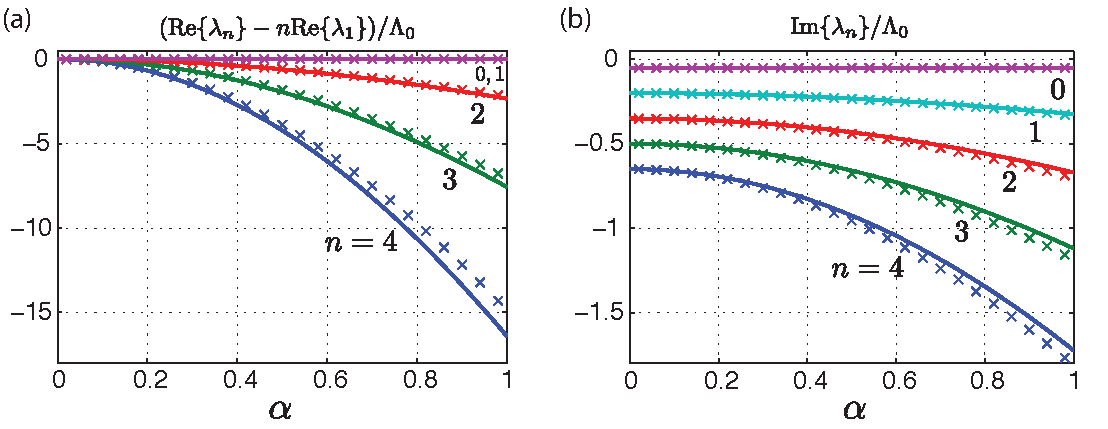
\includegraphics[width=1\textwidth]{./figs_Stannigel2012/Figure_suppl.pdf}
\caption
[Comparison of effective and exact description]
{Comparison of the effective analytic description
(Eqs.\,\eqref{eq:analytics}, lines) with exact eigenvalues of the Hamiltonian in
Eq.\,\eqref{eq:Hfull} (crosses) for different cavity field amplitudes $\alpha$.
All results are normalized to the scale
$\Lambda_0=g_0^4/(16\abs{\Delta_s}\delta^2)$ of the non-linearity.
(a) Deviation of the real parts of the eigenvalues from the result expected for
a linear oscillator, such that the splitting of the curves indicates an
effective non-linearity.
(b) Imaginary parts of the eigenvalues corresponding to decays. In both plots we
used the parameters $\Delta_s/g_0=-1$, $\delta/g_0=5$, $\kappa/g_0=2.5\times
10^{-2}$, $\gamma_m/g_0=2.5\times 10^{-4}$ and $N_{\rm th}=1$.}
\label{fig:numerics}
\end{figure}


To assess the validity of the effective phonon ME we now compare our result with
the dynamics of the full OMS.  Since we are mainly interested in the relation
between the phonon non-linearity and the corresponding dephasing and decay
rates, it is sufficient to evaluate the spectrum of the non-Hermitian
Hamiltonian, which  for the full model it is given by
\begin{equation}
\label{eq:Hfull}
\tilde H_{\rm full}=  H_{\rm lin}+ H_g - i\kappa c_s^\dag c_s - i\kappa
c_a^\dag c_a
 -i\frac{\gamma}{2} (N_{\rm th}+1) b^\dag b  -i\frac{\gamma}{2} N_{\rm th} b
b^\dag.
\end{equation}
In Fig.~\ref{fig:numerics} we plot the real and imaginary parts of the lowest
eigenvalues $\lambda_n$ of $\tilde H_{\rm full}$, which correspond to the lowest
number states $|n\rangle$ of the $B$ mode.
From the effective phonon model given in Eq.~\eqref{eq:SM_EffectiveME} and
\eqref{eq:SM_EffectiveME_corr} we obtain the approximate analytic results
\begin{subequations}
\label{eq:analytics}
\begin{equation}
{\rm Re} \{ \lambda_n\}= n \tilde \omega_m + n^2 \Lambda(n),
\end{equation}  
and
\begin{equation}
|{\rm Im} \{ \lambda_n\}|=\frac{\gamma}{2} N_{\rm th} + n \left(
\frac{\gamma}{2} (2N_{\rm th}+1) +\frac{\gamma^\prime}{2}\right) +n^2
\Gamma_\phi(n).
\end{equation}
\end{subequations}
We see a good agreement between these results for the effective model and the
exact numerics, both for the real and imaginary parts. Although there are some
deviations due to higher-order effects, the effective non-linear splitting
(Fig.~\ref{fig:numerics}(a)) is much larger than the induced decoherence
(Fig.~\ref{fig:numerics}(b)), as is expected for the chosen parameters. Hence,
we conclude that the effective model accurately describes the dynamics of the
mechanical resonator, and that the effective phonon non-linearity may serve as a
basis for gate operations as discussed in the main text and in the following
section.


\section{Phonon-phonon interactions} 

The derivation of the effective phonon nonlinearity, as outlined above for a
single resonator, can be easily adapted to two resonators as discussed in the
main text.
In this case we have 
\begin{equation}
H_0=  \sum_{i=1,2} \omega^i_m b_i^\dag b_i - \Delta_s c_s^\dag c_s - \Delta_a 
c_a^\dag c_a,
\end{equation}
and
\begin{equation}
H_g= \frac{g_0}{2} \left[c_a c_s^\dag (b^\dag_1-b_2^\dag) +    c_a^\dag c_s 
(b_1-b_2)\right].
\end{equation}
After changing into the displaced representation to eliminate the driving field
we obtain the linearized Hamiltonian
\begin{equation}
H_{\rm lin}�=  H_0  + \sqrt{2}\left( G(t)  c_a b_a^\dag + G^*(t) c_a^\dag
b_a\right),
\end{equation} 
where $b_a=(b_1-b_2)/\sqrt{2}$ and $G(t)=g_0\alpha(t)/2$.
For similar mechanical frequencies $\omega_m^1\simeq \omega_m^2=\omega_m$ the
symmetric resonator mode is decoupled and we can simply repeat the analysis from
above by identifying $b\equiv b_a$ and replacing $g_0$ by $\sqrt{2}g_0$.

For arbitrary $\omega_i$, we write the linear part of the Hamiltonian in its
diagonal form
\begin{equation}\label{eq:Hlin}
H_{\rm lin}�=  - \Delta_s c_s^\dag c_s -  \tilde \Delta_a  C^\dag C + \tilde
\omega_1 B_1^\dag B_1 + \tilde \omega_2 B_2^\dag B_2.
\end{equation} 
As in the single-resonator case the $c_s$ mode is unaffected,  but the $c_a$
mode now couples to both $b_1$ and $b_2$.  The resulting hybridized modes $C$,
$B_\pm$ depend on the choice of parameters $\omega_m^{1,2}, \Delta_a$ and $G$.
For the case of interest, i.e. for a symmetric detuning
$\omega_m^{1,2}=-\Delta_a \mp \delta$, we obtain
\begin{eqnarray}
C&=& \cos(2\Theta) c_a -  \sin(2\Theta)(B_1 + B_2)/\sqrt{2},\\
B_1&=& \cos^2(\Theta) b_1 + \sin(2\Theta) c_a/\sqrt{2} -  \sin^2(\Theta)b_2,\\
B_2&=& \cos^2(\Theta) b_2 + \sin(2\Theta) c_a/\sqrt{2} -  \sin^2(\Theta)b_1,
\end{eqnarray} 
where $\tan(2\Theta)=-\sqrt{2} |G|/\delta$. Therefore, for small $\Theta$ the
modes $B_{1,2}$ correspond to the original mechanical resonator modes $b_{1,2}$
and $\tilde \omega_i\approx \omega_m^{i}$.

As above, we can now re-express the dissipation and the non-linear coupling
$H_g$ in terms of $C$ and $B_\pm$. The modified mechanical dissipation terms are
given
\begin{equation}
\tilde{\mathcal{L}}_\gamma =  \sum_{i=1,2}  \frac{\gamma}{2}�\cos^2(2\Theta)
\mathcal{D}_{\rm th}[B_i] + \frac{\kappa}{2} \sin^2(2\Theta) \mathcal{D}[B_i],
\end{equation}
and for small $\Theta$ the optical decay rate $\gamma^\prime =\kappa
\sin^2(2\Theta)$ is the same as given above and in the main text.
Using the decomposition of the non-linear coupling as done in
Eq.~\eqref{eq:SM_HgDecomp},  we obtain
\begin{equation}
H_g^{(1)}= \frac{g_0}{\sqrt{8} }\sin(2\Theta)   \left( c_s+c_s^\dag\right)
\left(B_1^\dag B_1 - B^\dag_2 B_2\right),
\end{equation} 
the contribution $H_g^{(2)}$ vanishes and 
\begin{equation}
H_g^{\prime}= \frac{g_0}{2  }\cos(2\Theta)   \left( C c_s^\dag
(B_1^\dag-B_2^\dag) + {\rm H.c.}  \right).
\end{equation}
We see that the structure and also the relative frequency scales are identical
to the corresponding terms discussed for the single resonator above. Therefore,
under the same conditions we can eliminate the cavity mode and  obtain the
effective phonon master equation
\begin{equation}
\begin{split}
\dot \rho_m =& -i\left[\sum_i \tilde \omega_i B_i^\dag B_i + \Lambda (B_1^\dag
B_1-B_2^\dag B_2)^2 �, \rho_m \right]  \\
&+ \Gamma_\phi \mathcal{D}[(B_1^\dag B_1-B_2^\dag B_2)]\rho_m   +
\tilde{\mathcal{L}}_\gamma \rho_m.
\end{split} 
\end{equation}
 For small $\Theta$ this equation reduces to ME  (8) in the main text and
 higher-order corrections can be included in the same way as discussed for the
 single resonator case.

\chapter{Appendices for Chapter \ref{ch:Borregaard_PRL2015}}
\label{app:Borregaard_PRL2015}

This appendix describes the details of the
perturbation theory and the derivation of the effective Hamiltonian
$\hat{H}_{\text{eff}}$ and effective Lindblad operators. We describe the
situation both with and without a two-photon drive. Furthermore, we present the
results of a numerical simulation of the full dynamics of the gates to verify
the results found with perturbation theory and address the question of how
strong a drive we can allow for. In the end, this determines the gate time as
described in the article. Finally we discuss of the additional errors described
in the final part of the article.

\section{Perturbation theory}

We will now give the details of the perturbation theory and the derivation of
the effective operators together with the success probabilitites, gate times and
gate errors (see \tabref{tab:table1}). Our perturbation theory is based on the
effective operator formalism described in Ref.~\cite{Florentin}.
 
\begin{table} [h]
\centering
\begin{tabular}{|c|c|c|c|c|}
\hline
Gate & Origin of error & Error & Probability & Time  \\ \hline CZ-gate &
\specialcell{$\gamma_{g}=0$
\\$\gamma_{g}>0$} & \specialcell{$0$\\$\sim
\frac{\gamma_{g}}{\gamma\sqrt{C}}$} & $\sim 1-\frac{6}{\sqrt{C}}$ &
$\sim\frac{15\pi\sqrt{C}\gamma}{2\Omega^{2}}$\\ \hline Toffoli &
\specialcell{$\Gamma_{i}\neq\Gamma_{j}$\\$\gamma_{g}>0$} &
\specialcell{$\lesssim\!\frac{0.3}{C}\quad$\\$\sim\!\!
\frac{\gamma_{g}}{\gamma\sqrt{C}}$} & $\sim 1-\frac{3}{\sqrt{C}}$ &
$\sim\frac{4\pi\sqrt{C}\gamma}{\Omega^{2}}$ \\ \hline
\end{tabular}
\caption
[Comparison of CZ and Toffoli gates]
{The errors, success probabilities and gate times of the $N$-qubit
Toffoli gate and the $CZ$-gate considered in the article. Note that the
branching fraction $\gamma_{g}/\gamma$ can be made arbitrarily small using a far
detuned two-photon driving as explained in below. $\Gamma_{i}$ is the rate of
detectable errors for the qubit state with $i$ qubits in state $\ket{1}$. The
success probability of the CZ-gate can be increased at the expense of an error
scaling of $1/C$ as explained in the article.}
\label{tab:table1}
\end{table}  

First, we treat the simplest situation where the auxiliary atom is directly
driven to an excited state $\ket{E}$ by a weak classical drive $\Omega$ as shown
in \reffig{fig:figureS1} (reproduced from Fig. 1 in the article). Note that we
allow for some decay from $\ket{E}\to\ket{g}$ with decay rate $\gamma_{g}$ as
opposed to the situation in the article. We will later consider the situation
where this decay rate is suppressed using a two-photon drive. The level
structure of the qubit atoms are also shown in \reffig{fig:figureS1}.

\begin{figure} [H]
\centering
\includegraphics[width=0.35\textwidth]{./figs_Borregaard_PRL2015/figureS1a}
\includegraphics[width=0.35\textwidth]{./figs_Borregaard_PRL2015/figureS1b}
\caption
[Level structure of qubit an auxiliary atoms]
{(a) Level structure of the qubit atoms. Only state $\ket{1}$ couples
to the cavity and we assume that the excited level decays to some level
$\ket{\tilde{o}}$, possible identical to $\ket{f}$ or $\ket{0}$. (b) Level
structure of the auxiliary atom and the transitions driven by the weak laser
($\Omega$) and the cavity ($g_{f}$). We allow for some decay from
$\ket{E}\to\ket{g}$ with decay rate $\gamma_{g}$. }
\label{fig:figureS1}
\end{figure}

The Hamilton describing the system in a proper rotating frame is given by Eqs.
(1)-(3) in the article and is reproduced here
\begin{eqnarray} \label{eq:hamil1}
\hat{H}&=&\hat{H}_{e}+\hat{V}+\hat{V}^{\dagger}, \\
\hat{H}_{e}&=&\Delta_{E}\ket{E}\bra{E}+g_{f}(\hat{a}\ket{E}\bra{f}+H.c) \nonumber \\
&&+\sum_{k}\Delta_{e}\ket{e}_{k}\bra{e}+g(\hat{a}\ket{e}_{k}\bra{1}+H.c), \\
\hat{V}&=&\frac{\Omega}{2}\ket{E}\bra{g},
\end{eqnarray}          
where we have assumed for simplicty that all couplings ($g,\Omega$) are real and
$k$ labels the qubit atoms ($\hbar=1$). We have defined
$\Delta_{E}=\omega_{E}-\omega_{g}-\omega_{L}$, and
$\Delta_{e}=\omega_{e}-\omega_{g}-\omega_{L}+\omega_{f}-\omega_{1}$ where
$\omega_{L}$ is the laser frequency and otherwise $\omega_{x}$ is the frequency
associated with level $x$. Note that we assume the cavity frequency to be
$\omega_{c}=\omega_{L}+\omega_{g}-\omega_{f}$ such that we are on resonance with
the $\ket{g}\to\ket{E}\to\ket{f}$ two-photon transition.

The dissipation in the system is assumed to be described by Lindblad operators
such that $\hat{L}_{0}=\sqrt{\kappa}\hat{a}$ describes the cavity decay with
decay rate $\kappa$, $\hat{L}_{g}=\sqrt{\gamma_{g}}\ket{g}\bra{E}$, and
$\hat{L}_{f}=\sqrt{\gamma_{f}}\ket{f}\bra{E}$ describes the decay of the
auxiliary atom and $\hat{L}_{k}=\sqrt{\gamma}\ket{\tilde{o}}_{i}\bra{e}$
describes the decay of the qubit atoms ($k=1,2\ldots N$). As described in the
article $\ket{\tilde{o}}$ may or may not coincide with $\ket{0}$ or $\ket{1}$.
Assuming that $\Omega$ is weak ($\Omega^{2}/\Delta_{E}\ll\Delta_{E}$ and
$\Omega\ll g$), we can treat the driving as a perturbation to the system. As
shown in Ref.~\cite{Florentin}, the dynamics of the system is then governed by
an effective master equation of the form
\begin{equation}
\dot{\rho}=i\left[\rho,\hat{H}_{\text{eff}}\right] +
\sum_{x}\hat{L}_{x}^{\text{eff}}\rho(\hat{L}_{x}^{\text{eff}})^{\dagger}-\frac{1}{2}\left((\hat{L}_{x}^{\text{eff}})^{\dagger}\hat{L}_{x}^{\text{eff}}\rho+\rho(\hat{L}_{x}^{\text{eff}})^{\dagger}\hat{L}_{x}^{\text{eff}}\right),
\end{equation}
where $\rho$ is the density matrix of the system, $\hat{H}_{\text{eff}}$ is an
effective Hamiltonian, and  $L_{x}^{\text{eff}}$ are effective Lindblad
operators with $x=0,g,f,k$.  The effective operators are found from:
\begin{eqnarray} \label{eq:supheff1}
\hat{H}_{\text{eff}}&=&-\frac{1}{2}\hat{V}^{\dagger}\left(\hat{H}_{\text{NH}}^{-1}+(\hat{H}_{\text{NH}}^{-1})^{\dagger}\right)\hat{V}
\\
\hat{L}_{x}^{\text{eff}}&=&\hat{L}_{x}\hat{H}_{\text{NH}}^{-1}\hat{V},  \label{eq:supleff1}
\end{eqnarray}
where 
\begin{equation}
\hat{H}_{\text{NH}}=\hat{H}_{e}-\frac{i}{2}\sum_{x}\hat{L}_{x}^{\dagger}\hat{L}_{x},
\end{equation}
is the no-jump Hamiltonian. The Hilbert space of the effective operators can be
described in the basis of $\left\{\ket{g},\ket{f}\right\}$ of the auxiliary atom
and the states $\left\{\ket{0},\ket{1},\ket{\tilde{o}}\right\}$ of the qubit
atoms. To ease the notation, we define the projection operators $\hat{P}_{n}$
which projects on to the states with $n$ qubits in state $\ket{1}$. From
Eq.~\eqref{eq:supheff1} and \eqref{eq:supleff1} we then find:
\begin{eqnarray}
\hat{H}_{\text{eff}}&=&\sum_{n=0}^{N}\frac{-\Omega^{2}}{4\gamma}\mathrm{Re}\left\{\frac{i\tilde{\Delta}_{e}/2+nC}{\tilde{\Delta}_{e}(i\tilde{\Delta}_{E}/2+C_{f})+\tilde{\Delta}_{E}nC}\right\}\ket{g}\bra{g}\otimes \hat{P}_{n} \nonumber \\
&=&\sum_{n=0}^{N}\Delta_{n}\ket{g}\bra{g}\otimes \hat{P}_{n}
\label{eq:supham2}\\
\hat{L}_{0}^{\text{eff}}&=&\sum_{n=0}^{N}\frac{1}{2\sqrt{\gamma}}\frac{\sqrt{C_{f}}\tilde{\Delta}_{e}\Omega}{\tilde{\Delta}_{e}(i\tilde{\Delta}_{E}/2+C_{f})+n\tilde{\Delta}_{E}C}\ket{f}\bra{g}\otimes
\hat{P}_{n} \nonumber \\
&=&\sum_{n=0}^{N}r_{0,n}^{\text{eff}}\ket{f}\bra{g}\otimes \hat{P}_{n}
\label{eq:subleff1} \\
\hat{L}_{g}^{\text{eff}}&=&\sum_{n=0}^{N}\frac{1}{2}\frac{(i\tilde{\Delta}_{e}/2+nC)\Omega}{\tilde{\Delta}_{e}(i\tilde{\Delta}_{E}/2+C_{f})+n\tilde{\Delta}_{E}C}\frac{\sqrt{\gamma_{g}}}{\gamma}\ket{g}\bra{g}\otimes
\hat{P}_{n} \nonumber \\
&=&\sum_{n=0}^{N}r_{g,n}^{\text{eff}}\ket{g}\bra{g}\otimes \hat{P}_{n} \\
\hat{L}_{f}^{\text{eff}}&=&\sum_{n=0}^{N}\frac{1}{2}\frac{(i\tilde{\Delta}_{e}/2+nC)\Omega}{\tilde{\Delta}_{e}(i\tilde{\Delta}_{E}/2+C_{f})+n\tilde{\Delta}_{E}C}\frac{\sqrt{\gamma_{f}}}{\gamma}\ket{f}\bra{g}\otimes
\hat{P}_{n} \nonumber \\
&=&\sum_{n=0}^{N}r_{f,n}^{\text{eff}}\ket{f}\bra{g}\otimes \hat{P}_{n} \\
\hat{L}_{k}^{\text{eff}}&=&\sum_{n=1}^{N}-\frac{1}{2\sqrt{\gamma}}\frac{\sqrt{C_{f}}\sqrt{C}\Omega}{\tilde{\Delta}_{e}(i\tilde{\Delta}_{E}/2+C_{f})+n\tilde{\Delta}_{E}C}\ket{f}\bra{g}\otimes\ket{\tilde{o}}_{k}\bra{1}\otimes\hat{P}_{n}
\nonumber \\
&=&\sum_{n=1}^{N}r_{n}^{\text{eff}}\ket{f}\bra{g}\otimes\ket{\tilde{o}}_{k}\bra{1}\otimes\hat{P}_{n},
\label{eq:subleff2}
\end{eqnarray}
where we have defined the cooperativities $C_{(f)}=g_{(f)}^{2}/\gamma\kappa$ for
the qubit (auxiliary) atoms and the complex detunings
$\tilde{\Delta}_{E}\gamma=\Delta_{E}-i\gamma_{f}/2$ and 
$\tilde{\Delta}_{e}\gamma=\Delta_{e}-i\gamma/2$. Note that we have defined the
parameters $r^{\text{eff}}_{0,n}, r^{\text{eff}}_{g,n},r^{\text{eff}}_{f,n}$ and
$r_{n}^{\text{eff}}$ in Eqs. \eqref{eq:subleff1}-\eqref{eq:subleff2} to
characterize the decays described by the Lindblad operators. Note that
$r_{0}^{\text{eff}}=0$. In our calculations we parametrize the difference
between the auxiliary atom and the qubit atoms by $C_{f}=\alpha C$ and
$\gamma_{f}=\beta\gamma$ to easier treat the limit of $C\gg1$ that we are
interested in.

\subsection{Success probability and fidelity}
Eqs. \eqref{eq:subleff1}-\eqref{eq:subleff2} show that the effect of all
Lindblad operators, except $\hat{L}_{g}^{\text{eff}}$, is that the state of the
auxiliary atom is left in state $\ket{f}$. All these errors are thus detectable
by measuring the state of the auxiliary atom at the end of the gate. For the
heralded gates where we condition on measuring the auxiliary atom in state
$\ket{g}$ at the end of the gates, these detectable decays therefore do not
effect the fidelity of the gates but only the success probability.  The rate
$\Gamma_{n}$ of the detectable decays for a state with $n$ qubits in state
$\ket{1}$ is
$\Gamma_{n}=\abs{r_{0,n}^{\text{eff}}}^{2}+\abs{r_{f,n}^{\text{eff}}}^{2}+\abs{r_{n}^{\text{eff}}}^{2}$
and assuming an initial qubit state described by density matrix $\rho_{qubit}$
the success probability of the gates is
\begin{equation}
P_{\text{success}}=
\sum_{n=0}^{N}\text{Tr}
\left\{e^{-\Gamma_{n}t_{\text{gate}}}\rho_{\text{qubit}}\hat{P}_{n}\right\},
\end{equation}
where $t_{\text{gate}}$ is the gate time and $\text{Tr}$ denotes the trace. 

Having removed the detrimental effect of the detectable errors by heralding on a
measurement of the auxiliary atom the fidelity of the gates will be determined
by more subtle, undetectable errors (see below). We define the fidelity, $F$ of
the gate as
\begin{equation}
F=\frac{1}{P_{\text{success}}}\bra{\psi}\bra{g}
\tilde{\rho}_{\text{qubit}}\ket{g}\ket{\psi},
\end{equation} 
where we have assumed that the ideal qubit state after the gate is a pure state
$\ket{\psi}$ and $\tilde{\rho}_{qubit}$ is the actual density matrix of the
qubits and the auxiliary atom after the gate operation.

\subsection{$N$-qubit Toffoli gate}

As shown in the article, the effective Hamiltonian in Eq.~\eqref{eq:supham2} is
sufficient to make a Toffoli gate by putting the qubit atoms on resonance
($\Delta_{e}=0$). We will now treat the worst case and average fidelities of the
general Toffoli gate referred to in the article. The undetectable errors
limiting the fidelities are the following.
\begin{itemize}
\item As described in the article the energy shifts of the coupled qubit states
are all $\Delta_{n>0}\sim\Omega^{2}/(4\gamma\sqrt{C})$ in the limit $C\gg1$.
However, to higher order in $C$, we find corrections on the order
$\mathcal{O}(\Omega^{2}/C^{3/2})$ to the energy shifts, which depend on the
number of qubits that couples. The gate time of the Toffoli gate is
$t_{\text{T}}\sim4\pi\sqrt{C}\gamma/\Omega^{2}$ and consequently, the higher
order corrections give uneven phase shifts on the order of $\mathcal{O}(C^{-1})$
for the coupled qubit states at the end of the gate. This leads to a phase error
in the fidelity of $\mathcal{O}(C^{-2})$.
\item The difference between the rates of detectable errors ($\Gamma_{n}$) for
different qubit states changes the relative weight of the qubit states during
the gate. This error wil be $\mathcal{O}(C^{-1})$ as shown below.
\item For $\gamma_{g}>0$ the undetectable decay from $\ket{E}\to\ket{g}$ in the
auxiliary atom will destroy the coherence between the qubit states. We find that
this error will be $\sim \frac{\gamma_{g}}{\gamma\sqrt{C}}$. For now, we will
assume that $\gamma_{g}=0$ and thus ignore this error since we will show that we
can suppress the branching fraction $\gamma_{g}/\gamma$ arbitrary close to zero
by having a two photon driving.
\end{itemize}  

Assuming that $\gamma_{g}=0$, the dominating source of error limiting the
performance of the Toffoli gate is thus the difference between the rates of the
detectable errors for the qubit states. We tune $\Delta_{E}$ such that
$\Gamma_{0}=\Gamma_{1}$ and the largest difference between the detectable errors
is thus between the completely uncoupled state and the state with all qubit
atoms in state $\ket{1}$. As a result, we can find an upper bound on the
fidelity of the $N$ qubit Toffoli gate, considering an initial state
$\ket{0}^{\otimes N}+\ket{1}^{\otimes N}$ in the limit $N\to\infty$ because this
state experiences the largest difference between the number of coupled and
uncoupled qubits. We find that the upper bound on the fidelity and the
corresponding success probability is
\begin{eqnarray}
F_{\text{up}}&\sim&1-\frac{\pi^{2}\alpha}{16(\alpha+\beta)}\frac{1}{C}\\
P_{\text{success,up}}&\sim&1-
\frac{(\alpha+2\beta)\pi}{2\sqrt{\alpha}\sqrt{\alpha+\beta}} \frac{1}{\sqrt{C}}.
\end{eqnarray}.   
In general, the fidelity of the gate will, however, be larger than what is
suggested above. Considering a generic input state  $(\ket{0}+\ket{1})^{\otimes
N}$ with the same parameters as above, we find
\begin{eqnarray}
F_{\text{gen}}&\sim&1-k(N)\frac{\alpha \pi^{2}}{\alpha+\beta}\frac{1}{C} \\
P_{\text{success,gen}}&\sim&1-\frac{(d(N)\alpha+2\beta)\pi}{2\sqrt{\alpha}\sqrt{\alpha+\beta}}
\frac{1}{\sqrt{C}},
\end{eqnarray}
where $k(N),d(N)$ are scaling factors which depend on the number of qubits $N$.
We calculate $k(N)$ and $d(N)$ numerically for $N=1-100$ using the perturbation
theory and find that that they both decrease with $N$ (see
\reffig{fig:toffoli}). The upper bounded and generic fidelities and
corresponding success probabilities are shown in \reffig{fig:toffoli} for
different number of qubits, $N$.
\begin{figure} 
\centering
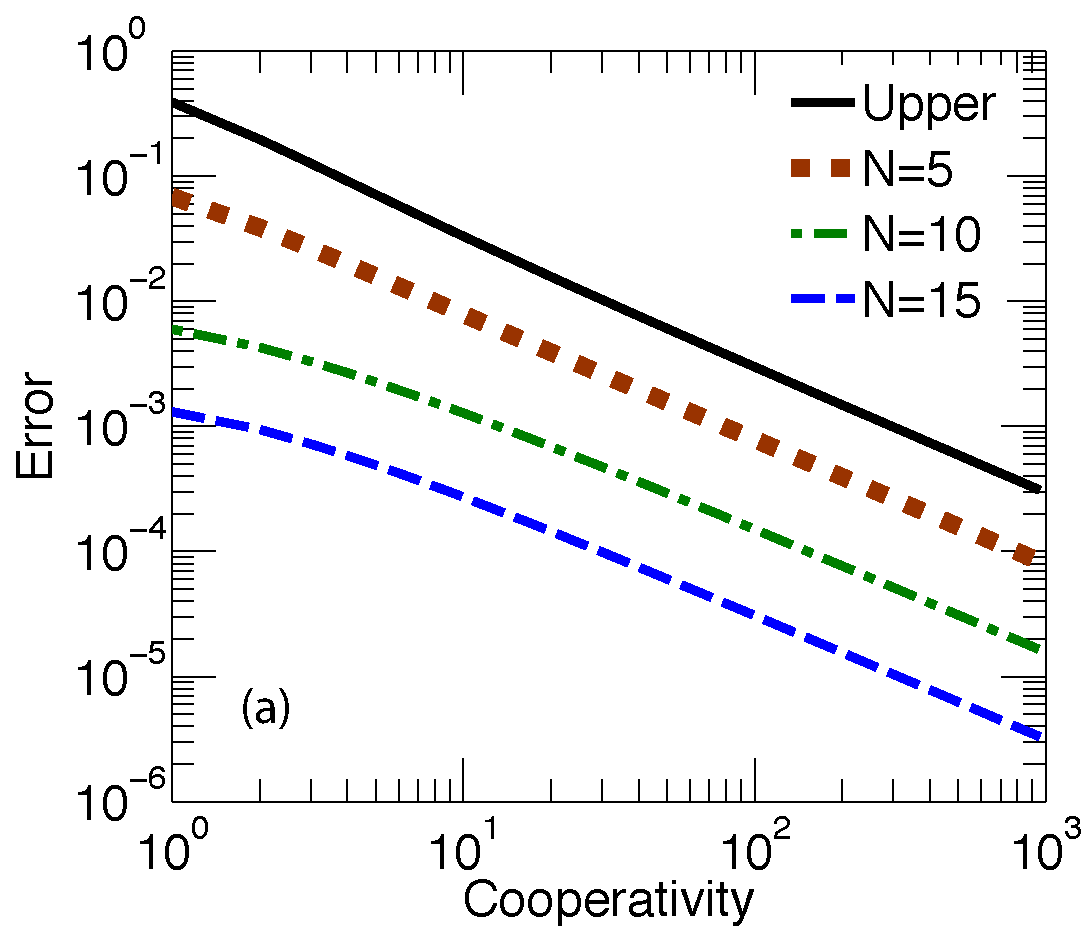
\includegraphics[width=0.46\textwidth]{./figs_Borregaard_PRL2015/figure2a}
\quad\quad
\includegraphics[width=0.46\textwidth]{./figs_Borregaard_PRL2015/figure2b}
\caption
[Error and success probability vs cooperativity]
{(a) Gate error of the Toffoli for different initial states as a
function of cooperativity. We have plotted the generic error for $N=5,10$, and 15 and the upper bound of the error. Note that the generic error decreases as $N$ increases. We have fixed $\Delta$ such that $\Gamma_{0}=\Gamma_{1}$ and have assumed that $\alpha=\beta=1$. (b) The failure probabilities $1-P_{\text{success,up}}$ and  $1-P_{\text{success,gen}}$ as a function of cooperativity. $1-P_{\text{success,gen}}$ is plotted for $N=5,10,15$. We have used the same assumptions as in (a). In general, the failure probability only have a weak dependence on $N$. Note that the line for $1-P_{\text{success, gen}},N=5$ coincides with  $1-P_{\text{success,up}}$.}
\label{fig:toffoli}
\end{figure}
As $N$ increases we obtain higher generic fidelity, whereas the success
probability is almost independent of $N$.

\subsection{CZ-gate}

In the special case of only two qubits the Toffoli gate is referred to as a
control-phase (CZ) gate. As shown in the article, we can, in this case,
completely remove the errors from the gate by choosing the detunings
$\Delta_{E}$ and $\Delta_{e}$ such that $\Gamma_{0}=\Gamma_{1}=\Gamma_{2}$ and
combining it with single qubit rotations we can ensure the right phase
evolution. In the general case where $\alpha,\beta\neq1$, the detunings
$\Delta_{e}$ and $\Delta_{E}$ are
\begin{eqnarray}
\Delta_{E}&=&\frac{\gamma}{2}\sqrt{\beta}\sqrt{4\alpha C+\beta} \\
\Delta_{e}&=&\frac{\alpha C\gamma^{2}}{2\Delta_{E}}. 
\end{eqnarray}
The success probability of the gate is then
\begin{equation}
P_{\text{success}}\simeq1-\pi\frac{8\beta^{2}+6\beta\alpha+\alpha^{2}}{8\beta^{3/2}\sqrt{\alpha}}\frac{1}{\sqrt{C}},
\end{equation} 
and we find that the gate time is
$t_{\text{CZ}}\simeq\frac{\gamma\pi\sqrt{\alpha}(\alpha+2\beta)(\alpha+4\beta)}{2\beta^{3/2}\Omega^{2}}\sqrt{C}$
in the limit $C\gg1$.
\subsection{Two-photon driving}

We now describe the details of the implementation where the auxiliary atoms is
driven by a two-photon process as shown in \reffig{fig:figureS2} (reproduced
from Fig. 4(a) in the article) in order to suppress the dominant undetectable
error caused by spontaneous decay of the auxilliary atom into the state
$\ket{g}$ ($\hat{L}_{g}$).

\begin{figure}
\centering
\includegraphics[width=0.7\textwidth]{./figs_Borregaard_PRL2015/figureS2} 
\caption
[Levels structure of auxiliary atom]
{(a) Level structure of the auxiliary atom and the transitions driven by
a weak laser ($\Omega$), a microwave field ($\Omega_{\text{MW}}$) and the cavity
($g_{f}$). We assume that $\ket{E}\leftrightarrow\ket{f}$ is a closed transition
and for simplicity we also assume that $\ket{E_{2}}\leftrightarrow\ket{g}$ is a
closed transition but this is not a necessity. The figure also indicates how the
levels could be realized in ${}^{87}$Rb. Here $\ket{r^{(e)},r^{(e)}}$ with
$r=1,2,3$ refers to state $\ket{\text{F}^{(e)}=r,\text{m}_{\text{F}}^{(e)}=r}$
in $5^{2}S_{1/2}$ $(5^{2}P_{3/2})$. (b) Effective three level atom realized by
mapping the two-photon drive to an effective decay rate $\tilde{\gamma}_{g}$ and
an effective drive $\tilde{\Omega}$}
\label{fig:figureS2}
\end{figure} 

The Hamiltonian in a proper rotating frame is
\begin{eqnarray} \label{eq:supphamil2}
\hat{H}&=&\hat{H}_{e}+\hat{V}+\hat{V}^{\dagger}, \\
\hat{H}_{e}&=&\Delta_{E}\ket{E}\bra{E}+\Delta_{E2}\ket{E_{2}}\bra{E_{2}}+g_{f}(\hat{a}\ket{E}\bra{f}+H.c)
\nonumber \\
&&+\frac{\Omega_{\text{MW}}}{2}(\ket{E}\bra{E_{2}}+H.c.) \nonumber \\
&&+\sum_{k}\Delta_{e}\ket{e}_{k}\bra{e}+g(\hat{a}\ket{e}_{k}\bra{1}+H.c.), \\
\hat{V}&=&\frac{\Omega}{2}\ket{E_{2}}\bra{g},
\end{eqnarray}  
where we have now defined
$\Delta_{E}=\omega_{E}-\omega_{g}-\omega_{laser}-\omega_{\text{MW}}$, 
$\Delta_{E2}=\omega_{E2}-\omega_{g}-\omega_{laser}$ and
$\Delta_{e}=\omega_{e}-\omega_{g}-\omega_{laser}-\omega_{\text{MW}}+\omega_{f}-\omega_{1}$.
Here $\omega_{laser}$ is the frequency of the laser drive ($\Omega$),
$\omega_{\text{MW}}$ is the frequency of the microwave field
($\Omega_{\text{MW}}$) and otherwise $\omega_{x}$ is the frequency associated
with level $x$. We assume that the frequency of the cavity is
$\omega_{c}=\omega_{laser}+\omega_{\text{MW}}+\omega_{g}-\omega_{f}$ such that
the three photon Raman transition from $\ket{g}\to\ket{f}$ is resonant. We have
assumed that $\Delta_{E2}$ is large and positive such that the rotating wave
approximation is valid for the microwave field.
The Lindblad operators describing the system are the same as described below
Eq.~\eqref{eq:hamil1} except that
$\hat{L}_{g}\to\sqrt{\gamma_{g}}\ket{g}\bra{E_{2}}$. Assuming a weak drive
$\Omega$, we can follow the same recipe as before to find the following
effective operators describing the dynamics of the system.
\bal
&&\hat{H}^{(2)}_{\text{eff}}
= \sum_{n=0}^{N}\Delta^{(2)}_{n}\ket{g}\bra{g} \otimes \hat{P}_{n}
\label{eq:supham3}\\
&&\qquad \Delta^{(2)}_{n} = \frac{-\Omega^{2}}{4\gamma}\mathrm{Re}
\left[\frac{\tilde{\Delta}_{e}(i\tilde{\Delta}_{E}/2+C_{f})+n
\tilde{\Delta}_{E}C}{\tilde{\Delta}_{E2}\tilde{\Delta}_{e}
(i\tilde{\Delta}_{E}/2+C_{f})+n\tilde{\Delta}_{E}\tilde{\Delta}_{E2}
C-i\tilde{\Delta}_{e}\tilde{\Omega}_{\text{MW}}^{2}/8-n
\tilde{\Omega}_{\text{MW}}^{2}C/4}\right]\nonumber
\\
&&\hat{L}_{0}^{\text{eff}(2)}=\sum_{n=0}^{N}r_{0,n}^{\text{eff}(2)}\ket{f}\bra{g}\otimes
\hat{P}_{n}
\label{eq:subleff3}\\
&&\qquad r_{0,n}^{\text{eff}(2)} =
\frac{-1}{4\sqrt{\gamma}}\frac{\sqrt{C_{f}}\tilde{\Delta}_{e}\Omega\tilde{\Omega}_{\text{MW}}}{\tilde{\Delta}_{E2}\tilde{\Delta}_{e}(i\tilde{\Delta}_{E}/2+C_{f})+n\tilde{\Delta}_{E2}\tilde{\Delta}_{E}C-i\tilde{\Delta}_{e}\tilde{\Omega}_{\text{MW}}^{2}/8-n\tilde{\Omega}_{\text{MW}}^{2}C/4}
\nonumber
\\
&&\hat{L}_{g}^{\text{eff}(2)}=\sum_{n=0}^{N}r_{g,n}^{\text{eff}(2)}\ket{g}\bra{g}\otimes
\hat{P}_{n}\\
&&\qquad r_{g,n}^{\text{eff}(2)} =
\frac{\Omega}{2}\frac{\tilde{\Delta}_{e}(i\tilde{\Delta}_{E}/2+C_{f})+n\tilde{\Delta}_{E}C}{\tilde{\Delta}_{E2}\tilde{\Delta}_{e}(i\tilde{\Delta}_{E}/2+C_{f})+n\tilde{\Delta}_{E2}\tilde{\Delta}_{E}C-i\tilde{\Delta}_{e}\tilde{\Omega}_{\text{MW}}^{2}/8-n\tilde{\Omega}_{\text{MW}}^{2}C/4}\frac{\sqrt{\gamma_{g}}}{\gamma}
\nonumber
\\
&&\hat{L}_{f}^{\text{eff}(2)} =
\sum_{n=0}^{N}r_{f,n}^{\text{eff}(2)}\ket{f}\bra{g} \otimes \hat{P}_{n}\\
&&\qquad r_{f,n}^{\text{eff}(2)} = 
-\frac{\Omega}{4}\frac{(i\tilde{\Delta}_{e}/2+nC)\tilde{\Omega}_{\text{MW}}}{\tilde{\Delta}_{E2}\tilde{\Delta}_{e}(i\tilde{\Delta}_{E}/2+C_{f})+n\tilde{\Delta}_{E2}\tilde{\Delta}_{E}C-i\tilde{\Delta}_{e}\tilde{\Omega}_{\text{MW}}^{2}/8-n\tilde{\Omega}_{\text{MW}}^{2}C/4}\frac{\sqrt{\gamma_{f}}}{\gamma}
\nonumber
\eal
\bal
&&\hat{L}_{k}^{\text{eff}(2)} =
\sum_{n=0}^{N-1}r_{n}^{\text{eff}(2)}\ket{f}\bra{g}\otimes\ket{\tilde{o}}_{k}\bra{1}\otimes
\hat{P}_{n}, \label{eq:subleff4} \\
&&\qquad r_{n}^{\text{eff}(2)} = 
\frac{1}{4\sqrt{\gamma}}\frac{\sqrt{C_{f}}\sqrt{C}\tilde{\Omega}_{\text{MW}}\Omega}{\tilde{\Delta}_{E2}\tilde{\Delta}_{e}(i\tilde{\Delta}_{E}/2+C_{f})+n\tilde{\Delta}_{E2}\tilde{\Delta}_{E}C-i\tilde{\Delta}_{e}\tilde{\Omega}_{\text{MW}}^{2}/8-n\tilde{\Omega}_{\text{MW}}^{2}C/4}
\nonumber
\eal
where we have defined the complex detuning
$\tilde{\Delta}_{E2}\gamma=\Delta_{E2}-i\gamma_{g}/2$ and the parameters
$r_{0,n}^{\text{eff}(2)},r_{g,n}^{\text{eff}(2)},r_{f,n}^{\text{eff}(2)}$ and
$r_{n}^{\text{eff}(2)}$ to characterize the decay described by the Lindblad
operators.

We are interested in the limit of large detuning $\Delta_{E2}$ and large
cooperativity $C$. In this limit, we find that the dynamics of the system can be
mapped to a simple three level atom with effective driving
$\tilde{\Omega}\sim\Omega\Omega_{\text{MW}}/(2\Delta_{E2})$ and an effective
decay $\tilde{\gamma}_{g}\sim\gamma_{g}\Omega_{\text{MW}}^{2}/\Delta_{E2}^{2}$
as shown in \reffig{fig:figureS2}. In principle, the effective operator
$\hat{L}_{0}^{\text{eff}(2)}$ leads to an effective decay rate of
$\tilde{\gamma}=\gamma_{g}\Omega^{2}/\Delta_{E2}^{2}$ to lowest order in $C$ 
but we find that this first order term do not destroy the coherence between the
qubit states since it is independent of $n$. There is, therefore, no effect of
these scattering events and the performance of the gate behaves as if there is
an effective decay rate of
$\tilde{\gamma}_{g}\sim\gamma_{g}\Omega_{\text{MW}}^{2}/\Delta_{E2}^{2}$. Note
that we also have an AC stark shift imposed on the level $\ket{g}$ by the laser
characterized by $\Omega$. This will give an overall phase to the system,
$\sim\Omega^{2}/(4\Delta_{E2})t$, which we can neglect since it does not
influence the gates.
Since we can do the mapping to the simple three level atom, we find similar
results for the performance of the gates for the two-photon scheme as for the
simple three level scheme only with effective decay $\tilde{\gamma}_{g}$ and
drive $\tilde{\Omega}$ given by the two-photon process. Note, however, that we
now assume $\gamma_{g}>0$, which introduces an undetectable error as previously
mentioned. We find that this introduces an error in the fidelity of both gates
of roughly
\begin{eqnarray}
&\sim&\frac{(\alpha^{2}-4\alpha\beta-6\beta^{2})\pi^{2}}{128\beta^{2}}\frac{\gamma_{g}^{4}}{\gamma^{4}\Delta_{E2}^{4}}+\frac{(\alpha^{2}+4\alpha\beta+6\beta^{2})\pi}{16\sqrt{\alpha\beta}(\alpha+2\beta)(\alpha+5\beta))}\frac{\gamma_{g}\Omega_{\text{MW}}^{2}}{\gamma\Delta_{E2}^{2}}\frac{1}{\sqrt{C}}\qquad.
\end{eqnarray}  
Nonetheless, this error can be suppressed arbitrarily much be increasing
$\Delta_{E2}$, which enable us to have a heralded CZ-gate with arbitrarily small
error in a realistic atomic setup using the two-photon drive.

\section{Gate time}
Here we address the question of how strongly we can drive the system and still
maintain the validity of perturbation theory. We need to adress this question
since the gate time depends inversely on the driving strength as shown in the
article and hence this limits the achievable gate time. A necessary criterion
for our pertubation theory to be valid is that the energy shifts $\Delta_{n}$
(see Eq.~\eqref{eq:supham2} and Eq.~\eqref{eq:supham3}) are small compared to
the driving, i.e. $\sim\Delta_{n}^{2}/\Omega^{2}\ll1$. From
Eq.~\eqref{eq:supham2} we find that
$\Delta_{n}^{2}/\Omega^{2}\sim\Omega^{2}/(16\Delta_{E}^{2})$ to leading order in
the cooperativity $C$ and this criterion is therefore met for
$\Omega\ll4\Delta_{E}$. Similarly, for the two-photon process, we find from
Eq.~\eqref{eq:supham3} that
$(\Delta_{n}^{(2)})^{2}/\Omega^{2}\sim\Omega^{2}/(16\Delta_{E2}^{2})$, to
leading order in $C$. Here we thus need $\Omega\ll4\Delta_{E2}$.

Another criterion need to be meet in order for our perturbative theory to be
valid. If none of the qubits couple, we are effectively driving the auxiliary
atom/cavity system into a dark state of the form
$\cos(\theta)\ket{0,g}-\sin(\theta)\ket{1,f}$, where the mixing angle is
$\theta\sim\Omega/g$. Here the number refers to the number of cavity photons. To
adiabatically eliminate the state $\ket{f,1}$ from the Hamiltonian as we have
done in the effective Hamiltonian requires that $\Omega/g\ll1$. Mapping this
criterion to the effective three level scheme realized in the two-photon scheme
gives $\Omega\Omega_{\text{MW}}/(2\Delta_{E2}g)\ll1$.

Finally, we need to consider the scattering of photons from the level $\ket{E2}$
in the two-photon scheme. If the number of scattering events, $n_{scat}$ is
large compared to $\Omega^{2}/(16\Delta_{E2}^{2})$, the perturbation theory is
not valid even though the other criterions are met. We find that
$n_{scat}\sim\frac{12\sqrt{C}\gamma^{2}}{\Omega_{\text{MW}}^{2}}$ for the
CZ-gate and we thus need to have 
$\frac{3\sqrt{C}\gamma^{2}\Omega^{2}}{\Delta_{E2}^{2}\Omega_{\text{MW}}^{2}}\ll1$

The different criterions for the validity of the perturbation theory are
summarized in \tabref{tab:tableS1}.
\begin{table} [H]
\centering
\begin{tabular}{|c|c|}
\hline
Simple scheme & Two-photon scheme  \\ \hline
$\Omega/(4\Delta_{E})\ll1$ & $\Omega/(4\Delta_{E2})\ll1$ \\ \hline
$\Omega/g\ll1$ & $\Omega\Omega_{\text{MW}}/(\Delta_{E2}g)\ll1$ \\ \hline
- & $3\sqrt{C}\gamma^{2}\Omega^{2}/(\Delta_{E2}^{2}\Omega_{\text{MW}}^{2})\ll1$  \\ \hline
\end{tabular}
\caption
[Perturbation validity criteria]
{The criterions for our perturbation theory to be valid. }
\label{tab:tableS1}
\end{table}
For all the gate schemes, we have assumed that
$\Delta_{E}\propto\sqrt{C}\gamma$. The first criterion for the simple scheme
(see \tabref{tab:tableS1}) can thus be met with a driving of
$\Omega=a\gamma\sqrt{C}$ where $a/4\ll1$. This driving results in a gate time
that decreases as $1/\sqrt{C}$. The value of $a$ will determine the size of the
non-adiabatic error. The second criterion is also fulfilled for this driving as
long as $\sqrt{\gamma/\kappa}\ll1$. In realistic systems such as the nanocavity
system described in Ref.~\cite{thompson, Tiecke}, the ratio $\kappa/\gamma$ can
be on the order of 100-1000.
For the two-photon scheme, we find from \tabref{tab:tableS1} that we can choose
$\Omega=a_{2}\Delta_{E2}, \Omega_{\text{MW}}=b\gamma C^{1/4}$ where the
constants $a_{2},b$ will determine the size of the non-adiabatic errors as
before. Similar to the situation in the simple scheme we assume that
$\sqrt{\gamma/\kappa}\ll1$.

\section{Numerical simulation}
In order to confirm our results, we numerically integrated the full Master
equation, defined by the Hamiltonian $\hat H$ and the Lindblad operators,
$\hat L_j \in \{\hat L_0, \hat L_g, \hat L_f, \hat L_1, \hat L_2\}$, 
\bel
\label{eq:full Master eq}
	\frac{d}{dt}\rho(t) = -\frac{i}{\hbar}[\hat H,\rho(t)]+\sum_j \frac{1}{2}
	\left[2 \hat L_j \rho(t) \hat L_j^{\dag} - \rho(t) \hat L_j^{\dag} \hat L_j -
	\hat L_j^{\dag} \hat L_j \rho(t)\right]
\eel
We used the QuTiP 2
package \cite{Johansson20131234}, for Python, to set up the problem and used its
12th-order numerical integration algorithm to find the solution $\rho(t)$ as a
time series.
Then, we used the routines of the same package to analyze the results (see Ref.
\cite{peter}).

For each time series $\rho(t)$, we determined the gate time $t_{\text{gate}}$,
the success probability $P_{\text{success}}$, and the fidelity $F$.
We picked $\ket{\psi_0}_{12} =
\frac{1}{\sqrt{2}}\big(\ket{0} +
\ket{1}\big)_1\otimes\frac{1}{\sqrt{2}}\big(\ket{0}+ \ket{1}\big)_2$ as the
initial state of the two qubits, $\ket{g}$ for the control atom, and zero
photons in the cavity. Starting from here, we let the system evolve under the
Master equation Eq.~(\ref{eq:full Master eq}), and determined $P_g(t)$, the
conditional state $\rho_g(t)$ and $F(t)$ as a function of time:
\bal
	P_g(t) &=& \text{Tr}	\Big[\rho(t)\ket{g}\bra{g}\Big],
	\\
	\rho_g(t) &=& \frac{\ket{g}\bra{g}\rho(t)
	\ket{g}\bra{g}}{P_g(t)},
	\\
	F(t) &=& \max_{\phi_1, \phi_2}\Ev{\left.\psi_t^{\phi_1, \phi_2}\right|
	\text{Tr}_{\text{c, c}}\big(\rho_g(t)\big) \left| \psi_t^{\phi_1,
	\phi_2}\right.}
% 	E(t) &=& \text{Ent}\big(\;P_{\text{logical}}\;
% 	\text{Tr}_\text{control, cav}\big(\rho_g(t)\big)\;P_{\text{logical}}
% 	/\mathcal{N}\;\big),
\eal
where $\text{Tr}_{\text{c, c}}$ is the partial trace operation over
the control atom and the cavity, and $\ket{\psi_t^{\phi_1, \phi2}}$ is the
target state transformed with two single qubit $z$-rotations:
\bel
	\Ket{\psi_t^{\phi_1, \phi_2}} = \hat U_1(\phi_1) \hat U_2(\phi_2)
	\frac{1}{2}\Big(\ket{00} + \ket{01} + \ket{10} - \ket{11}\Big),
\eel
where $\hat U_{k}(\phi_k) = \exp\left[i \ket{1}_k\bra{1}_k \phi_k\right]$ is the
$z$-rotation of qubit $k$ ($= 1,2$) by the angle $\phi_k$.
% $P_\text{logical} =
% \ket{00}\bra{00} + \ket{01}\bra{01} + \ket{10}\bra{10} + \ket{11}\bra{11}$
% is the projector onto the logical subspace of the qubits, and $\mathcal{N}$ is a
% normalization constant.
% $\text{Ent}(\rho)$ of a two-qubit density matrix $\rho$
% is defined, according to \cite{Wootters1998}, as
% $
% 	\text{Ent}(\rho) = h\Big[\Big(1 + \sqrt{1-c^2(\rho)}\Big) /2\Big],
% $
% where $h(x) = -x\log_2 (x) - (1-x)\log_2(1-x)$, and $c(\rho)$ is the
% concurrence of $\rho$. We then determined the gate time $t_\text{gate}$ by
% finding the timepoint where $E(t)$ is maximal. 
From these time series, we determined the gate time $t_{\text{gate}}$ by
finding the timepoint where $F(t)$ is maximal,
\bel
	t_{\text{gate}} = \underset{t}{\text{argmax}}\;F(t)
\eel
 The fidelity and the success
probability of the gate is then defined as $F = F(t_{\text{gate}})$,
$P_{\text{success}} = P_g(t_{\text{gate}})$. 
% We chose to evaluate the fidelity
% through entanglement $E$, since it can be determined without the knowledge of
% the exact single-qubit rotations required to complete the gate, which are
% always easier to perform than two-qubit operations.

Plots of Fig.~\ref{fig:t_gate,P_success} show the gate time ($t_{\text{gate}}$)
and the success probability ($P_{\text{success}}$) as a function of $a$, for
$\gamma_g = 0$, $\gamma = 0.01\kappa$, $\Omega=a\gamma\sqrt{C}$ with
$C\in\{10,30,100,300,1000\}$. The detunings, $\Delta_E$ and $\Delta_e$ were
chosen to be close to their optimal value, determined from the adiabatic theory,
and numerically optimized to result in identical effective $\ket{g}\rightarrow
\ket{f}$ transition rates  $\Gamma_0 = \Gamma_1 = \Gamma_2$ for the qubit
sectors $\ket{00}, \ket{01}, \ket{11}$. The rates $\Gamma_j$ were found by
numerically diagonalizing the master equation for the qubit sectors separately,
and finding the eigenvalue with the smallest (but non-zero) absolute real part.
This numerical optimization yielded the maximal fidelity. The symbols correspond
to the numerical result, whereas the solid lines show the theoretical values.
The agreement of the results confirms the validity of the adiabatic theory for a
driving $\Omega=a\gamma\sqrt{C}$ for $C\lesssim 1000$ and $a\lesssim0.25$. Note,
however, that Fig.~\ref{fig:t_gate,P_success} shows how the success probability
deviates from the adiabatic result for $a\gtrsim0.25$. A weak increase of this
deviation with the cooperativity is seen but from simulations at high C, we
believe that this can be removed by gradually ramping $\Omega$ up and down to
maintain adiabaticity at the beginning and end of the driving pulse. This was
not included in the simulations behind Fig.~\ref{fig:t_gate,P_success} for
simplicity.
 \begin{figure}[h]
\centering
\includegraphics[width=0.48\textwidth]{./figs_Borregaard_PRL2015/figureSN1}\quad 
\includegraphics[width=0.48\textwidth]{./figs_Borregaard_PRL2015/figureSN2}
\caption
[Gate time and success probability vs driving strength]
{
\label{fig:t_gate,P_success}
Gate time (left) and failure probability (right) as a function of driving
strength ($a$) for $\gamma/\kappa = 0.01$, $\gamma_g = 0$, and
$C\in\{10,30,100,300,1000\}$. The driving strength was assumed to be
$\Omega=a\gamma\sqrt{C}$.}
\end{figure} 
 
Fig.~\ref{fig:F} shows the conditional \emph{in}fidelity of the gate as a
function of $a$ for the same parameters. The simulation confirms that using $a =
0.25$ is enough to push the (conditional) infidelity of the gate below
$4\cdot10^{-5}$. The fidelity is limited by non-adiabatic effects, which can be
suppressed by decreasing $\Omega$ as shown in the figure. Adiabatically ramping
Ω up and down at the beginning and end of the gate will also improve the
adiabaticity but, for simplicity, we have not included this in the simulations
described here. Note, however that for high $C$ ($C>1000$), we find that this
gradual ramping of $\Omega$ significantly decreases the non-adiabatic error.
\begin{figure}[h] 
\centering
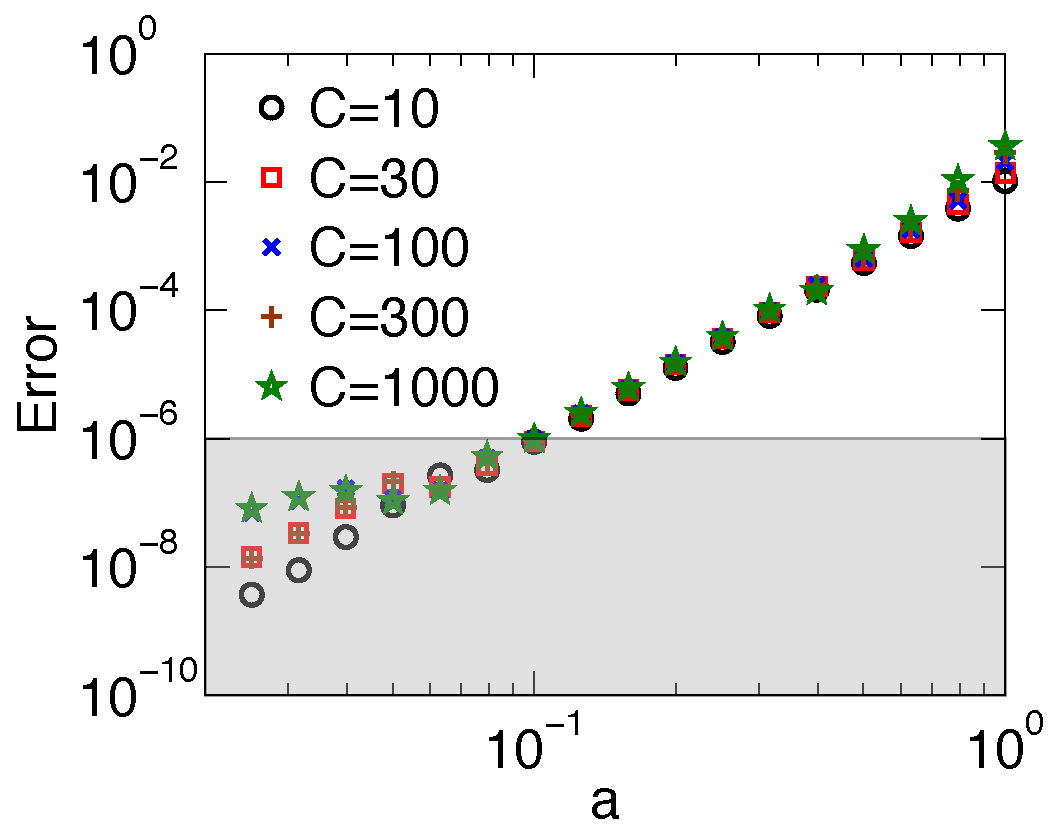
\includegraphics[width=0.5\textwidth]{./figs_Borregaard_PRL2015/figureSN3} 
\caption
[Conditional fidelity]
{ 
\label{fig:F}
Conditional infidelity of the gate as a function of the driving strength $(a)$
for $\gamma/\kappa = 0.01$, $\gamma_g = 0$, and $C\in\{10,30,100,300,1000\}$.
The shaded region (at $\sim 10^{-6}$) shows the limit of numerical accuracy. The
driving strength was assumed to be $\Omega=a\gamma\sqrt{C}$.}
\end{figure} 

We repeated the above analysis for the two-photon-driving Hamiltonian in
Eq.~\eqref{eq:supphamil2}. We chose $ \gamma = \gamma_g = \gamma_f =
0.01\,\kappa$,  $\Omega = \frac{\Delta_{E2}}{8 C^{1/4}}$, and
$\Omega_{\text{MW}} = 4\gamma C^{1/4}$, and chose $\Delta_E$ and $\Delta_e$
detunings again close to their adiabatic optimum, but numerically optimized them
with the same procedure as previously.
Plots of Fig.\ref{fig:t,P 2} show the gate time and the success probability as a
function of $\Delta_{E2}$ for $C\in\{10, 20, 50,100\}$. Symbols indicate the
numerical results while solid lines show the theoretical values.
 \begin{figure}[h]
\centering
\includegraphics[width=0.48\textwidth]{./figs_Borregaard_PRL2015/figureSN4}\quad 
\includegraphics[width=0.48\textwidth]{./figs_Borregaard_PRL2015/figureSN5}
\caption
[Gate time and success probability vs detuning]
{
\label{fig:t,P 2} 
Gate time (left) and failure probability (right) as a function of $\Delta_{E2}$
for $\gamma = \gamma_g = \gamma_f = 0.01\kappa$, $\Omega = \frac{\Delta_{E2}}{8
C^{1/4}}$, $\Omega_{\text{MW}} = 4\gamma C^{1/4}$, $C = \{10,20,50,100\}$.
	}
\end{figure} 
Fig.~2b in the article shows the conditional \emph{in}fidelity of the
two-photon-driven gate as a function of $C$ for the same choice of parameters.
With these results, we confirm that by increasing $\Delta_{E2}$ we can lower the
infidelity error to an arbitrary small level. The gate time is a constant of the
cooperativity since we have increased $\Omega_{MW}$ as $C^{1/4}$ in the
simulations. We do see some deviation from the analytical results due to
non-adiabatic effects, which could be suppressed by decreasing $\Omega$ at the
expense of an increase in the gate time. Finally a gradual ramping of $\Omega$
could also decrease the non-adiabatic errors but for simplicity, we have not
included this in the simulations.

\section{Additional errors} 

There are some additional errors in a realistic atomic setup that we have not
treated in detail so far. Here we estimate the dominant errors and determine
under which conditions, they can be sufficiently suppressed such that they do
not limit the performance of the gates. We assume a realistic atomic setup where
${}^{87}$Rb atoms are used both for the auxiliary atom and the qubit atoms. In
the ${}^{87}$Rb atoms, we assume that $\ket{g}=\ket{1,1}, \ket{f}=\ket{2,2}$ and
$\ket{E_{2}}=\ket{2^{e},2^{e}}, \ket{E}=\ket{3^{e},3^{e}}$ where
$\ket{r^{(e)},r^{(e)}}$ with $r=1,2,3$ refers to state
$\ket{\text{F}^{(e)}=r,\text{m}_{\text{F}}^{(e)}=r}$ in $5^{2}S_{1/2}$
$(5^{2}P_{3/2})$. In this case, we estimate that the dominant errors are:
\begin{itemize}
\item In our perturbative theory, we have assumed that the laser field ($\Omega$) only couple $\ket{g}\to\ket{E2}$ in the auxiliary atom. However, for a large detuning $\Delta_{E2}$ it may also couple $\ket{f}\to\ket{E}$, which could lead to an undetectable error where the auxiliary atom is pumped back to $\ket{E2}$ from, which it decays to $\ket{g}$. This error is, however, suppressed by the large frequency separation, $\Delta_{g}$ of $\ket{g}$ and $\ket{f}$, which is $\Delta_{g}\sim1000\gamma$ for ${}^{87}$ Rb. We estimate the error using effective operators to find the decay rate back to $\ket{g}$, assuming that the auxiliary atom starts in $\ket{E2}$ and treating the drive $\Omega$ as a perturbation while neglecting the cavity coupling. This is valid as long as $\Delta_{g}\gg\Delta_{E}$, which is fulfilled for $C\lesssim10000$ since $\Delta_{E}\sim\sqrt{C}$. The error increases with $\Delta_{E2}$ but even for $\Delta_{E2}\approx400\gamma$ we find that for $\Omega_{\text{MW}}=4\gamma C^{1/4}$, $\Omega=\Delta_{E2}/8$ the error is $\lesssim10^{-4}$.     

\item The microwave might also couple the ground states $\ket{0}-\ket{1}$ of the
qubit atoms and the ground states $\ket{g}-\ket{f}$ of the auxiliary atom. The
coupling of $\ket{0}-\ket{1}$ means that the qubit atoms also couple to the
cavity even though they are in state $\ket{0}$. We estimate the error from this
to be on the order of
$\Omega_{\text{MW}}^{2}/(\Delta_{g}-(\Delta_{E2}-\Delta_{E}+\Delta_{2\to3}))^2$
where $\Delta_{2\to3}$ is the splitting between $\ket{E_{2}}$ and $\ket{E}$. For
${}^{87}$Rb, $\Delta_{2\to3}\approx44\gamma$. Below we argue that we need
$\Delta_{E}<0$. Since $\Delta_{E}\approx-\sqrt{C}\gamma$ this error will
increase slowly with cooperativity but it is suppressed by $\Delta_{g}$. For
$\Omega_{\text{MW}}=4\gamma C^{1/4}$, we find that the error is
$\lesssim10^{-4}$ for $C\lesssim1000$ even for $\Delta_{E2}\approx400\gamma$.
The errors from the coupling of the states $\ket{g}-\ket{f}$ in the auxiliary
atom will likewise be suppressed by the large energy splitting $\Delta_{g}$.
These errors can also be further suppressed by decreasing $\Omega_{\text{MW}}$
at the cost of a larger gate time.
\end{itemize}

The above errors can be highly suppressed using e.g.${}^{88}$Sr,
${}^{138}$Ba${}^{+}$ or ${}^{40}$Ca${}^{+}$ instead of ${}^{87}$Rb. For these
atoms, the ground states can be encoded in the $S_{0}$ and $P_{0}$ manifoldes
for ${}^{88}$Sr and the $S_{1/2}$ and $D_{3/5}$ manifolds for
${}^{138}$Ba${}^{+}$ and ${}^{40}$Ca${}^{+}$, which have separations at optical
frequencies between the stable states.

A final error that we will consider is that the transition
$\ket{E}\leftrightarrow\ket{f}$ will not be completely closed if the cavity is
linearly polarized. This will, e.g. be the case for the system in Ref.
\cite{thompson}. Such a cavity also couples $\ket{f}$ to the states
$\ket{1^{e},1^{e}},\ket{2^{e},1^{e}}$ and $\ket{3^{e},1^{e}}$. From
$\ket{1^{e},1^{e}}$ and $\ket{2^{e},1^{e}}$ there might be an undetectable decay
back to $\ket{g}$, which will introduce an error $\propto1/\sqrt{C}$ in the
gates. The probability of an undetectable decay from these states should be
compared to the probability of the detectable decays where the cavity photon is
scattered of the qubit atoms instead. For ${}^{87}$Rb, we estimate this error by
compairing the strengths of the effective couplings from $\ket{f}$ to
$\ket{1^{e},1^{e}}$ and $\ket{2^{e},1^{e}}$ with a subsequent decay to $\ket{g}$
with the strength of the effective coupling from $\ket{1}$ to $\ket{e}$ in the
qubit atoms with a subsequent decay back to $\ket{1}$. The latter process has a
detuning of $\Delta_{E}$ while the first two are additional detuned by the
energy gaps between $\ket{3^{e},3^{e}}$ and $\ket{1^{e},1^{e}}$ and
$\ket{3^{e},3^{e}}$ and $\ket{2^{e},1^{e}}$ respectively, assuming that
$\Delta_{E}<0$. We find that since $\abs{\Delta_{E}}$ grows as $\sqrt{C}$ the
error increases from $\sim5\cdot10^{-5}$ at $C=1$  to a maximum value of
$\sim2\cdot10^{-3}$ for $C\sim3000$ for which $\Delta_{E}$ is comparable to the
extra detunings of the $\ket{1^{e},1^{e}}$ and $\ket{2^{e},1^{e}}$ transitions
compared to the $\ket{e}$ transition. For $C>3000$ the error decreases as
$1/\sqrt{C}$.
Note that this error could be removed  by making a 4 photon drive from $\ket{g}$
to $\ket{E}$ by letting $\ket{g}=\ket{1,-1}$. Another approach is to consider
other atoms such as ${}^{40}$Ca${}^{+}$, with more favorable levelstructures.
The state $\ket{g}$ could be encoded in the $3^{2}D_{5/2}$ subspace while the
state $\ket{f}$ could be encoded in the $4^{2}S_{1/2}$ subspace and similarly
for the qubit states $\ket{0}$ and $\ket{1}$. In such a setup, we will have
separations of optical frequencies between the qubit states and we can remove
the decay from the excited state back to $\ket{g}$ by, e.g. driving from
$3^{2}D_{5/2}$ to $4^{2}P_{1/2}$ through $3^{2}D_{3/2}$.

\chapter{Appendices for Chapter \ref{ch:Borregaard_PRA2015}}
\label{app:Borregaard_PRA2015}

\section{Error analysis of the single-photon scheme} \label{single}

The setup of the single-photon scheme is described in Sec. \ref{sec:1phot}. The
single photon detectors are assumed to have a dark count probability of
$P_{\text{dark}}$ and an efficiency of $\eta_{\text{d}}$ while the transmission
efficiency of the fibers is denoted $\eta_{\text{f}}$.  As described in Sec.
\ref{sec:generation}, the probability of an emitter to go from the excited
state, $\ket{e}$ to the ground state $\ket{1}$ is $P_{\text{phot}}$ while the
excitation probability is $\epsilon^{2}$. The scheme is conditioned on a single
click at the central station. Depending on which detector gave the click, a
single qubit rotation can be employed such that ideally the state
$\ket{\Psi^{+}}$ is created. Going through all the possibilities of obtaining a
single click at the central station, we find that the density matrix following a
single click, and possible subsequent single qubit rotations, is
\begin{eqnarray}
\rho_{1click}&=&F_{1}\ket{\Psi^{+}}\bra{\Psi^{+}}+
\alpha_{1}\ket{\Phi^{+}}\bra{\Phi^{+}}+\alpha_{1}
\ket{\Phi^{-}}\bra{\Phi^{-}}\qquad\nonumber
\\
&&+\beta_{1}\ket{\Psi^{-}}\bra{\Psi^{-}}+
\tilde{\alpha}_{1}\ket{00}\bra{00}+ \tilde{\beta}_{1}\ket{11}\bra{11},
\end{eqnarray}
with coefficients
\begin{eqnarray}
&&F_{1}=\frac{1}{P_{\text{1click}}}
\Big[2\eta_{\text{d}}\eta_{\text{f}}P_p
\epsilon^{2}(1-\epsilon^{2})(1-P_d)
+2\eta_{\text{f}}(1-\eta_{\text{d}})P_p
\epsilon^{2}(1-\epsilon^{2})P_d(1-P_d)\nonumber
\\
&&\qquad+\frac{1}{2}\eta_{\text{d}}\eta_{\text{f}}P_p
\epsilon^{4}(1-P_p(1-P_d)+2(1-\eta_{\text{f}})P_p\epsilon^{2}(1-
\epsilon^{2})P_d(1-P_d) \nonumber \\
&&\qquad+(1-\eta_{\text{d}}\eta_{\text{f}})P_p
\epsilon^{4}(1-P_p)P_d(1-P_d)+(1-\epsilon^{2})\epsilon^{2}(1-P_p)
P_d(1-P_d)\nonumber
\\
&&\qquad+\frac{1}{2}\epsilon^{2}(1-P_p)^{2}
P_d(1-P_d)\Big] 
\\
&&\alpha_{1}=\frac{1}{P_{\text{1click}}}\Big[\frac{1}{2}
\epsilon^{2}(1-P_p)^{2}P_d (1-P_d)\Big]
\\
&&\beta_{1}=\frac{1}{P_{\text{1click}}}\Big[\frac{1}{2}\eta_{\text{d}}
\eta_{\text{f}}P_p\epsilon^{4}(1-P_p)
(1-P_d) +2(1-\eta_{\text{f}})P_p\epsilon^{2}
(1-\epsilon^{2})P_d(1-P_d) \nonumber \\
&&\qquad+(1-\eta_{\text{d}}\eta_{\text{f}})P_p
\epsilon^{4}(1-P_p)P_d(1-P_d)
+(1-\epsilon^{2})\epsilon^{2}(1-P_p)
P_d(1-P_d) \nonumber \\
&&\qquad+\frac{1}{2}\epsilon^{2}(1-P_p)^{2}
P_d(1-P_d) 
+2\eta_{\text{f}}(1-\eta_{\text{d}})P_p
\epsilon^{2}(1-\epsilon^{2})P_d(1-P_d)\Big] 
\\
&&\tilde{\alpha}_{1}=\frac{1}{P_{\text{1click}}}
\Big[2(1-\epsilon^{2})^{2}P_d(1-P_d)
+2(1-\epsilon^{2})\epsilon^{2}(1-P_p)
P_d(1-P_d)\Big] 
\\
&&\tilde{\beta}_{1}=\frac{1}{P_{\text{1click}}}
\Big[\eta_{\text{d}}\eta_{\text{f}}P_p
\epsilon^{4}(1-P_p)(1-P_d)
+2(1-\eta_{\text{d}}\eta_{\text{f}})P_p
\epsilon^{4}(1-P_p)P_d(1-P_d) \nonumber \\
&&\qquad +2(1-\eta_{\text{d}}\eta_{\text{f}})^{2}
P_p^{2}\epsilon^{4}P_d(1-P_d)
+2(1-\eta_{\text{d}}\eta_{\text{f}})
\eta_{\text{d}}\eta_{\text{f}}P_p^{2}
\epsilon^{4}(1-P_d)^{2}\Big],
\end{eqnarray}
where $P_d = P_{\text{dark}}$ and $P_p = P_{\text{phot}}$.
Here we have assumed that with probability $\epsilon^{2}(1-P_{\text{phot}})$, an
emitter is excited but spontaneously decay to the ground states instead of
emitting a cavity photon. Furthermore, we have assumed that the decay rates to
the two ground states are equal such that the emitter ends up in
$\frac{1}{2}(\ket{0}\bra{0}+\ket{1}\bra{1})$. Note that the detectors are not
assumed to be number resolving.  $P_{\text{1click}}$ is the total success
probability given by
\begin{eqnarray}
P_{\text{1click}}&=&2\eta_{\text{d}}
\eta_{\text{f}}P_{\text{phot}}\epsilon^{2}
(1-P_{\text{phot}}\epsilon^{2})(1-P_{\text{dark}})
+(2\eta_{\text{f}}\eta_{\text{d}}-
\eta_{\text{f}}^{2}\eta_{\text{d}}^{2}) P_{\text{phot}}^{2}\epsilon^{4}
\nonumber \\
&&+2(1-\epsilon^{2}P_{\text{phot}})^{2}
P_{\text{dark}}(1-P_{\text{dark}}) +2(1-\eta_{\text{d}}\eta_{\text{f}})^{2}
P_{\text{phot}}^{2}\epsilon^{4}P_{\text{dark}}(1-P_{\text{dark}})\nonumber \\
&&+4(1\!-\!\eta_{\text{d}}\eta_{\text{f}}) P_{\text{phot}}\epsilon^{2}
(1\!-\!\epsilon^{2}P_{\text{phot}}) P_{\text{dark}}(1\!-\!P_{\text{dark}}).
\end{eqnarray}
Assuming $P_{\text{dark}}\ll1$, the dominant error is where both qubits are
excited but only a single click is detected at the central station. This leaves
the qubits in the state $\ket{11}\bra{11}$ and this error is efficiently
detected by the purification scheme described in Ref. \cite{bennett}.

\section{Error analysis of the two-photon scheme} \label{two}

For the two photon scheme described in Sec. \ref{sec:generation}, we condition
on a click in two detectors. Once again we assume that appropriate single qubit
rotations are employed depending on which detector combination clicked such that
ideally the state $\ket{\Phi^{+}}$ is created. We find that the density matrix
describing the qubit state after a successful event is
\begin{eqnarray}
\rho_{2click}&=&F_{2}\ket{\Phi^{+}}\bra{\Phi^{+}}+\alpha_{2}\ket{\Psi^{+}}
\bra{\Psi^{+}}+\alpha_{2}\ket{\Psi^{-}}\bra{\Psi^{-}}+\beta_{2}\ket{\Phi^{-}}\bra{\Phi^{-}},
\end{eqnarray} 
where we have defined
\begin{eqnarray}
F_{2}&=&\frac{(1-P_{\text{dark}})^{2}}{P_{\text{2click}}}
\Big[\frac{1}{2}\eta_{d}^{2}\eta_{\text{f}}^{2}P_{\text{phot}}^{2} 
+\eta_{\text{d}}(1-\eta_{\text{d}})\eta_{\text{f}}^{2}
P_{\text{dark}}P_{\text{phot}}^{2}
+\eta_{\text{f}}^{2}(1-\eta_{\text{d}})^{2}P_{\text{phot}}^{2}
P_{\text{dark}}^{2}\nonumber \\
&&+P_{\text{dark}}^{2}(1-P_{\text{phot}})^{2}+\eta_{\text{d}}
(1-\eta_{\text{f}})\eta_{\text{f}}P_{\text{dark}}P_{\text{phot}}^{2}
+\eta_{\text{d}}\eta_{\text{f}}P_{\text{dark}}P_{\text{phot}}
(1-P_{\text{phot}})\nonumber \\
&&+(1-\eta_{\text{f}})^{2}P_{\text{phot}}^{2}P_{\text{dark}}^{2}
 +2\eta_{\text{f}}(1-\eta_{\text{d}})(1-\eta_{\text{f}})
P_{\text{phot}}^{2}P_{\text{dark}}^{2}\nonumber \\
&&+2(1-\eta_{\text{d}}\eta_{\text{f}})P_{\text{phot}}
(1-P_{\text{phot}})P_{\text{dark}}^{2}\Big]  
\\
\alpha_{2}&=&\frac{(1-P_{\text{dark}})^{2}}{P_{\text{2click}}}
\Big[\eta_{d}(1-\eta_{\text{f}})\eta_{\text{f}}P_{\text{dark}}
P_{\text{phot}}^{2} +P_{\text{dark}}^{2}(1-P_{\text{phot}})^{2}+\nonumber \\
&&\eta_{\text{d}}
\eta_{\text{f}}P_{\text{dark}}P_{\text{phot}}(1-P_{\text{phot}})
+(1-\eta_{\text{f}})^{2}P_{\text{phot}}^{2}P_{\text{dark}}^{2}\nonumber \\
&&+2\eta_{\text{f}}(1-\eta_{\text{d}})(1-\eta_{\text{f}})
P_{\text{phot}}^{2}P_{\text{dark}}^{2}
 +2(1-\eta_{\text{d}}\eta_{\text{f}})P_{\text{phot}}
(1-P_{\text{phot}})P_{\text{dark}}^{2}\nonumber \\
&&+\eta_{\text{d}}(1-\eta_{\text{d}})\eta_{\text{f}}^{2}
P_{\text{dark}}P_{\text{phot}}^{2}
 +\eta_{\text{f}}^{2}(1-\eta_{\text{d}})^{2}P_{\text{phot}}^{2}
P_{\text{dark}}^{2}\Big]  
\\
\beta_{2}&=&\alpha_{2}+\frac{(1-P_{\text{dark}})^{2}}
{P_{\text{2click}}}\Big[\eta_{\text{d}}(1-\eta_{\text{d}})
\eta_{\text{f}}^{2}P_{\text{dark}}P_{\text{phot}}^{2}
+\eta_{\text{f}}^{2}(1-\eta_{\text{d}})^{2}P_{\text{phot}}^{2}
P_{\text{dark}}^{2}\Big].
\end{eqnarray}
The success probability $P_{\text{2click}}$ is 
\begin{eqnarray}
P_{\text{2click}}&=&(1-P_{\text{dark}})^{2}\Big[\frac{1}{2}
\eta_{\text{d}}^{2}\eta_{\text{f}}^{2}P_{\text{phot}}^{2} 
 +4\eta_{\text{d}}\eta_{\text{f}}(1-\eta_{\text{d}}\eta_{\text{f}})
P_{\text{dark}}P_{\text{phot}}^{2}
+4P_{\text{dark}}^{2}(1-P_{\text{dark}})^{2} \nonumber \\
&&+4\eta_{\text{d}}\eta_{\text{f}}P_{\text{dark}}P_{\text{phot}}
(1-P_{\text{phot}})+4(1-\eta_{\text{d}}\eta_{\text{f}})^{2}P_{\text{phot}}^{2}
P_{\text{dark}}^{2} 
\nonumber \\
&&+8(1-\eta_{\text{d}}\eta_{\text{f}})P_{\text{phot}}
(1-P_{\text{phot}})P_{\text{dark}}^{2}\Big]
\end{eqnarray}
As in the single-photon scheme, we have not assumed number resolving detectors
and we have assumed that with probability ($1-P_{\text{phot}}$), an emitter
spontaneously decay to one of the ground states resulting in the state
$\frac{1}{2}(\ket{0}\bra{0}+\ket{1}\bra{1})$.

\section{Deterministic CNOT gate} \label{app:cnot}

Here we describe the local entanglement generation scheme presented in
Ref.~\cite{Anders1prl}, which can be used to make a deterministic CNOT gate as
described in Section \ref{sec:CNOTgate}. We assume that weak coherent light
is continuously shined onto the cavity such that at most one photon is in the
cavity at all times. A single-photon detector continuously monitors if any
photons are reflected from the cavity and the coherent light is blocked if a
click is recorded before $n_{max}$ photons on average have been sent onto the
cavity. If no click was recorded during this time, both atoms are interpreted as
being in the $g$ levels. The steps of the entangling scheme are the following.
\begin{enumerate}
\item  Both atoms are initially prepared in the superposition $\ket{g}+\ket{f}$
by e.g. a $\pi/2$-pulse.
\item Coherent light is sent onto the cavity.  If a click is recorded before on
average $n_{\text{max}}$ photons have been sent onto the cavity, the levels of
the atoms are flipped ($\ket{g}\leftrightarrow\ket{f}$). If no click is
recorded, the atoms are interpreted as being in $\ket{gg}$ and the procedure is
repeated from step 1.
\item Conditioned on the first click, another coherent light pulse is sent onto
the cavity after the levels of the atoms have been flipped. If a click is
recorded before $n=n_{\text{max}}-n_{1}$ photons on average have been sent onto
the cavity, the entangling scheme is considered to be a success. Here $n_{1}$ is
the average number of photons that had been sent onto the cavity before the
first click. If no click is recorded, the atoms are interpreted as being in
$\ket{gg}$ and the procedure is repeated from step 1.
\end{enumerate}
As described above, the entangling scheme is repeated until it is successful leading to a deterministic creation of entanglement in the end. As described in Ref. \cite{Anders2prl} a series of non-destructive measurements of the atoms together with single qubit rotations can be used to make a CNOT operation after the entanglement has been created. The non-destructive measurements can be performed using the same technique of monitoring reflected light as in the entangling scheme and we assume that we can effectively tune the couplings to the cavity such that possibly only a single atom couples.

\section{Rate analysis} \label{app:rate}

Here we analyse the rate of entanglement distribution for the different repeater
architectures considered in the main text. The total rate of the repeater is set
by the average time of entanglement creation, initial purification and
entanglement swapping. Assuming that entanglement generation has a success
probability, $P_{0}$, we estimate the average time $\tau_{\text{pair},l;m}$ it
takes to generate $l$ entangled pairs in one elementary link using $m$ qubits,
which can be operated in parallel, as
\begin{equation}
\tau_{\text{pair},l;m}=\mathcal{Z}_{l;m}(P_{0})(L_{0}/c+\tau_{\text{local}}).
\end{equation}
Here $c$ is the speed of light in the fibers and $\tau_{\text{local}}$ is the
time of local operations such as initialization of the qubits. The factor
$\mathcal{Z}_{l;m}(P_{0})$ can be thought of as the average number of coin
tosses needed to get at least $l$ tails if we have access to $m$ coins, which we
can flip simultaneously and the probability of tail is $P_{0}$ for each coin
\cite{bernardes}. It is furthermore assumed that coins showing tail after a toss
are kept and only the coins showing head are tossed again until $l$ tails are
obtained. In the repeater context, the coins are entanglement generation
attempts and tail is successful entanglement generation. The time it takes per
"toss" is $L_{0}/c+\tau_{\text{local}}$. To calculate the expressions for
$Z_{l;m}(P_{0})$, we follow the lines of Ref. \cite{bernardes} where similar
factors are derived. The expression for $\mathcal{Z}_{m;m}(p)$ is already
derived in Ref. \cite{bernardes} and their result is stated below
\begin{equation}
\mathcal{Z}_{m;m}=\sum_{k=1}^{m}\binom{m}{k}\frac{(-1)^{k+1}}{1-(1-p)^{k}}. 
\end{equation}
For $\mathcal{Z}_{l;m}$ where $l\neq m$, we only need to find expressions for
$\mathcal{Z}_{1;m}$ with $m=1,2,3,4$, $\mathcal{Z}_{2;m}$ with $m=3,4$ and
$\mathcal{Z}_{3;4}$ since we have a maximum of 4 qubits pr. repeater station.
For $\mathcal{Z}_{2;3}$, we have that
\begin{eqnarray} \label{eq:suppf}
\mathcal{Z}_{2:3}&=&\binom{3}{3}\sum_{k=1}^{\infty}
k(q^{3})^{k-1}p^{3}+\binom{3}{2}\sum_{k=1}^{\infty} k(q^{3})^{k-1}p^{2}q \qquad
\nonumber \\
&&+\binom{3}{1}\binom{2}{1}\sum_{k=1}^{\infty}
\sum_{l=1}^{\infty}(k+l)[(q^{3})^{k-1}pq^{2}][(q^{2})^{l-1}pq] \nonumber \\
&&+\binom{3}{1}\binom{2}{2}\sum_{k=1}^{\infty}
\sum_{l=1}^{\infty}(k+l)[(q^{3})^{k-1}pq^{2}][(q^{2})^{l-1}p^{2}],
\end{eqnarray}
where $q=1-p$. 
The first term in Eq.~\eqref{eq:suppf} describes the situations where three
tails are obtained in a single toss after a given number of tosses, where all
coins showed head.  We will refer tosses where all coins show tail as failed
tosses. The second term describes the situation where we get two tails in the
same toss after a given number of failed tosses. The third and fourth terms are
where we get a single tail after a given number of failed tosses. The coin
showing tail is then kept and the two remaining coins are tossed until we obtain
another tail (third term) or two tails simultaneously (fourth term). The
geometric series in Eq.~\eqref{eq:suppf} can be solved to give
\begin{equation}
\mathcal{Z}_{2;3}=\frac{5-(7-3p)}{(2-p)p(3+(p-3)p)} \approx\frac{5}{6p},
\end{equation} 
where the approximate expression is for $p\ll1$. Note that the factor of
$\frac{5}{6}$ corresponds to a simple picture where it on average takes
$\frac{1}{3}\frac{1}{p}$ attempts to get the first 'tail' using 3 coins and
$\frac{1}{2}\frac{1}{p}$ attempts to get the second using the remaining $2$
coins. In a similar manner, we find that
\begin{eqnarray}
\mathcal{Z}_{1;2}&=&\frac{1}{2p-p^{2}}\approx\frac{1}{2p} \\
\mathcal{Z}_{1;3}&=&\frac{1}{3p-3p^{2}+p^{3}}\approx\frac{1}{3p} \\
\mathcal{Z}_{1;4}&=&\frac{1}{4p-6p^{2}+4p^{3}-p^{4}}\approx\frac{1}{4p} \\
\mathcal{Z}_{2;4}&=&\frac{-7+p(15+p(4p-13))}{(p-2)p(3+(p-3)p)(2+(p-2)p)}
\approx\frac{7}{12p} \\
\mathcal{Z}_{3;4}&=&\frac{-13+p(33+p(22p-6p^{2}-37))}
{(p-2)p(3+(p-3)p)(2+(p-2)p)}
\approx\frac{13}{12p}. 
\end{eqnarray}
Here the approximate expressions are all for $p\ll1$ and they correspond to the
expressions one would get using simple pictures similar to the one described
above in the discussion of $\mathcal{Z}_{2;3}$.

After creating a number of entangled pairs in an elementary link of the
repeater, they may be combined to create a purified pair of higher fidelity. As
previously mentioned, we assume an entanglement pumping scheme since this
requires less qubit resources than a cascading scheme. Let
$P_{\text{pur}}(F_{0},F_{0})$ denote the success probability of the purification
operation, which depends on the fidelity of the two initial pairs ($F_{0}$) and
the fidelity of the CNOT gate used in the purification operation. Note that
$P_{\text{pur}}$ also contains the success probability of the CNOT gate used in
the purification for the heralded gate. We estimate the average time
$\tau_{\text{pur},1}$, it takes to make one purified pair from two initial pairs
of fidelity $F_{0}$, using $m$ qubits in parallel in the entanglement generation
step, as
\begin{equation}
\tau_{\text{pur},1}=\frac{\tau_{\text{pair},2;m}+\tau_{\text{pur}}}
{P_{\text{pur}}(F_{0},F_{0})},
\end{equation}     
where $\tau_{\text{pur}}\sim L_{0}/c+\tau_{\text{c}}$ is the time of the
purification operation including the classical comunication time required to
compare results. Here $\tau_{\text{c}}$ is the time of the CNOT operation and
$L_{0}/c$  is the communication time between the two repeater stations sharing
the entangled pairs. To further pump the entanglement of the purified pair, a
new entangled pair is subsequently created using $m-1$ qubits operated in
parallel. The average time it takes to make $j$ rounds of purification is thus
estimated as
\begin{equation} \label{eq:pur1}
\tau_{\text{pur},j}=\frac{\tau_{\text{pur},j-1}+
\tau_{pur}+\tau_{\text{pair},1:m-1}}{P_{\text{pur}}(F_{j-1},F_{0})},
\end{equation}
with $\tau_{\text{pur},0}=\tau_{\text{pair},2;m}- \tau_{\text{pair},1:m-1}$.
Here $F_{j-1}$ is the fidelity of the purified pair after $j-1$ purifications.
The total rate of a repeater, consisting both of purification and entanglement
swapping, depends on the specific repeater achitecture. We will first consider
the case of both a parallel and sequential repeater operated with deterministic
gates and afterwards the same situations with probabilistic gates.

\subsection{Deterministic gates}

For a parallel repeater with $n$ swap levels and deterministic gates, we first
estimate the average time it takes to generate $2^{n}$ purified pairs, i.e. a
purified pair in each elementary link. We assume that each pair is purified $j$
times such that the time to generate one purified pair is
\begin{eqnarray} \label{eq:pur2}
\tau_{\text{pur},j}&=&\frac{\mathcal{Z}_{2;m}(P_{0})
(L_{0}/c+\tau_{\text{local}})}{P_{\text{pur}}(F_{0},F_{0}) \cdots
P_{\text{pur}}(F_{j-1},F_{0})}+\sum_{i=0}^{j-1}\frac{\tau_{\text{pur}}}{P_{\text{pur}} (F_{i},F_{0})\cdots
P_{\text{pur}}(F_{j-1},F_{0})} 
\nonumber \\
&&+\sum_{i=1}^{j-1}\frac{\mathcal{Z}_{1;m-1}(P_{0})(L_{0}/c+ \tau_{\text{local}})}{P_{\text{pur}}(F_{i},F_{0})\cdots 
P_{\text{pur}}(F_{j-1},F_{0})},
\end{eqnarray}
where we have solved the recurrence in Eq.~\eqref{eq:pur1}. We now wish to
estimate the total time, $\tau_{\text{link},2^{n}}$ it takes to make
purification in every elementary link, i.e. the time it takes to make $2^{n}$
pairs. A lower limit of $\tau_{\text{link},2^{n}}$ is simply
$\tau_{\text{pur},j}$ but this is a very crude estimate if the purification have
a limited success probability since the time is not determined by the average
time but by the average time for the last link to succeed. We therefore make
another estimate of the average time by treating $\tau_{\text{pur},j}$ as
consisting of $2j$ independent binomial events with probabilities
\begin{eqnarray}
P_{1}&=&\frac{P_{\text{pur}}(F_{0},F_{0})\cdots P_{\text{pur}}
(F_{j-1},F_{0})}{\mathcal{Z}_{2;m}(P_{0})} \\
P_{2}^{(i)}&=&P_{\text{pur}}(F_{i},F_{0})\cdots P_{\text{pur}} (F_{j-1},F_{0})
\\
P_{3}^{(i)}&=&\frac{P_{\text{pur}}(F_{i},F_{0})\cdots P_{\text{pur}}
(F_{j-1},F_{0})}{\mathcal{Z}_{1;m-1}(P_{0})}.
\end{eqnarray}
We then estimate the average time, $\tau_{link,2^{n}}$ it takes to make $2^{n}$
purified pairs as
\begin{eqnarray} \label{eq:purnlink}
\tau_{\text{link},2^{n}}&=&\mathcal{Z}_{2^{n};2^{n}}(P_{1})
(L_{0}/c+\tau_{\text{local}}) 
 +\sum_{i=0}^{j-1}\mathcal{Z}_{2^{n},2^{n}}(P_{2}^{(i)}) \tau_{\text{pur}}
\nonumber \\
&&+\sum_{i=1}^{j-1}\mathcal{Z}_{2^{n},2^{n}}(P_{3}^{(i)})
(L_{0}/c+\tau_{\text{local}}).
\end{eqnarray}
Eq.~\eqref{eq:purnlink} is a better estimate for the average time than
$\tau_{\text{pur},j}$ in the limit of small success probabilities since it takes
into account that we need success in all links. This is contained in the factors
$\mathcal{Z}_{2^{n};2^{n}}$. However, it overestimates the average distribution
time when the purification has a large success probability. How much it
overestimates depends on $n$ and $j$. Comparing  $\tau_{\text{pur},j}$ to
Eq.~\eqref{eq:purnlink} we find numerically that for $n\leq5$ and $j\leq2$ there
is a factor $\lesssim2$ between the two estimates, in the limit of large success
probability for the purification operation. As discussed in Sec.~\ref{sec:optim}
we never consider more than 5 swap levels in our optimization and since we have
a limited number of qubits pr. repeater station, we will never have to consider
more than 2 rounds of purification. We can therefore use the estimate for
$\tau_{\text{link},2^{n}}$ given in Eq.~\eqref{eq:purnlink}.

To get the average time it takes to distribute one entangled pair over the total
distance, $L_{tot}$, of the repeater, we need to add the time of the
entanglement swapping, $\tau_{\text{swap},nd}$ to $\tau_{\text{link},2^{n}}$. We
estimate $\tau_{\text{swap},n}$ as
\begin{equation}
\tau_{\text{swap},n}=(2^{n}-1)L_{0}/c+n\tau_{\text{c}},
\end{equation} 
where the first term is the time of the classical communication and
$\tau_{\text{c}}$ is the time of the CNOT operation involved in the swap
procedure. The average distribution rate, of a parallel repeater with
deterministic gates, is thus
$r=1/(\tau_{\text{link},2^{n}}+/\tau_{\text{swap},n})$.

For a repeater using sequential entanglement creation with deterministic gates,
we estimate the time it takes to generate purified pairs in all $2^{n}$ pairs as
\begin{equation}
\tau^{(s)}_{\text{link},2^{n}}=\left(\tau_{\text{link},2^{n-1}}\right)\vline_{m\to2m}+\left(\tau_{\text{link},2^{n-1}}\right)\vline_{m\to2m-1}.
\end{equation}
Here we have indicated that the number of qubits, which can be operated in
parallel is $2m$ for the first $2^{n-1}$ pairs and $2m-1$ for the next $2^{n-1}$
pair compared to the parallel repeater, where only $m$ qubits can be used in all
$2^{n}$ pairs. Note, that we have assumed that first entanglement is established
in half of the links and only when this is completed, entanglement is created in
the remaining half of the links. This is clearly not the fastest way of
operating the repeater but it gives an upper limit of the average distribution
time and hence a lower limit on the rate. The entanglement swapping of the
sequential repeater is exactly the same as for the parallel repeater and the
average total rate, of the sequential repeater with deterministic gates, is thus
$r=1/(\tau^{(s)}_{\text{link},2^{n}}+t_{\text{swap},n})$.

\subsection{Probabilistic gates}

To estimate the total, average distribution time of a repeater using parallel
entanglement creation with $n$ swap levels and probabilistic gates, we will
again treat $\tau_{\text{pur},j}$ as consisting of $2j$ independent binomial
events, as we did for the deterministic gates. The time it takes to make a
single swap can be estimated as
\begin{eqnarray} \label{eq:swap1}
\tau_{\text{swap},1}&=&\frac{\mathcal{Z}_{2;2}
(P_{1})(L_{0}/c+\tau_{\text{local}})}{P_{\text{swap}}}+
\frac{L_{0}/c}{P_{\text{swap}}}+\frac{\tau_{\text{c}}}{P_{\text{swap}}} \nonumber \\
&&+\sum_{i=0}^{j-1}\frac{\mathcal{Z}_{2;2}
(P_{2}^{(i)})\tau_{\text{pur}}}{P_{\text{swap}}} +\sum_{i=1}^{j}\frac{\mathcal{Z}_{2;2}(P_{3}^{(i)})
(L_{0}/c+\tau_{\text{local}})}{P_{\text{swap}}},
\end{eqnarray}
where $P_{\text{swap}}$ is the probability of the swap operation, i.e. the
probability of the CNOT gate. Eq.~\eqref{eq:swap1} can be iterated such that the
average time it takes to make $n$ swap levels is estimated as
\begin{eqnarray} \label{eq:swap2}
\tau_{\text{swap},n}&=&\frac{\tilde{\mathcal{Z}}_{n;1}
(P_{\text{swap}},P_{1})(L_{0}/c+\tau_{\text{local}})}{P_{\text{swap}}} +\sum_{i=1}^{n}\frac{\tilde{\mathcal{Z}}_{n;i}
(P_{\text{swap}},P_{\text{swap}})(2^{i-1}L_{0}/c+\tau_{\text{c}})}
{P_{\text{swap}}} \nonumber \\
&&+\sum_{i=0}^{j-1}\frac{\tilde{\mathcal{Z}}_{n;1}
(P_{\text{swap}},P_{2}^{(i)})\tau_{\text{pur}}}{P_{\text{swap}}} +\sum_{i=1}^{j-1}\frac{\tilde{\mathcal{Z}}_{n;1}
(P_{\text{swap}},P_{3}^{(i)})(L_{0}/c+\tau_{\text{local}})}{P_{\text{swap}}}, \qquad
\end{eqnarray}
where 
\begin{eqnarray}
\tilde{\mathcal{Z}}_{n;i}(P_{\text{swap}},P)
&=&\mathcal{Z}_{2;2}\left(\frac{P_{\text{swap}}}
{\tilde{\mathcal{Z}}_{n-1;i}(P_{\text{swap}},P)}\right), \\ 
\tilde{\mathcal{Z}}_{i;i}(P_{\text{swap}},P)&=&\mathcal{Z}_{2;2}(P) \\
\tilde{\mathcal{Z}}_{i;i}(P_{\text{swap}},P_{\text{swap}})&=&1.
\end{eqnarray}
Here $P$ is either $P_{1}, P_{2}^{(i)}$ or $P_{3}^{(i)}$. In the limit of
$P_{0},P_{\text{swap}}\ll1$ and assuming no initial purification,
Eq.~\eqref{eq:swap2} reduces to the well-known fomula
\cite{sangouard3,sangouard2}
\begin{equation}
\tau_{\text{swap},n}=\frac{\left(3/2\right)^{n}
\left(L_{0}/c+\tau_{\text{local}}\right)}{P_{0}P_{swap}^{n}},
\end{equation}
since $\mathcal{Z}_{2;2}(P\ll1)\approx3/(2P)$ and the time of local operations
in the swaps can be neglected in this limit. However, for higher success
probabilities, Eq.~\eqref{eq:swap2} more accurately estimates the average
distribution time. The average rate of a parallel repeater with probabilistic
gates and $n$ swap levels is then $r=1/\tau_{\text{swap},n}$. From a numerical
study, we again find that for $P_{\text{swap}}\approx1$ and $P_{0}\ll1$,
Eq.~\eqref{eq:swap2} underestimates the average distribution rate with a factor
that increases with the number of swap levels, $n$. However, for $n\leq 5$ and
$j\leq2$, we find that this factor is $\lesssim2$.

The operation of a sequential repeater with probabilistic gates is not
straightforward since it is unclear how the sequential generation of
entanglement should take place after a failed swap operation. We therefore
choose to assume that initially, entanglement is generated in all $2^{n}$ links
sequentially. When this is completed the first round of entanglement swapping is
performed. If a swap fails, entanglement is restored in a parallel manner in
this section, i.e. the sequential operation is only employed in the initial
generation of entanglement. Thus if $i$'th swaps fail in the first swap level an
extra waiting time of
\begin{eqnarray} \label{eq:swap01}
&&\mathcal{Z}_{i;i}\left(\frac{P_{\text{swap}}}
{\mathcal{Z}_{2;2}(P_{1})}\right)(L_{0}/c+\tau_{\text{local}}) 
+\mathcal{Z}_{i;i}(P_{\text{swap}})(L_{0}/c+\tau_{\text{c}}) \nonumber \\
&&+\sum_{k=0}^{j-1}\mathcal{Z}_{i;i}
\left(\frac{P_{\text{swap}}}{\mathcal{Z}_{2;2}(P_{2}^{(k)})}
\right)\tau_{\text{pur}} 
+\sum_{k=1}^{j-1}\mathcal{Z}_{i;i}
\left(\frac{P_{\text{swap}}}{\mathcal{Z}_{2;2}(P_{3}^{(k)})}
\right)(L_{0}/c+\tau_{\text{local}})
\end{eqnarray}
is needed to restore entanglement in the $2i$'th links in a parallel manner and
swap them successfully. Eq.~\eqref{eq:swap01} is very similar to
Eq.~\eqref{eq:swap1}, which estimates the time needed for a single swap at the
first swap level. Nonetheless, the functions $\mathcal{Z}_{i;i}$, which appears
in Eq.~\eqref{eq:swap01} takes into account that we need $i$ successful swaps
instead of only a single swap.
Furthermore, we assume that the swap operations of a swap level is only
initiated when all swap operations in the preceeding level have been successful.
The average time, it takes for all swap operations in the first level to
succeed, is then estimated as
\begin{eqnarray} \label{eq:seq1}
\tau^{(s)}_{\text{swap},1}&=&\sum_{i=0}^{2^{n-1}}
P_{\text{swap}}^{2^{n-1}-i}(1-P_{\text{swap}})^{i}\Bigg[ 
 \mathcal{Z}_{i;i}\left(\frac{P_{\text{swap}}}
{\mathcal{Z}_{2;2}(P_{1})}\right)(L_{0}/c+\tau_{\text{local}}) \nonumber \\
&&+\mathcal{Z}_{i;i}(P_{\text{swap}})(L_{0}/c+\tau_{\text{c}}) 
+\sum_{k=0}^{j-1}\mathcal{Z}_{i;i} \left(\frac{P_{\text{swap}}}
{\mathcal{Z}_{2;2}(P_{2}^{(k)})} \right)\tau_{\text{pur}} \nonumber \\
&&+\sum_{k=1}^{j-1}\mathcal{Z}_{i;i}
\left(\frac{P_{\text{swap}}}{\mathcal{Z}_{2;2}(P_{3}^{(k)})}
\right)(L_{0}/c+\tau_{\text{local}})  +(L_{0}/c+\tau_{\text{c}})\delta_{i,0}
\Bigg],
\end{eqnarray}
where $\delta_{i,0}$ is the Kronecker delta symbol and $\mathcal{Z}_{0;0}=0$. It
is seen that in the limit $P_{\text{swap}}\to1$, Eq.~\eqref{eq:seq1} correctly
reduces to $\tau^{(s)}_{\text{swap},1}=L_{0}/c+\tau_{\text{c}}$, which simply is
the time of the classical communication of the results of the bell measurements
and the time of the local operations. Eq.~\eqref{eq:seq1} can be generalized
such that the time it takes to perform the $l$'th swap level is
\begin{eqnarray}
\tau^{(s)}_{\text{swap},l}&=&\sum_{i=0}^{2^{n-l}}
P_{\text{swap}}^{2^{n-l}-i}(1-P_{\text{swap}})^{i}\Bigg[ 
\mathcal{Z}_{i;i}\left(\!\frac{
P_{\text{swap}}}{\tilde{\mathcal{Z}}_{l;1}(
P_{\text{swap}},P_{1})\!}\right)(L_{0}/c+\tau_{\text{local}}) \nonumber \\
&&+\sum_{k=1}^{l}\mathcal{Z}_{i;i}\!\left(\frac{
P_{\text{swap}}}{\tilde{\mathcal{Z}}_{l;k}(P_{\text{swap}},
P_{\text{swap}})}\right)\!(2^{k\!-\!1}L_{0}/c+\tau_{\text{c}}) \nonumber \\
&&+\sum_{k=0}^{j-1}\mathcal{Z}_{i;i}\left(\frac{
P_{\text{swap}}}{\tilde{\mathcal{Z}}_{l;1}(P_{\text{swap}},
P_{2}^{(k)})}\right)\tau_{\text{pur}} \nonumber \\
&&+\sum_{k=1}^{j-1}\mathcal{Z}_{i;i}\left(\frac{
P_{\text{swap}}}{\tilde{\mathcal{Z}}_{l;1}(P_{\text{swap}},
P_{3}^{(k)})}\right)(L_{0}/c+\tau_{\text{local}}) \nonumber \\
&&+(2^{l-1}L_{0}/c+\tau_{\text{c}})\delta_{i,0} \Bigg],
\end{eqnarray} 
which can be compared to Eq.~\eqref{eq:swap2} which estimates the time to make a
successful swap at the $n$'th level (let $n\to l$ for comparison). Once again
the functions $\mathcal{Z}_{i;i}$ takes into account that we need $i$'th
successful swaps instead of just a single successful swap. The total rate of a
sequential repeater with probabilistic gates and $n$ swap levels can then be
estimated as
$r=1/(\tau^{(s)}_{\text{link},2^{n}}+\tau^{(s)}_{\text{swap},1}
+\cdots+\tau^{(s)}_{\text{swap},n})$.

\chapter{Appendices for Chapter \ref{ch:Kessler2014}}
\label{app:Kessler2014}

\section{Figure of merit: Allan-variance}
% Quantum clocks provide an highly stabilized local oscillator signal by
% subjecting a LO to a feedback mechanism driven by measurement result from
% interrogating multiples of a certain type of qubit as the chosen frequency
% reference.
Provided $N$ qubits, we aim to devise an efficient interrogation scheme that
provides input for the feedback mechanism, using Ramsey spectroscopy. After the
$k$th Ramsey cycle, of length $T$, an estimate $\Phi^\mathrm{est}_\mathrm{LO}(t_k)$
is obtained for the accumulated phase of the LO, $\Phi_\mathrm{LO}(t_k) =
\intop_{t_k-T}^{t_k}\d{t}\delta\omega(t)$, ($t_k = kT$, $k=1,2\dots$, and
$\delta\omega(t) =\omega(t)- \omega_0$), which differs from the real value by
$\Delta\Phi_\mathrm{LO}(t_k) = \Phi^\mathrm{est}_\mathrm{LO}(t_k) -
\Phi^\mathrm{real}_\mathrm{LO}(t_k)$.
Using the obtained estimate, the feedback mechanism corrects the phase or
frequency of the LO after every cycle, and thus creates a LO signal with better
stability.
% The stability of the clock is set by the
% average uncertainty of this random process, $\Delta\Phi_\mathrm{LO}$,
% which depends on $N$, $T$, the (non-stabilized) linewidth of the local
% oscillator, $\gamma_\mathrm{LO}$, and the details of the applied measurement scheme.
The figure of merit for stability is the Allan-variance,
$ 
	\sigma_y^2(\tau) = \frac{1}{\omega_0^2}
	\ev{\delta\bar\omega^2(t_0)}_{t_0}
$
where $\delta\bar\omega(t_0)$ denotes the time-average of $\delta\omega(t_0 +
t)$ over $t\in[0,\tau]$, where $\tau$ is the available averaging time,
$\ev{\;}_{t_0}$ stands for time-average over $t_0$, which is much longer than
 $\tau$, $\omega_0$ is the frequency of the chosen
clock transition. Consequently, one readily shows that the Allan variance can be written as,
\bel
	\sigma_y^2(\tau) = \frac{1}{\omega_0^2\tau^2}
	\sum_{i=1}^{\tau/T}\sum_{j=1}^{\tau/T} \Big\langle\Delta\Phi_\mathrm{LO}(t_0 +
	iT)\Delta\Phi_\mathrm{LO}(t_0 + jT)\Big\rangle_{t_0}.
\eel
By assuming that $\Delta\Phi_\mathrm{LO}$ is a stationary random process, we
substitute the average over $t_0$ with the average over many realizations. With the notation
$\Delta\Phi_\mathrm{LO}(t_0 + jT) = \Delta\Phi_{\mathrm{LO},j}$, we can write this
average as
\bel
	\label{eq:DeltaPhi}
	\ev{\Delta\Phi_{\mathrm{LO},i}\Delta\Phi_{\mathrm{LO},j}} \approx
	\ev{\Delta\Phi^2_\mathrm{LO}} \delta_{ij},
\eel
where we further used a white noise assumption, such that phase accumulations in consecutive Ramsey cycle are approximately
uncorrelated. Also for realistic $1/f$ laser noise spectra, numerical studies show that this factorization assumption leads to only negligible corrections. Earlier
results show that this is the case for initial LO frequency noise spectra,
$S_\nu(f)$ that are less divergent than $1/f^2$ at low frequencies
\cite{Andre2005}. As a result, the Allan-variance simplifies to,
\bel
\label{eq:Allan-var}
	\sigma_y^2(\tau) = \frac{1}{\omega_0^2\tau T} \ev{\Delta\Phi^2_\mathrm{LO}},
\eel
linking the achieving stability directly to the frequency measurement uncertainty during the interrogation.
\refeq{eq:Allan-var} serves as our starting point in finding the optimal
measurement protocol that minimizes $\sigma_y^2(\tau)$ for fixed $N$ and $\tau$. In the following, we investigate and compare different classical and quantum mechanical strategies for the interrogation of the (from cycle to cycle fluctuating) quantity $\Phi_\mathrm{LO}$, and we demonstrate that the proposed interrogation protocol using cascaded GHZ states is optimal up to a logarithmic correction.


\section{Single-step Uncorrelated ensemble}
\label{sec:P1}
First, we consider the case of naive interrogation using a Ramsey protocol with $N$
 uncorrelated  atoms. 

\subsection{Sub-ensembles and projection noise}
Single ensemble Ramsey spectroscopy is limited to estimating
either the real or the imaginary part of $e^{i\Phi_\mathrm{LO}}$. However, by
dividing the available qubits into two sub-ensembles, $X$ and $Y$, preparing
their individual qubits in different states,
\bal
	\label{eq:X_ensemble_uncorr}
	X &:\quad& [\ket{0} + \ket{1}]/\sqrt{2},\\
	\label{eq:Y_ensemble_uncorr}
	Y &:\quad& [\ket{0} + i\ket{1}]/\sqrt{2},
\eal
and performing the same Ramsey measurement on them, we can get
 estimates on both the real and imaginary parts of $e^{i\Phi_\mathrm{LO}}$ and
deduce the value of $\Phi_\mathrm{LO}$ up to $2\pi$ shifts, instead of $\pi$.
% In the basis
% $\{\ket{0}, \ket{1}\}$ denoting the ground and excited state of a single
% clock qubit, 
% \bal
% 	\pi/2 (\mathbf{y}-\mathrm{rotation}) &\mathrm{ acts as }& 
% 	\hat R_{y,\pi/2} = \frac{1}{\sqrt{2}}
% 	\twobytwomatrix {1}{-1} {1}{1},
% 	\\
% 	\pi/2 (\mathbf{x}-\mathrm{rotation}) &\mathrm{ acts as } &
% 	\hat R_{x,\pi/2} = \frac{1}{\sqrt{2}}
% 	\twobytwomatrix {1}{i} {i}{1},
% 	\\
% 	\mathrm{waiting time}(T) &\mathrm{ acts as } &
% 	\hat T = \twobytwomatrix {1}{0} {0}{e^{i\Phi_\mathrm{LO}}}.
% \eal
At the end of the free evolution time, each qubit in ensemble $X$ ($Y$) is
measured in the $x$-basis ($\ket{\pm} = [\ket{0}\pm\ket{1}]/\sqrt{2}$) and yields the
'+' outcome with probability $p_x = [1-\cos\Phi_\mathrm{LO}]/2$ ($p_y =
[1-\sin\Phi_\mathrm{LO}]/2$).
% By introducing the notation $\phi_x = \arcsin(\cos
% \Phi_\mathrm{LO})$ and $\phi_y = \arcsin(\sin \Phi_\mathrm{LO})$, we can write the
% corresponding probabilities as \bel p_\nu = \frac{1}{2}[1-\sin\phi_\nu], \qquad
% \mathrm{where } \nu \in \{x,y\}.
% \eel
% 
% The collective spin vectors of the two sub-ensembles, each of which is obtained
% after interrogating $N/2$ uncorrelated qubits, can be viewed as a single
% realization of a binomial random variable $k_\nu$ (the number of qubits
% measured in $\ket{0}$), obeying the distribution
% \bel
% 	\PP(k_\nu) = {N/2 \choose k_\nu} p_\nu ^{k_\nu} (1-p_\nu)^{N/2 - k_\nu}. 
% \eel
% From a single realization of $(k_x,k_y)$ we extract the estimate for
% $(\phi_x,\phi_y)$ and their uncertainties, $\Delta\phi_x$ and $\Delta\phi_y$.
% The maximum likelihood estimate of $\phi_\nu$ and $\Delta\phi_\nu$ are
% \bel
% 	\phi_\nu^\mathrm{est} = \arcsin\left[\frac{N/2- 2k_\nu}{N/2}\right],\qquad
% 	\Delta\phi_\nu = \frac{1}{\sqrt{N/2}}.
% \eel
% We note that the uncertainty $\Delta \phi_\nu$ is independent of the estimate
% $\phi_\nu^\mathrm{est}$. 

After performing the measurement with $N$ total qubits, we obtain
$\Phi_\mathrm{LO}^\mathrm{est}$ from the estimates of $p_x$ and $p_y$. Since both
provide information on
$\Phi_\mathrm{LO}^\mathrm{est}$ equivalent of $N/2$ measurement bits, this results
in a total information of $N$ measurement bits, which gives an uncertainty of
% The conditional
% probability distribution of finding $(\phi_x^\mathrm{est},\phi_y^\mathrm{est})$,
% while the real value of $\Phi_\mathrm{LO}$ is $\Phi_\mathrm{LO}^\mathrm{real}$, can
% be approximated with a product of normal distributions,
% \bel
% 	\label{eq:P(phix,phiy)}
% 	\PP(\phi_x^\mathrm{est}\,|\,\Phi_\mathrm{LO}^\mathrm{real})
% 	\PP(\phi_y^\mathrm{est}\,|\,\Phi_\mathrm{LO}^\mathrm{real}) 
% 	\approx
% 	\mathcal{N}_{\phi_x^\mathrm{est}}(\arcsin(\cos\Phi_\mathrm{LO}^\mathrm{real}),
% 	(N/2)^{-1})\,
% 	\mathcal{N}_{\phi_y^\mathrm{est}}(\arcsin(\sin\Phi_\mathrm{LO}^\mathrm{real}),
% 	(N/2)^{-1}),
% \eel
% where $\mathcal{N}_\phi(c, v)$ is a one-dimensional normal distribution of
% variable $\phi$ centered at $c$, with variance $v$. The domain of
% $(\phi_x^\mathrm{est}, \phi_y^\mathrm{est})$ is $[-\pi, \pi]\times [-\pi, \pi]$, but
% the domain of $(\arcsin(\cos\Phi_\mathrm{LO}^\mathrm{real},
% \arcsin(\sin\Phi_\mathrm{LO}^\mathrm{real})$ is only the path, $S =
% \{(\phi_x,\phi_y)\,:\,|\phi_x| + |\phi_y|=\pi\}$. By projecting the distribution
% of \refeq{eq:P(phix,phiy)} onto $S$ (according to the principle of maximum
% likelihood) and assuming that $1/\sqrt{N/2} \ll \pi$, so that the part of $S$
% that is relevantly close to the Gaussian is a straight line, we can obtain the
% distribution of $\Phi_\mathrm{LO}^\mathrm{est}$. To carry out the projection, we
% write \refeq{eq:P(phix,phiy)} in rotated coordinates, $\phi_\perp$
% and $\phi_\parallel$, perpendicular to and parallel with the closest segment of
% $S$, respectively. (E.g. if the Gaussian is positioned in the first quadrant,
% then $\phi_\perp = (\phi_x + \phi_y)/\sqrt{2}$ and $\phi_\parallel = (\phi_x -
% \phi_y)/\sqrt{2} = \Phi_\mathrm{LO}^{\mathrm{est}}/\sqrt{2}$). Since the Gaussian is
% invariant under such rotations, the variances of the new coordinates are still $N/2$. After projecting out
% $\phi_\perp$, the probability distribution of $\phi_\parallel$ becomes
% \bel
% 	\PP(\phi_\parallel\,|\, \Phi_\mathrm{LO}^\mathrm{real}) \approx
% 	\mathcal{N}_{\phi_\parallel}(\sqrt{2}(\Phi_\mathrm{LO}^\mathrm{real}\mod [-\pi,
% 	\pi]), (N/2)^{-1}),
% \eel
% where $\phi \mod [-\pi, \pi] = \phi - 2\pi\mathrm{Round}[\phi/(2\pi)]$. Expressed
% with the original variable $\Phi_\mathrm{LO}^\mathrm{est}$, the distribution
% becomes
% \bel
% 	\PP(\Phi_\mathrm{LO}^\mathrm{est}\,|\,\Phi_\mathrm{LO}^\mathrm{real}) \approx
% 	\mathcal{N}_{\Phi_\mathrm{LO}^\mathrm{est}}(\Phi_\mathrm{LO}^\mathrm{real}\mod [-\pi,
% 	\pi],\, N^{-1}),
% \eel
\bel
	\label{eq:Projection}
	\ev{\Delta\Phi^2_\mathrm{LO}}_\mathrm{pr} = \frac{1}{N},
\eel
up to $2\pi$ phase shifts, that are fundamentally undetectable.
% This result shows that by dividing the available $N$ number of qubits into two
% sub-ensembles, we can obtain estimates of the accumulated phase $\Phi_\mathrm{LO}$
% up to $2\pi$ shifts with the same $1/\sqrt{N}$ precision. This
% statistical uncertainty is called the quantum projection noise:
This method is identical to the one described in \cite{Rosenband2013}.


\subsection{Effects of laser fluctuations: Phase slip errors}
% On top of the $1/\sqrt{N}$ statistical uncertainty, we have to take the
% occasional phase slips into account. 
Random fluctuations in the laser frequency (characterized by the laser spectrum noise spectrum $S_\nu(f) = {2\gamma_\mathrm{LO}}/{f}$) result in the fact that the laser phase itself has to be considered as a random variable after each cycle. 
 Whenever in a given cycle the phase $\Phi_\mathrm{LO}(t_k)$ falls outside the
 interval $[-\pi,\pi]$, the aforementioned technique leads to an estimate deviating from the true value by $\sim2\pi$. As the variance $s^2$ of the prior distribution of  $\Phi_\mathrm{LO}$ grows with the interrogation time $T$ (one finds $s^2= \gamma_\mathrm{LO}T$ ($s^2= (\gamma_\mathrm{LO}T)^2$) for a white ($1/f$) noise frequency spectrum, where $\gamma_\mathrm{LO}$ denotes the laser linewidth of the free-running
(non-stabilized) LO) these undetected \textit{phase slips} pose a fundamental limitation on the allowed Ramsey time $T$, and thus on the overall achievable laser stability.

If we assume a constant rate of phase diffusion, resulting in a Gaussian
prior distribution of  $\Phi_\mathrm{LO}$,
the probability of a phase slip single cycle of length
$T$ can be estimated as
\bal
	\label{eq:Pslip in T}
	\PP_\mathrm{slip} &=&  2\intop_\pi
	^{\infty}\d{\Phi_\mathrm{LO}^\mathrm{real}}
	\frac{1}{\sqrt{2\pi s^2}}
	\exp\left[-\frac{(\Phi_\mathrm{LO}^\mathrm{real})^2}{2s^2}\right] \\
	&=& 1-\mathrm{erf}\left(\frac{\pi}{\sqrt 2 s}\right) =
	\label{eq:Pslip in T2}
	\left(\frac{\sqrt{2}s}{\pi^{3/2}} +
	\mathcal{O}(s^2)\right)\exp\left[-\frac{\pi^2}{2s^2}\right],
\eal
where erf denotes the error function.
% For realistic regimes of operation, $s \ll 1$ in order to
% make this probability as small as possible. Since $\gamma_\mathrm{LO}$ is usually give,
% the only possibility to decrease the probability of phase slips is decreasing
% $T$.
% However, choosing $T$ to be too small will unreasonably increase the resulting
% Allan-variance, as suggested by \refeq{eq:Allan-var}. 
% The optimal value of $T$
% should be chosen by comparing the errors introduced by the possible phase slips
% to the contribution of the projection noise.
% Before moving further, we have to make a small adjustment to the stationarity
% assumption of $\Delta\Phi_\mathrm{LO}$, in \refeq{eq:DeltaPhi}. There, we assumed
% that $\ev{\Delta\Phi_{\mathrm{LO},j}}$ is independent of the time, $t_j = jT$.
% This is a reasonable assumption, if the feedback mechanism corrects all noise
% contributions that have been accumulated during a cycle. However this is not the
% case for phase slips. 
 As a phase slip in an early Ramsey cycle will remain undetected in the following
cycles, its error contribution will accumulate over the total averaging time
$\tau$, in the worst case by a factor $\tau/T$.
%We can can bound the probability that at
%east one phase slip has happened until the time $t_j = jT$ is
% \bel
% 	\PP(\mathrm{slip in }jT) = 1-[1-\PP(\mathrm{slip in }T)]^{j} \approx
% 	k\PP(\mathrm{slip in }T).
% \eel
% Although this probability is always very small, it increases with $j$, and
% therefore makes $\Delta\Phi_\mathrm{LO}$ non-stationary. To bypass this
% complication, we will substitute the probability with its upper bound,
%\bel
%	\PP(\mathrm{slip in }jT) \leq \PP(\mathrm{slip in }\tau) \approx
%	\frac{\tau}{T}\PP_\mathrm{slip}.
%\eel
Using this upper bound, and assuming $\PP_\mathrm{slip  }\ll1$ we write the variance contribution of phase slips as
\bel
	\label{eq:Phase slip}
	\ev{\Delta\Phi^2_\mathrm{LO}}_\mathrm{slip} = (2\pi)^2 \frac{\tau}{T} \PP_\mathrm{slip  }
	\approx(2\pi)^2\frac{\tau}{T}\frac{\sqrt{2}}{\pi^{3/2}}\sqrt{\gamma_\mathrm{LO} T}
	\exp\left[-\frac{\pi^2}{2\gamma_\mathrm{LO}T}\right],
\eel
where the $(2\pi)^2$ prefactor sets the absolute contribution of a manifested
slip event to $\pm 2\pi$, and in the second step we approximated $\PP_\mathrm{slip}$ with the
first term of its asymptotic series from \refeq{eq:Pslip in T2}.



\subsection{Optimal Ramsey time}
While \eqref{eq:Allan-var} suggests increasing Ramsey times improve the laser stability, we have seen in the previous section that they also lead to an increased occurrence of phase slips yielding a significant contribution to the measurement uncertainty.

In order to find the optimal Ramsey time
we add the contributions from quantum projection noise
[\refeq{eq:Projection}] and phase slip noise [\refeq{eq:Phase slip}] under the assumption that the
probability of phase slips is small, and obtain an expression for the
Allan-variance, 
\bel
\label{eq:EK9}
\sigma_y^2(\tau) = \frac{1}{\omega_0^2 \tau}\Gamma,
\eel
 where
\bel
\label{eq:abc}
	\Gamma = \frac{1}{TN} +
	\sqrt{32\pi}
	\frac{\tau\gamma_\mathrm{LO}^{1/2}}{T^{3/2}}
	\exp\left[-\frac{\pi^2}{2\gamma_\mathrm{LO}T}\right].
	\eel
In order to find the optimal Ramsey time $T_\mathrm{opt}$, that minimizes
$\Gamma$, we introduce the new variable $x = \frac{2}{\pi^2}\gamma_\mathrm{LO}T$,
and write
\bel
	\Gamma = \frac{2}{\pi^2}\frac{\gamma_\mathrm{LO}}{Nx} + \frac{16}{\pi^{5/2}}
	\frac{\tau\gamma_\mathrm{LO}^2}{x^{3/2}} e^{-1/x}.
\eel
Taking the derivative with respect to $x$ results in
\bel
	\frac{d}{dx}\Gamma = -\frac{2}{\pi^2}\frac{\gamma_\mathrm{LO}}{Nx^2} +
	\frac{16}{\pi^{5/2}}
	\tau\gamma_\mathrm{LO}^2\left(-\frac{3}{2}\frac{1}{x^{3/2}} +
	\frac{1}{x^{7/2}}\right) e^{-1/x},
\eel
which, after using the (self-consistent) assumption $x_\mathrm{opt} \ll 1$, results in the following
transcendental equation for $x_\mathrm{opt}$,
\bel
	x_\mathrm{opt}^{3/2} = ((8/\sqrt{\pi}) \gamma_\mathrm{LO}\tau N)
	e^{-1/x_\mathrm{opt}}.
\eel
In Section \ref{sec:Transcendental eq},
 we provide the derivation of the asymptotic solution,
\bal
	x_\mathrm{opt} &=& [\log((8/\sqrt{\pi}) \gamma_\mathrm{LO}\tau N)]^{-1} \approx
	[\log(\gamma_\mathrm{LO}\tau N)]^{-1},
\eal
yielding directly
\bal
\label{eq:T_opt}
	T_\mathrm{opt} &\approx& \gamma_\mathrm{LO}^{-1}\frac{\pi^2}{2}
	[\log(\gamma_\mathrm{LO}\tau N)]^{-1}.
\eal
%in the realistic case of $\gamma_\mathrm{LO}\tau N\gg 1$. a
Self-consistently we confirm that already for values $\gamma_\mathrm{LO}\tau N\geq 10^4$, the approximation 
in \refeq{eq:Phase slip} is well justified, so that the above value represents a true local minimum. 
For larger values of $T$ the phase slip errors grow rapidly, and numerical studies confirm that \refeq{eq:T_opt} indeed represents a global minimum.
%[Together with the strict monotonicity of the two contributions this confirms that the value $T_\mathrm{opt}$ is optimal.]

The optimal interrogation time is mainly set by the LO coherence time
$\gamma_\mathrm{LO}^{-1}$, and shows a weak dependence on the total number of qubits
$N$, and the averaging time $\tau$ (Note, that
if we model the LO with a $1/f$ frequency noise spectrum, only the
exponent of the $\log$ term changes to $-1/2$ in this result). Using this optimized Ramsey time we find for the 
minimal value of $\Gamma$ is
\bal
	\Gamma_\mathrm{min} &=&
	\frac{2}{\pi^2}\frac{\gamma_\mathrm{LO}}{Nx_\mathrm{opt}}
	+
	\frac{16}{\pi^{5/2}}
	\frac{\tau\gamma_\mathrm{LO}^2}{x_\mathrm{opt}^{3/2}} e^{-1/x_\mathrm{opt}} 	\\
	&=&
	\frac{2}{\pi^2}\frac{\gamma_\mathrm{LO}}{N}
	\left(\frac{1}{x_\mathrm{opt}} + 1\right) 
	\\
	&\approx& 
	\label{eq:gamma_eff}
	\frac{2}{\pi^2}
	\frac{\gamma_\mathrm{LO}\log(\gamma_\mathrm{LO}\tau N)}{N}.
\eal

This result is valid as long as the averaging time $\tau$ is longer than the
proposed $T_\mathrm{opt}$ from \refeq{eq:T_opt}. If this is not the case, then
$T_\mathrm{opt} = \tau$, the phase slip noise becomes
negligible, and we end up with
\bel
	\label{eq:gamma_eff_short_tau}
	\Gamma_\mathrm{min} = 
	\frac{1}{\tau N}.
\eel

We approximate the
crossover region (around $\tau\sim \gamma_\mathrm{LO}^{-1}$) by adding leading
terms from \refeq{eq:gamma_eff} \& (\ref{eq:gamma_eff_short_tau}) and obtain
\bel
	\label{eq:sigma_y^2 boxed}
	[\sigma_y(\tau)]_\mathrm{min}
	\approx \frac{1}{\omega_0 \sqrt{N\tau}} \sqrt{\frac{1}{\tau}
	+ \frac{2}{\pi^2}\gamma_\mathrm{LO}\log(\gamma_\mathrm{LO}\tau
	N)}.
\eel

In summary, in the region $\tau<T_\mathrm{opt}$, the LO noise is negligible leading to a linear scaling of the ADEV with the total averaging time $\tau$. For large averaging times $\tau>T_\mathrm{opt}$, phase slips of the laser phase pose a limitation to the maximal possible Ramsey time which results in a $1/\sqrt \tau$ scaling of the laser stability. Since we employ uncorrelated atoms, the ADEV displays in both regimes the $1/\sqrt{N}$ scaling of the standard quantum limit (SQL).
As modern atomic clocks typically are laser noise limited, $\gamma_\mathrm{LO}\gg \gamma_\mathrm{ind}$ (where $\gamma_\mathrm{ind}$ represents the clock atom linewidth), we neglected the effects of individual atomic dephasing in the above considerations.

%\subsection{Individual qubit noise}
% Although in most clock protocols, the LO has a much bigger linewidth than the
% linewidth of the clock transition, the individual qubit noise could become
% relevant, once the effective LO linewidth is decreased, as will happen in the
% next main section. For this reason, we include the effect of individual qubit
% noise. 

%Furthermore, the clock atoms are subject to individual decoherence processes
 %characterized by the atomic linewidth
%$\gamma_\mathrm{ind}$ ($\ll \gamma_\mathrm{LO}$). Such a noise introduces a phase
%diffusion on every qubit $\ev{\Delta\phi_i^2} = \gamma_\mathrm{ind}T$
%($\Phi_\mathrm{LO}^\mathrm{est} = \sum_{i=1}^N\phi_i/N$), where $\phi_i$ is the
%accumulated phase of qubit $i$. This results in the variance contribution,
%\bel
%	\label{eq:individual noise}
%	\ev{\Delta\Phi^2_\mathrm{LO}}_\mathrm{ind} =
%	\sum_{i=1}^N\frac{\ev{\Delta\phi_i}^2}{N^2} = \frac{\gamma_\mathrm{ind}T}{N},
%\eel
%which can be understood as the statistical uncertainty of the center of mass of
%the $N$ independent phases, which have been subject to Brownian motion for
%time $T$.


%\section{Protocol \#2:\\ Multi-step Uncorrelated ensembles}
%\label{sec:multi-step_uncorrelated}
%
%The LO frequency fluctuations discussed in the previous section affect all clock qubits in identical manner. 
%It therefore represents a \textit{collective} noise, and as such (unlike, e.g., the individual dephasing of the clock qubits), does not represent a fundamental limitation for the LO phase estimation. 
%The constrains for the Ramsey time arising from the corresponding slips of the laser phase can be circumvented by a
%sequential classical interrogation with
%variable Ramsey times \cite{Rosenband2013, Borregaard2013}.
%In the first step, we imagine using only $n$ of the total $N$ qubits, as
%described in the previous section, and keep the rest aside for the moment. By
%doing so, the feedback mechanism will provide correction to the LO after every
%cycle time of length $T_1$, whose length is optimized according to the argument
%in the previous section to be
%$
%	T_1 = \gamma_\mathrm{LO}^{-1} \frac{\pi^2}{2}[\log(\gamma_\mathrm{LO}\tau N)]^{-1}.
%$
%As a result, the local oscillator with this feedback mechanism will become an
%effective LO with narrower linewidth, 
%$
%	\gamma_1 
%	:= \sigma_y^2 \omega_0^2\tau 
%	= \frac{2}{\pi^2}{\gamma_\mathrm{LO} \log(\gamma_\mathrm{LO}\tau
%	n)}/{n},
%$
%from \refeq{eq:gamma_eff}.
%
%Now we can regard the emerging situation as if we had been be provided with
%$N-n$ qubits and a local oscillator with linewidth $\gamma_1$. Repeating the
%same construction multiple times will result in a scheme where in each of the steps the optimal Ramsey time grows exponentially according to the recursive equation
%\bel
%	T_{j} = \gamma_j^{-1}\frac{\pi^2}{2} [\log(\gamma_{j-1} \tau n)]^{-1},
%\eel
%where the achieved effective linewidth is
%\bel
%	\label{eq:gamma_eff recursion}
%	\gamma_{j} = \frac{2}{\pi^2}\frac{\gamma_{j-1} \log(\gamma_{j-1} \tau n)}{n},
%\eel
%where $j=0,1,2,\dots$, and $\gamma_0 \equiv \gamma_\mathrm{LO}$.
%
%As soon as the effective linewidth  for a certain step $j=m-1$ ($m\in \mathbf N$) is narrow enough, such that the  (formal) optimal Ramsey time exceeds the given averaging time $T_{m} \geq \tau$ the effective laser fluctuations have been reduced to a negligible value, and the laser operates effectively noise free (indicated by a linear scaling with $\tau$).
%
%\subsection{Pre-narrowing the linewidth}
%\label{sec:Protocol2 pre-narrowing}
%% At this point it is not clear weather it is best to allocate all qubits on
%% this step-by-step narrowing of the linewidth (ie. $N\s = N$), or spare some of
%% them for one final uncorrelated unsemble and take advetange of the narrowed
%% linewidth with increased weight (ie. $N\s < N$). 
%To get a hold on the
%recursion in \refeq{eq:gamma_eff recursion}, we consider the following upper
%bound,
%\bel
%	\gamma_{j} \leq \frac{2}{\pi^2}\frac{\gamma_{j-1} \log(\gamma_\mathrm{LO}\tau
%	n)}{n},
%\eel
%for which we can obtain a closed form,
%\bal	
%	\gamma_{m-1}  \leq  \gamma_\mathrm{LO}q^{-(m-1)},
%\eal
%where $q = \frac{\pi^2}{2}\frac{n}{\log(\gamma_\mathrm{LO}\tau
%n)}$.
%The condition  $T_{m} \geq \tau$ can readily be rewritten in terms of the effective laser linewidth
%\bel
%\label{eq:conddd}
%\tau \cond T_m = \gamma_{m-1}^{-1} \frac{q}{n} \leq \frac{q^m}{n\gamma_\mathrm{LO}},
%\eel
%and we find after solving for  $m$
%\bel
%m\approx \frac{\log(n\gamma_\mathrm{LO}\tau)}{\log(q)}.
%\eel
%Since we want to minimize the total number of required atoms $N^*=nm$ we choose $n$ such that $q=2$.
%This yields $n\approx 4\log({\gamma_\mathrm{LO}\tau})/\pi^2$. With this choice, we find that this scheme efficiently narrows the laser linewidth to a value where the fluctuations become negligible (and thus enables to extend the Ramsey time to the maximum value $T\rightarrow\tau$) by employing only 
%\bel
%N^* \sim \log(\gamma_\mathrm{LO}\tau) ^2
%\eel
%atoms.
%
%\subsection{Laser stability and single particle decoherence}
%Now, let us get back to the original problem, where $N$ qubits are provided.
%Once we allocate $N\s$ of them for the pre-narrowing, we end up having a LO with
%effective linewidth that fulfills  \refeq{eq:conddd}, reducing the laser fluctuations to a negligible level, and $N-N\s$ free qubits.
%The latter can now be employed in a standard Ramsey scheme as described in Section~\ref{sec:P1} to further stabilize this pre-narrowed laser, yielding the final stability
%\bel
%\label{eq:EK1}
%	[\sigma_y(\tau)]_\mathrm{min} \approx
%	\frac{1}{\omega_0\tau\sqrt{N-N\s}} \approx \frac{1}{\omega_0\tau\sqrt{N}},
%\eel
%where in the second step we assumed $N\gg N\s$. This classical multistep scheme allows to exited the Ramsey time to values $T\sim \tau$, despite the limitations originating from the laser frequency fluctuations, and thus extend the region of linear $\tau$ scaling of the ADEV (compare \refeq{eq:gamma_eff_short_tau}) to arbitrary value at low cost in particle numbers.
%
%Up to this point we have neglected the effect of the finite linewidth of the clock atoms $\gamma_\mathrm{ind}$. Other than the laser fluctuations the corresponding decoherence processes cause an irreversible loss of information. This poses an fundamental limit to the optimal Ramsey time \cite{givanetti,Escher}, $T\lesssim \gamma_\mathrm{ind}^{-1}$. Therefore, in the regime where these processes become relevant ($\tau\geq\gamma_\mathrm{ind}^{-1}$), the optimal strategy employs $N^*=\log(\gamma_\mathrm{LO}/\gamma_\mathrm{ind})$ in the above described scheme atoms to narrow the laser linewidth enough to extend the Ramsey time to the maximal value allowed by the individual particle noise. As before, the remaining $N-N^*$ atoms are used to further stabilized the pre-narrowed LO, yielding 
%\bel
%\label{eq:EK2}
%	[\sigma_y(\tau)]_\mathrm{min} \approx
%	\frac{\sqrt{\gamma_\mathrm{ind}}}{\omega_0\sqrt{\tau(N-N\s)}} \approx \frac{1}{\omega_0}\sqrt{\frac{\gamma_\mathrm{ind}}{\tau N}}.
%\eel
%
%As before, we approximate the crossover region between the two regimes ($\tau \lessgtr \gamma_\mathrm{ind}^{-1}$) by adding the squares of the \eqref{eq:EK1} and \eqref{eq:EK2} resulting in 
%\bel
%\label{eq:EK3}
%	[\sigma_y(\tau)]_\mathrm{min} \approx \frac{1}{\omega_0 \sqrt{\tau N }}\sqrt{\frac{1}{\tau} + \gamma_\mathrm{ind}}
%\eel
%
%% This result shows that,
%% with the current protocol, we are able to extend the $1/\tau^2$ scaling up to
%% $\tau_\mathrm{crossover}\sim \gamma_\mathrm{ind}^{-1}$. This means a
%% $\gamma_\mathrm{LO}/\gamma_\mathrm{ind}$ factor of enhancement in long-term
%% stability compared to the single-step uncorrelated protocol, (See
%% \refeq{eq:sigma_y^2 boxed}).
%This scheme represents an optimal classical strategy achieving a linear (i.e. noise free) scaling with $\tau$ up to the fundamental limit resulting from single particle decoherence processes.
%It has first been presented in \cite{Rosenband2013,
%Borregaard2013}. 

\section{Cascaded interrogation using GHZ states}
In this Section, we discuss the possibility of using quantum correlated
states, namely GHZ states of the form
\bel
	[\ket{\mathbf{0}} + e^{i\chi} \ket{\mathbf{1}}]/\sqrt{2},
\eel
where $\ket{\mathbf{0}}$ and $\ket{\mathbf{1}}$ are product states of all qubits
being in $\ket{0}$ or $\ket{1}$, respectively, and $\chi$ will be referred to as
the phase of the GHZ state. Such a state, once prepared, is more sensitive to
the accumulated phase of the LO, $\Phi_\mathrm{LO}$, by a factor of $N'$, the
number of qubits entangled:
\bel
	\left(\prod_{j=1}^N \hat U_j\right) \left[\ket{\mathbf{0}} + e^{i\chi}
	\ket{\mathbf{1}}\right]/\sqrt{2} 
	= [\ket{\mathbf{0}} + e^{i(\chi + N'\Phi_\mathrm{LO})}
	\ket{\mathbf{1}}]/\sqrt{2},
\eel
where $\hat U_j = \ket{0}\bra{0} + e^{i\Phi_\mathrm{LO}}\ket{1}\bra{1}$ is the
time propagation operator for the interrogation time acting on the $j$th qubit. This property promises an
enhancement in phase resolution, and therefore a better stability for quantum clocks.

\subsection{Parity measurement}
% In order to exploit the quantum enhancement, we need to prepare the entangled
% states with the LO field, let them evolve, and measure an observable that is
% sensitive to the phase of the GHZ state. 
Using the idea with the two
sub-ensembles [see \refeq{eq:X_ensemble_uncorr} and
(\ref{eq:Y_ensemble_uncorr})], we imagine dividing the qubits into two equal
groups, and preparing two separate GHZ states:
\bal
	\ket{X} &:=& [\ket{\mathbf{0}} + \ket{\mathbf{1}}]/\sqrt{2},\\
	\ket{Y} &:=& [\ket{\mathbf{0}} + i\ket{\mathbf{1}}]/\sqrt{2},
\eal
each entangling $N'$ qubits.
After the free evolution time, we imagine measuring each qubits in
the $x$-basis ($\ket{\pm} = [\ket{0} \mp \ket{1}]/\sqrt{2}$) separately. In this
basis, the above states are written as
\bel
	\left[\left(\frac{\ket{+} - \ket{-}}{\sqrt{2}}\right)^{\otimes N'}
	+  e^{i\phi_\nu}\left(\frac{\ket{+} +\ket{-}}{\sqrt{2}}\right)^{\otimes
	N'}\right]/\sqrt{2},
\eel
where $\phi_\nu = \chi_\nu + N'\Phi_\mathrm{LO}$, for $\nu\in\{x,y\}$ and
$\chi_x = 0$, while $\chi_y = \pi/2$ for the two groups, respectively. The above
state can be written as
\bel
	\frac{1}{2^{(N'+1)/2}}\sum_{\mathbf{q}\in\{+,-\}^{\times N'}}
	\left[ \left(\prod_{j=1}^{N'} q_j \right) + e^{i\phi_\nu}\right]
	\ket{q_1,q_2,\dots q_{N'}}.
\eel
Once
the qubits are measured one by one, the probability to measure a certain outcome
$\mathbf{q} = (q_1, q_2, \dots q_{N'})$, ($q_j \in \{+,-\}$) is
\bel
	\PP(\mathbf{q}) = \frac{1}{2^{N' +1}} |1+ p(\mathbf{q})e^{i\phi_\nu}|^2,
\eel
where $p(\mathbf{q}) = \prod_{j=1}^{N'} q_j$ is the parity of the sum of all
measurement bits. This parity is the observable that is sensitive to the
accumulated phase, since its distribution is
\bel
	\PP(p=\pm 1) = \frac{1\pm \cos(\phi_\nu)}{2}.
\eel
This is identical to the parity measurement scheme described in
\cite{Bollinger1996}.
By interrogating $n_0/2$ instances of $\ket{X}$ and $\ket{Y}$, respectively, we
can measure the phase of the GHZ state, $N' \Phi_\mathrm{LO}$, with uncertainty
$1/\sqrt{n_0}$, since each instance provides a single measurement bit, which can
be combined the same way as we described in the case of uncorrelated ensembles.
The resulting measurement uncertainty, $\Delta\Phi_\mathrm{LO}$, is
\bel
	\label{eq:projection_GHZ_1}
	\ev{\Delta\Phi^2_\mathrm{LO}}_\mathrm{pr} = \frac{1}{(N')^2 n_0} =
	\frac{n_0}{N^2},
\eel
which is a factor of $N/n_0$ smaller than the
variance contribution of projection noise for the uncorrelated ensemble
protocol, ($N = n_0 N'$).

\subsection{Failure of the maximally entangled GHZ}
Motivated by the increased phase resolution provided by the interrogation of GHZ
states, we evaluate the stability of such a protocol. We find that it fails to
provide improvement compared to the single-step uncorrelated protocol due to an
increased phase slip rate. This is in agreement with earlier results
\cite{Wineland1998,Rosenband2012_numerical}.

% First, let us determine the effect of possible phase slips. 
The probability, that the phase accumulated by $\ket{X}$ ($\ket{Y}$) during the
interrogation time $T$, $N'\Phi_\mathrm{LO}$ lies outside the interval
$[-\pi,\pi]$, is
\bel
	\PP_\mathrm{slip} = 2\intop_{\pi/N'}^\infty \d{\Phi_\mathrm{LO}^\mathrm{real}}
	\frac{1}{\sqrt{2\pi \gamma_\mathrm{LO}T}}
	\exp\left[-\frac{(\Phi_\mathrm{LO}^\mathrm{real})^2}{2\gamma_\mathrm{LO}T}\right],
\eel 
which, due to the much lower slipping threshold of $\pi/N'$ [instead of $\pi$
in the uncorrelated case, compare \refeq{eq:Pslip in T}] will become significant
for much shorter $T$ cycle times.
The resulting variance contribution (following the same argument as before) is
\bel
	\label{eq:slip_GHZ_1}
	\ev{\Delta\Phi^2_\mathrm{LO}}_\mathrm{slip} = \sqrt{32\pi}\frac{\tau}{T}
	\sqrt{\gamma_\mathrm{LO}T}N'
	\exp\left[-\frac{\pi^2 }{2\gamma_\mathrm{LO}T(N')^2}\right].
\eel
Neglecting the individual qubit noise by the same argument as before, we simply add the contributions
from \refeq{eq:projection_GHZ_1} and \refeq{eq:slip_GHZ_1} to obtain the
Allan-variance, $\sigma_y^2(\tau) = \frac{1}{\omega_0^2\tau} \Gamma$, where
\bel
	\Gamma =  \frac{1}{NN' T} +
	\sqrt{32\pi} \frac{\tau \gamma_\mathrm{LO}^{1/2}}{T^{3/2}}N' 
	\exp\left[-\frac{\pi^2 }{2\gamma_\mathrm{LO}T(N')^2}\right].
\eel
After 
% introducing the new variable $x =
% \frac{2}{\pi^2}\gamma_\mathrm{LO}T(N')^2$ and 
optimizing $T$, we find
\bel
	T_\mathrm{opt} \approx \frac{\pi^2}{2}\frac{1}{\gamma_\mathrm{LO} (N')^2}
	\frac{1}{\log[\gamma_\mathrm{LO}\tau N (N')^3]},
\eel
which results in the minimal Allan-variance,
\bel
	[\sigma_y(\tau)]_\mathrm{min} \approx
	\frac{1}{\omega_0}\frac{\sqrt{2}}{\pi}\sqrt{\frac{\gamma_\mathrm{LO}N' 
	\log[\gamma_\mathrm{LO}\tau N (N')^3]}{\tau N}},
\eel
which is at least a factor of $\sqrt{N'}$ \emph{bigger} than the smallest obtainable
Allan-variance with the single-step uncorrelated protocol [\refeq{eq:gamma_eff}].
In case of a $1/f$ LO frequency noise spectrum, $T_\mathrm{opt} \propto
\frac{1}{N}$ (up to logarithmic terms), and the resulting Allan-variance is
equal to \refeq{eq:gamma_eff}, up to logarithmic corrections, yielding
effectively no advantage over the uncorrelated scheme.
% Consequently if all atoms are used in highly entangled GHZ states, then the fast evolution of the
% phase of the GHZ state requires a proportionally small optimal Ramsey time to
% avoid slipping its phase.
% Once the protocol is run with this optimal cycle time, $T_\mathrm{opt}$, the
% promised stability enhancement diminishes.

\subsection{Cascaded GHZ scheme}
\label{sec:casGHZ}
As demonstrated in the previous Section, single GHZ states fail to improve clock
stability because the increase in sensitivity to the laser detuning, at the
same time, leads to a
drastic increase of phase slip errors originating from laser frequency fluctuations. 
These fluctuations, however, affect all clock qubits in identical manner, and
therefore represents a \textit{collective noise}. As such (and unlike, e.g., the individual dephasing of the clock qubits),
they do not represent a fundamental limitation for the
phase estimation.
In the following, we show that this
problem can be efficiently addressed using a cascade of GHZ states of varying
sizes (and classical states with varying interrogation times) in an incoherent version of the phase estimation algorithm
\cite{Nielsen_Chuang}. 
To this end, we
reformulate the problem of estimating $\Phi_\mathrm{LO}$ in a more suitable
language.

The laser phase after a given Ramsey cycle can be expressed in a base-$D$
numeral system as
\bel
	\label{eq:D-digits}
	(\Phi_\mathrm{LO} + \pi)/2\pi= \sum^\infty_{j=-\infty} Z_j / D^{j},
\eel
with base-$D$ digits $Z_j \in\{0,1, \hdots, D-1\}$.
Let us for the moment assume that the laser phase $\Phi_\mathrm{LO}\in
[-\pi,\pi]$, such that $(\Phi_\mathrm{LO} + \pi)/2\pi= \sum^\infty_{j=1} Z_j /
D^{j}\equiv 0.Z_1Z_2Z_3\hdots$.

Provided with $N$ qubits, we imagine dividing them into $M$
different groups, the $j$th group ($j=0,1,\dots M-1$) contains $n_0$
instances of GHZ states with $D^j$ number of entangled qubits.
One readily shows that a GHZ state consisting of $D^{M-1}$ particles picks up
the phase
\begin{align}
	\Phi_{M-1}&= D^{M-1} \Phi_\mathrm{LO} \mod [-\pi,\pi] \\
	 &= 2\pi (0.Z_{M}Z_{M+1}Z_{M+2}\hdots)-\pi,
\end{align}
which depend only on digits $Z_{M}$ and higher of the laser phase to be
measured.
This insensitivity of the GHZ state with regard to the lower digits $Z_1$ to
$Z_{M-1}$ restates the problems of phase slips. Only if the latter are known, a
measurement of the phase of the GHZ state $\Phi_{M-1}$ yields useful information
to determine $\Phi_\mathrm{LO}$. In other words, the natural number $Z_1Z_2\hdots
Z_{M-1}$ represents the number of phase slips of the largest group of GHZ states
($j=M-1$).
These lower digits can be determined one by one from the accumulated phases
$\Phi_j = D^{j} \Phi_\mathrm{LO} \mod [-\pi,\pi]$ of the smaller GHZ ensembles $j=0, \hdots, M-2$ by using the relation
\bel
	\label{eq:Z_j_measuring}
	 [D(\Phi_{j-1} + \pi) - (\Phi_j +
	\pi)]/(2\pi)=(Z_j.Z_{j+1}Z_{j+2}\hdots) - (0.Z_{j+1}Z_{j+2}\hdots) = Z_j.
\eel


Combining all measurement results we find that the best estimate for
$\Phi_\mathrm{LO}$ is given by
\bel
\Phi_\mathrm{LO}^\mathrm{est} = 2\pi\sum_{j=1}^{M-1} Z^\mathrm{est}_j /D^{j} +
\Phi^\mathrm{est}_{M-1}/D^{M-1},
\eel
the precision of which is mostly determined by the uncertainty of the phase of
the last group ($j=M-1$), which contains the GHZ states with the most entangled
qubits. Since there are $n_0$ independent instances of these GHZ states, their
phase is known up to the uncertainty,
$
	\ev{\Delta\Phi^2_{M-1}}_\mathrm{pr} = \frac{1}{n_0} \approx \frac{\delta
	D^{M-1}}{N }
$
, where $\delta = \frac{D}{D-1}$, and therefore we find
\bel
	\label{eq:projection_GHZ 2}
	\ev{\Delta\Phi^2_\mathrm{LO}}_\mathrm{pr} =
	\frac{\ev{\Delta\Phi^2_{M-1}}_\mathrm{pr}} {D^{2(M-1)}}  =
	\frac{n_0\delta^2}{N^2}.
\eel
% not counting the contribution of phase slips that might have happened on lower
% levels of the cascade.
This would be the total uncertainty if we could tell with certainty that all
phase slips of the lower levels had been detected correctly. However, the occurrence of an error in the estimation of any $Z_j$ (in the following referred to as \textit{rounding error}) has non-zero probability. 

\subsection{Rounding errors: finding the optimal $n_0$}
\label{sec:RE}
If $\Phi_j$ is determined
with poor precision, the estimate of $Z_{j+1}$ will have a significant uncertainty,
causing the final estimate of $\Phi_\mathrm{LO}$ to be uncertain as well. Whenever
$|\Phi_j^\mathrm{est} - \Phi_j^\mathrm{real}| > \pi/D$, we make a mistake by under-
or overestimating the digit $Z_{j+1}$. To minimize the effect of
this error, we need to optimize how the qubits are distributed on  various
levels of the cascade. In other words, for a given total particle number $N$ and basis $D$
we need to find the optimal value of $n_0$, the number of copies of GHZ states in each step 
\footnote{In principle, the clock stability can further be improved by employing different numbers of copies in each step of the Cascade. However, this possibility will not be pursuit in this work.}.

The probability that a rounding error occurs during the estimation of
$Z_{j}$ is
\bal
	\PP_\mathrm{re} &=& 2\intop_{\pi/D}^\infty \d{\phi}
	\rho(\phi - \Phi_j^\mathrm{real}) \leq 2\intop_{\pi/D}^\infty \d{\phi} n_0^{3/2}
	\exp\left[-\frac{n_0\phi^2}{2}\right] \nonumber\\
	&\approx  &
	\frac{2}{\pi} n_0^{1/2} D \exp\left[-\frac{n_0\pi^2}{2D^2}\right]
	,
\eal
where $\phi = \Phi_{j-1}^{\mathrm{est}} - \Phi_{j-1}^\mathrm{real}$, and $\rho$ is
the conditional distribution of $\Phi_{j-1}^\mathrm{est}$ for given
$\Phi_{j-1}^\mathrm{real}$.
The employed upper bound is obtained in section \ref{sec:UpperBound}, with the
assumption $\gamma_\mathrm{LO}/\gamma_\mathrm{ind} \gg N/n_0$ ($\gamma_\mathrm{ind}$
is the individual qubit dephasing rate), so that the projection noise is the
dominant noise term.
Due to the fixed value of $n_0$ accross different levels of the cascade, this
probability is independent of $j$, however the phase shift imposed on
$\Phi_\mathrm{LO}$ by a manifested rounding error of $Z_{j}$ is $2\pi D^{-j}$ ($j=1,\dots M-1$), as rounding errors early in the cascade are more harmful than later ones.
This results in the total variance contribution,
\bel
	\label{eq:Rounding_GHZ 2}
	\ev{\Delta\Phi^2_\mathrm{LO}}_\mathrm{re}  =
	\PP_\mathrm{re} \sum_{j=1}^{M-1}(2\pi
	D^{-j})^2
\approx 8\pi
	\sqrt{\frac{N}{\delta}} D^{-\frac{M-3}{2}}
	\exp\left[-\frac{n_0\pi^2}{2D^2}\right]
	\frac{1}{D^2-1}.
\eel

%\subsection{Optimization}
By adding the two error contributions from \refeq{eq:projection_GHZ 2}
and \refeq{eq:Rounding_GHZ 2},
we obtain the total uncertainty, $\ev{\Delta\Phi^2_\mathrm{LO}}$ and the
corresponding Allan-variance [according to \refeq{eq:Allan-var}]
\bal
	\sigma_y^2(\tau) &=& \frac{1}{\omega_0^2\tau}\left[\frac{\delta}{N T
	D^{M-1}}
	+
	\frac{8\pi}{T}
	\sqrt{\frac{N}{\delta}} D^{-\frac{M-3}{2}}
	\exp\left[-\frac{n_0\pi^2}{2D^2}\right]\frac{1}{D^2-1}
	\right]\nonumber
	\\
	\label{eq:4 Gamma}
	&=:& \frac{1}{\omega_0^2\tau}\left[\Gamma_1 + \Gamma_2\right]
\eal

We find the optimal value of $n_0$ by minimizing this quantity. Introducing the new variable $x \equiv \frac{2D^2}{n_0\pi^2}$, and using $ n_0 \approx N/(\delta D^{M-1})$ we write
\bel
	\Gamma_1 + \Gamma_2 = \frac{2}{\pi^2}\frac{\delta^2 D^2}{N^2 T  x} +
	\frac{\sqrt{128} D^2}{T(D^2-1)} \frac{1}{x^{1/2}}
	\exp\left[-\frac{1}{x}\right]
\eel
Taking the derivative with respect to $x$ and equating it with 0, while using
the (self-consistent) assumption $x_\mathrm{opt} \ll 1$, results in the condition $\Gamma_2 \approx
x_\mathrm{opt} \Gamma_1  \ll \Gamma_1$ and the transcendental equation
\bel
	x_\mathrm{opt}^{1/2} \approx \frac{\sqrt{32} \pi^2 N^2}{\delta^2
	(D^2-1)} \exp\left[-\frac{1}{x_\mathrm{opt}}\right]
\eel
for $x_\mathrm{opt}$.
The asymptotic solution in the case of $x_\mathrm{opt} \ll 1$ is provided by
section \ref{sec:Transcendental eq}:
\bal
	x_\mathrm{opt} &\approx& \left[\log\left(\frac{\sqrt{32} \pi^2
	N^2}{\delta^2 
	(D^2-1)}\right)\right]^{-1}\sim\left[\log\left(N^2\right)\right]^{-1},
	%\\
%	M_\mathrm{opt} &=& \log\left(\frac{\pi^2}{2}\frac{N
%	x_\mathrm{opt}}{\delta}\right)/\log (D) -1 \sim \frac{\log N}{\log D}
%	-1,\quad\quad
\eal
yielding directly the optimal number of instances of GHZ states per level
\bal
\label{eq:EK6}
	n_0^\mathrm{opt} \sim \frac{2}{\pi^2} D^2 \log\left(N^2\right).
	%\\
%	M_\mathrm{opt} &=& \log\left(\frac{\pi^2}{2}\frac{N
%	x_\mathrm{opt}}{\delta}\right)/\log (D) -1 \sim \frac{\log N}{\log D}
%	-1,\quad\quad
\eal
This choice guarantees rounding errors yield a negligible contribution to the total measurement uncertainty, and we find
for the corresponding value of $\Gamma_1 + \Gamma_2$ 
\bel
	\label{eq:Gamma1_Gamma2}
	[\Gamma_1 + \Gamma_2]_\mathrm{min} \approx \Gamma_1(x_\mathrm{opt}) 
	=\frac{n_0^\mathrm{opt}\delta^2}{N^2T}
	\sim
	\frac{2}{\pi^2}\frac{\delta^2 D^2}{N^2 T} 
	\log\left(N^2\right),
\eel
where the factor $\delta=D/(D-1) \in (1,2]$.
Obviously, the use of a binary basis  ($D=2$) is optimal, and the effect of rounding errors lead to a logarithmic correction to the Heisenberg limit.

\subsection{Phase slip errors: limitations to the Ramsey time $T$ from laser noise}
\label{sec:PSE}
Although the cascade is designed to detect phase slips at levels $j=1,2\dots
M-1$, when we relax the condition $\Phi_\mathrm{LO}\in [-\pi,\pi]$, and allow
$\Phi_\mathrm{LO} \in (-\infty, + \infty)$, the possible phase slips of level
$j=0$ ($Z_0$) remains undetected.
Once this happens, it introduces a $2\pi$ phase shift in $\Phi_\mathrm{LO}$, and
therefore contributes to its overall uncertainty with
\bel
	\label{eq:Slip_GHZ 2}
	\ev{\Delta\Phi^2_\mathrm{LO}}_\mathrm{slip} = (2\pi)^2\frac{\tau}{T}
	\PP_\mathrm{slip} = 
	\sqrt{32\pi} \frac{\tau \gamma_\mathrm{LO}^{1/2}}{T^{1/2}}
	\exp\left[-\frac{\pi^2}{2\gamma_\mathrm{LO}T}\right],
\eel
where we
assumed $\gamma_\mathrm{LO}T \ll 1$.
This adds an extra noise term $\Gamma_3 := 
\ev{\Delta\Phi_\mathrm{LO}^2}_\mathrm{slip}/T$ to the already optimized $[\Gamma_1 +
\Gamma_2]_\mathrm{min}$ expression, yielding
\bel
	[\Gamma_1 + \Gamma_2]_\mathrm{min} + \Gamma_3 = 
	\frac{2}{\pi^2}\frac{\delta^2n_0^\mathrm{opt}}{N^2y} +  \frac{16}{\pi^{5/2}}\tau
	\gamma_\mathrm{LO}^2 \frac{1}{y^{3/2}}\exp\left[-\frac{1}{y}\right],
\eel
where $y = \frac{2}{\pi^2}\gamma_\mathrm{LO}T$. After taking the derivative
with respect to $y$ and equating it with zero, the assumption $y_\mathrm{opt}\ll
1$ results in the condition $\Gamma_3 \approx y_\mathrm{opt} [\Gamma_1 +
\Gamma_2]_\mathrm{min} \ll [\Gamma_1 + \Gamma_2]_\mathrm{min}$ and the following
transcendental equation,
\bel
	y_\mathrm{opt}^{3/2} \approx \frac{8\gamma_\mathrm{LO}\tau N^2}{\sqrt \pi\delta^2
	n_0^\mathrm{opt}} \exp\left[-\frac{1}{y_\mathrm{opt}}\right],
\eel
for $y_\mathrm{opt}$.
The asymptotic solution is given again by section \ref{sec:Transcendental eq}:
\bal
	y_\mathrm{opt} &=& \left[\log\left(\frac{8\gamma_\mathrm{LO}\tau N^2}{\sqrt \pi\delta^2
	n_0^\mathrm{opt}}\right)\right]^{-1}\!\!\!\!\!\! \sim
	\left[\log\left(\gamma_\mathrm{LO}\tau N^2\right)\right]^{-1}\quad
	\\
	\label{eq:T_op_GHZ 2}
	T_\mathrm{opt} &=& \frac{\pi^2}{2}\frac{y_\mathrm{opt}}{\gamma_\mathrm{LO}} \sim
	\frac{\pi^2}{2}\frac{[\log(\gamma_\mathrm{LO}\tau N^2)]^{-1}}{\gamma_\mathrm{LO}}
\eal
in the realistic limit of $\gamma_\mathrm{LO}\tau N^2 \gg 1$. The corresponding
minimal value of $\Gamma_1 + \Gamma_2 + \Gamma_3$ is
\begin{align}% 	[\Gamma_1 + \Gamma_2]_\mathrm{min}(y_\mathrm{opt}) =
% 	\\
% 	&&\qquad =
	\Big[[\Gamma_1 + &\Gamma_2]_\mathrm{min} + \Gamma_3\Big]_\mathrm{min} \approx \Gamma_1(x_\mathrm{opt},y_\mathrm{opt}) =\frac{n_0^\mathrm{opt}\delta^2}{N^2T_\mathrm{opt}} \\\label{eq:EK4}
	&\sim
	 \gamma_\mathrm{LO}\frac{4\delta^2
	D^2}{\pi^4}\frac{\log(\gamma_\mathrm{LO}\tau N^2)\log(N^2)}{N^2}.
\end{align}

Since $\Gamma_3$ grows exponentially with $T$, interrogation times exceeding $T_\mathrm{opt}$ drastically reduce the resulting laser stability. For averaging times $\tau>T_\mathrm{opt}$ this limit on the maximal interrogation time imposed by phase slip errors, leads to sub-optimal values of the ADEV $\sigma_y(\tau)\propto 1/\sqrt \tau$ according to \refeq{eq:EK9} \& (\ref{eq:EK4}).
However, this limitation can be overcome as we demonstrate in the following section.


If the averaging time $\tau$ is shorter than the
interrogation time suggested by \refeq{eq:T_op_GHZ 2}, $\Gamma_3$
is negligible compared to $\Gamma_1$, and the corresponding effective
linewidth is 
\bel
\label{eq:EK7}
	[\Gamma_1 + \Gamma_2]_\mathrm{min} + \Gamma_3 \approx\frac{n_0^\mathrm{opt}\delta^2}{N^2T} =  \frac{2}{\pi^2}\frac{\delta^2
	D^2}{N^2 T} \log\left(N^2\right),
\eel
and the real optimum is at
$T = \tau$.
The resulting $\tau^{-1}$ scaling indicates that this is the noise-free measurement
regime, and results in a Heisenberg-limited ADEV (up to the logarithmic correction arising from $n_0^\mathrm{opt}$).


\subsection{Extending the Ramsey time beyond the laser noise limit}
\label{sec:BLNL}

As we have seen in the previous Section, for long $\tau>T_\mathrm{opt}$, the
cascaded GHZ scheme is limited by the LO linewidth $\gamma_\mathrm{LO}$ yielding
a sub-optimal laser stability [\refeq{eq:EK4}]. In the following we demonstrate
a method to efficiently circumvent this problem, by employing additional
classical interrogations with varying (effective) interrogation times
\cite{Rosenband2013, Borregaard2013}. This allows us to directly assess the
digits $Z_0, Z_{-1}, Z_{-2} \dots$, thus effectively countering the problem of
phase slips on this level. As such it represents a direct extension of the
cascaded GHZ states scheme in the classical domain.

We assume we have additional $M^*$ groups of $n_0^*$ particles at our disposal.
Using dynamical decoupling techniques \cite{ddc}, we realize that each ensemble
($j=-1,-2\hdots,-M^*$) during the interrogation picks up a phase $\Phi_{j}=
D^{j} \Phi_\mathrm{LO} \mod [-\pi,\pi]$ (alternatively, this can be achieved by
choosing varying interrogation times for each ensemble according to $T_{j} =
D^jT$, for $j<0$ \cite{Rosenband2013}).
This implies that these ensembles evolve successively slower for decreasing $j$,
and thus, in the spirit of Section~\ref{sec:casGHZ}, directly assess the digits
left from the point in the D-numeral representation of $\Phi_\mathrm{LO}$
[compare \refeq{eq:D-digits}] according to \refeq{eq:Z_j_measuring}, where we
now allow negative values of $j$.

If all digits are correctly estimated, this accounts for all phase slips up to
the last ensemble $j=-M^*$. One readily shows in an analogous calculation to the
one  in Section~\ref{sec:PSE} that for such a procedure with $M^*$ classical
stages the optimal Ramsey time (i.e., the optimized interrogation time of the
GHZ states) is exponentially prolonged
\bel
\label{eq:EK5}
T^{(M^*)}_\mathrm{opt} = D^{M^*} T_\mathrm{opt}.
\eel
Note, that here we assumed that the total number of particles employed in the classical part of the scheme is negligible with regard to the total number of particles, $N^*=M^* n_0^* \ll N$. This is a well justified assumption, as in order to 
prolong the optimal Ramsey time by a factor of $k$ from the original optimum $T_\mathrm{opt}$ 
 we need a logarithmic number of groups only, $M^*\approx\log_D(k$), as implied by \refeq{eq:EK5}. 
Furthermore, following the argumentation outlined in Section~\ref{sec:RE}, we find that only
\bel
 n_0^* \geq \frac{2}{\pi^2} D^2 \log\left(k N^2\right),
\eel
particles per level are sufficient to ensure that the rounding errors induced by the classical part of the cascade ($j<0$) are negligible. 

 As seen in the previous Section, when the optimal Ramsey time exceeds the
 averaging time, $T^{(M^*)}_\mathrm{opt} \geq \tau$ the effective linewidth is
 given by \refeq{eq:EK7} (assuming $N^*\ll N$), as we can neglect the phase
 slips contribution to the measurement uncertainty ($\Gamma_3$). Extending the
 Ramsey time to its then optimal (i.e., maximal)  value $T\sim\tau$ we find the
 ADEV [compare \refeq{eq:EK9}]
\bel
	\label{eq:sigma_y^2 boxed}
	[\sigma_y(\tau)]_\mathrm{min}\approx \frac{1}{\omega_0} \frac{\delta\sqrt{ n_0^\mathrm{opt}} }{N\tau}
	\approx \frac{\sqrt 2}{\sqrt \pi\omega_0} \frac{ D\delta}{N\tau} \sqrt{\log\left(N^2\right)}.
\eel
This result illustrates that the presented clock protocol achieves Heisenberg-limited clock stability up to a logarithmic correction arising from the number of atoms necessary to compensate for rounding and phase slip errors. The number of particles needed for the extension of the Ramsey time beyond the laser noise limit $T_\mathrm{opt}\approx\gamma_\mathrm{LO}^{-1}$ is given as $N^{*}\approx \frac{2}{\pi^2} D^2 \log\left(k N^2\right)\log_D(k)$ and thus negligible compared to the total particle number $N$. For the optimal choice of basis $D=2$ the constant factor reduces to $ D\delta = 4$. 

The above procedure of interrogation with varying Ramsey times (for the groups $j<0$)  can be understood as a classical pre-narrowing of the laser linewidth \cite{Rosenband2013} to a value that eliminates the threat of phase slips,  before application of the quantum protocol. 

\subsection{Individual qubit noise and final result}
Up to this point we have neglected individual particle dephasing. 
However, as we increase the Ramsey time beyond the laser noise limit $T > \gamma_\mathrm{LO}^{-1}$ we need to consider their effect.

In general, the clock atoms are subject to individual decoherence processes
 characterized by the atomic linewidth
$\gamma_\mathrm{ind}$ ($\ll \gamma_\mathrm{LO}$). 
For  the group with the largest GHZ states in our scheme this leads to an uncertainty contribution of $\ev{\Delta\Phi^2_{M-1}}_\mathrm{dephasing} =
D^{M-1}\gamma_\mathrm{ind}T/n_0$ which results in the measurement uncertainty
\bel
	\label{eq:Dephasing_GHZ 2}
	\ev{\Delta\Phi^2_\mathrm{LO}}_\mathrm{dephasing} =
	\frac{\gamma_\mathrm{ind}T}{n_0 D^{M-1}} \approx
	\frac{\delta\gamma_\mathrm{ind}T}{N},
\eel
which represents a fundamental noise floor in the form of the effective
linewidth contribution $\Gamma_4 =
\ev{\Delta\Phi_\mathrm{LO}^2}_\mathrm{dephasing}/T$.

By adding \refeq{eq:EK7} and $\Gamma_4$, we obtain an approximation of the total
ADEV under single particle noise,
\bal
\label{eq:EK8}
	&&[\sigma_y(\tau)]_\mathrm{min} \approx
	\frac{\delta}{\omega_0 \sqrt{\tau N}}
	\left[
	\frac{1}{T D^{M-1}}
	 +  \gamma_\mathrm{ind}\right]^{1/2}
	 \label{eq:sigma_y boxed GHZ 2},
\eal
where we used $n_0=N/\delta D^{M-1}$.
This equation suggests that the quantum gain in the estimation becomes lost if
$T\sim(\gamma_\mathrm{ind}D^{M-1} )^{-1}$. This is a well known result
\cite{Huelga1997}, and in fact represents a fundamental limitation of the
maximal Ramsey time allowed in the presence of single particle noise
\cite{Escher:2011fn}.
We approximate the crossover between the regimes
$\tau<(\gamma_\mathrm{ind}D^{M-1} )^{-1}$ ($\tau>(\gamma_\mathrm{ind}D^{M-1}
)^{-1}$), where \refeq{eq:EK8} is dominated by the first (second term) by taking
$T=\tau$, and rewrite $D^{M-1}$ in terms of the total particle number $N$ to
arrive at the final equation characterizing the stability of the cascaded GHZ
scheme
\bel
	[\sigma_y(\tau)]_\mathrm{min}
	\approx
	\frac{1}{\omega_0 \sqrt{\tau N}}
	\left[
	\frac{1}{\tau N}\frac{2\delta^2 D^2}{\pi^2}  \log( N^2) +
	  \delta \gamma_\mathrm{ind}\right]^{1/2}.
	 \label{eq:sigma_y boxed GHZ 3}
\eel
Again, for the choice of a binary basis $D=2$ the constant factor is given as
$\delta D=4$.

In summary, we find that the cascaded GHZ scheme enables an optimal,
Heisenberg-limited laser stability for short averaging times $\tau$ up to a
logarithmic correction. This stability reaches the fundamental noise floor given
by the single particle dephasing for averaging times $\tau_0 \approx
(\gamma_\mathrm{ind}D^{M-1} )^{-1}$. Note, that in the limit $N\rightarrow
\infty$ this crossover value goes to zero, and the clock stability is given by
the best possible stability allowed by quantum mechanics for all $\tau$. In
comparison, classical protocols reach this fundamental limit in the best case
\cite{Rosenband2013} at the fixed time $\tau \approx \gamma_\mathrm{ind}^{-1}$.
For averaging times larger than this value $\tau\geq \gamma_\mathrm{ind}^{-1}$
the quantum protocol does not offer an advantage over an optimal classical
protocol due to fundamental quantum metrological bounds \cite{Escher:2011fn}.

%%%%%%%%%%%%%%%%%%%%%%%%%%%%%%%%%%%%%%%%%%%%%%%%%%%%%%%%%%%%%%%%%%%%%%%%%%%%%%%%%
%%%%%%%%%%%%%%%%%%%%%%%%%%%%%%%%%%%%%%%%%%%%%%%%%%%%%%%%%%%%%%%%%%%%%%%%%%%%%%%%%
% APPENDIX
%%%%%%%%%%%%%%%%%%%%%%%%%%%%%%%%%%%%%%%%%%%%%%%%%%%%%%%%%%%%%%%%%%%%%%%%%%%%%%%%%
%%%%%%%%%%%%%%%%%%%%%%%%%%%%%%%%%%%%%%%%%%%%%%%%%%%%%%%%%%%%%%%%%%%%%%%%%%%%%%%%%
\section{Analytic solution of $x^n = A\exp[-1/x]$}
\label{sec:Transcendental eq}
To carry out direct optimization of the Allan variance, we need to be able to
solve transcendental equations of the following form
\bel
	\label{eq:Transcendental_eq}
	x^n = A\exp\left[-\frac{1}{x}\right].
\eel
In this Section we obtain an analytic formula for the solution of this equation
over the domain $x\in [0,\infty)$, in the limiting case of $A \gg 1$, where $n$
is real. The sign of $n$ determines the number of solutions: In case of $n>0$,
there are three solutions: $x_{s,0} = 0$, $x_{s,1}\ll 1$ and $x_{s,2}\gg 1$. In
case of $n\leq 0$, there is always a single solution, $x_{s,1} \ll 1$. We are
going to focus on the $x_{s,1} =: x_s$ solution, and give upper and lower
bounds, such that $x_l \leq x_s \leq x_u$, and $x_u/x_l \rightarrow 1$ as $A\rightarrow
\infty$.

The general method of Taylor-expanding the
right side of \refeq{eq:Transcendental_eq}  around $x=0$ fails due to the
non-analytic property of $e^{-1/x}$ function at zero, and forces us to choose an
alternate route. Here, we use a recursion formula, and prove its stability
around $x_s$. Rearranging \refeq{eq:Transcendental_eq} and turning it into
a recursion $f$ yields
\bel
	\label{eq:recursion}
	x_{k} =
	\frac{1}{\log A - n\log x_{k-1}} =: f(x_{k-1}),
\eel 
The iteration of $f$ is stable around the
fixed point ($f(x_s) = x_s$), if and only if $1 > |f'(x_s)| = x_s |n|$,
% \bel
% 	1 > |f'(x_s)| = \left|\frac{n}{x_s(\log A - n\log x_s)^2}\right| = x_s |n|,
% \eel
which is true in the limit $x_s \ll 1$. Stability implies that the fix point can
be obtained as the limit
\bel
	x_s = \lim_{k\rightarrow \infty}x_k = \lim_{k\rightarrow \infty} f^{[k]}(x_0),
\eel
if the $x_0$ starting point is sufficiently close to $x_s$,  where $f^{[k]}$
denotes $k$ iterations of $f$.

In case of $n\leq 0$, $f'(x_s) = n x_s \leq 0$ therefore  $[f^{[k]}(x_0)
- f^{[k-1]}(x_0)]$ is an alternating sequence and we can quickly obtain
upper ($x_u$) and lower ($x_l$) bounds by applying the
recursion $f$ twice on $x_0 = 1$:
\bel
	x_l = x_1 = \frac{1}{\log A} ,\qquad x_u = x_2 = \frac{1}{\log A +
	n\log\log A} ,
\eel
% \bel
% 	\frac{1}{\log A} < x_s < \frac{1}{\log A +
% 	n\log\log A}.
% \eel
% In the limit of $A\rightarrow \infty$, the solution is $x_s = [\log A]^{-1}$,
% which is indeed $\ll 1$.

In case of $n>0$ and $x_0 = 1$,  $f^{[k]}(x_s)$
% the same $x_0$ starting point
% results in
% \bel
% 	x_0 = 1,\qquad x_1 = \frac{1}{\log A}, \qquad x_2 = \frac{1}{\log A +
% 	n\log\log A},\qquad \dots
% \eel
is monotonically decreasing (since $f'(x_s) > 0$), and we can safely
choose the upper bound $x_u = x_2$. To obtain a lower bound, we introduce a new
variable $\xi = - \log x$, and write \refeq{eq:recursion} as
\bal
	\xi_{k} &=& \log\log A + \log\left(1+ \frac{n}{\log A}\xi_{k-1}\right)
	\\
	&\leq&
	\log\log A + \frac{n}{\log A}\xi_{k-1} =: g(\xi_{k-1}),
\eal
where we used that $\log (1+y) \leq y, \; \forall y\in \mathbb{R}^+$ and $g$ is
a new recursion.
Since $g$ is a monotonically increasing function, the  inequality holds for 
multiple iterations, $\xi_{k} \leq g^{[k]}(\xi_0)$, and eventually give the 
upper bound, $-\log x_s = \xi_s \leq \lim_{k\rightarrow \infty}g^{[k]}(\xi_0)$.
% $\xi_s \leq \lim_{k\rightarrow \infty}g^{[k]}(\xi_0)$.
% % 	=:
% % 	\tilde\xi_{k+1}.
% % \bel
% % 	\xi_{k+1} \leq g(\xi_k) \leq g(g(\xi_{k-1}))\leq  \dots \leq g^{[k+1]}(\xi_0)
% % 	=:
% % 	\tilde\xi_{k+1}.
% % \eel
% Starting from $\xi_0$,  $\lim_{k\rightarrow \infty}
% g^{[k]}(\xi_0)$ gives an upper bound on $\xi_s = -\log x_s$. The recursion for
% the upper bounds results in a simple explicit expression for $\tilde \xi_k$,
% \bel
% 	\tilde\xi_{k+1} = \log\log A + \frac{n}{\log A} \tilde \xi_k\qquad \rightarrow
% 	\qquad \tilde \xi_k = (\log\log A) 
% 	\left[\frac{\left(\frac{n}{\log A}\right)^{k} - 1}{\frac{n}{\log
% 	A}-1}\right],\qquad \mathrm{for }\; \tilde \xi_0 = 0.
% \eel	
In the limit of $A\ll 1$, we can assume $\frac{n}{\log A} < 1$, and the
sequence of iterations of $g$ becomes convergent. Due to its simple form,
we can evaluate its limit in a closed form,  which results in the following
upper bound for $\xi_s$ and the corresponding lower bound for $x_s$.
\bel
	\xi_s < \frac{\log \log A}{1 - \frac{n}{\log
	A}},\qquad\rightarrow \qquad x_s >  \left(\frac{1}{\log
	A}\right)^{\frac{1}{1-\frac{n}{\log A}}}.
\eel
We can obtain an even better (and more conventional) lower bound by applying $f$
once more:
\bel
	x_l = f\left[\left(\frac{1}{\log
	A}\right)^{\frac{1}{1-\frac{n}{\log A}}}\right]	= \frac{1}{\log A +
	\frac{1}{1-\frac{n}{\log A}} n \log\log A}
\eel

For both signs of $n$, $x_l \log A 
\rightarrow 1$, $x_u \log A
\rightarrow 1$, and $x_u/x_l\rightarrow 1$ as $A\rightarrow \infty$, from which
we conclude that
\bel
	\lim_{A\rightarrow \infty}(x_s \log A) = 1.
\eel
For large enough $A$, we can approximate $x_s$ with $[\log A]^{-1}$, and the
relative error is bounded by $|n|\frac{\log\log A}{\log A}$.


\section{Upper bound on the tail of the distribution of the estimated phase}
\label{sec:UpperBound}
The probability of rounding errors is given an upper bound in order to obtain a
more tractable form for optimization. 

\subsection{Upper bound on the tail of the binomial distribution}
\label{sec:Binomial} 
Here we derive an upper bound for the binomial distribution
\bel
	\label{eq:binomial}
	\PP(k) = {n \choose k} p^{k} (1-p)^{n-k}.
\eel
Central limit theorem implies that for large enough $n$, $\PP(k)$ can be
approximated with the normal distribution, $\mathcal{N}(np, np(1-p))$,
however, one can be concerned with the fact that this underestimates the tail of
$\PP(k)$. Here we give $F(k)$ as a strict upper bound on
$\PP(k)$,
\bel
	\label{eq:Upper bound}
	\PP(k) < F(k) = \exp\left[-2(n-1)\left(\frac{k}{n}-p\right)^2\right].
\eel
% After transforming it with $k/n =
% [1+\sin\tilde\Phi_j^\mathrm{estimated}]/2$ and $p =
% [1+\sin\tilde\Phi_j^\mathrm{real}]/2$, and Taylor expanding the sine, we get
% \bel
% 	\rho\left(\left|\tilde\Phi_j^\mathrm{estimated} - \tilde\Phi_j^\mathrm{real}\right|
% 	= y\right) < n \exp\left[-2(n-1)y^2\right] < n e^{-ny^2}
% \eel
% 
% 
% 

To see that $F(k)$ is indeed an upper bound of $\PP(k)$ for all $n,p$ and $k$,
let us examine the logarithm of the binomial distribution $\PP(k=ny)$,
\bel
	L(y) = \log{n \choose ny} + ny\log p + n(1-y)\log(1-p),
\eel
where $0\leq y \leq 1$. The properties, we are interested in, are
\begin{itemize}
  \item $L(y)< 0$ for all $y$, since $\PP(k)<1$,
  \item $\left.\frac{\partial}{\partial y}L(y)\right|_{y=p} = 0$,  and positive
  for $y<p$ and negative for $y>p$, since $L(y)=\mathrm{max}$ at $y=p$.
  \item $\frac{\partial^2}{\partial y^2}L(y) = \frac{\partial^2}{\partial
  y^2}{ n \choose ny} = -n^2\Big(\psi_1[1+n(1-y)] + \psi_1[1+ny]\Big)$, where
  $\psi_1(x) = \frac{d}{dx}\log\Gamma(x)$, the first polygamma function.
\end{itemize}
By analyzing the series expansion of $\psi_1(1+\eta)$ for large and small $\eta$
arguments,
\bal
	\psi_1(1+\eta) &=& \frac{1}{\eta} - \frac{1}{2\eta^2} +
	\mathcal{O}(\eta^{-3})\qquad \eta \gg 1\\
	\psi_1(1+\eta) &=& \frac{\pi^2}{6} -2.404\eta + \frac{\pi^4}{30}\eta^2 +
	\mathcal{O}(\eta^3)\qquad \eta \ll 1,
\eal
one can show that $\frac{\partial^2}{\partial y^2}L(y)$ is always
negative and has a global maximum at $y=1/2$, where it takes the value
\bel
	\left.\frac{\partial^2}{\partial y^2}L(y)\right|_{y=1/2} =
% 	\left.\left[-\frac{n}{y(1-y)} -
% 	\frac{1}{2}\left(\frac{1}{(1-y)^2} +
% 	\frac{1}{y^2}\right) +
% 	\mathcal{O}(n^{-1})\right]\right|_{y=1/2} = 
	-4(n-1) -
	\mathcal{O}(n^{-1}).
\eel
Therefore the constant function $f''(y) = -4(n-1)$ is an upper bound of $L'' =
\frac{\partial^2}{\partial y^2}L$. Now, let us integrate both
$L''$ and $f''$ twice, and choose the integration constants, so that $L(y) < f(y)$. Since $L'(y=p) = 0$,
\bel
	L'(y) < \intop_p^y\d{\zeta} f''(\zeta) =
	-4(n-1)(y-p),
\eel
which is chosen to be $f'(y)$, and since $L(p) < 0$,
\bel
	L(y) < \intop_p^y \d{\zeta} L'(\zeta) <
	\intop_p^y \d{\zeta} f'(\zeta) = -2(n-1)(y-p)^2,
\eel
which is chosen to be $f(y)$. 
Consequently
\bel
	\PP(ny) = \exp [L(y)]  < \exp [f(y)] = F(ny).
\eel
% The upper panel of \reffig{fig:Gaussian_bound} shows $L''(y)$ (blue) and
% $f''(y)$ (red) on the same plot for $n=100$. The lower panel shows $L(y)$
% (blue), the upper bound $f(y)$ (red) and the Gaussian approximation $\log G(k)$
% (black dashed) for $n=100$, $p=0.3$.
% \begin{figure}[h]
% \centering
% \includegraphics[width=0.45\textwidth]{./Gaussian_bound.pdf}
% \includegraphics[width=0.48\textwidth]{./Gaussian_distr.pdf}
% \caption{
% \label{fig:Gaussian_bound}
% Right: $L''(y)$ and its upper bound, $f''(y)$ for $n=100$. Left: The logarithm
% of corresponding binomial distribution, $L(y)$ and its upper bound $f(y)$
% for $n=100$ and $p=0.3$. The dashed curve $\log G(k)$ is the Gaussian
% approximation around the peak ($y=p$).}
% \end{figure}


\subsection{Upper bound on the distribution of the estimated phase}
\label{sec:Phase_estimation}
% In a Ramsey measurement, the phase $\Phi$ is estimated from the measurement
% bits. We can estimate $\Phi$ within $[-\pi, \pi]$ by measuring $\cos\Phi$ and
% $\sin\Phi$ from two separate, differently prepared groups of states].

Here we give an upper bound on the distribution of the Ramsey phase $\Phi$, as
determined by estimating $\cos\Phi$ and $\sin\Phi$ from two sub-groups of
GHZ states ($X,Y$), each providing $n/2$ measurement (parity) bits.
Qubits in group $X$ are prepared in $[\ket{\mathbf{0}} +
\ket{\mathbf{1}}]/\sqrt{2} =:
\ket{+}$, and measured in $\ket{+}$ with probability $p_x = [1+\cos\Phi]/2$
 after time $T$, while qubits in ensemble $Y$ are prepared in $[\ket{\mathbf{0}} +
 i\ket{\mathbf{1}}]/\sqrt{2}$, and measured in $\ket{+}$  with probability $p_y
 = [1+\sin\Phi]/2$ after time $T$. The number of $\ket{+}$ outcomes $k_x$ and
 $k_y$ from groups $X$ and $Y$, respectively are binomial random variables
 with the distribution
 \bel
 	\PP(k_\nu) = {n/2 \choose k_\nu} p_\nu^{k_\nu} (1-p_\nu)^{n/2-k_\nu},
 \eel
where $\nu \in\{ x,y\}$. Using the upper bound from \refeq{eq:Upper bound},
and noting that $n/2 > 1$ we can give the following upper bound on the joint
distribution of $k_x$ and $k_y$,
\bel
	\PP(k_x,k_y) < \exp\left[-\frac{n}{2}\left(\frac{2k_x}{n} - p_x\right)^2
	-\frac{n}{2}\left(\frac{2k_y}{n} - p_y\right)^2\right].
\eel
Let us introduce the polar coordinates $r,\varphi$: $r\cos\varphi =
\frac{2k_x}{n} - \frac{1}{2}$ and $r\sin\varphi = \frac{2k_y}{n} -
\frac{1}{2}$, and smear the distribution into a continuous  density
function $\rho(r,\varphi)$, and its upper bound accordingly:
\bel
	\rho(r,\varphi) < \frac{n^2}{4} r \exp\left[-\frac{n}{2}\left(r^2 -
	2r\cos(\varphi-\Phi^\mathrm{real}) + 1\right)\right].
\eel
The marginal distribution of $r$ is independent of $\Phi^\mathrm{real}$, which
means that $r$ does not hold any information about $\Phi^\mathrm{real}$. The upper
bound on the marginal distribution of $\varphi$ can be written as
\bal
	\rho(\varphi) &<&  \left(\frac{n}{4} +
	\frac{n^{3/2}\sqrt{\pi}}{\sqrt{32}}\right)\exp\left[-\frac{n}{2}\sin^2(\varphi
	- \Phi^\mathrm{real})\right]
	\\
	\label{eq:Tail}
	& \sim &
	n^{3/2} \exp\left[-\frac{n}{2}(\varphi - \Phi^\mathrm{real})^2\right],
\eal
where in the second line we assumed $|\varphi - \Phi^\mathrm{real}| \ll 1$, and
$n\gg 1$. This result is an upper bound on the distribution of $\varphi$, which
we are going to use to give an upper bound on the rounding error probability,
\bel 
	P_\mathrm{re} = 2\intop_{\pi/D}^{\infty}\d{\varphi} \rho(\varphi +
	\Phi^\mathrm{real}).
\eel
The rigorous upper bound on the tail of $\rho$ is provided by \refeq{eq:Tail},
as long as $\pi/D \ll 1$, and $n \gg 1$.


\section{Threshold fidelity} 
In this section we estimate the fidelity of the pairwise entangling operations
required to keep the benefit of quantum enhancement. (Following closely the
analysis in the supplementary of \cite{Komar2014}) In the GHZ state generation step of
every cycle, $n$ copies of the cascade are initialized. 
This requires $N/n$ pairwise entangling operations per copy.
Among other unitary operations, this is likely to be the bottleneck. If one
 entangling operation can be
performed with fidelity $F = \exp[-\epsilon]$ $(\epsilon \ll 1)$, then $N/n$
repetitions succeed with fidelity $F_\mathrm{total} = F^{N/n}= \exp[-N\epsilon/n
]$.

Whenever a copy fails on level $i$ of the cascade, its measurement result
$\phi_i$ becomes completely random. This happens with probability
$(1-F_\mathrm{total})$.
In the meantime, with probability $F_\mathrm{total}$, the result is consistent with
$\phi_i = \phi_\mathrm{real}$, where $\phi_\mathrm{real}$ is the actual value of
$\phi_i $. Out of the $n$ copies $nF_\mathrm{total}$ contributes to a peak
centered at $\phi_\mathrm{real}$, with width of $1/\sqrt{F_\mathrm{total}n}$ and
weight $F_\mathrm{total}$, while the rest contributes to a uniform distribution
with weight $(1-F_\mathrm{total})$:
The expectation value of $\phi_i$ is still
\bel
 	\ev{\phi_i} = \phi_\mathrm{real},
\eel
but the variance is
 \bel
 	\mathrm{Var}(\phi_i) \approx \frac{1}{n} +
 	\frac{\pi^2}{3}(1-F_\mathrm{total}).
 \eel 
The threshold fidelity $F_\mathrm{th}$ is defined by the criteria that if $F \geq
F_\mathrm{th}$, then $\mathrm{Var}(\phi_i) \approx 1/n$. If this is satisfied, then
losing the information from some of the copies does not deteriorate
 the precision significantly.

This requires $1-F_\mathrm{total} < \frac{3}{\pi^2 n}$, while
$F_\mathrm{total}= \exp[-\epsilon N/n]$ from above. From these, we conclude that
$F_\mathrm{th} = \exp[-\epsilon_\mathrm{th}]$, where
\bel
	\epsilon_\mathrm{th} \approx \frac{3}{\pi^2 N} \sim \frac{1}{N}.
\eel
In the case $N=50$ qubits, we require
 $F_\mathrm{th} \approx 0.99$ fidelity level for the pairwise entangling
 operations. A more feasible approach is entangling multiple
 qubits at once with a collective gate, such as in \cite{Monz2011},
 currently reaching 0.6 fidelity for up to 14 qubits. However, the resulting
 infidelities  increase with the number of entangled qubits making the
 creation of large entangled states still challenging.
  
\chapter{Appendices for Chapter \ref{ch:Komar2014}}
\label{app:Komar2014}



\section{GHZ cascade in a network of $K$ clocks}
Here, we discuss the details of using quantum correlated
states constructed out of $N' = Kn$ qubits, equally distributed among $K$
clocks, namely the GHZ state of the form
\bel
	\label{eq:GHZ}
	[\ket{00\dots 0} + e^{i\chi} \ket{11\dots 1}]/\sqrt{2},
\eel
where $\ket{qq\dots q} = \ket{q}^{\otimes N'}$, $q\in\{0,1\}$. Entanglement has
two effects here: First, it makes the phase of such a GHZ state, $\chi$,
sensitive to the accumulated phase of the \emph{center-of-mass} of all the $K$
independent local oscillators, (each located at one of the clocks)
$\Phi_\mathrm{COM} =
\sum_{j=1}^K \Phi^{(j)} /K$, where $\Phi^{(j)} = \intop_0^T\d{t}
(\omega^{(j)}(t) - \omega_0)$ is the accumulated phase of the LO at clock $j$,
during the interrogation time $T$, here $\omega^{(j)}(t)$ is the instantaneous
frequency of the LO, while $\omega_0$ is the transition frequency of the clock
qubit. Second, it increases the sensitivity, since the relative phase in
the state
\bel
\label{eq:GHZ_evolved}
	\left(\prod_{j}^{K}\prod_i^{N'/K} \hat U_{i,j}\right) \Big[\ket{\mathbf{0}}
	+ e^{i\chi}
	\ket{\mathbf{1}}\Big]/\sqrt{2}= 
	\Big[\ket{\mathbf{0}} + e^{i(\chi + N'\Phi_\mathrm{COM})}
	\ket{\mathbf{1}}\Big]/\sqrt{2},
\eel
grows $N'$ times faster.
Here $\hat U_{i,j} = \ket{0}\bra{0} + e^{i\Phi^{(j)}}\ket{1}\bra{1}$ is the time
evolution operator during the interrogation time, acting on the $i$th qubit at
clock $j$, and $\ket{\mathbf{0}}$ and $\ket{\mathbf{1}}$ are product states of
all qubits being in $\ket{0}$ or $\ket{1}$, respectively.

\subsection{Parity measurement}
% In order to exploit the quantum enhancement, we need to prepare the entangled
% states with the LO field, let them evolve, and measure an observable that is
% sensitive to the phase of the GHZ state. 
By setting the initial phase of the GHZ state, $\chi$, to $0$ and $\pi/2$ in
two parallel instances, we effectively measure the real and imaginary part of
$e^{iN'\Phi_\mathrm{COM}}$, and thus get an estimate on the value of
$N'\Phi_\mathrm{COM}$ up to $2\pi$ phase shifts. The most cost-effective way to
do this is to measure all qubits in the local $x$-basis. In this basis, the
state from \refeq{eq:GHZ_evolved} can be written as
\bel
	\frac{1}{\sqrt{2}}\left[\left(\frac{\ket{+} -
	\ket{-}}{\sqrt{2}}\right)^{\otimes N'} +  e^{i\phi}\left(\frac{\ket{+}
	+\ket{-}}{\sqrt{2}}\right)^{\otimes N'}\right],
\eel
where $\phi = \chi + N'\Phi_\mathrm{COM}$, and $\ket{\pm} = \frac{\ket{0} \pm
\ket{1}}{\sqrt{2}}$. The above state can be expanded in a sum:
\bel
	\frac{1}{2^{(N'+1)/2}}\sum_{\mathbf{q}\in\{+,-\}^{\times N'}}
	\left[ \left(\prod_{j=1}^{N'}q_j\right) + e^{i\phi}\right]
	\ket{q_1,q_2,\dots q_{N'}},
\eel
where we labeled all qubits with $k\in\{1,2,\dots N'\}$, irrespective of which
clock they belong to.
The probability of a certain outcome $\mathbf{q} = (q_1, q_2, \dots
q_{N'})$, $(q_j \in\{+,-\})$, is
\bel
	\PP(\mathbf{q}) = \frac{1}{2^{N' +1}} |1+ p(\mathbf{q})e^{i\phi}|^2,
\eel
where $p(\mathbf{q}) = \prod_{j=1}^{N'}q_j$ is the parity of the sum of all
measurement bits. Now, the clocks send their measurement bits to the center
node, which evaluates $p$.
This parity is the global observable that is sensitive to the accumulated phase,
since its distribution is
\bel
	\PP(p=\pm) = \frac{1\pm \cos(\phi)}{2}.
\eel
The above procedure is identical to the parity measurement scheme described in
\cite{Bollinger1996}.
% By interrogating $2\times (n_0/2)$ multiple instances of the same GHZ states
% (both $X$ and $Y$ groups), we can measure the phase of the GHZ state, $N'
% \Phi_\mathrm{LO}$, with accuracy $1/\sqrt{n_0}$, since each instance provides a
% single measurement bit, which can be combined the same way as we described in
% the case of uncorrelated ensembles. The resulting variance contribution to
% $\Delta\Phi_\mathrm{LO}$ is
% \bel
% 	\label{eq:projection_GHZ_1}
% 	\ev{\Delta\Phi^2_\mathrm{LO}}_\mathrm{pr} = \frac{1}{(N')^2 n_0} =
% 	\frac{1}{NN'}.
% \eel
% which is a factor of $N'$ smaller than the
% variance contribution of projection noise for the uncorrelated ensemble
% protocol, in case of $N = n_0 N'$.y

\subsection{Cascaded GHZ scheme}
Here we perform an analysis very similar to the analysis of the scheme in
\cite{Kessler2014}, using local GHZ cascade.

Provided with $N$ qubits distributed equally among $K$ clocks, we imagine
that each clock separates its qubits into $M+1$ different groups. The $0$th
group contains $n_1/K$ uncorrelated qubits, and the $i$th group ($i=1,2\dots M$)
contains $n_0$ independent instances of $2^{i-1}$ qubits that are entangled with
the other groups of $2^{i-1}$ qubits in each clock. In other words, there
are $n_0$ independent copies of GHZ states with a total of $2^{i-1} K$ qubits
entangled on the $i$th level of the cascade ($i\geq 1$) (See
\reffig{fig:GHZ_cascade}). This way the total number of qubits can be written as
\bel
	N = n_1 + n_0 \sum_{i=1}^{M} 2^{i-1}K \approx n_0 2^{M}K
\eel
where we assumed $n_1 \ll N$. 
\begin{figure}
\centering
\includegraphics[width=0.8\textwidth]{./figs_Komar2014/fig_supp.pdf}  
\caption
[GHZ cascade protocol for $K$ clocks] 
{
\label{fig:GHZ_cascade}
GHZ cascade protocol for $K$ clocks. Each allocates qubits for different levels
of the protocol: In level 0, $n_1/K$ qubits are put into an uncorrelated
ensemble. In level $i$, $(i=1,2\dots M)$, each clock allocates $n_0 2^{i-1}$
qubits for creating $n_0$ parallel instances of GHZ states with $2^{i-1}K$
entangled qubits. Due to the exponential scaling of the degree of entanglement, most of
the total available qubits are used in higher levels of the cascade. This is a
necessary condition to achieve Heisenberg scaling, up to logarithmic factors.}
\end{figure}
  
The purpose of this cascaded scheme is to directly assess the digits $Y_1$ and
$\{Z_j\,:\, j=2,3,\dots\}$ in the binary fraction representation of the phase
\bel
	\Phi_\mathrm{LO}\mod[-\pi,\pi] = \frac{2\pi}{K}\left[Y_1 +\sum_{i=1}^\infty
	Z_{i+1}/2^i\right] - \pi,
\eel
where $x \mod [-\pi, \pi] = (x+\pi) \mod 2\pi - \pi$, $Y_1\in\{0,1,2\dots K-1\}$
and $Z_i\in\{0,1\}$, and $\Phi_\mathrm{LO} = \Phi_\mathrm{COM}$. The $0$th level of
the cascade estimates $\Phi_0 =
\sum_{j=1}^K \left(\Phi^{(j)}\mod[-\pi,\pi]\right)/K$, and every $i$th
level after that estimates $\Phi_i = K2^{i-1}\Phi_\mathrm{LO} \mod [-\pi,\pi]$. 
In other words, every level of the cascade is sensitive to a different
multiple of the LO phase $\Phi_\mathrm{LO}$ ($\mathrm{mod}\; 2\pi$). After the
separate measurements of the levels, each provide an estimate to $\Phi_i$ which
can be combined to obtain the best estimate for $\Phi_\mathrm{LO}$. Here we
describe this using the digits $Y_1$ and $Z_i$ as intermediate quantities,
which are calculated from $\Phi_i$ the following way,
% 
% By choosing an appropriate Ramsey time $T$, we can make
% sure that the phase of the $0$th level is slipping at a sufficiently slow rate,
% we can allow entangling $K$ qubits together in group $i=1$, since if their phase
% $\Phi_1$ wraps around $2\pi$, we can detect this by checking if the estimate
% $\Phi_0^\mathrm{est}$ from group $i=0$ is outside $[-\pi/K, \pi/K]$.
% 
% By continuing the same idea, the number of phase wraps in group $i$, $Z_i$, can
% be estimated from the measured phase of group $i-1$, $\Phi^\mathrm{est}_{i-1}$ as
\bal
	Y_1 &=& \left[K(\Phi_0 + \pi) - (\Phi_1 + \pi)\right]/(2\pi),
	\\
	Z_i &=& \left[2(\Phi_{i-1} + \pi) - (\Phi_i + \pi)\right]/(2\pi),
\eal 
for $i=2,3, \dots M$. 
% Then, by using the measurement results from group
% $i$, we can get an estimate on $\tilde\Phi_i$ (since qubit measurements
% can detect phase only up to $2\pi$ shifts), which added with the number of phase
% slips results in the total estimate of $\Phi_i$:
% \bel
% 	\Phi_i^{\mathrm{est}} = \tilde\Phi_i^\mathrm{est} + 2\pi Z_i.
% \eel
% During a single cycle, all levels of the cascade provide phase
% information, which is processed successively starting from $i=0$, with the
% choice $Z_0^\mathrm{est} = 0$, and estimating all phases $\Phi_i^\mathrm{est}$, up
% to $i=M$.


The last group ($i=M$) contains GHZ states with the most entangled qubits.
These are the ones with the fastest evolving phase, and therefore they provide
the best resolution on $\Phi_\mathrm{LO}$. Since
there are $n_0$ independent instances, their phase $\Phi_{M} = 2\pi \sum_{i=1}^\infty Z_{M+i}/2^i$ is known
up to the uncertainty, $\ev{\Delta\Phi^2_{M}}_\mathrm{pr} =
\frac{1}{n_0}$, 

Assuming that all lower digits $\{Y_1,Z_j|j=2\hdots M \}$ have been determined correctly, this results in the total measurement uncertainty for $\Phi_\mathrm{LO}$:
\bel
	\label{eq:projection_GHZ 2}
	\ev{\Delta\Phi^2_\mathrm{LO}}_\mathrm{pr} =
	\frac{\ev{\Delta\Phi^2_{M}}_\mathrm{pr}} {(2^{M-1}K)^2} = \frac{4n_0}{N^2},
\eel
where, for the moment, we neglected individual qubit noise and assumed
$\Phi_\mathrm{LO}\in[-\pi,\pi]$.
However, in general, the estimation of the lower digits will not be perfect. In
the following section we investigate the effect of these \textit{rounding
errors} on the final measurement accuracy. From this analysis we find the
optimal number of copies $n_0$ and $n_1$.

\subsection{Rounding errors}
Whenever $|\Phi_0^\mathrm{est} - \Phi_0| > \pi/K$, or
$|\Phi_i^\mathrm{est} - \Phi_i| > \pi/2$ (for $i \geq 1$), we make a mistake by
under- or overestimating the number of phase slips $Y_1$ or $Z_{i+1}$,
respectively. To minimize the effect of this error, we need to optimize how the
total of $N$ qubits are distributed among the  various levels of the cascade. In
other words we need to find $n_{0,\mathrm{opt}}$ and $n_{1,\mathrm{opt}}$.

The probability that a rounding error occurs during the estimation of $Z_{i+1}$
is
\bel
	\PP_{i,\mathrm{re}} = 2\intop_{\pi/2}^\infty \d{\phi}
	\rho_i(\phi + \Phi_i) \leq 2\intop_{\pi/2}^\infty \d{\phi} \frac{1}{s_i^3}
	\exp\left[-\frac{\phi^2}{2s_i^2}\right]
\eel
where $\phi = \Phi_i^{\mathrm{est}} - \Phi_i$, and $\rho_i$ is the conditional
density function of $\Phi_i^\mathrm{est}$ for a given real $\Phi_i$, and $s_i^2 =
\mathrm{Var}(\Phi_i^\mathrm{est} - \Phi_i) = 1/n_0$ for $i\geq 1$, and $s_0^2 =
\ev{\Delta\Phi_0^2}_\mathrm{pr} = \frac{1}{K^2}\sum_{j=1}^K
\ev{(\Delta\Phi^{(j)})^2}_\mathrm{pr} = 1/n_1$, since
$\ev{(\Delta\Phi^{(j)})^2}_\mathrm{pr} = \frac{K}{n_1}$ for all $j$.
The upper bound for $\rho_i$ is obtained 
% under the assumption
% $\gamma_\mathrm{LO}/\gamma_\mathrm{ind} \gg N/n_0$ (so that the projection noise is
% the dominant noise term) 
by using the following upper bound for any binomial
distribution: ${n\choose k}p^k(1-p)^{n-k} \leq
\exp\left[-n\left(\frac{k}{n}-p\right)^2\right]$. (For details, see
Appendix \ref{app:Kessler2014}.)  The resulting probabilities, after
dropping the higher order terms in the asymptotic expansions, are
\bal
	\PP_{0,\mathrm{re}} &\approx& \frac{2K}{\pi} n_1^{1/2}
	\exp\left[-\frac{n_1\pi^2}{2K^2}\right],
	\\
	\PP_{i,\mathrm{re}} &\approx& \frac{4}{\pi} n_0^{1/2}
	\exp\left[-\frac{n_0\pi^2}{8}\right]\qquad (i\geq 1).
\eal
These approximate formulas are valid for $n_0 \geq 5$, as we have checked
numerically.

The phase shift imposed on the estimate of $\Phi_\mathrm{LO}$ by a
manifested rounding error of $Y_1$ is $2\pi/K$ and of $Z_{i}$ is $2\pi/
(K 2^{i-1})$, for $i=2,3\dots M$.
This
results in the total variance contribution,
\bel
	\ev{\Delta\Phi^2_\mathrm{LO}}_\mathrm{re} 
	=\left(\frac{2\pi}{K}\right)^2\left[\PP_{0,\mathrm{re}} +
	\sum_{i=2}^{M}\PP_{i-1,\mathrm{re}} (2^{-i+1})^2\right]
	\approx\left(\frac{2\pi}{K}\right)^2
	\left[\PP_{0,\mathrm{re}} +
	\frac{1}{3}\PP_{i-1,\mathrm{re}}\right].
\eel
We simplify this expression by choosing $n_1$ so that  $\PP_{0,\mathrm{re}}
\approx \frac{2}{3} \PP_{i,\mathrm{re}}$:
\bel
	n_1 = \alpha K^2 n_0,
\eel
where $\alpha \approx \mathrm{max}\left\{1\;,\; \frac{2}{\pi^2 n_0}
\log\left(3K^2\frac{\sqrt{8}}{\pi n_0^{1/2}}\right)\right\} \ll n_0,
K$.
With this choice, we can write the rounding error contribution as
\bel
	\label{eq:Rounding_GHZ 2}
	\ev{\Delta\Phi^2_\mathrm{LO}}_\mathrm{re} \approx \frac{16\pi}{K^2}
	n_0^{1/2} \exp\left[-\frac{n_0 \pi^2}{8}\right].
\eel
We note that the amount of extra resources needed for the 0th level is
marginally small, since the total qubit number can be expressed as
\bel
	N = n_1 + n_0 K \sum_{i=1}^M 2^{i-1} = n_0 K(\alpha K + 2^{M} -2) \approx
	n_0 K2^{M},
\eel
under the assumption $K \ll 2^{M}$.

By adding the two error contributions from \refeq{eq:projection_GHZ 2} and
\refeq{eq:Rounding_GHZ 2}, we obtain the corresponding Allan-variance 
in the stationary noise approximation,
\bal
	\sigma_y^2(\tau) &=& \frac{1}{\omega_0^2 \tau T} \ev{\Delta\Phi_\mathrm{LO}^2}   
	=:
	\frac{1}{\omega_0^2\tau}\left[\Gamma_1 + \Gamma_2\right] =\\	
	&=& \frac{1}{\omega_0^2\tau}\left[\frac{4n_0}{N^2 T} +
	\frac{16\pi}{K^2 T} n_0^{1/2}\exp\left[-\frac{n_0\pi^2}{8}\right] 
	\right]
\eal
Now, let us find the optimal value of $n_0$. We write $\Gamma_1 + \Gamma_2$,
using the new variable $x = \frac{8}{\pi^2}\frac{1}{n_0}$, as
\bel
	\Gamma_1 + \Gamma_2 = \frac{4}{T}\left(\frac{8}{\pi^2}\frac{1}{x N^2} +
	\frac{\sqrt{32}}{K^2}\frac{1}{x^{1/2}}\exp\left[-\frac{1}{x}\right]\right).
\eel
Taking the derivative with respect to $x$ and equating it with 0, while using
the assumption $x \ll 1$ results in $\Gamma_2 \approx
x_\mathrm{opt}\Gamma_1 \ll \Gamma_1$, which can be written as the
following transcendental equation for the optimal value, $x_\mathrm{opt}$,
\bel
	x_\mathrm{opt}^{1/2} \approx 
	\frac{\pi^2N^2}{\sqrt{8}K^2}\exp\left[-\frac{1}{x_\mathrm{opt}}\right].
\eel
The general solution of any equation of the form $x^\nu = A \exp[-1/x]$, in the
limit of $A \gg 1$ and $x \ll 1$, is $x = [\log(A)]^{-1}$ . (For details, see
Appendix \ref{app:Kessler2014}.) Using this result we can write
\bal
	x_\mathrm{opt} &\approx&
	\left[\log\left(\frac{\pi^2}{\sqrt{8}}\frac{N^2}{K^2}\right)\right]^{-1} \sim
	[2\log(N/K)]^{-1}
	\\
	n_{0,\mathrm{opt}} &\approx&
	\frac{8}{\pi^2}\frac{1}{x_\mathrm{opt}} \sim \left(\frac{4}{\pi}\right)^2
	\log\left(N/K\right).
\eal
For the realistic case of $N/K \gg 1$, indeed $x_\mathrm{opt} \ll 1$, and the
corresponding minimal value of $\Gamma_1 + \Gamma_2$ is
\bel
	\label{eq:Gamma_1 + Gamma_2 min}
	[\Gamma_1 + \Gamma_2]_\mathrm{min} \approx \Gamma_1(x_\mathrm{opt}) =
	\left(\frac{8}{\pi}\right)^2\frac{\log(N/K)}{N^2 T}.
\eel
This result indicates that, in terms of qubit number, only a
logarithmic extra cost is required to achieve the Heisenberg limit. 

\subsection{Phase slip errors}
Although the cascade is designed to detect phase slips of all levels $i=1,2\dots
M$, a possible phase wrap of level $i=0$ remains undetected. Since the
qubits at different clocks are interrogated independently on the $0$th
level, each of them estimates the phase of the corresponding LO, $\Phi_0^{(j)}$
($j=1,2, \dots K$), and not $\Phi_\mathrm{LO}$, the phase accumulated by the
local oscillator.
The probability of $\Phi_0^{(j)}$ falling outside the interval $[-\pi,\pi]$ at least once during the total
measurement time $\tau$ is
\bal
	\PP_{j,\mathrm{slip}} &=& 2\frac{\tau}{T} \intop_\pi^{\infty}\d{\phi}
	\frac{1}{\sqrt{2\pi\gamma_\mathrm{LO}
	T}}\exp\left[-\frac{\phi^2}{2\gamma_\mathrm{LO}T}\right] \approx 
	\nonumber\\
	&\approx&
	\frac{\tau}{T}\frac{\sqrt{2}}{\pi^{3/2}}\sqrt{\gamma_\mathrm{LO}T}
	\exp\left[-\frac{\pi^2}{2\gamma_\mathrm{LO}T}\right],
\eal
where $\gamma_\mathrm{LO}$ is the linewidth of the local oscillator at clock $j$,
corresponding to a white noise spectrum, resulting in a constant phase 
diffusion over the interrogation time $T$, (which is assumed to be
approximately equal to the cycle time). The approximate form above is obtained
by neglecting the higher order terms in the asymptotic series expansion under the
assumption $\gamma_\mathrm{LO}T \ll 1$. 
(The white noise assumption can be relaxed to include more realistic LO
noise spectra.
However, numerical simulations have shown that, for a LO subject to a feedback
loop, the low frequency noise is essentially white even though the LO may have
more complicated noise spectrum, such as 1/f noise. Therefore the results
derived for white noise applies up to a constant prefactor.
\cite{Borregaard2013} We proceed with the white noise assumption for
simplicity.) Once such a phase slip happens, it
introduces a $2\pi$ phase shift in $\Phi_0^{(j)}$, and therefore contributes to
its overall uncertainty with $\ev{(\Delta\Phi_0^{(j)})^2} = (2\pi)^2
\PP_{j,\mathrm{slip}}$. Physically $\Phi_0$ is the phase of the COM signal, that
the center can obtain after averaging the frequencies of all $K$ local
oscillators with equal weights, $\Phi_0 = \Phi_\mathrm{COM} = \sum_{j=1}^K
\Phi_{0}^{(j)}/K$, therefore
$
	\ev{\Delta\Phi_0^2} = \frac{1}{K^2}\sum_{j=1}^K \ev{(\Delta\Phi_0^{(j)})^2} =
	\frac{1}{K}\ev{(\Delta\Phi_0^{(j)})^2},
$
where we assumed that the LOs are independent but they have the same linewidth,
$\gamma_\mathrm{LO}$. Therefore the noise of the COM phase is reduced
compared to the individual LOs. Since $\Phi_0 = \Phi_\mathrm{LO}$, the above
results in the following variance contribution
\bel
	\label{eq:Slip_GHZ 2}
	\ev{\Delta\Phi^2_\mathrm{LO}}_\mathrm{slip} =
	\sqrt{32\pi} \frac{\tau \gamma_\mathrm{LO}^{1/2}}{T^{1/2} K}
	\exp\left[-\frac{\pi^2}{2\gamma_\mathrm{LO}T}\right].
\eel
After adding this error to the previously minimized projection and rounding
error terms (from \refeq{eq:Gamma_1 + Gamma_2 min}), we obtain the corresponding
Allan-variance, $\sigma_y^2(\tau) =\frac{1}{\omega_0^2\tau}\left([\Gamma_1 + \Gamma_2]_\mathrm{min} +
\Gamma_3\right)$, where 
% \bel 
% 	\Gamma_3 = \sqrt{32\pi} \frac{\tau \gamma_\mathrm{LO}^{1/2}}{T^{3/2}K}
% 	\exp\left[-\frac{\pi^2}{2\gamma_\mathrm{LO}T}\right].
% \eel
\bel
	[\Gamma_1 + \Gamma_2]_\mathrm{min} + \Gamma_3 =
	\left(\frac{8}{\pi}\right)^2
	\frac{\log(N/K)}{N^2}\frac{2\gamma_\mathrm{LO}}{\pi^2}\frac{1}{y} +
	\frac{16}{\pi^{5/2}}\frac{\tau\gamma_\mathrm{LO}^2}{K}\frac{1}{y^{3/2}}
	\exp\left[-\frac{1}{y}\right],
\eel
using the variable $y = \frac{2}{\pi^2}\gamma_\mathrm{LO}T$. 

Now, let us find the optimal
Ramsey time $T_\mathrm{opt}$, under the assumption that $\tau$ is sufficiently
long.
After taking the
derivative with respect to $y$ and equating it with zero, the assumption $y_\mathrm{opt}\ll
1$ results in the $\Gamma_3 \approx y_\mathrm{opt}[\Gamma_1 +
\Gamma_2]_\mathrm{min} \ll [\Gamma_1 +
\Gamma_2]_\mathrm{min}$ which can be written as the following transcendental
equation,
\bel
	y_\mathrm{opt}^{3/2} \approx
	\frac{\pi^{3/2}}{8}\frac{\tau\gamma_\mathrm{LO}}{K}\frac{N^2}{\log(N/K)}
	\exp\left[-\frac{1}{y}\right].
\eel
The asymptotic solution in case of $y_\mathrm{opt}\ll 1$ is (see Appendix
\ref{app:Kessler2014})
\bal
	y_\mathrm{opt} &\approx&
	\left[\log\left(\frac{\pi^{3/2}}{8}\frac{\tau
	\gamma_\mathrm{LO}}{K}\frac{N^2}{\log(N/K)}\right)\right]^{-1},
	\\
	\label{eq:T_op_GHZ 2}
	T_\mathrm{opt} &\approx& \frac{\pi^2}{2}\frac{y_\mathrm{opt}}{\gamma_\mathrm{LO}}
	\sim
	\frac{\pi^2}{2\gamma_\mathrm{LO}}\left[\log(\tau\gamma_\mathrm{LO}N^2/K)\right]^{-1}
\eal
in the realistic limit of $\gamma_\mathrm{LO}\tau N^2/K \gg 1$. The corresponding
minimal Allan-variance is
\bel
% 	[\Gamma_1 + \Gamma_2]_\mathrm{min}(y_\mathrm{opt}) =
% 	\\
% 	&&\qquad =
	\label{eq:long_tau}
	\sigma_y^2(\tau) = \frac{1}{\omega_0^2\tau}\Big[[\Gamma_1 +
	\Gamma_2]_\mathrm{min} + \Gamma_3\Big]_\mathrm{min} \approx
	\frac{1}{\omega_0^2}\frac{L\gamma_\mathrm{LO}}{N^2 \tau},
\eel
where $L =
\frac{128}{\pi^4}\log(N/K)\log(\tau\gamma_\mathrm{LO}N^2/K)$.

For short $\tau$ averaging times, the optimal Ramsey time is
$T_\mathrm{opt}=\tau$, instead of \refeq{eq:T_op_GHZ 2}. This makes $\Gamma_3$
negligible compared to $[\Gamma_1 + \Gamma_2]_\mathrm{min}$, resulting in a
$1/\tau^2$ scaling:
% As an approximation, we obtain the total Allan-variance by
% adding the two expressions, $\sigma_y^2(\tau) \approx
% \frac{1}{\omega_0^2 \tau}([\Gamma_1 + \Gamma_2]_{n_0 =
% n_{0,\mathrm{opt}},T=\tau} + [[\Gamma_1 + \Gamma_2]_{n_0 =
% n_{0,\mathrm{opt}}} +
% \Gamma_3]_{T=T_\mathrm{opt}} + \Gamma_4)$.
\bal
	\label{eq:short_tau}
	\sigma_y^2(\tau)=\frac{1}{\omega_0^2\tau}[\Gamma_1 +
	\Gamma_2]_\mathrm{min}^{T=\tau} = \frac{1}{\omega_0^2}\frac{L'}{N^2 \tau^2}.
\eal
where $L' = \left(\frac{8}{\pi}\right)^2 \log(N/K)$. This scaling is more
favorable, but it applies to higher $\tau$ values up to $\tau \sim
\gamma_\mathrm{LO}^{-1}$, where it switches to the $1/\tau$ behavior according to
\refeq{eq:long_tau}.
%  and $L = L'
% \frac{2}{\pi^2}\log(\gamma_\mathrm{LO}\tau N^2/K)$.
% This result shows that
% for increasing $N$, the first two terms slowly diminishes with respect to the
% individual qubit noise. This is due to the quantum enhancement of the GHZ state.

\subsection{Pre-narrowing the linewidth}
We can minimize the limiting effect of $\gamma_\mathrm{LO}$ by narrowing the
effective linewidth of the local oscillators beforehand. We imagine using $N\s$
qubits to locally pre-narrow
the linewidth of all LOs down to an effective linewidth $\gamma_\mathrm{eff} \sim
\gamma_\mathrm{ind}N$, before using the remaining $N-N\s$ qubits in the GHZ
cascade.
This $\gamma_\mathrm{eff} \ll \gamma_\mathrm{LO}$ allows the optimal Ramsey time
going above the previous limit, set by $\sim \gamma_\mathrm{LO}^{-1}$ in
\refeq{eq:T_op_GHZ 2}.
This step-by-step linewidth narrowing procedure, using uncorrelated ensembles in
every step, is introduced in \cite{Rosenband2013,Borregaard2013}, and
further analyzed in \cite{Kessler2014}. Working under the small $N\s$
assumption, one can obtain $\gamma_\mathrm{eff}$ as
\bel
	\gamma_\mathrm{eff} \approx 
	\gamma_\mathrm{LO}\left[\frac{2}{\pi^2}\frac{\log(\gamma_\mathrm{LO}\tau
	n)}{n}\right]^{N\s/n},
\eel
where we imagine using $n$ qubits in each narrowing step. We find the optimal
value of $n$ to be
\bel
	n_\mathrm{opt} \approx \frac{2e}{\pi^2}\log(\gamma_\mathrm{LO}\tau),
\eel 
by minimizing $\gamma_\mathrm{eff}$, which yields
\bel
	\label{eq:gamma_m2}
	[\gamma_\mathrm{eff}]_\mathrm{min} \sim \gamma_\mathrm{LO}\exp\left[-\frac{N\s
	\pi^2}{2e\log(\gamma_\mathrm{LO}\tau)}\right].
\eel

For a given $\tau$, we can always imagine carrying out this pre-narrowing, so
that $\gamma_\mathrm{eff} < \tau^{-1}$, and therefore \refeq{eq:short_tau} remains
valid with the substitution $N\mapsto N-N\s$ for $\tau >
\gamma_\mathrm{LO}^{-1}$ as well. The required number of qubits, $N\s$, is
\bel
	N\s \sim
	\frac{2e}{\pi^2}\log(\gamma_\mathrm{LO}\tau)
	\log\left(\frac{\gamma_\mathrm{LO}}{\gamma_\mathrm{ind}N}\right) \ll N.
\eel
due to the exponential dependence in \refeq{eq:gamma_m2}.


\subsection{Individual qubit dephasing noise}
Our scheme, as well as any scheme, is eventually limited by individual qubit
noise. Such a noise dephases GHZ states at an increased rate, compared to
uncorrelated qubits, due to the entanglement, giving the corresponding variance
contribution for the phase of the GHZ states in the $M$th group, 
$\ev{\Delta\Phi^2_{M}}_\mathrm{dephasing} =  \frac{2^{M-1}
K\gamma_\mathrm{ind}T}{n_0}$, after averaging over the $n_0$ independent copies of the GHZ states, each
containing $2^{M-1} K$ entangled qubits. The resulting variance
contribution for $\Phi_\mathrm{LO}$ is
\bel
	\label{eq:Dephasing_GHZ 2}
	\ev{\Delta\Phi^2_\mathrm{LO}}_\mathrm{dephasing} =
	\frac{ \gamma_\mathrm{ind}T}{n_0 2^{M-1}K} = \frac{2\gamma_\mathrm{ind}T}{N}.
\eel
This term represents a noise floor, which we add to
\refeq{eq:short_tau} and obtain our final result for the minimal achievable
Allan-variance,
\bel
	\label{eq:Final sigma_y}
	\sigma_y^2(\tau) = \frac{1}{\omega_0^2}\left[\frac{L'}{N^2 \tau^2} +
	\frac{2\gamma_\mathrm{ind}}{N\tau}\right].
\eel

For long $\tau$ times, the ultimate limit, set by the standard quantum limit,
$
	\sigma_y^2(\tau) = \frac{1}{\omega_0^2}
	\frac{\gamma_\mathrm{ind}}{N\tau},
$
can be reached by changing the base of the cascade. Instead of entangling
2-times as many qubits in each level of the cascade than in the previous level,
we imagine changing it to a base number $D$. Carrying out the same calculation
results in our final result for the achievable Allan-variance:
\bel
	\sigma_y^2(\tau) =
	\frac{1}{\omega_0^2}\left[\left(\frac{D}{2}\right)^2\frac{L'}{N^2 \tau^2} +
	\frac{D}{D-1}\frac{\gamma_\mathrm{ind}}{N\tau}\right],
\eel
where $L' = \left(\frac{8}{\pi}\right)^2 \log(N/K)$.
(See Appendix \ref{app:Kessler2014} for details.)
The optimal value of $D$ depends on $\tau$. For small $\tau$, $D_\mathrm{opt} =
2$, however for large $\tau$ one can gain a factor of 2 by choosing $D_\mathrm{opt} = D_\mathrm{max}$. Due to natural
constraints, $D_\mathrm{max} \sim \sqrt{N}$, in which regime, the protocol
consists of only two cascade levels, an uncorrelated 0th level, with $\sim
\sqrt{N}$ qubits and an entangled 1st level with $\sim N$ qubits.

% \#\#\#\#\#\#\#\#\#\#\#\#\#\#\#\#\#\#\#\#\#\#\#\#\#\#\#\





\section{Security countermeasures}

\subsection{Sabotage}
In order to detect sabotage, the center can occasionally perform assessment
tests of the different nodes by teleporting an uncorrelated qubit state $[\ket{0} +
e^{i\chi}\ket{1}]/\sqrt{2}$, where $\chi$ is a
 randomly chosen phase known only to the center.
A properly operating node creates a local GHZ state $[\ket{\mathbf{0}} +
e^{i\chi}\ket{\mathbf{1}}]/\sqrt{2}$ from the sent qubit,
 measures the parity of the GHZ state, and sends it to the center. The
measured parity holds information on the phase $\phi' = \chi + \phi$, where
$\phi$ is the accumulated phase of the LO at the node. Due to the random shift
$\chi$, this appears to be random to the node, and therefore indistinguishable
from the result of a regular (non-testing) cycle. On the other hand, the center
can subtract $\chi$, and recover $\phi$ from the same measurement results. In
the last step, the center verifies $\phi$ by comparing it with the classically
determined phase $\phi_\mathrm{cl}$ of the sent LO signal with respect to the COM
signal. The expected statistical deviation of
$\phi$ from $\phi_\mathrm{cl}$ is $\Delta(\phi -
\phi_\mathrm{cl})\sim\sqrt{\frac{K}{N}}$, while the accuracy of the COM phase
$\Delta(\phi_\mathrm{COM} - T\omega_0)\sim\sqrt{\frac{K}{(K-K_t)N}}$ is much
smaller, where $K_t$ is the number of simultaneously tested nodes. In the likely
case of $K_t \ll K$, this method is precise enough for the center to
discriminate between healthy and unhealthy nodes by setting an acceptance range,
$|\phi - \phi_\mathrm{cl}| \leq \Lambda \sqrt{\frac{K}{N}}$. E.g. the choice of
$\Lambda = 4$ results in a ``$4\sigma$ confidence level'', meaning only 0.0063\%
chance for false positives (healthy node detected as unhealthy), and similarly
small chance for false negatives (unhealthy node being undetected)
$(\sim\Lambda\frac{\Delta \phi'}{2\pi}\propto 1/\sqrt{N}) $ due to the high
precision with which $\phi'$ is measured.
The fact, that the teleported qubit can be measured only once, also prevents the
nodes from discovering that it is being tested. In fact the
center performs a very simple blind quantum computing task using the resources
of the other clocks, see \cite{Childs2001, Broadbent2009, Mantri2013}.

\subsection{Eavesdropping}
Provided that the threat of sabotage is effectively eliminated, we turn our
attention to the problem of eavesdropping. Eavesdroppers would try to intercept
the sent LO signals, and synthesize the stabilized $\nu_\mathrm{COM}$ for themselves. Our
protocol minimizes the attainable information of this strategy by prescribing
that only the \emph{non-stabilized} LO signals are sent through classical
channels. This requires the feedback to be applied to the LO signal after some
of it has been split off by a beam splitter, and the center to integrate the
generated feedback in time. Alternatively, eavesdroppers could try intercepting
the LO signals \emph{and} the feedback signals, and gain access to the same
information, the center has. This can be prevented by encoding the radio
frequency feedback signal with phase modulation according to a shared secret
key. Since such a key can be shared securely with quantum key distribution, this protocol keeps the feedback signal hidden from outsiders. As a
result, even the hardest-working eavesdropper, who intercepts all LO signals, is
able to access only the non-stabilized COM signal, and the stabilized COM signal
remains accessible exclusively to parties involved in the collaboration.

\subsection{Rotating center role}
Since the center works as  a hub for all information, ensuring
its security has the highest priority. In a scenario,  where 
a small number of nodes (without knowing which) cannot be 
trusted enough to play the permanent role of the center, a rotating stage
scheme can be used. By passing the role of the center around, the
potential vulnerability of the network due to one untrustworthy site is
substantially lowered. This requires a fully connected
network and a global scheme for assigning the role of the center.


\section{Network operation}

\subsection{Different degree of feedback}
Apart from the full feedback, described in the main text, alternatively, the
center can be operated to provide restricted feedback information to the nodes.
If the center sends the averaged error signal $\tilde \delta_\mathrm{COM}$ only,
the LOs at the nodes will not benefit from the enhanced stability and only the
center can access the stabilized signal. Of course the LO at each node will have
its own local feedback to keep it within a reasonable frequency range around the
clock transition. Such a 'safe' operational mode allows the center node to
use the resources of other nodes, while keeping the world time signal hidden
from them. Such an asymmetric deal can be incentivized by monetary compensation,
and allow the inclusion of nodes that cannot be trusted to keep the time signal
secret.

As an intermediate possibility, the center can choose to send regionally
averaged feedback signals $\tilde\delta_\mathrm{COM} + \sum_{j\in R}(\nu_j -
\nu_\mathrm{COM})/|R|$, uniformly for all $j\in R$ nodes, where $R$ is a set of
nodes, ie. a region. Such a feedback scheme creates the incentive of cooperation
for the nodes in region $R$. By properly sharing their LO signals with each
other, the nodes can synthesize the regional COM frequency, $\sum_{j\in
R}(\nu_j)/|R|$, and steer it with the feedback, received from the center.


\subsection{Timing}
Proper timing of local qubit operations is necessary to ensure that every qubit
in the network is subject to the same $T$ free evolution time.
The finite propagation time of light signals introduces delays in the quantum
links and classical channels.
Similarly, during the entangling step, the finite time required to do local
entangling operations make the free evolution start at slightly different times
for different qubits. Since both the initialization and the measurement are local
operations, we can resolve the issue of delay by prescribing that the
measurement of qubit $i_j$ ($i$th qubit at node $j$) takes place exactly $T$
time after its initialization. Occasional waiting times of known length can be
echoed out with a $\pi$-pulse at half time. 

In extreme cases, this might cause
some qubits to be measured before others are initialized. However, this is not a
problem, since the portion of the GHZ state that is alive during the
time in question is constantly accumulating the $\phi_j$ phases from the qubits
it consists of. This results in the phenomenon that the total time of phase accumulation can be much longer than the length of individual
phase accumulations, provided that the said interrogations overlap.

\subsection{Dick effect}
Classical communication between the clocks, separated by large geographical
distances, takes considerable time compared to the interrogation time. The
requirement to communicate the outcome of the Bell measurement in each
teleportation step results in a waiting time in the teleportation protocol.
During this waiting time (or dark time) the qubits are not interrogated, and
therefore the local oscillator runs uncontrollably. If not countered, this
effect (Dick effect) will deteriorate the overall stability of the clock
network.
Essentially the problem arises from the duty cycle of the clock being less than
100 percent. By employing two parallel realizations of the network scheme
(supported by the same clock stations, but using different qubits) whose cycles
are offset by half a period in time, we can cover the entire cycle time with at
least one copy of the clock network being interrogated at all times. As a
result, we can cancel the Dick effect with only a constant factor ($\sim 2$) 
increase in the required resources, if the required time to prepare and measure
the state is not longer than the free evolution.


\subsection{More general architectures}
So far, we focused on the simplest network structure with one center
initiating every Ramsey cycle and nodes with equal number of clock qubits.

In a more general setup, node $j$ has $N_j$ clock qubits. If $N_j$ is different
for different $j$, then the nodes will contribute the global GHZ states
unequally, resulting in entangled states which consists of different $N_j'$
number of qubits from each site $j$. Such a state picks up the phase
\bel
	\Phi = \sum_{j}N'_j \phi_j,
\eel
where $\phi_j$ is the phase of the LO at site $j$ relative to the atomic
frequency. As a result, the clock network measures the following collective LO
frequency
\bel
	\nu_\mathrm{LO} = \frac{\sum_{j}N'_j \nu_j }{ \sum_{j}N'_j}.
\eel
This represents only a different definition of the world time (a weighted
average of the times at the locations of the nodes, instead of a uniform
average), but it does not affect the overall stability.

The initial laser linewidths of the nodes $\gamma_\mathrm{LO}^j$ can also be
different. The stability achievable in this case is bounded by the stability
obtained for a uniform linewidth $\gamma_\mathrm{LO} = \max_j \gamma_\mathrm{LO}^j$.
If linewidths are known, the center can devise the best estimation method
which uses linewidth dependent weights in the LO frequency averaging step. 


Although it is simple to demonstrate the important network operational concepts
with the architecture with one center, this structure is not a necessary. The
quantum channels, connecting different nodes, can form a sparse (but still connected)
graph, and the entanglement global entanglement can still be achieved by
intermediate nodes acting as repeater stations. This way entanglement can be
passed along by these intermediate nodes. Moreover, the center can be eliminated
from the entangling procedure by making the nodes generate local GHZ states, and
connect them with their neighbors by both measuring their shared EPR qubit with
one of the qubits form the local GHZ state in the Bell-basis. After
communicating the measurement result via classical channels, and performing the
required single qubit operations, a global GHZ state is formed.


\subsection{Accuracy}
We define the accuracy of a time signal as the total uncertainty of its
frequency with respect to the fundamental time reference. This includes the
precision (characterized by the Allan deviation) and the uncertainty of
frequency shifts due to systematic effects. So far we analyzed only the
precision.

If two clocks have different levels of uncertainty for the local systematic
shifts, then their individual accuracy is different. Our scheme requires the
clocks to work together coherently, and thereby it averages out these
differences in accuracy sub-optimally. In order to determine the individual
accuracies, the clock network has to disentangle one of the clocks from the
others. Next, by comparing the time signal from the
entangled network with the one from the excluded clock, it can determine if the
said clock has higher or lower accuracy than the average. By rotating this
scheme, the systematic shifts of the worse clock can be measured more precisely,
and, on the long run, this results in an overall improvement of the accuracy.

Apart from the local systematic effects (such as blackbody shift, second order
Zeeman shift, etc.), a quantum network of clocks is subject to gravitational
redshifts, which affect clocks at different positions differently. In order to
ensure precise measurement of this systematic shift, the position of the clocks
has to be tracked with high precision. This can be done similarly to the way
ground stations track GPS satellites. The time signal generated
by the quantum clock network can be used to set up a more precise
tracking system, which can measure this systematics at a higher
accuracy.






\subsection{Efficient use of qubits}
In the main text, during the generation of the initial global GHZ state, we
assumed that the center makes use of $2(K-1)$ additional ancilla qubits ($a_j,
b_j$).
We chose this to present the idea at its simplest, however the qubits used as
ancillae do not have to be sitting uselessly during the interrogation time.
The center can use $2(K-1)$ out of its $N/K$ clock qubits to perform the local
generation and teleportation steps. This relabeling goes as follows $\{(b_j=
j_1,\; a_j=(K-1+j)_1)\;:\; j=2\dots K\}$.
After it is done, the qubits used as ancillae can be reinitialized, the center
can entangle the $2(K-1)$ qubits (alongside with the others) with $1_1$, and
interrogate them without any obstacles. As a result, no clock qubits are wasted
in the protocol.


\subsection{Required EPR generation rate}
 In the main text, we mainly ignored the time required to generate
 pairwise entanglement. In this section we investigate the required EPR
 generation rate to achieve the desired performance.
 Before every cycle of operation $n [\log(N/K)/\log(2) + 1] (K-1)$ EPR pairs
have to be shared between the center and the other clocks, where $n$ is the
number of parallel copies, $N$ is the total number of qubits in a single copy
and $K$ is the number of clocks.
Since $n_\mathrm{opt} \sim (4/\pi)^2 \log(N/K)$, and approximately $K$
quantum channels are used, the number of EPR pair per channel is about
$(\log(N))^2$. We can assume that entangled qubits can be stored in degenerate
memory states until they are used in the beginning of the next cycle. Therefore
each channel has $T$ time to initialize the $(\log(N))^2$ number of pairs. The
optimal value for $T$ is the available averaging time $\tau$, which we choose to
be $\sim 0.1\gamma_i^{-1}$ for order of magnitude estimation. (Note that $\tau <
\gamma_i^{-1}$ is required to benefit from quantum enhancement.) For $N=10^4$
atoms and $\gamma_i=2\pi \times 1 \;\mathrm{mHz}$, the EPR generation rate per
channel has to be at least $(\log(N))^2\gamma_i \sim 1\;\mathrm{Hz}$.
Such a rate is within reach of technology currently under intensive research 
\cite{monroe2014}.



\subsection{Threshold fidelity}
In this section we estimate the fidelity of the collective entangling operations
required to keep the benefit from quantum enhancement.
In the GHZ state generation step of every cycle, the $n$ copies of the cascaded
network containing $K$ clocks are initialized. This requires $K$ collective
entangling operations to be performed per level per copy, one at each clock.
Among other unitary operations, this is likely to be the bottleneck. If one
collective entangling operation (creating a GHZ state of $N/(Kn)$ qubits) can be
performed with fidelity $F = \exp[-\epsilon]$ $(\epsilon \ll 1)$, then $K$
repetitions succeed with fidelity $F_\mathrm{total} = F^{K}= \exp[-K\epsilon ]$.

Whenever a copy fails on level $i$, its measurement result $\phi_i$ becomes
completely random. This happens with probability
$(1-F_\mathrm{total})$.
In the meantime, with probability $F_\mathrm{total}$, the result is consistent with
$\phi_i = \phi_\mathrm{real}$, where $\phi_\mathrm{real}$ is the actual value of
$\phi_i $. Out of the $n$ copies $nF_\mathrm{total}$ contributes to a peak
centered at $\phi_\mathrm{real}$, with width of $1/\sqrt{F_\mathrm{total}n}$ and
weight $F_\mathrm{total}$, while the rest contributes to a uniform distribution
with weight $(1-F_\mathrm{total})$:
The expectation value of $\phi_i$ is still
\bel
 	\ev{\phi_i} = \phi_\mathrm{real},
\eel
but the variance is
 \bel
 	\mathrm{Var}(\phi_i) \approx \frac{1}{n} +
 	\frac{\pi^2}{3}(1-F_\mathrm{total}).
 \eel 
The threshold fidelity $F_\mathrm{th}$ is defined by the criteria that if $F \geq
F_\mathrm{th}$, then $\mathrm{Var}(\phi_i) \approx 1/n$. If this is satisfied, then
losing the information from some of the copies does not deteriorate
 the precision significantly with which $\phi_i$ can be determined .

This requires $1-F_\mathrm{total} < \frac{3}{\pi^2 n}$, where the optimal value
for $n$ is $n_\mathrm{opt}\sim \left(\frac{4}{\pi}\right)^2\log(N/K)$, while
$F_\mathrm{total}= \exp[-\epsilon K]$ from above. From these, we conclude that $F_\mathrm{th} =
\exp[-\epsilon_\mathrm{th}]$, where
\bel
	\epsilon_\mathrm{th} \approx \frac{3}{16 K \log(N/K)} \sim \frac{1}{K \log (N)}.
\eel 
 Using $N=10^4$ qubits, distributed in 10 clocks  therefore requires
 $F_\mathrm{th} \approx 0.99$ fidelity level for the local entangling operation.
Using a multi-qubit entangling gate \cite{MSgate}, this operation can be
realized with current technology for fidelity $\sim 0.95$ and for
small number of ions ($\sim 5$). \cite{Monz2011} The errors in such operations
increases with $N$, making their realization more challenging. Namely, a 2-ion
GHZ state was produced with 0.993 fidelity in a trapped ion system
\cite{Benhelm2008}.
Currently the largest GHZ state of 14 ions was produced with 0.51 fidelity
\cite{Monz2011}.
 

\bibliography{bibs}

% bibliography:
% if it does not compile automatically, move it out of the \ssp brackets,
% compile, then move it back
{\ssp % single-spacing
}


\end{document}
